
% =============================================================================
% Project : THE_PHILOSOPHY_OF_VIABILITY
% Book    : Book I — Ontology of Viability
% Book ID : VS.B01
%
% File    : 2_MAINMATTER/PART_I_IDENTITY_AND_MANIFESTATION/00_part_01.tex
%
% Purpose:
%   Main organizational file for Part I.
%   Establishes the conceptual, formal, and comparative
%   foundations for the ontological examination of identity
%   and manifestation.
%
% Part Identifier:
%   VS.B01.P01
%
% Assembly Policy:
%   1. Declares Part I and its organizational metadata.
%   2. Introduces the ontological scope of the Part.
%   3. Assembles the five conceptual chapters.
%   4. Assembles the formal reconstruction chapter.
%   5. Assembles the comparative studies chapter.
%   6. Concludes the Part without prematurely resolving
%      questions assigned to subsequent Parts.
%
% =============================================================================


% -----------------------------------------------------------------------------
% PART DECLARATION
% -----------------------------------------------------------------------------

\part{Identity and Manifestation}
\label{part:identity-and-manifestation}


% -----------------------------------------------------------------------------
% PART METADATA
% -----------------------------------------------------------------------------

\def\CurrentPartID{VS.B01.P01}
\def\CurrentPartTitle{Identity and Manifestation}


% -----------------------------------------------------------------------------
% PART OPENING
% -----------------------------------------------------------------------------

\begin{quote}
\textit{
To exist is to be identity-bearing. The inquiry into
identity therefore begins not with the separation of
being from identity, but with the examination of their
ontological inseparability and the different dimensions
through which identity can be understood.
}
\end{quote}


% -----------------------------------------------------------------------------
% PART INTRODUCTION
% -----------------------------------------------------------------------------

\section*{Introduction}
\addcontentsline{toc}{section}{Introduction}

The first Part of Ontology of Viability establishes
the conceptual foundations for examining identity
and manifestation as fundamental dimensions of being.

The inquiry begins from a foundational ontological
commitment: being and identity are inseparable.
To exist is to be identity-bearing. Being and identity
are not two successive conditions, nor does either
possess ontological priority over the other.

This ontological inseparability does not eliminate
the conceptual distinction between being and identity.
Rather, it establishes the basis for examining identity
as a distinct ontological concern without separating
it from the existence of the entity whose identity
is under consideration.

Identity is therefore neither an attribute
subsequently added to an already existing entity
nor an independent condition that precedes existence.
Its examination requires attention to the different
ontological dimensions through which identity
is constituted, maintained, differentiated,
and manifested.

The purpose of this Part is to clarify the conceptual
structure of identity and to establish the relations
that must be examined before a more comprehensive
account of the realms and dynamics of being
can be developed.

The investigation proceeds through three complementary
domains.

First, the conceptual exposition examines identity
through its relations to determination, distinction,
self-sameness, individuation, continuity, invariance,
unity, plurality, and manifestation. These investigations
establish the conceptual vocabulary and distinctions
required for the subsequent development of the ontology.

Second, the formal reconstruction examines the principles,
arguments, definitions, and formal relations that can
be reconstructed from the conceptual foundations.
Its purpose is to make the logical structure of the
developed account explicit while distinguishing
foundational commitments from derived propositions,
provisional hypotheses, and unresolved questions.

Third, the comparative studies examine relevant
ontological approaches and conceptual traditions.
Their purpose is not to replace the internal
development of the Viability Philosophy System
with external classifications, but to clarify
similarities, differences, conceptual dependencies,
and unresolved questions.

The scope of this Part must also be carefully delimited.

The present investigation does not claim to establish
the ultimate source or origin of an entity's identity,
the ontological level from which its identity
is constituted, or whether and how an entity's identity
may manifest an identity belonging to another
or higher ontological level.

These questions cannot be resolved solely through
the conceptual examination of identity.
Their investigation requires the prior development
of the ontological architecture of the realms of being
and the examination of the ontological status
of light.

Accordingly, the systematic investigation of these
questions is distributed across the subsequent Parts
of this book: the realms of being in Part II,
light in Part III, and the dynamics of being in Part IV.

Part I therefore establishes the conceptual groundwork
for the ontology of identity and manifestation
without prematurely resolving questions whose
explanation depends on the subsequent development
of the ontological architecture.


% =============================================================================
% 01. CONCEPTUAL EXPOSITION
% =============================================================================

\section*{Conceptual Exposition}
\addcontentsline{toc}{section}{Conceptual Exposition}

The conceptual exposition establishes the principal
distinctions and relations required for the
ontological examination of identity.

It develops the initial conceptual framework
through five chapters.

These chapters examine identity and its relations
to invariance, unity, plurality, and manifestation.
Their purpose is to clarify the conceptual dimensions
of identity without assuming that any single
dimension exhausts its ontological constitution.


% -----------------------------------------------------------------------------
% CHAPTER 01
% IDENTITY
% -----------------------------------------------------------------------------

% =============================================================================
% Project : THE_PHILOSOPHY_OF_VIABILITY
% Book    : Book I — Ontology of Viability
% Book ID : VS.B01
%
% File    : 2_MAINMATTER/PART_I_IDENTITY_AND_MANIFESTATION/
%           CHAPTER_01_IDENTITY/00_chapter_01.tex
%
% Chapter Identifier:
%   VS.B01.P01.C01
%
% Purpose:
%   Main organizational file for Chapter 01.
%   Establishes the ontological status and conceptual
%   boundaries of identity, assembles its eleven sections,
%   and summarizes the chapter's foundational conclusions
%   and unresolved questions.
%
% Assembly Policy:
%   1. Declares the chapter and its metadata.
%   2. Introduces the ontological problem of identity
%      and the scope of the chapter.
%   3. Includes the eleven authoritative section files
%      in their established order.
%   4. Concludes the chapter without introducing new
%      foundational commitments or prematurely resolving
%      questions assigned to subsequent investigations.
%
% =============================================================================


% -----------------------------------------------------------------------------
% CHAPTER DECLARATION
% -----------------------------------------------------------------------------

\chapter{Identity}
\label{ch:identity}


% -----------------------------------------------------------------------------
% CHAPTER METADATA
% -----------------------------------------------------------------------------

\def\CurrentChapterID{VS.B01.P01.C01}
\def\CurrentChapterTitle{Identity}


% -----------------------------------------------------------------------------
% CHAPTER OPENING
% -----------------------------------------------------------------------------

\begin{quote}
\textit{
The ontological inquiry into identity concerns the
determinate being of what exists: not an additional
property acquired by an already existing entity, but
an inseparable dimension of the actuality through
which an existent is the existent that it is.
}
\end{quote}


% -----------------------------------------------------------------------------
% CHAPTER INTRODUCTION
% -----------------------------------------------------------------------------

\section*{Introduction}
\addcontentsline{toc}{section}{Introduction}

Identity is a foundational problem of ontology
because an account of existence must also address
what it means for an existent to be the existent
that it is.

The question is not exhausted by distinguishing
one entity from another, describing its properties,
or establishing the conditions under which it
can be classified. It concerns the ontological
status of identity itself and its relation to
the existence of that whose identity is at issue.

The foundational commitment adopted in this
chapter is that being and identity are
ontologically inseparable, although they remain
analytically distinguishable. An existent does
not first occur as an identity-free actuality
to which identity is subsequently added.
Nor does identity constitute an independent
ontological condition that precedes the existence
of the existent.

This commitment establishes the ontological
starting point of the investigation. It does
not, by itself, provide a complete account of
the constitution of identity or determine all
the conditions under which identity is maintained
through change.

The chapter therefore examines identity through
a sequence of related but non-interchangeable
ontological questions. Following the initial
examination of the ontological problem and the
relation between being and identity, it considers
determination, unity, distinction, individuation,
numerical identity, and signature.

These investigations establish conceptual
boundaries necessary for avoiding premature
reductions. The concepts examined are relevant
to the ontological constitution and continuity
of an existent, but their precise relations to
identity cannot be settled merely by treating
any one of them as its exhaustive definition.

The principle of non-reduction developed in
the chapter consequently serves as a constraint
on ontological explanation. It prevents the
identification of identity with a single related
dimension without assuming that identity is
ontologically isolated from those dimensions.

The scope of the investigation is foundational
rather than exhaustive. It distinguishes
established commitments from provisional
constructions and unresolved questions, leaving
open matters that require further examination
within the broader ontology.

Throughout this chapter, existence and identity
are treated as independent of any knowing,
identifying, or describing subject. The inquiry
concerns the ontological status of what exists,
not the conditions under which it becomes known.

The chapter thus establishes the conceptual
and ontological foundation for the subsequent
investigation of identity and its relations
to the other dimensions of being.


% =============================================================================
% SECTION 01
% THE ONTOLOGICAL PROBLEM OF IDENTITY
% =============================================================================

% =============================================================================
% Project : THE_PHILOSOPHY_OF_VIABILITY
% Book    : Book I — Ontology of Viability
% Book ID : VS.B01
%
% File    : CHAPTER_01_IDENTITY/sections/
%           section_01_ontological_problem_of_identity.tex
%
% Section:
%   The Ontological Problem of Identity
%
% Purpose:
%   Establishes the ontological problem of identity, clarifies
%   its relation to being and determination, distinguishes
%   identity from related ontological concepts, and defines
%   the scope and limits of the present investigation.
%
% =============================================================================


\section{The Ontological Problem of Identity}
\label{sec:ontological-problem-of-identity}


% -----------------------------------------------------------------------------
% 1. THE QUESTION OF WHAT AN ENTITY IS
% -----------------------------------------------------------------------------

\subsection{The Question of What an Entity Is}

The question of identity occupies a foundational
position in ontology because it concerns what it
means for an existent to be the existent that it is.

The question is not merely how an entity differs
from other entities, how it can be characterized,
or which properties can be attributed to it.
It concerns the ontological constitution of an
existent and the status of its identity within
the actuality of its being.

To ask what an entity is therefore involves more
than establishing a list of its characteristics.
It requires examining the relation between the
entity's existence and the identity through which
it is the entity that it is.

This problem cannot be resolved by treating identity
as an additional property acquired by an entity
after its existence has already been established.
Such an approach would presuppose an entity whose
existence could be understood independently of
its being anything determinate.

Nor can identity be treated as an independent
ontological condition that precedes the existence
of the entity to which it belongs. Both approaches
separate what this investigation regards as
ontologically inseparable.

The starting point of the present inquiry is
therefore the ontological status of identity itself.
Identity must be examined as a dimension of the
actuality of what exists, rather than as a merely
descriptive characterization imposed upon it.

This formulation establishes the central problem
of the section: what is the ontological significance
of being the entity that an existent is, and how
does this identity relate to the determinations
through which its being is constituted and articulated?


% -----------------------------------------------------------------------------
% 2. IDENTITY AS AN ONTOLOGICAL PROBLEM
% -----------------------------------------------------------------------------

\subsection{Identity as an Ontological Problem Rather Than a Descriptive Problem}

Identity is frequently approached through properties,
characteristics, identifying marks, or configurations
of features. Such approaches can be useful for
characterizing entities and examining their
distinguishing features. Nevertheless, they do
not necessarily establish the ontological status
of the identity of the entities concerned.

A description may specify characteristics of
an entity without establishing whether those
characteristics are constitutive of its identity.
A distinguishing feature may differentiate one
entity from another without explaining the
ontological basis of that distinction. A
configuration of properties may characterize
an existent without exhausting what that
existent is.

The distinction between identity and its
characterization is therefore indispensable.

The identity of an entity must not be equated
with the set of statements, properties, or
descriptive features associated with it.
Such features may be relevant to its ontological
constitution, but their descriptive availability
does not establish their constitutive status.

Likewise, a characteristic may distinguish
an entity within a particular context without
being sufficient to establish its identity
in the full ontological sense.

The problem becomes more significant when
different kinds of determination are considered
together. An entity may involve structural,
relational, and material determinations. It may
participate in relations, undergo transformations,
and exhibit different manifestations. Yet the
presence of these dimensions does not, by itself,
establish how they contribute to the constitution
of its identity.

The ontological investigation must consequently
distinguish three interconnected questions:

\begin{enumerate}
    \item What is the ontological status of identity
    as a dimension of an existent?

    \item Through which determinations and relations
    is the identity of an existent constituted
    and articulated?

    \item Under what conditions can an existent
    undergo alterations in its determinations
    without necessarily losing or replacing
    its identity?
\end{enumerate}

These questions are related, but they are not
interchangeable. The first concerns the ontological
problem of identity itself. The second concerns
the relation between identity and determination.
The third introduces the problem of identity
in relation to continuity and transformation.

A satisfactory ontology of identity must preserve
these distinctions rather than treating the
description or characterization of an entity
as a sufficient explanation of its being.


% -----------------------------------------------------------------------------
% 3. THE PROBLEM OF IDENTITY AND BEING
% -----------------------------------------------------------------------------

\subsection{The Problem of Identity and Being}
\label{subsec:identity-and-being-problem}

The ontological status of identity immediately
raises the question of its relation to being.

If identity is treated as a property that an
already existing entity subsequently acquires,
the account implicitly assumes that an entity
can first exist independently of being anything
determinate.

Such an assumption creates a fundamental
ontological difficulty. An entirely identity-free
existent would lack any established basis for
being the existent that it is. The attempt to
describe what exists prior to its identity
would therefore risk presupposing the very
determination whose absence it seeks to establish.

The position developed in this work is that
being and identity are ontologically inseparable.
To exist is not to exist first as an identity-free
substrate and subsequently become an entity
through the addition of identity. Rather,
the actuality of an existent and its being
the existent that it is belong to the same
ontological actuality.

This inseparability does not eliminate the
analytical distinction between being and identity.

Being concerns the actuality of what exists,
whereas identity concerns the existent as
the existent that it is. These formulations
indicate distinguishable dimensions of one
ontological actuality; they do not establish
two independently existing components.

Three claims must nevertheless be kept distinct.

First, being and identity are analytically
distinguishable: each can be examined under
a different conceptual aspect.

Second, being and identity are ontologically
inseparable: neither is treated here as an
independently existing component that can
be detached from the other.

Third, neither is assigned ontological priority
over the other. Their analytical distinction
does not establish an order of ontological
dependence, and their inseparability does
not, by itself, demonstrate the claim of
non-priority. Non-priority is maintained
as a distinct foundational commitment.

Accordingly, the relation between being and
identity is neither one of temporal succession
nor one of external addition. Identity is not
imposed upon being, and being is not an
identity-neutral foundation that must receive
its identity from elsewhere.

This position constitutes a foundational
ontological commitment of the Viability
Philosophy System. Its implications and
conceptual limits will be examined more
precisely in Section~\ref{sec:being-and-identity}.


% -----------------------------------------------------------------------------
% 4. THE PROBLEM OF IDENTITY AND DETERMINATION
% -----------------------------------------------------------------------------

\subsection{The Problem of Identity and Determination}

The inseparability of being and identity
leads to a further question: what is the
relation between identity and determination?

An existent is not an entirely indeterminate
actuality. Its being involves a determinate
ontological character. Nevertheless, it would
be premature to conclude that every determination
associated with an existent contributes to
its identity in the same way or possesses
the same ontological status.

Some determinations may be constitutive of
the existent, whereas others may arise through
its relations, conditions, manifestations,
or participation in particular ontological
domains. Some may persist through transformations,
while others may vary or cease to obtain.

The ontological significance of these differences
cannot be assumed in advance.

The problem is therefore not simply whether
an existent is determinate, but how its
determinations relate to its identity.

This distinction prevents two opposite reductions.

On the one hand, identity cannot be separated
from determination as though an existent could
possess an actuality entirely independent of
any determinate character.

On the other hand, identity cannot be reduced
to an exhaustive inventory of all properties,
relations, or conditions associated with
an existent. The presence of a determination
does not automatically establish that it is
constitutive of identity, and the accumulation
of determinations does not, by itself,
explain their ontological unity or significance.

An adequate account must therefore investigate
which determinations are constitutive, how
they are related, and whether their alteration
is compatible with the continued identity
of the existent.

These questions will be developed in
Section~\ref{sec:identity-and-determination}.
At the present stage, it is sufficient to
establish that determination is indispensable
to the investigation of identity without
assuming that all determinations possess
the same ontological status.


% -----------------------------------------------------------------------------
% 5. THE PROBLEM OF IDENTITY AND DIFFERENCE
% -----------------------------------------------------------------------------

\subsection{The Problem of Identity and Difference}

Identity also raises the problem of difference.

To consider an existent as the existent that
it is involves distinguishing its identity
from the identity of what it is not. However,
the existence of a difference between entities
does not, by itself, explain what constitutes
the identity of either entity.

Difference and identity are therefore related
but non-equivalent ontological concerns.

A distinction may involve a particular feature,
relation, structural configuration, or material
determination. Yet the fact that a characteristic
differentiates two entities does not establish
that this characteristic constitutes the
identity of either one.

Distinguishability cannot automatically be
equated with ontological constitution.

This becomes particularly important when
considering entities that share several
determinations while remaining distinct,
as well as entities whose determinations
may vary under different conditions.

The problem of difference must therefore
be addressed without reducing identity
to the accumulation of distinguishing
properties.

The investigation will return to this issue
through the analysis of unity, distinction,
individuation, numerical identity, and
signature. At this stage, the essential
commitment is that difference may articulate
distinctions between entities without
necessarily providing a complete account
of what each entity is.


% -----------------------------------------------------------------------------
% 6. THE PROBLEM OF IDENTITY THROUGH CHANGE
% -----------------------------------------------------------------------------

\subsection{The Problem of Identity Through Change}

A further difficulty emerges when identity
is considered in relation to change.

Entities may undergo transformations in
their conditions, relations, structures,
and manifestations. Their determinations
may vary, their configurations may be
reorganized, and their relations with
other entities may be altered.

These possibilities raise a fundamental
ontological question: under what conditions
does an existent remain the existent that
it is through transformation?

The question cannot be answered simply by
asserting that identity requires the persistence
of all properties. Such a position would make
identity incompatible with any alteration
in the determinations of an existent.

Conversely, it cannot be assumed that every
existent preserves its identity regardless
of the transformations it undergoes.

Both positions require arguments that have
not yet been established.

The problem of identity through change therefore
requires an account of the relationship between
constitutive determinations and changing
conditions. It also requires distinguishing
the persistence of an existent from the
persistence of particular characteristics
associated with it.

The relation between identity and continuity
must consequently be investigated without
presupposing that continuity is equivalent
to the uninterrupted persistence of every
determination.

Likewise, the possibility of transformation
does not by itself establish either the
preservation or the replacement of identity.

The detailed examination of continuity,
persistence, and transformation requires
further conceptual and ontological analysis.
The present section establishes these issues
as problems to be investigated rather than
assuming a definitive criterion in advance.


% -----------------------------------------------------------------------------
% 7. THE DISTINCTION BETWEEN IDENTITY AND RELATED CONCEPTS
% -----------------------------------------------------------------------------

\subsection{The Distinction Between Identity and Its Related Concepts}

The ontological problem of identity cannot
be adequately formulated without distinguishing
identity from several closely related concepts.

Unity concerns the question of how an existent
constitutes a unity. It must not be assumed
that unity is equivalent to singularity,
that every unity is an aggregate, or that
unity can be explained solely through composition.

Individuation concerns the question of how
an existent is determined or distinguished
as this existent rather than another. Its
relation to identity requires independent
analysis; individuation must not simply be
substituted for identity.

Numerical identity concerns whether an existent
at different times, positions, or conditions
is one and the same existent. This question
is indispensable to the analysis of persistence
and continuity, but numerical identity alone
does not provide a complete account of the
ontological constitution of an existent.

Invariance concerns the preservation of
specified features or relations under
specified transformations and with respect
to a specified domain. It may be relevant
to the examination of identity, but the
presence of an invariant does not by itself
establish identity, and invariance is not
equivalent to persistence or continuity.

Signature concerns a structured characterization
associated with an existent. A signature may
help articulate or distinguish an existent,
but its descriptive or identifying usefulness
does not establish that it constitutes the
identity of that existent.

Determination concerns the ways in which
an existent is determinate. It is indispensable
to the inquiry into identity, but identity
cannot be equated with an exhaustive inventory
of determinations.

Expression and manifestation introduce further
questions concerning the articulation and
manifestation of ontological determinations.
Their relation to identity must be examined
without treating either concept as synonymous
with identity or presuming that either exhausts
the constitution of an existent.

These concepts are related to identity because
they address different aspects of the constitution,
differentiation, characterization, persistence,
or manifestation of existents. Nevertheless,
their relevance does not establish their
equivalence.

The principal distinctions required at this
stage are summarized in Table~\ref{tab:identity-conceptual-distinctions}.
The table provides a conceptual orientation
for the chapter; it does not claim to offer
final or exhaustive definitions of every
listed concept.

% =============================================================================
% Project : THE_PHILOSOPHY_OF_VIABILITY
% Book    : Book I — Ontology of Viability
% Book ID : VS.B01
%
% Asset   : Table
% ID      : VS.B01.P01.C01.S01.SS07.P001.TL01
% Name    : identity_conceptual_distinctions
%
% File    :
%   4_ASSETS/tables/
%   VS.B01.P01.C01.S01.SS07.P001.TL01.identity_conceptual_distinctions.tex
%
% Referenced from:
%   Chapter 01 — Section 01 — Subsection 07
%
% =============================================================================

\begin{table}[htbp]
\centering
\caption{Conceptual Distinctions Between Identity and Related Ontological Concepts}
\label{tab:identity-conceptual-distinctions}

\renewcommand{\arraystretch}{1.35}
\small

\begin{tabular}{|p{0.23\textwidth}|p{0.67\textwidth}|}
\hline
\textbf{Concept} & \textbf{Distinction from Identity} \\
\hline

Being
&
Concerns the actuality of what exists. It is
analytically distinguishable from identity but
is not treated as ontologically separable from it.
Neither is assigned ontological priority over
the other.
\\
\hline

Determination
&
Concerns the determinate character of an existent.
Determinations may be relevant to the constitution
of identity, but identity is not defined as the
sum or inventory of all determinations.
\\
\hline

Unity
&
Concerns the constitution or coherence of an
existent as a unity. Unity is not automatically
equivalent to singularity, aggregate, composition,
or identity.
\\
\hline

Individuation
&
Concerns the determination or differentiation
through which an existent is distinguished as
this existent. Its relation to identity requires
analysis and cannot be assumed to be equivalent
to identity.
\\
\hline

Numerical Identity
&
Concerns whether an existent considered across
different times, positions, or conditions is
one and the same existent. This question does
not, by itself, exhaust the ontological constitution
of that existent.
\\
\hline

Difference
&
Concerns distinction or non-identity between
entities or determinations. A difference may
distinguish entities without necessarily
establishing what constitutes the identity
of either one.
\\
\hline

Invariance
&
Concerns the preservation of specified features
or relations under specified transformations
and with respect to a specified domain. An
invariant does not, by itself, establish
identity, persistence, or continuity.
\\
\hline

Signature
&
Concerns a structured characterization associated
with an existent. A signature may contribute
to its characterization or differentiation
without necessarily constituting its identity.
\\
\hline

Expression
&
Concerns the articulation of determinations
or aspects of an existent. It must not be
treated as synonymous with identity or as
an exhaustive account of its constitution.
\\
\hline

Manifestation
&
Concerns how an existent or its determinations
are manifested. A manifestation is not,
without further argument, identical to the
identity of that which is manifested.
\\
\hline

Continuity
&
Concerns a relation of connectedness or
continuation across conditions or stages.
It must not be equated in advance with
identity preservation or with the persistence
of every determination.
\\
\hline

\end{tabular}

\end{table}

% =============================================================================
% END OF TABLE
% =============================================================================

The distinctions in Table~\ref{tab:identity-conceptual-distinctions}
are not intended to establish a complete theory
of every listed concept.

Their purpose is to prevent conceptual substitution:
a concept related to identity must not be treated
as identical to identity without an independent
ontological argument.

Nor should conceptual distinction be interpreted
as proof of ontological independence. The fact
that two concepts can be analytically distinguished
does not establish that the corresponding
ontological dimensions exist independently
of one another.


% -----------------------------------------------------------------------------
% 8. THE SCOPE OF THE ONTOLOGICAL INVESTIGATION
% -----------------------------------------------------------------------------

\subsection{The Scope of the Ontological Investigation}

The scope of the present investigation
must be clearly delimited.

First, identity is examined as an ontological
dimension of what exists. Its existence
and constitution are not made dependent upon
the presence or activity of an external
identifying subject.

Second, the investigation does not assume
that the identity of an existent can be
exhaustively captured through a set of
properties or distinguishing characteristics.
Such characteristics may be relevant to
its constitution, but their constitutive
significance must be established rather
than presumed.

Third, the investigation does not assume
that an existent necessarily possesses
only one identity. The possibility of
multiple identities within one existent,
including the possibility that different
respects or ontological levels may be relevant
to different aspects of identity, remains
an open question. Neither a plurality of
manifestations nor a plurality of components
is, by itself, evidence of a plurality
of identities.

Fourth, the investigation does not equate
identity preservation with the persistence
of all properties or the absence of change.
The relationship between identity and
transformation requires an account of
constitutive determinations and the
conditions under which their alteration
may be compatible with identity.

Fifth, the investigation does not assume
that identity is reducible to composition,
structure, relation, materiality, or
manifestation. These dimensions may be
relevant to the ontological constitution
of an existent, but their precise roles
must be established through the subsequent
development of the ontology.

Finally, the present section does not
attempt to provide a complete account
of the organization of the realms of being,
the ontological status of light, or the
dynamics through which determinations
are articulated and transformed.

These questions require the development
of the subsequent investigations within
the architecture of the Ontology of Viability.

These limitations are not arbitrary restrictions.
They preserve the distinction between the
foundational problem of identity and the
additional ontological questions required
for its more comprehensive explanation.


% -----------------------------------------------------------------------------
% 9. THE CENTRAL ONTOLOGICAL PROBLEM
% -----------------------------------------------------------------------------

\subsection{The Central Ontological Problem}

The preceding considerations allow the
central problem of this section to be
formulated more precisely.

The question is not merely how an existent
can be distinguished from other existents,
or how its characteristics can be described.
The question is what constitutes an existent
as the existent that it is, how this identity
belongs to its ontological actuality, and
how it relates to the determinations and
transformations through which its being
is articulated.

This problem contains several interconnected
dimensions:

\begin{enumerate}
    \item The analytical distinction and
    ontological inseparability of being
    and identity, together with the distinct
    commitment that neither has ontological
    priority over the other.

    \item The relation between identity
    and the determinations that may be
    constitutive of an existent.

    \item The distinction between identity,
    unity, distinction, and individuation.

    \item The relation between identity
    and difference.

    \item The distinction between identity
    and its descriptive or characterizing
    dimensions, particularly signature.

    \item The relationship between identity,
    numerical identity, continuity, and
    transformation.

    \item The possibility of plurality
    of identities within a single existent,
    without presupposing either unity or
    plurality as the necessary outcome.
\end{enumerate}

These dimensions cannot be resolved through
a single definition or by reducing identity
to one of its associated concepts.

They require a systematic ontological
investigation in which the relations among
them are established without prematurely
collapsing their distinctions.

The purpose of this chapter is therefore
to establish the conceptual and ontological
foundations necessary for such an investigation.
It begins with the inseparability of being
and identity, proceeds to the relationship
between identity and determination, examines
unity, distinction, and individuation, and
subsequently investigates numerical identity,
signature, and the principle of non-reduction.

The chapter does not presume that all these
relations have already been resolved. Rather,
it establishes the problem-space within which
their ontological significance can be
rigorously examined.


% -----------------------------------------------------------------------------
% 10. CONCLUDING FORMULATION
% -----------------------------------------------------------------------------

\subsection{Concluding Formulation}

Identity is not an additional property of
an existent, nor is it merely a descriptive
representation of its characteristics or
a criterion through which it can be
distinguished from other existents.

It is an ontological concern inseparable
from the actuality of being.

To investigate identity is therefore to
investigate what it means for an existent
to be the existent that it is, how this
identity belongs to its ontological
constitution, and how it relates to the
plurality of determinations, relations,
and transformations through which its
being is articulated.

The central position established here
distinguishes three claims: being and
identity are analytically distinguishable;
they are ontologically inseparable; and
neither is assigned ontological priority
over the other. These claims are related,
but none is treated as an automatic
demonstration of either of the others.

This position provides the foundation
for the subsequent examination of identity.
It also establishes a necessary restriction:
no related concept may replace identity
without an independent ontological argument,
and no analytical distinction may be taken
as sufficient proof of ontological independence.

The ontological problem of identity is thus
established as the starting point for the
systematic investigation undertaken in
the following sections.


% =============================================================================
% END OF SECTION
% =============================================================================


% =============================================================================
% SECTION 02
% BEING AND IDENTITY
% =============================================================================


\section{Being and Identity}
\label{sec:being-and-identity}

\subsection{The Ontological Inseparability of Being and Identity}

The relation between being and identity constitutes one of the
foundational problems of ontology. Any account of what it means for
something to be must also address what makes that existent the existent
that it is. Being cannot be adequately considered without addressing
identity, just as identity cannot be understood independently of the
being whose identity it is.

The position developed here begins with a fundamental proposition:
being and identity are ontologically inseparable. They do not constitute
two independently established realities that subsequently enter into a
relationship. Nor does identity arise as an additional property
attributed to an entity that already exists in a fully constituted
ontological condition.

To say that something exists is, in this framework, to acknowledge
that it is determinate as the existent that it is. Its identity is not
an external qualification imposed upon its existence. It belongs to
the ontological actuality of that existence.

This proposition does not mean that the concepts of being and identity
are synonymous. Their conceptual distinction remains necessary.
Being concerns the actuality of existence, whereas identity concerns
the ontological self-determination through which an existent is the
existent that it is. These formulations identify analytically
distinguishable dimensions of an inseparable ontological actuality.

The distinction is therefore analytical rather than ontologically
separative. It allows the relation between existence and its
determinate character to be examined without converting them into
independent ontological components.

\subsection{Against the Priority of an Indeterminate Existent}

A possible account of existence assumes that an entity first exists
and subsequently acquires an identity through the addition of
properties, characteristics, or determinations. According to this
account, existence is initially considered independently of identity,
while identity is treated as a secondary condition that makes an
already existing entity identifiable or distinguishable.

The present ontology does not adopt this position.

An existent entirely devoid of identity would not constitute a
meaningful ontological starting point. If nothing could be said about
what makes an existent the existent that it is, then the supposed
existent would have been abstracted from the very condition through
which its existence is determinate.

This does not imply that every existent must possess a fully
articulated, externally accessible, or exhaustively describable
configuration. It means that the absence of a complete description
cannot be equated with the absence of identity.

The distinction is important. Ontological determination does not
depend upon whether an entity can be comprehensively characterized.
The limitations of a description do not establish a corresponding
indeterminacy in the existent itself.

Consequently, the distinction between an existent and its description
must not be confused with a distinction between existence and identity.
The former is legitimate; the latter, when interpreted as an
ontological separation, is rejected here.

\subsection{Being as Ontological Actuality}

Being is approached in this ontology as the actuality of existence,
rather than as a descriptive category, a linguistic designation, or
an abstraction constructed through conceptual operations.

An existent is not made real by being named, represented, classified,
or recognized. Its ontological actuality is not dependent upon the
presence of an entity capable of apprehending it.

This independence is essential to the scope of the present
investigation. The ontology of viability must establish its account
of existence without presupposing a knowing subject or making
existence conditional upon epistemic accessibility.

The fact that an existent may be unknown, incompletely described,
or inaccessible within a particular domain does not by itself
diminish its ontological actuality. Such limitations concern the
conditions under which an existent may become accessible within a
particular relation or domain. They do not constitute the ground of
its being.

Being must therefore be distinguished from the ways in which an
existent may be expressed, manifested, differentiated, or described.
These relations may be ontologically significant, but none can be
identified with existence as such without further argument.

The present section does not attempt to provide an exhaustive
definition of being. Its immediate purpose is more restricted:
to establish that being cannot be treated as an identity-free
ontological substrate.

\subsection{Identity as the Determinate Character of Being}

If being and identity are inseparable, the question arises as to
what identity contributes to the ontological constitution of an
existent.

Identity is not understood here as a list of properties, a collection
of observable features, or a descriptive profile. Such accounts may
characterize aspects of an existent, but they do not necessarily
establish what makes that existent the existent that it is.

Identity concerns the determinate character of existence itself.
It expresses the fact that an existent is not merely an unspecified
possibility but is ontologically constituted as something determinate.

This formulation must not be interpreted as reducing identity to
determination in its most general sense. Not every determination
necessarily constitutes identity, and not every feature associated
with an existent has the same ontological significance.

The distinction between constitutive determination and other forms
of determination requires a separate analysis. At this stage, the
essential claim is that identity cannot be detached from the
determinate actuality of being.

Identity is therefore neither an additional object within an entity
nor a separate entity standing alongside it. It is an ontological
dimension of the existent's own actuality.

\subsection{The Distinction Between Ontological Inseparability and Conceptual Identity}

The inseparability of being and identity does not eliminate the
possibility of distinguishing them conceptually.

Several ontological concepts may refer to dimensions of the same
existent without being interchangeable. The existence of an entity,
its identity, its unity, its individuation, and its particular
determinations may be examined separately while remaining related
within the same ontological actuality.

The distinction between conceptual differentiation and ontological
separation is therefore indispensable.

Conceptual differentiation makes it possible to investigate
different questions:

\begin{itemize}
    \item Being concerns the actuality of an existent.
    \item Identity concerns what makes that existent the existent
    that it is.
    \item Determination concerns the ways in which an existent is
    constituted as determinate.
    \item Unity concerns the ontological coherence of an existent.
    \item Individuation concerns its constitution as a distinct
    existent.
\end{itemize}

These questions are related, but their answers cannot be presumed
to be identical. In particular, the inseparability of being and
identity does not establish that identity is equivalent to unity,
individuation, or any particular form of determination.

The analytical distinction also prevents the opposite error:
treating every conceptually distinguishable dimension as an
independent ontological component.

The ontology developed in this work therefore distinguishes
without fragmenting and relates without collapsing.

\subsection{Identity and the Problem of an Underlying Substrate}

A further difficulty emerges when being is conceived as an
indeterminate substrate that remains ontologically prior to all
determinations.

Under this interpretation, identity may appear to be something
that happens to an underlying existent, rather than something
inseparable from the actuality of that existent.

The difficulty is not merely terminological. It concerns the
ontological status attributed to the supposedly underlying substrate.

If the substrate exists independently of every determination,
then the account must explain what makes it an existent rather
than an abstract possibility. If it possesses no identity whatsoever,
its status as a particular existent remains unexplained.

This ontology does not deny that abstraction may distinguish
existence from particular determinations for analytical purposes.
It rejects the further conclusion that such abstraction reveals
an independently existing, identity-free reality.

An analytical abstraction cannot, by itself, establish the
ontological independence of what it abstracts.

Accordingly, the concept of an underlying substrate must not be
used to reintroduce an ontological priority of being over identity
without an independent argument establishing that priority.

The present position is not that every question concerning
ontological grounds has already been resolved. Rather, it establishes
a constraint on subsequent explanations: no account may assume
an identity-free existent as its starting point without explaining
how such an existent could be ontologically actual.

\subsection{Being, Identity, and the Possibility of Difference}

The inseparability of being and identity also has implications
for the problem of difference.

If an existent is ontologically determinate, it cannot be considered
in complete abstraction from the conditions through which it is
distinct from other existents or from other possible configurations
of existence.

Nevertheless, identity must not be reduced to difference.
Difference concerns a relation or distinction, whereas identity
concerns the determinate actuality of the existent itself.

An entity may be distinguished from another without its identity
being exhausted by that distinction. Likewise, the fact that
different entities share certain determinations does not establish
that they possess the same identity.

The ontological relation between identity and difference therefore
requires an account that preserves both determination and
distinction without making either one reducible to the other.

This issue will be examined more extensively in the subsequent
analysis of identity and distinction.

\subsection{The Independence of Being and Identity from the Knowing Subject}

The ontological relation between being and identity must be
established independently of the conditions of knowledge.

An existent does not acquire being through recognition, nor does
its identity originate in the act of identifying it. The existence
of a knowing subject may introduce particular relations to an
existent, but such relations do not constitute the necessary
foundation of the existent's being or identity.

This position excludes an epistemic criterion from the foundational
definition of identity. An entity does not need to be known,
recognized, represented, or successfully distinguished by a
subject in order to possess identity.

It also excludes the assumption that the limits of knowledge
determine the limits of being. An existent may exceed any particular
description without thereby becoming ontologically indeterminate.

The present ontology consequently treats the knowing subject
as unnecessary to the establishment of the being--identity relation.
The analysis of how a knowing entity can apprehend existence,
including the conditions and limitations of such apprehension,
belongs to a distinct epistemological investigation.

This methodological boundary is not a denial of the reality of
knowledge. It is a distinction between the ontological constitution
of what exists and the epistemological conditions under which
existence may become known.

\subsection{Ontological Consequences of the Being--Identity Relation}

The inseparability of being and identity establishes several
constraints for the ontology of viability.

First, existence cannot be defined as an identity-free actuality
to which identity is subsequently added.

Second, identity cannot be treated as an external property,
descriptive label, or epistemic construction whose presence
depends upon recognition.

Third, conceptual distinctions between being, identity,
determination, unity, individuation, and difference must be
preserved without assuming that each distinction corresponds
to an independently existing ontological component.

Fourth, the incompleteness of a description must not be confused
with the absence or incompleteness of the existent's ontological
identity.

Fifth, no particular descriptive configuration, manifestation,
or invariant can be assumed to exhaust identity merely because
it provides a means of distinguishing or characterizing an existent.

These consequences do not yet provide a complete theory of
identity. They establish the ontological conditions within which
such a theory must be developed.

In particular, the relation between identity and constitutive
determination, the relation between identity and unity, and the
possibility of multiple identities associated with a single existent
remain questions requiring further examination.

\subsection{Concluding Formulation}

Being and identity are neither two independent ontological
realities nor two interchangeable concepts. They are analytically
distinguishable dimensions of an inseparable ontological actuality.

Being refers to the actuality of existence; identity refers to
the determinate character through which an existent is the existent
that it is. Neither has ontological priority over the other.
Identity is not subsequently added to being, and being is not
an identity-free substrate awaiting determination.

This position establishes a foundational principle for the
ontology of viability:

\begin{quote}
An existent does not first exist and then acquire an identity.
Its existence and its being-the-existent-that-it-is are
ontologically inseparable, although they remain conceptually
distinguishable.
\end{quote}

This principle does not resolve every question concerning the
constitution, unity, individuation, persistence, or multiplicity
of identity. It establishes the ontological ground from which
those questions must be investigated.

The subsequent analysis will therefore examine how identity
relates to determination, without presuming that the general
inseparability of being and identity has already settled the
specific structure of their constitutive relation.



% =============================================================================
% SECTION 03
% IDENTITY AND DETERMINATION
% =============================================================================


\section{Identity and Determination}
\label{sec:identity-and-determination}

\subsection{The Ontological Problem of Determination}

The relation between identity and determination is fundamental to
understanding how an existent is the existent that it is. If being
and identity are ontologically inseparable, as established in the
preceding section, then the determinate character of an existent
cannot be treated as an accidental addition to an otherwise
complete and identity-free existence.

Yet this proposition raises a further question: what is the
relationship between identity and determination? Are they
different expressions of the same ontological condition, or
does determination constitute a broader field within which
identity is established?

The present analysis adopts a distinction between the general
condition of being determinate and the particular determinations
that contribute to the constitution of an existent's identity.

An existent is not an indeterminate actuality to which all
determinations are subsequently attached. Its existence is
already identity-bearing. Nevertheless, this does not imply
that every determination associated with it is constitutive
of its identity.

The distinction is essential. Without it, identity would become
indistinguishable from the totality of an entity's properties,
relations, states, and characteristics. Such an identification
would make identity excessively dependent upon every variation
in the existent and would eliminate the possibility of
distinguishing constitutive conditions from non-constitutive ones.

The problem, therefore, is not simply whether identity requires
determination. It is how determination relates to identity,
which determinations participate in its constitution, and
whether different determinations possess different ontological
roles.

\subsection{Determination as an Ontological Condition}

Determination concerns the fact that an existent is not merely
an unspecified possibility. It is constituted in a determinate
manner.

This formulation does not imply that determination must always
take the form of an externally observable property or an
independently identifiable feature. Nor does it imply that
every determination must be accessible through a particular
mode of manifestation.

Determination is considered here as an ontological condition
rather than merely a descriptive operation.

An existent may possess determinations that are not directly
manifested, not externally distinguishable, or not included
in any particular description. Their lack of accessibility
does not, by itself, establish their ontological absence.

It is therefore necessary to distinguish between determination
and the description of determination. The former concerns
the ontological constitution of an existent; the latter concerns
a representation or characterization of some aspect of that
constitution.

This distinction also prevents the reduction of determination
to classification. Assigning a category to an existent does
not necessarily establish the ontological conditions through
which it is determinate.

Determination must consequently be examined in relation to
the existent itself, rather than being defined exclusively
through the operations by which it may be described.

\subsection{Identity and the Constitutive Role of Determination}

Identity cannot be separated from the determinate actuality
of an existent. However, the relationship between identity
and determination requires more precision than the general
claim that identity involves determination.

Not every determination is necessarily constitutive of identity.
An existent may undergo changes in state, acquire or lose
particular relations, or exhibit different characteristics
without thereby becoming an entirely different existent.

If every determination were automatically identity-constitutive,
any change in any property or relation would necessarily entail
a change of identity. Such a conclusion cannot be assumed.

The present framework therefore distinguishes between
determinations that participate in constituting an existent's
identity and determinations that characterize other aspects
of its actuality.

A constitutive determination is not simply a feature that
happens to be associated with an entity. It contributes to
the ontological constitution through which that entity is
the entity that it is.

This does not yet provide a complete criterion for identifying
all constitutive determinations. Establishing such a criterion
requires further investigation into the structure of identity,
the conditions of persistence, and the relation between
determination and change.

At this stage, the distinction establishes a necessary
constraint: identity cannot be reduced to the aggregate of
all determinations, and the constitutive significance of
any particular determination must be demonstrated rather
than presumed.

\subsection{Internal and Relational Determination}

Determinations may be considered in terms of their different
ontological relations to an existent.

One important distinction concerns internal and relational
determination.

Internal determination refers to a determination considered
in relation to the constitution of the existent itself.
It concerns aspects of how the existent is constituted,
rather than merely how it is positioned in relation to
something else.

Relational determination concerns determinations that arise
through, or are constituted within, relations involving
the existent and other entities, conditions, or domains.

This distinction should not be interpreted as establishing
two completely independent classes of reality. An existent
may possess an internal constitution that is inseparable
from certain relations, and relational determinations may
have consequences for its internal constitution.

Nor should internal determination automatically be identified
with identity and relational determination with non-identity.
Such an identification would prematurely establish that
identity is exclusively intrinsic and that relations are
ontologically external to it.

The possibility that certain relations may be constitutive
of an existent's identity must remain open to investigation.

The relevant question is not whether a determination is
internal or relational in isolation, but what ontological
role it performs in the constitution of the existent.

\subsection{Structural Determination}

Structural determination concerns the organization and
configuration of determinations within an existent.

An existent may involve multiple determinations that are
not merely present as an unordered collection. Their
organization, interdependence, and relations may contribute
to the way in which the existent is constituted.

Structure must therefore be distinguished from the mere
aggregate of properties.

A collection of determinations does not necessarily constitute
a coherent structure. Structural determination involves
relations among determinations and the organization through
which they participate in a more comprehensive configuration.

The significance of structure for identity cannot, however,
be settled by assuming that every structural feature is
identity-constitutive.

Some structural arrangements may be essential to the identity
of an existent, while others may admit variation without
necessarily altering that identity. Determining which
arrangements are constitutive requires an account of the
specific ontological organization under consideration.

It is also necessary to avoid identifying structure with
signature. A structural configuration may contribute to
the characterization of an existent, but a description
of that configuration does not necessarily exhaust the
existent's identity.

The distinction between structural determination and
descriptive characterization will therefore remain important
throughout the subsequent analysis.

\subsection{Material Determination}

Material determination concerns determinations associated
with the material constitution of an existent.

Material constitution may contribute to the identity of
an existent in ways that cannot be reduced to a list of
observable material properties. The ontological significance
of material determinations depends upon the kind of existent
and the role that such determinations perform in its constitution.

It would therefore be premature to claim either that material
determinations always constitute identity or that they are
merely external conditions of its manifestation.

An existent may undergo material variation while retaining
some form of identity. Conversely, particular material
determinations may be indispensable to the identity of
certain existents.

These possibilities indicate that the relation between
material determination and identity cannot be resolved
through a universal assumption that every material change
either preserves or destroys identity.

The relevant conditions must be investigated in relation
to the ontological constitution of the existent and the
specific kind of identity under consideration.

Material determination is thus recognized as an ontologically
significant domain of inquiry, without being elevated into
a universal and exhaustive definition of identity.

\subsection{Determination and Distinction}

Determination is closely related to distinction, but the
two concepts must not be conflated.

To be determinate is to possess a specific ontological
constitution. To be distinct is to stand in a condition
of difference or non-identity in relation to something
else.

Determination may provide conditions through which an
existent is distinguishable, but distinguishability does
not necessarily exhaust its identity.

Two existents may share many determinations without becoming
numerically identical. Likewise, a particular existent
may possess determinations that do not distinguish it
from every other existent.

Consequently, the relationship between identity and
determination cannot be reduced to the capacity of a
description to differentiate one entity from another.

An account of identity must address the ontological
constitution of the existent itself, rather than merely
the conditions under which it can be distinguished.

This distinction also prevents the assumption that
uniqueness of a descriptive configuration is sufficient
to establish identity. A distinctive configuration may
provide evidence of difference, but its ontological
significance must be separately established.

\subsection{Determination and Change}

The relationship between determination and change presents
a particularly important problem.

An existent may undergo changes in some of its determinations
without necessarily losing its identity. If determination
were equivalent to identity in an undifferentiated sense,
every alteration would imply a corresponding identity
replacement.

However, the fact that an existent can change without
necessarily ceasing to be the existent that it is does
not establish that every change is compatible with the
preservation of identity.

Some changes may concern non-constitutive determinations.
Others may alter the organization or conditions through
which an identity is constituted. Still others may raise
the question of whether the existent remains numerically
the same existent.

The distinction between these possibilities cannot be
resolved by treating all determinations as ontologically
equivalent.

The present analysis therefore establishes a preliminary
distinction between the alteration of a determination
and the alteration of identity.

The former does not automatically entail the latter.
Nevertheless, whether a particular alteration affects
identity depends upon the constitutive role of the
determination involved.

This position avoids two opposite reductions: the assumption
that every change destroys identity, and the assumption
that identity remains unaffected by every possible change.

A more comprehensive account requires a separate examination
of identity, invariance, persistence, and continuity.

\subsection{Determination and the Limits of Identity}

The relation between determination and identity also
establishes limits on what may legitimately be claimed
about identity.

First, identity cannot be defined as the totality of all
determinations associated with an existent. Such a definition
would fail to distinguish constitutive determinations
from other determinations.

Second, identity cannot be reduced to a set of properties
selected for descriptive convenience. The selection of
features does not, by itself, establish their ontological
priority.

Third, no determination should be classified as
identity-constitutive merely because it is stable, observable,
or useful for distinguishing an existent.

Fourth, the absence of a determination from a particular
description does not establish its ontological absence.

Fifth, the possibility of relational and material
determinations participating in identity must remain
open rather than being excluded through an exclusively
intrinsic or immaterial conception of identity.

These limits are methodological and ontological constraints.
They do not constitute a complete theory of constitutive
determination.

The task of subsequent analysis is to establish more
precisely how the constitution of identity can be
distinguished from the broader field of determinations
belonging to an existent.

\subsection{Conceptual Distinctions in the Identity--Determination Relation}

The distinctions established in this section can be
summarized through the following conceptual relations:


\begin{table}[htbp]
    \centering
    \caption{Identity and Ontological Determination}
    \label{tab:identity-and-determination}

    \renewcommand{\arraystretch}{1.4}
    \begin{tabular}{p{3.2cm} p{5.1cm} p{5.3cm}}
        \hline
        \textbf{Dimension} &
        \textbf{Ontological Characterization} &
        \textbf{Implication for Identity} \\
        \hline

        Being and determination &
        Being is not an indeterminate substrate that first exists and subsequently receives determination. To be is to be ontologically determinate in some respect. &
        Identity is not an attribute added to an independently constituted entity. Being and identity are inseparable in the actuality of an entity. \\

        Constitutive determination &
        Determination concerns the definite character through which an entity is what it is. It belongs to the ontological constitution of the entity rather than merely to its external description. &
        Identity is inseparable from the determinations constitutive of the entity, although it cannot be reduced to an inventory of separately listed determinations. \\

        Determinate character &
        An entity is not an entirely indeterminate possibility. Its actuality involves a definite ontological character, even when that character is not exhaustively understood. &
        Identity presupposes determinateness, but the complete articulation of an entity's identity need not be available or reducible to a finite description. \\

        Internal determination &
        Some determinations belong to the constitution of an entity itself rather than arising solely from its relations to other entities. &
        The identity of an entity cannot be explained exclusively through its external relations or contextual descriptions. \\

        Relational determination &
        An entity may acquire or exhibit determinate conditions through its relations with other entities and domains. &
        Relational determinations may affect the entity's condition and expression without necessarily replacing or exhausting its identity. \\

        Structural determination &
        An entity may be constituted or constrained by an organized configuration of determinations and their relations. &
        Structural organization can contribute to identity, but identity should not be equated with a structural description alone. \\

        Material determination &
        An entity may possess determinations associated with its material constitution and realization. &
        Material characteristics may be constitutive of an entity at a particular ontological domain, but identity cannot be universally reduced to material properties. \\

        Determination and distinction &
        Determination establishes definite differences between an entity and what it is not, without requiring that every difference be identity-defining. &
        Not every distinguishing feature is constitutive of identity. The ontological significance of a determination must be established rather than assumed. \\

        Determination and change &
        Determinations may persist, vary, emerge, or cease through ontological processes. &
        Changes in determination raise the question of identity preservation, but neither every change destroys identity nor every persistence guarantees it. \\

        Determination and identity preservation &
        The continuity of an entity may involve the preservation of some determinations and the transformation of others. &
        Identity preservation requires an account of which determinations are constitutive and under what conditions their transformation remains compatible with the entity's identity. \\

        Limits of determination &
        No isolated determination necessarily provides an exhaustive account of an entity's ontological constitution. &
        Identity cannot be reduced to a single property, feature, relation, structural description, or material condition without further argument. \\

        \hline
    \end{tabular}
\end{table}


The table distinguishes the general ontological condition
of determination from its different forms and from the
specific question of constitutive significance for identity.

It should not be read as an exhaustive classification
of every possible determination. Nor does the placement
of a determination within a particular category establish
in advance whether it is identity-constitutive in every
existent.

Its purpose is to prevent the conceptual collapse of
identity into determination as a whole, while preserving
the necessary ontological relation between them.

\subsection{Concluding Formulation}

Identity and determination are ontologically related,
but they are not interchangeable.

An existent is not identity-bearing independently of
its determinate actuality. Nevertheless, the determinations
associated with an existent do not all necessarily
participate in constituting its identity.

The distinction between general determination and
constitutive determination is therefore indispensable
to the ontology of viability.

Identity concerns the determinate character through
which an existent is the existent that it is. Determination
concerns the broader ontological constitution through
which the existent is determinate in particular ways.

The constitutive significance of any determination
must be established through analysis of its ontological
role, rather than inferred merely from its presence,
stability, observability, or descriptive usefulness.

This section consequently establishes the following
principle:

\begin{quote}
Every existent is ontologically determinate, but not
every determination of an existent is necessarily
constitutive of its identity.
\end{quote}

This principle provides the basis for examining the
relation between identity and unity without reducing
either concept to the other.



% =============================================================================
% SECTION 04
% IDENTITY AND UNITY
% =============================================================================


\section{Identity and Unity}
\label{sec:identity-and-unity}

\subsection{The Ontological Problem of Unity}

The relation between identity and unity constitutes a further
problem in the ontological analysis of an existent. If identity
concerns the determinate character through which an existent is
the existent that it is, unity concerns a different but closely
related question: in what sense does an existent constitute
a unity?

The two concepts are frequently treated as interchangeable.
An entity is considered identical with itself because it is one,
or its identity is understood as the condition that makes it
a unified entity. Although these formulations point toward
a genuine ontological relation, they risk collapsing two
distinct questions into a single one.

The present ontology maintains that identity and unity are
conceptually distinguishable and must not be treated as
synonymous.

Identity concerns the ontological determination of an existent
as the existent that it is. Unity concerns the condition or
organization through which an existent constitutes a unity.
The latter may involve coherence, integration, continuity
of constitution, or relations among multiple determinations.
However, none of these possibilities should be assumed to
exhaust the meaning of unity before its ontological structure
has been examined.

The distinction is not an assertion that identity and unity
exist independently of one another. They may be inseparably
related in particular existents. The point is that their
relationship cannot be established merely by defining one
through the other.

\subsection{Unity Is Not Identity}

An existent may constitute a unity, but the fact that it is
one does not, by itself, explain what makes it the existent
that it is.

Unity addresses the question of ontological oneness or
coherence. Identity addresses the question of the determinate
character of the existent. These questions may intersect,
but they are not identical.

If unity were sufficient to define identity, every unified
entity would possess an identity in precisely the same
ontological sense, and every difference in identity would
have to correspond to a difference in unity. Neither
conclusion follows from the concept of unity alone.

Two distinct existents may each constitute a unity while
possessing different identities. Conversely, the identity
of an existent cannot be adequately explained merely by
asserting that it constitutes one entity.

Unity therefore does not replace the ontological question
of identity.

The distinction also prevents the assumption that numerical
oneness is sufficient to establish identity. Numerical
identity concerns whether an existent is one and the same
existent across a comparison or a range of conditions.
Unity, by contrast, concerns the condition in which an
existent constitutes a unity. The two questions must be
examined separately.

\subsection{Identity Is Not Unity}

The reverse reduction is equally problematic.

Identity cannot be defined exclusively as the condition
through which an existent is unified. Such a definition
would make the ontological constitution of identity
dependent upon a particular account of unity.

This would create difficulties whenever unity is expressed
through different forms of organization, composition,
or internal plurality.

An existent may possess a determinate identity while
involving multiple components, structures, processes,
or internally differentiated aspects. The presence of
such plurality does not automatically establish that
the existent lacks unity or identity.

Nor does the recognition of unity establish that all
the components or determinations involved share one
and the same identity.

Identity and unity must therefore remain distinct
analytical concepts even when they refer to dimensions
of the same existent.

This distinction is particularly important for an ontology
that does not assume that every existent is simple,
homogeneous, or internally undifferentiated.

\subsection{Unity and Internal Plurality}

Unity must not be equated with the absence of plurality.

An existent may constitute a unity while involving
multiple determinations, differentiated aspects,
components, or relations. Its unity may concern the
organization or coherence of these elements rather
than their numerical or qualitative singularity.

The existence of internal plurality therefore does
not, by itself, contradict unity.

However, the mere presence of multiple elements does
not automatically establish unity either. A collection
of elements may be multiple without constituting a
single ontological unity in the relevant sense.

The problem is consequently to determine what makes
a plurality constitute, participate in, or belong to
a unity.

This question cannot be answered simply by counting
components or identifying their similarities. It
requires examination of the ontological relations
through which the plurality is organized or integrated.

The present section does not assume that every form
of internal plurality is compatible with every form
of unity. Rather, it rejects the general equation
of unity with simplicity and identifies the relation
between plurality and unity as a distinct ontological
problem.

\subsection{Unity and Composition}

One possible basis of unity is composition.

A composed existent may involve multiple constituents
whose relations contribute to the constitution of
a larger entity. In such cases, unity may be associated
with the organization of components into a more
comprehensive whole.

Nevertheless, composition cannot be identified
with unity without qualification.

The presence of components does not necessarily
establish that they form a unified existent. Conversely,
an account of unity should not assume that every
unified existent must be composed of independently
identifiable parts.

It is therefore necessary to distinguish between
the unity of a composed entity and the broader
ontological problem of unity.

The unity of composition concerns a particular
way in which plurality may be organized into a whole.
It does not necessarily provide a universal account
of all forms of unity.

Furthermore, the identity of a composed existent
cannot automatically be reduced to the identities
of its constituents or to the sum of their properties.
The ontological status of the whole and its relation
to its constituents require independent examination.

Whether a composed existent possesses an identity
that is irreducible to the identities of its components
remains a question to be addressed through the broader
analysis of identity and non-reduction.

\subsection{Unity and Structural Coherence}

Unity may also be considered in relation to structural
coherence.

Structural coherence concerns the organization
and interdependence of determinations within an
existent. It differs from a mere aggregation of
elements because the elements may participate in
an organized configuration.

Such organization may contribute to the unity
of an existent, but structural coherence and unity
should not be treated as identical.

A structure may be described through relations
among its components, whereas unity concerns the
ontological status of the existent as a unity.

The distinction is necessary because a description
of structural relations does not, by itself, settle
whether the structure constitutes one existent,
several interrelated existents, or a particular
configuration of entities.

Likewise, an existent's unity may involve aspects
that cannot be exhaustively represented through
a structural description.

The relationship between structural organization
and unity must therefore be investigated without
reducing the latter to the former.

\subsection{Unity of Source and Unity of Constitution}

The concept of unity may refer to different
ontological relations that should not be conflated.

Unity of source concerns a relation of unity
associated with a common origin or source.

Unity of constitution concerns the way in which
an existent is constituted as a unity through
its determinations and their relations.

These formulations identify different questions.
A common source does not automatically establish
that all things originating from it constitute
one and the same existent. Likewise, a unified
constitution does not necessarily establish
a common source.

The distinction prevents an unwarranted inference
from origin to identity or from constitution
to origin.

The ontological significance of a source may
be substantial, but its relation to the identity
and unity of what originates from it must be
established independently.

This section therefore recognizes unity of source
and unity of constitution as distinct analytical
possibilities without assuming that either provides
a complete account of unity.

\subsection{Unity and Individuation}

Unity is also related to individuation, but the
two concepts address different aspects of the
ontological constitution of an existent.

Unity concerns the condition through which
something constitutes a unity. Individuation
concerns the constitution or determination of
something as a distinct existent.

An existent may be unified without the nature
of its individuation being fully explained.
Similarly, the fact that something is individuated
does not, by itself, establish the specific
form of unity it possesses.

The distinction becomes especially important
when considering composed entities and entities
with internal plurality.

An entity may constitute a unity through a
particular organization while its individuation
depends upon conditions that cannot be reduced
to that organization alone.

Conversely, the individuation of an existent
may be established without assuming that it
is simple or internally homogeneous.

Unity and individuation are therefore related
but non-equivalent ontological concepts.

Their precise relation requires an examination
of the conditions under which a plurality
constitutes a single existent and how that
existent is distinguished from others.

\subsection{Unity and Multiplicity}

The distinction between unity and multiplicity
must be carefully maintained.

Multiplicity refers to the presence or condition
of more than one element, entity, determination,
or aspect within a specified ontological context.
Unity refers to the condition through which
something constitutes a unity.

These concepts are not necessarily contradictory
because they may concern different levels or
dimensions of an existent.

An existent may be one in a particular ontological
sense while involving multiplicity in another.
For example, the unity of a composed entity
may coexist with the plurality of its constituents.

However, such coexistence cannot be presumed
in every case. The relevant ontological relations
must be established rather than inferred from
the general compatibility of unity and plurality.

It is also important to distinguish multiplicity
from plurality. These terms may overlap in
ordinary usage, but they need not identify
the same ontological problem.

Multiplicity may concern the presence of
multiple entities or elements, whereas
plurality may refer more broadly to internal
differentiation or the coexistence of distinct
determinations within an existent.

The precise distinction between these concepts
requires further analysis and should not be
settled merely through terminological convention.

\subsection{Unity and the Question of Multiple Identities}

The distinction between unity and identity
raises a further question: can a single existent
possess or involve multiple identities?

The present analysis does not assume that
the unity of an existent necessarily entails
the existence of exactly one identity in every
possible ontological sense.

Nor does it establish that multiple identities
must exist whenever an existent involves
internal plurality or structural differentiation.

The relation between the unity of an existent
and the possible multiplicity of its identities
remains an open ontological problem.

A premature answer would risk confusing several
different questions: whether an existent is
numerically one, whether it constitutes a unity,
whether it contains multiple components, and
whether distinct identity determinations may
be associated with it.

These questions must be distinguished before
any conclusion about the multiplicity of
identity can be justified.

The possibility of multiple identities associated
with one existent is therefore retained as an
open question rather than resolved by the
definition of unity.

\subsection{The Limits of Reducing Unity to Identity}

The analysis establishes several limits on
the relationship between identity and unity.

First, unity cannot be treated as a synonym
for identity. The fact that an existent
constitutes a unity does not exhaust the
question of what makes it the existent
that it is.

Second, identity cannot be defined merely
as the unity of an existent. Such a definition
would make identity dependent upon a
particular interpretation of unity.

Third, unity cannot be equated with simplicity,
homogeneity, or the absence of internal plurality.

Fourth, composition and structural coherence
may contribute to unity without necessarily
providing exhaustive definitions of it.

Fifth, unity of source must be distinguished
from unity of constitution.

Sixth, unity and individuation must remain
analytically distinct, even where they are
ontologically related.

Finally, the unity of an existent does not
settle the open question of whether that
existent may involve multiple identities.

These constraints preserve the conceptual
independence of identity and unity while
allowing their ontological relations to be
investigated.

\subsection{Concluding Formulation}

Identity and unity are distinct but related
dimensions of the ontological constitution
of an existent.

Identity concerns the determinate character
through which an existent is the existent
that it is. Unity concerns the condition
through which an existent constitutes
a unity.

Neither concept can be reduced to the other.
Unity does not, by itself, explain identity,
and identity does not, by itself, provide
a complete account of unity.

Unity may coexist with internal plurality,
composition, and structural differentiation.
Nevertheless, the conditions under which
these forms of plurality constitute a unity
must be examined rather than assumed.

The central principle established in this
section is therefore:

\begin{quote}
An existent's unity and its identity are
ontologically related but conceptually
non-equivalent. The unity of an existent
does not exhaust its identity, and the
identity of an existent does not eliminate
the possibility of internal plurality.
\end{quote}

This principle provides the basis for
examining identity and distinction while
preserving the difference between being
one, being determinate, and being distinct.



% =============================================================================
% SECTION 05
% IDENTITY AND DISTINCTION
% =============================================================================


\section{Identity and Distinction}
\label{sec:identity-and-distinction}

\subsection{The Ontological Problem of Distinction}

The relation between identity and distinction is a fundamental
problem in the ontology of existent entities. If identity concerns
the determinate character through which an existent is the existent
that it is, distinction concerns the ontological difference through
which an existent is not another existent, or through which
different existents are distinguished from one another.

These concepts are closely related, but they address different
ontological questions.

Identity concerns the existent in its own determinate actuality.
Distinction concerns a relation of difference or non-identity.
Although the identity of an existent may have implications for
its distinction from others, the two concepts cannot be treated
as interchangeable.

A central difficulty arises when identity is explained exclusively
through difference. According to such an approach, an entity is
what it is because it is not something else. Identity would then
be understood primarily through its position within a field of
differences.

This approach captures an important aspect of ontological
differentiation, but it does not provide a sufficient account
of identity itself.

An existent must be considered not only in terms of what it is
not, but also in terms of its own determinate actuality.
Distinction may establish that two existents are not identical;
it does not, by itself, explain the identity of either one.

The purpose of this section is to establish the conceptual and
ontological limits of reducing identity to distinction.

\subsection{Identity and Difference}

Difference and distinction are related concepts, but their
precise meanings must be maintained.

Difference concerns the condition or relation in which two
or more things are not the same in some respect. Distinction
concerns the differentiation through which entities, aspects,
determinations, or configurations are distinguished.

Difference may be qualitative, structural, relational,
material, or otherwise ontologically relevant. Distinction
may concern the recognition of such differences within a
particular ontological context, without necessarily requiring
that the differences be reducible to observable properties.

Neither concept should be confused with identity.

An existent may differ from another existent in several
respects, but the enumeration of those differences does
not necessarily explain what constitutes its identity.

Likewise, two entities may share numerous determinations
without becoming identical.

The relation between identity and difference therefore
cannot be reduced to a simple opposition in which identity
means sameness and difference means otherness.

Such an opposition is insufficient because sameness may
refer to different kinds of relations, while identity
concerns the determinate actuality of an existent.

The ontological analysis must consequently distinguish
between being identical, being similar, being different,
and being distinct.

\subsection{Distinction Does Not Constitute Identity by Itself}

An entity may be distinguished from another without
the basis of its own identity being exhausted by that
distinction.

Consider two distinct existents that share many
determinations. Their distinction does not depend
upon every determination being different. They may
share material characteristics, structural features,
or relational conditions while remaining distinct
existents.

Conversely, the existence of a difference between
two entities does not automatically establish the
ontological significance of that difference for
their identities.

A difference may concern a contingent state, a
particular relation, or a non-constitutive determination.
It may distinguish two entities in a specific respect
without providing a sufficient account of what makes
each entity the existent that it is.

Distinction is therefore not an exhaustive definition
of identity.

This does not mean that distinction is irrelevant
to identity. Certain differences may be constitutive
of an existent's identity, and certain relations
of distinction may be essential to understanding
its ontological constitution.

However, such significance must be established
through an analysis of the relevant determinations.
It cannot be inferred merely from the existence
of a difference.

\subsection{Identity and Non-Identity}

The distinction between identity and non-identity
requires particular attention.

Non-identity indicates that two entities are not
one and the same existent. It establishes a negative
or contrastive relation between them.

However, non-identity does not provide a positive
account of the identity of either entity.

To establish that entity A is not entity B is
not yet to explain what entity A is or what makes
it the existent that it is.

The ontological significance of non-identity
must therefore be distinguished from the
constitution of identity.

This distinction also prevents the assumption
that every difference necessarily establishes
numerical non-identity.

Two descriptions may differ while referring
to the same existent. An existent may also
undergo changes in its determinations without
necessarily becoming a numerically different
existent.

Consequently, differences between descriptions,
states, manifestations, or configurations
must not automatically be interpreted as
differences between the identities of the
existents involved.

The relation between identity and numerical
non-identity requires a more specific analysis
than the general concept of difference can provide.

\subsection{Distinction and the Principle of Non-Contradiction}

The principle of non-contradiction is relevant
to the analysis of identity and distinction,
but it should not be confused with a complete
ontology of identity.

The fact that an existent is not another existent
may be expressed through a logical distinction.
However, the logical formulation of non-identity
does not, by itself, establish the ontological
constitution of the entities involved.

Logical consistency and ontological determination
are related but distinct concerns.

An ontological account must explain the conditions
under which entities are distinct, rather than
assuming that a logical formulation exhausts
those conditions.

Furthermore, the application of logical principles
to entities that undergo change, involve internal
plurality, or participate in complex relations
requires attention to the precise sense in which
identity and distinction are being asserted.

The present section does not reject logical
principles. It establishes that logical relations
of identity and non-identity cannot replace
the ontological analysis of what exists and
how it is constituted.

\subsection{Qualitative Difference and Numerical Distinction}

A particularly important distinction concerns
qualitative difference and numerical distinction.

Qualitative difference concerns the ways in
which entities or determinations differ in
their characteristics or constitution.

Numerical distinction concerns whether two
entities are numerically different existents.

These two conditions do not necessarily coincide.

Two numerically distinct entities may be
qualitatively very similar, even to the extent
that their observable characteristics do not
provide an immediately apparent basis for
distinguishing them.

Conversely, one and the same existent may
exhibit qualitatively different states or
manifestations without thereby becoming
numerically distinct from itself.

This distinction is essential for preventing
identity from being reduced to qualitative
uniqueness.

An entity does not necessarily require a
completely unique set of qualitative features
in order to possess its own identity.

Likewise, qualitative variation does not
necessarily imply numerical replacement.

The ontological relation between qualitative
determination and numerical identity must
therefore be examined independently of
the mere presence or absence of observable
differences.

\subsection{Distinction Without Complete Descriptive Differentiation}

The distinction between existents must not
be made dependent upon the completeness
of their descriptions.

Two entities may be ontologically distinct
even when a particular description fails
to differentiate them.

The inability to distinguish two existents
within a limited descriptive framework
does not establish that they are numerically
identical.

Similarly, the fact that two entities receive
different descriptions does not necessarily
establish that they are distinct existents.

Descriptions may be incomplete, selective,
or dependent upon the particular aspects
under consideration.

The ontological status of an existent cannot
therefore be derived exclusively from the
success or failure of a descriptive distinction.

This point is consistent with the independence
of being and identity from the knowing subject.
Ontological distinction is not created by
the act of distinguishing, even though
particular acts of differentiation may
represent or characterize distinctions
that already obtain.

The distinction between ontological difference
and descriptive differentiation must remain
fundamental to the present investigation.

\subsection{Identity, Relational Difference, and Context}

Distinction may also arise within relations
between an existent and other entities or
conditions.

An existent may occupy different relational
positions, participate in different relations,
or become differentiated through its relations
with other existents.

These relational differences may be
ontologically significant. However, their
significance for identity cannot be determined
in advance.

It would be premature to assume that identity
is entirely independent of relations, just
as it would be premature to assume that
identity is constituted exclusively through
relations.

Certain relations may be constitutive of
an existent's identity, while others may
characterize only particular conditions
or circumstances of its actuality.

The distinction between constitutive and
non-constitutive relations therefore remains
necessary.

Contextual variation must also be distinguished
from identity variation. An existent may
participate in different contexts or relations
without necessarily becoming a different
existent.

Whether a particular relational change
affects identity depends upon the ontological
role of that relation.

The present analysis consequently recognizes
the possible significance of relational
distinction without reducing identity to
relational position.

\subsection{Distinction and Internal Differentiation}

Distinction is not limited to relations
between separate existents.

An existent may also involve internal
differentiation among its determinations,
components, structures, or aspects.

Such internal differentiation does not
automatically imply the existence of
multiple independent existents.

Nor does the unity of an existent eliminate
the possibility of internal distinctions.

This point is important because an ontology
that recognizes internal plurality must
avoid treating every distinction as evidence
of numerical separation.

A distinction between two components
within a composed existent is not necessarily
equivalent to a distinction between two
independent entities.

Likewise, the differentiation of aspects
within an existent does not establish
that each aspect possesses an independent
identity.

The ontological status of internal distinctions
must therefore be examined in relation
to the constitution and unity of the
existent involved.

This analysis preserves the possibility
of internal differentiation without assuming
that all differentiation produces separate
identities or separate existents.

\subsection{The Limits of Distinction as a Criterion of Identity}

The preceding analysis establishes several
limits on the use of distinction as a criterion
for identity.

First, distinction cannot provide a complete
account of identity merely by establishing
that an existent is not another existent.

Second, qualitative difference must not be
confused with numerical non-identity.

Third, descriptive differentiation must not
be treated as the source or necessary condition
of ontological distinction.

Fourth, the absence of a detectable difference
does not establish numerical identity.

Fifth, the presence of a difference does not
automatically establish that the difference
is constitutive of identity.

Sixth, internal differentiation must not
automatically be interpreted as the existence
of multiple independent entities.

Seventh, relational distinction must not be
assumed to constitute identity exclusively.

These constraints establish that distinction
is an important dimension of ontological
analysis, but it cannot replace an account
of the determinate actuality of an existent.

\subsection{Concluding Formulation}

Identity and distinction are ontologically
related but conceptually non-equivalent.

Identity concerns the determinate character
through which an existent is the existent
that it is. Distinction concerns the relations
or conditions through which an existent is
different from, or not identical with,
another existent or determination.

Distinction may reveal important aspects
of identity, but it does not exhaust its
ontological constitution.

The existence of a difference does not
automatically establish a difference of
identity, and the absence of an apparent
difference does not establish numerical
identity.

The central principle established in
this section is therefore:

\begin{quote}
An existent is not constituted as the
existent that it is merely by being
different from another existent. Its
identity is ontologically determinate
in itself, while distinction expresses
a related but non-equivalent condition
of difference and non-identity.
\end{quote}

This principle preserves the distinction
between identity and difference and provides
the basis for examining individuation:
the ontological problem of how an existent
is constituted as a distinct existent.



% =============================================================================
% SECTION 06
% IDENTITY AND INDIVIDUATION
% =============================================================================


\section{Identity and Individuation}
\label{sec:identity-and-individuation}

\subsection{The Ontological Problem of Individuation}

The problem of individuation concerns how an existent is
constituted as a distinct existent. It addresses a question
that cannot be fully answered through the concepts of identity,
unity, or distinction considered independently.

Identity concerns the determinate character through which
an existent is the existent that it is. Unity concerns the
condition through which an existent constitutes a unity.
Distinction concerns the difference or non-identity between
existents or determinations. Individuation, however, concerns
the ontological constitution through which an existent is
determined as this distinct existent.

The problem is not merely how one entity can be distinguished
from another through description. It concerns the ontological
conditions under which an existent is an individual existent
rather than an undifferentiated possibility or an aspect
of something else.

Individuation must therefore be treated as an ontological
problem rather than exclusively as a logical, classificatory,
or epistemological operation.

The present analysis does not assume that individuation
is produced by a knowing subject, by the act of identifying
an entity, or by assigning a particular designation to it.
An existent is not constituted as an individual merely
because it is recognized or classified as one.

The task is to examine individuation as a condition
belonging to the ontological constitution of existents
themselves.

\subsection{Individuation and Identity}

Individuation and identity are closely related, but they
are not interchangeable.

Individuation concerns how an existent is constituted
as a distinct existent. Identity concerns what makes
that existent the existent that it is.

If individuation were identical to identity, the
ontological question of how an existent is constituted
as an individual would become indistinguishable from
the question of its determinate character.

Such a reduction would obscure an important distinction.
The constitution of an existent as an individual and
the constitution of its identity may be related aspects
of the same ontological actuality, but they do not
necessarily answer the same question.

An existent may be individuated, yet the complete
structure of its identity may remain to be investigated.
Likewise, an account of identity cannot be considered
complete merely because the existent has been
distinguished as an individual.

The relation between the two concepts must therefore
be established without reducing either to the other.

This distinction also prevents individuation from
being treated as a mere consequence of possessing
a distinctive descriptive profile. A description
may characterize an individual, but it does not
necessarily explain the ontological conditions
through which that individual exists as such.

\subsection{Individuation and Unity}

Individuation is also related to unity.

An individual existent may constitute a unity, but
the fact that something constitutes a unity does
not by itself explain how it is individuated.

A unified configuration may contain multiple
components, determinations, or internal relations.
Its unity concerns the way in which it constitutes
a whole, whereas individuation concerns its
constitution as a distinct existent.

These questions intersect when the unity of a
configuration contributes to the conditions under
which it exists as an individual. Nevertheless,
such a relation must not be presumed to be
universal or exhaustive.

An existent may be internally differentiated
without ceasing to constitute an individual.
Conversely, the presence of a collection of
components does not automatically establish
that the collection constitutes one individual
existent.

The ontological conditions under which a plurality
constitutes an individual unity require separate
examination.

Individuation therefore cannot be reduced either
to unity or to the mere aggregation of components.

\subsection{Individuation and Distinction}

The relation between individuation and distinction
is especially important.

An individuated existent is distinct in the sense
that it is constituted as an individual existent.
However, the ontological constitution of an
individual must be distinguished from the relation
through which it differs from another existent.

Distinction concerns difference or non-identity.
Individuation concerns the constitution of an
existent as an individual.

The difference is significant because an existent
does not become an individual merely through
being described as different from another.

Two existents may be distinguished by particular
properties, relations, or states. Yet the
identification of such differences does not
necessarily explain how either existent is
ontologically constituted as an individual.

Likewise, an individual may remain numerically
distinct from another even when their qualitative
determinations are indistinguishable within
a particular descriptive framework.

Individuation must therefore not be reduced
to the availability of distinguishing features.

The ontological basis of individuation is not
exhausted by the differences through which
individuals may be characterized.

\subsection{Individuation and Singularity}

Singularity is another concept that must be
distinguished from individuation.

Singularity may refer to the condition of
being singular, exceptional, or non-replicated
within a particular context. Individuation,
however, concerns the ontological constitution
of an existent as an individual.

An individual existent need not be singular
in every descriptive or qualitative respect.
It may share many determinations with other
individuals while remaining numerically distinct.

Conversely, the fact that something possesses
a singular feature does not necessarily establish
the ontological conditions through which it
constitutes an individual existent.

Singularity may characterize an individual
without providing a complete explanation
of individuation.

This distinction is necessary because the
uniqueness of a feature and the individuality
of an existent are different ontological
questions.

The present ontology therefore does not
define individuation through absolute
qualitative uniqueness.

\subsection{The Problem of the Principle of Individuation}

A central philosophical question concerns
the principle or ground of individuation:
what makes an existent this individual
existent rather than another?

Different explanatory approaches may
emphasize material constitution, form,
structural organization, spatial or temporal
position, relational conditions, or a
combination of determinations.

Each of these approaches may identify
ontologically significant conditions.
However, none should be accepted as a
universal principle of individuation
without further argument.

Material constitution, for example, may
be relevant to the individuality of certain
existents, but it cannot automatically
be assumed to provide a sufficient account
of every individual.

Likewise, spatial or temporal position
may distinguish existents in particular
contexts without necessarily constituting
the complete ontological ground of their
individuality.

Structural organization and relational
conditions may also contribute to
individuation, but their constitutive
significance must be demonstrated.

The present analysis therefore does not
adopt a single universal principle of
individuation at this stage.

Instead, it establishes that the principle
of individuation must be investigated
in relation to the ontological constitution
of the existent involved.

The possibility that different kinds
of existents may involve different
individuating conditions remains open.

\subsection{Material and Structural Conditions of Individuation}

Material and structural determinations
may contribute to the individuation
of an existent.

Material conditions may establish
particular aspects of an entity's
constitution, while structural conditions
may concern the organization and
interdependence of its determinations.

However, the relation between these
conditions and individuation cannot
be reduced to a simple materialist
or structuralist explanation.

A material configuration may change
without necessarily eliminating the
individuality of an existent. Similarly,
structural variation may occur without
automatically producing a numerically
different individual.

Conversely, certain material or structural
changes may be so significant that they
raise the question of whether the original
individual existent continues to exist.

The distinction between constitutive
and non-constitutive conditions is
therefore essential.

Individuation must be understood
in relation to the ontological role
of material and structural determinations,
rather than through the mere presence
of particular materials or arrangements.

\subsection{Relational Conditions of Individuation}

The possibility that relations participate
in individuation must also be considered.

An existent may be constituted within
a network of relations involving other
existents, conditions, or domains.

Some relations may be external to the
constitution of its individuality, while
others may contribute to the conditions
under which it exists as this individual.

It would therefore be premature to assume
that individuation is exclusively intrinsic.

However, the opposite assumption must
also be avoided. The fact that an existent
participates in relations does not establish
that its individuality is constituted
entirely through those relations.

The ontological significance of relational
conditions must be assessed individually.

This question is especially important
for an ontology in which existents may
participate in different domains and
forms of manifestation without being
reduced to the relations through which
they become manifest.

Relational individuation is therefore
recognized as a possible dimension
of the problem, not as an established
universal explanation.

\subsection{Individuation and Numerical Identity}

Individuation must also be distinguished
from numerical identity.

Numerical identity concerns whether
an existent is one and the same existent
across a comparison or a range of conditions.

Individuation concerns the ontological
constitution of an existent as an individual.

These questions are closely related
because numerical identity presupposes
that the existent under consideration
can be treated as an individual whose
identity may be examined across
different conditions.

Nevertheless, individuation and numerical
identity do not address precisely the
same problem.

The fact that an existent is individuated
does not, by itself, resolve every question
about whether it remains numerically
the same existent through change.

Likewise, the question of numerical
identity cannot be answered merely
by establishing that an existent
constitutes an individual at a particular
moment or under a particular description.

The distinction is necessary because
individuation concerns the constitution
of individuality, whereas numerical
identity concerns the persistence of
sameness of the individual existent
across the relevant comparison.

A complete account must therefore
examine the conditions under which
an individuated existent remains
numerically identical through change.

\subsection{Individuation and the Persistence of the Individual}

The ontological constitution of an
individual raises the further problem
of persistence.

An individual may undergo changes
in its determinations, relations,
material constitution, or structural
organization. The occurrence of such
changes does not automatically establish
the disappearance of the individual.

However, neither can the persistence
of individuality be assumed independently
of the nature and extent of the changes
involved.

The problem is to determine which
conditions are compatible with the
continued existence of an individual
and which changes may transform
or terminate its individuality.

This question cannot be resolved
by treating individuation as a static
condition established once and for all.

The relation between individuation,
identity, and persistence must instead
be examined dynamically, while
preserving the distinction between
the constitution of an individual
and the continuation of that individual
through time.

The detailed ontological analysis
of persistence and continuity requires
further investigation and is not
settled by the present section.

\subsection{Individuation and the Possibility of Multiple Identities}

The relation between individuation
and identity raises a fundamental
open question: can one individual
existent involve or possess multiple
identities?

The fact that an existent is individuated
does not necessarily establish that
it possesses exactly one identity in
every possible ontological sense.

Likewise, the presence of multiple
structures, aspects, components,
or determinations does not automatically
establish the existence of multiple
identities.

Several distinct questions must be
preserved:

\begin{itemize}
    \item Can one individual existent
    involve multiple identity determinations?
    \item If multiple identities are possible,
    are they independent, nested, related,
    or differently situated within the
    constitution of the existent?
    \item Does the unity of an individual
    impose a limit on the possible
    multiplicity of its identities?
    \item Can an existent retain its
    numerical individuality while
    undergoing a transformation in
    one or more identity dimensions?
\end{itemize}

These questions cannot be answered
merely by appealing to the unity
or singularity of the existent.

The present ontology therefore leaves
the possibility of multiple identities
as an open problem. No conclusion
that an individual must possess
exactly one identity, or that every
internal differentiation implies
multiple identities, is established
here.

\subsection{The Distinction Between Individuality and Uniqueness}

A further distinction concerns
individuality and uniqueness.

Individuality refers to the condition
of being an individual existent.
Uniqueness concerns whether an existent
possesses a configuration or characteristic
that is not shared by another existent
within a specified domain or comparison.

These concepts must not be conflated.

An individual may share many or even
all currently considered qualitative
features with another individual while
remaining numerically distinct.

Likewise, the presence of a unique
configuration does not, by itself,
explain the ontological ground of
individuality.

Uniqueness may serve as a descriptive
or comparative characterization of
an individual, but individuation cannot
be reduced to the uniqueness of a
descriptive configuration.

This distinction also prevents the
assumption that an entity must be
qualitatively distinguishable in order
to be ontologically individual.

\subsection{The Conceptual Structure of Identity, Unity, and Individuation}

The relations examined in this section
can be summarized through the following
conceptual structure.


\begin{table}[htbp]
    \centering
    \caption{Identity, Unity, and Individuation: Ontological Distinctions}
    \label{tab:identity-unity-individuation}

    \renewcommand{\arraystretch}{1.4}
    \begin{tabular}{p{3.1cm} p{5.2cm} p{5.3cm}}
        \hline
        \textbf{Conceptual Dimension} &
        \textbf{Ontological Characterization} &
        \textbf{Relation to Identity} \\
        \hline

        Identity &
        The constitutive determination through which an entity is the entity that it is. Identity belongs to the ontological actuality of the entity and is not an additional property. &
        Identity concerns the entity's being itself. It cannot be reduced to unity, numerical singularity, or the conditions through which the entity is distinguished from others. \\

        Unity &
        The ontological coherence through which an entity constitutes a unified whole rather than an arbitrary collection of unrelated elements. &
        Unity concerns the coherence and integration of an entity. It does not, by itself, establish what makes that entity the particular entity it is. \\

        Singularity &
        The condition of being one within a specified determination, domain, or counting relation. &
        Singularity concerns numerical oneness. It must not be treated as a sufficient definition of identity or as proof that an entity possesses only one identity. \\

        Individuation &
        The ontological determination through which an entity is distinguishable as this entity rather than another. &
        Individuation concerns the constitution or establishment of distinction. It is related to identity but does not exhaust the constitutive character of identity. \\

        Numerical identity &
        The relation through which an entity is numerically the same entity across different descriptions, conditions, or temporal positions. &
        Numerical identity is one dimension of the identity problem. It does not independently explain the full ontological constitution of an entity. \\

        Unity of composition &
        The coherence of multiple constituents within an organized entity or whole. &
        Compositional unity may contribute to an entity's constitution, but identity cannot be reduced to the mere aggregation or arrangement of constituents. \\

        Unity of source &
        The unity associated with the ontological source of an entity or a plurality of its manifestations or expressions. &
        Unity of source may be relevant to questions of identity and plurality, but its precise ontological implications require independent examination. \\

        Plurality &
        The existence of multiple entities, determinations, constituents, or manifestations within a specified ontological context. &
        Plurality does not necessarily negate unity or identity. Its relation to identity depends on what is pluralized and at which ontological level. \\

        Multiplicity within an entity &
        The presence of multiple constituents, determinations, relations, or processes within one entity. &
        Internal multiplicity is not sufficient to establish the existence of multiple identities. The relation between multiplicity and identity remains an independent ontological question. \\

        Distinction between entities &
        The ontological differentiation of entities from one another. &
        Distinction is necessary for identifying plurality, but the existence of a distinction does not provide a complete account of the identity of each entity. \\

        Identity and individuation &
        Identity and individuation are related aspects of an entity's ontological constitution, but they address different questions: what the entity is and how it is distinguished as this entity. &
        Neither concept should be defined solely through the other. Their relationship must be established without collapsing constitutive identity into differentiation. \\

        Identity and unity &
        An entity may possess unity through the coherence of its constitution while its identity concerns the determinate character of that entity. &
        Unity and identity are inseparable in certain aspects of an entity's constitution but remain conceptually and analytically distinguishable. \\

        \hline
    \end{tabular}
\end{table}


The table distinguishes identity, unity,
and individuation while identifying
related concepts that must not be
treated as interchangeable.

The purpose of this classification
is not to establish that these concepts
operate independently. It is to preserve
their different ontological questions
and prevent one concept from being
used as an unexplained substitute
for another.

The following figure provides a
schematic representation of their
conceptual relations.


\begin{figure}[htbp]
    \centering

    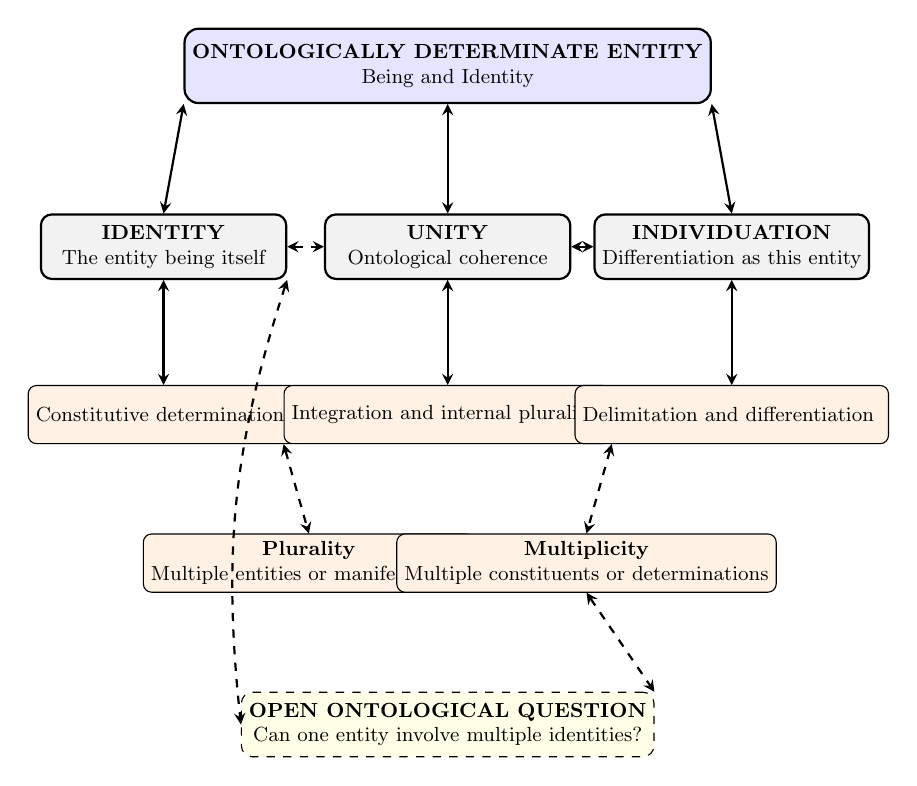
\begin{tikzpicture}[
        scale=0.82,
        transform shape,
        every node/.style={font=\small},
        core/.style={
            rectangle,
            rounded corners=5pt,
            draw=black,
            thick,
            minimum width=4.3cm,
            minimum height=1.15cm,
            align=center,
            fill=blue!10
        },
        concept/.style={
            rectangle,
            rounded corners=4pt,
            draw=black,
            thick,
            minimum width=3.8cm,
            minimum height=1cm,
            align=center,
            fill=gray!10
        },
        dimension/.style={
            rectangle,
            rounded corners=3pt,
            draw=black,
            minimum width=3.5cm,
            minimum height=0.9cm,
            align=center,
            fill=orange!10
        },
        openquestion/.style={
            rectangle,
            rounded corners=4pt,
            draw=black,
            dashed,
            minimum width=4.8cm,
            minimum height=1cm,
            align=center,
            fill=yellow!10
        },
        relation/.style={
            <->,
            thick,
            >=stealth
        },
        analytical/.style={
            <->,
            dashed,
            thick,
            >=stealth
        }
    ]

    % Central ontological entity
    \node[core] (entity) at (0,0) {
        \textbf{ONTOLOGICALLY DETERMINATE ENTITY}\\
        Being and Identity
    };

    % Three analytically distinct dimensions
    \node[concept] (identity) at (-4.4,-2.8) {
        \textbf{IDENTITY}\\
        The entity being itself
    };

    \node[concept] (unity) at (0,-2.8) {
        \textbf{UNITY}\\
        Ontological coherence
    };

    \node[concept] (individuation) at (4.4,-2.8) {
        \textbf{INDIVIDUATION}\\
        Differentiation as this entity
    };

    % Dimensions associated with each concept
    \node[dimension] (constitutive) at (-4.4,-5.4) {
        Constitutive determination
    };

    \node[dimension] (coherence) at (0,-5.4) {
        Integration and internal plurality
    };

    \node[dimension] (distinction) at (4.4,-5.4) {
        Delimitation and differentiation
    };

    % Plurality and multiplicity
    \node[dimension] (plurality) at (-2.15,-7.7) {
        \textbf{Plurality}\\
        Multiple entities or manifestations
    };

    \node[dimension] (multiplicity) at (2.15,-7.7) {
        \textbf{Multiplicity}\\
        Multiple constituents or determinations
    };

    % Open ontological question
    \node[openquestion] (question) at (0,-10.2) {
        \textbf{OPEN ONTOLOGICAL QUESTION}\\
        Can one entity involve multiple identities?
    };

    % Relations between the entity and its dimensions
    \draw[relation] (entity.south west) -- (identity.north);
    \draw[relation] (entity.south) -- (unity.north);
    \draw[relation] (entity.south east) -- (individuation.north);

    % Analytical distinctions
    \draw[analytical] (identity.east) -- (unity.west);
    \draw[analytical] (unity.east) -- (individuation.west);

    % Relations to associated dimensions
    \draw[relation] (identity.south) -- (constitutive.north);
    \draw[relation] (unity.south) -- (coherence.north);
    \draw[relation] (individuation.south) -- (distinction.north);

    % Internal plurality and multiplicity
    \draw[analytical] (coherence.south west) -- (plurality.north);
    \draw[analytical] (coherence.south east) -- (multiplicity.north);

    % The open question is not presented as a settled conclusion
    \draw[analytical] (identity.south east) to[bend right=12]
        (question.west);

    \draw[analytical] (multiplicity.south) -- (question.north east);

    \end{tikzpicture}

    \caption{The Relations Among Identity, Unity, and Individuation: Their Distinct Ontological Dimensions and the Open Question of Multiple Identities Within One Entity}
    \label{fig:identity-unity-and-individuation}
\end{figure}


The figure should be interpreted
as a conceptual representation rather
than as a causal, temporal, or hierarchical
sequence. It does not establish that
identity produces unity, that unity
produces individuation, or that
individuation is temporally subsequent
to identity.

It also preserves the open question
of whether one individual existent
may involve multiple identities.

\subsection{The Limits of an Ontology of Individuation}

The analysis establishes several
constraints for any subsequent
account of individuation.

First, individuation cannot be reduced
to identity, although the two are
ontologically related.

Second, individuation cannot be
identified with unity or with the
aggregation of components.

Third, distinction and qualitative
uniqueness do not provide sufficient
explanations of individuality.

Fourth, no universal principle of
individuation should be assumed
without establishing its applicability
to different kinds of existents.

Fifth, material, structural, and
relational conditions may contribute
to individuation, but their respective
roles must be examined rather than
presumed.

Sixth, individuation does not
automatically resolve the problem
of numerical identity and persistence.

Finally, the possibility of multiple
identities within one individual
existent remains open.

These constraints establish the
conceptual ground for a more precise
analysis of numerical identity and
the conditions under which an
individual remains the same existent.

\subsection{Concluding Formulation}

Individuation is the ontological
problem of how an existent is
constituted as a distinct individual
existent.

It is related to identity because
the individual is the existent whose
determinate character is under
consideration. It is related to unity
because an individual may constitute
a unity, including a unity involving
internal plurality. It is related to
distinction because individuation
concerns the constitution of an
existent as distinct.

Nevertheless, individuation cannot
be reduced to any of these concepts.

The central principle established
in this section is therefore:

\begin{quote}
Individuation concerns the ontological
constitution of an existent as an
individual. It is related to identity,
unity, and distinction, but cannot
be exhaustively explained through
any one of them.
\end{quote}

This principle establishes the basis
for examining numerical identity:
whether an individuated existent
remains one and the same existent
across different conditions and
transformations.



% =============================================================================
% SECTION 07
% IDENTITY AND NUMERICAL IDENTITY
% =============================================================================


\section{Identity and Numerical Identity}
\label{sec:identity-and-numerical-identity}

\subsection{The Ontological Problem of Numerical Identity}

Numerical identity concerns whether an existent considered
under different conditions is one and the same existent.

It must be distinguished from the broader ontological
problem of identity. Identity concerns the determinate
character through which an existent is the existent that
it is. Numerical identity concerns the sameness of an
individual existent across different conditions, states,
or moments of its existence.

The distinction is fundamental.

An account of what constitutes the identity of an existent
does not automatically resolve every question concerning
whether that existent remains numerically the same through
change. Conversely, establishing that an existent is
numerically the same across different conditions does
not provide an exhaustive account of its ontological
identity.

Numerical identity is therefore a specific problem within
the broader ontology of identity. It concerns the sameness
of an individual existent across a relevant comparison,
rather than the total constitution of its identity.

The problem is ontological rather than merely linguistic
or descriptive. The sameness of an existent cannot be
identified with the sameness of the expressions, properties,
or representations through which it may be characterized.

The central question is consequently whether the existent
under consideration remains one and the same existent
across the relevant conditions, and what ontological
conditions are involved in that sameness.

\subsection{Numerical Identity and Qualitative Identity}

A fundamental distinction must be established between
numerical identity and qualitative identity.

Numerical identity concerns whether two references or
considerations concern one and the same existent.

Qualitative identity concerns the sameness of particular
characteristics, properties, or determinations.

Two numerically distinct existents may be qualitatively
indistinguishable with respect to a specified set of
determinations. Conversely, one and the same existent
may undergo qualitative changes while remaining
numerically identical.

These possibilities establish that qualitative sameness
is neither sufficient nor universally necessary for
numerical identity.

If numerical identity were defined through the complete
preservation of qualitative characteristics, every
qualitative change would necessarily imply the termination
of the original existent and the emergence of another.
Such a conclusion cannot be adopted without independently
establishing that the relevant qualities are constitutive
of numerical identity.

Likewise, two existents cannot be considered numerically
identical merely because they share the same qualitative
configuration or because no relevant qualitative
difference has been established.

Qualitative similarity and numerical sameness therefore
belong to different analytical dimensions.

The numerical identity of an existent cannot be reduced
to qualitative resemblance, the coincidence of properties,
or the preservation of a descriptive configuration.

\subsection{Numerical Identity and Individuation}

Numerical identity is closely related to individuation,
but the two concepts address different ontological
questions.

Individuation concerns the ontological constitution
of an existent as an individual. Numerical identity
concerns whether that individual is one and the same
existent across different conditions.

Individuation therefore concerns the constitution
of individuality, whereas numerical identity concerns
the sameness of the individuated existent across
a relevant comparison.

The distinction is important because the constitution
of an existent as an individual under one condition
does not, by itself, resolve whether that individual
continues to exist as the same individual under
subsequent transformations.

An existent may be individuated while questions
concerning its numerical identity remain unresolved.

Conversely, the problem of numerical identity cannot
be adequately formulated without specifying the
individual existent whose sameness is at issue.

The two concepts are consequently mutually relevant
but analytically distinct. Individuation establishes
the problem of the constitution of an individual;
numerical identity establishes the problem of the
sameness of that individual across different conditions.

\subsection{Numerical Identity and Non-Identity}

Numerical identity can be expressed through the
distinction between an existent and any other existent.

If an existent A is numerically identical with an
existent B, A and B are not two distinct existents.
They are one and the same existent considered under
different references or conditions.

If A and B are numerically distinct, they are not
one and the same existent, even if they share
qualitative characteristics or structural configurations.

This distinction must not be confused with differences
between descriptions.

Different descriptions may concern one and the same
existent. Conversely, identical descriptions do not,
by themselves, establish that the existents to which
they are applied are numerically identical.

The ontological question concerns the existent itself,
not merely the expressions or descriptions through
which it is characterized.

Numerical identity therefore cannot be established
exclusively through linguistic equivalence, descriptive
consistency, or the coincidence of predicates.

It concerns the sameness of the existent across
the relevant comparison.

The distinction between numerical identity and
non-identity must also be preserved without assuming
that every difference between determinations constitutes
a difference between individuals.

\subsection{Numerical Identity and Change}

The relation between numerical identity and change
is one of the central problems in the ontology
of identity.

An existent may undergo changes in its properties,
states, relations, material constitution, or structural
organization. The occurrence of such changes does
not automatically establish that the existent has
become numerically different from itself.

However, the possibility of numerical identity
through change does not imply that every possible
transformation is compatible with the continued
existence of the same individual.

The relevant question concerns the ontological
significance of the transformation: which changes
are compatible with the continued numerical identity
of an existent, and which may affect the conditions
under which that existent continues to be the same
individual?

This question cannot be answered by treating all
determinations as equally significant.

Some changes may concern determinations that are
not constitutive of the numerical identity of
the existent. Other changes may affect its
constitutive organization or the conditions
through which it exists as the individual that
it is.

At least three possibilities must therefore
be distinguished:

\begin{itemize}
    \item A change in a determination that does
    not necessarily affect numerical identity.

    \item A change in a potentially constitutive
    determination that raises the question of
    whether numerical identity is preserved.

    \item A transformation that involves the
    termination of one individual and the
    emergence of another.
\end{itemize}

These possibilities must not be collapsed into
a single universal rule.

The ontological significance of a transformation
depends on the constitution of the existent and
the role of the determinations involved.

Numerical identity through change must therefore
be investigated in relation to the specific
conditions of the existent rather than through
an unrestricted assumption that either all
change preserves identity or every significant
change destroys it.

\subsection{Numerical Identity and Persistence}

Persistence concerns the continued existence
of an existent across different conditions.

Numerical identity is central to the problem
of persistence because persistence ordinarily
involves the continuation of one and the same
existent rather than the mere succession of
different existents.

Nevertheless, persistence and numerical identity
must not be treated as interchangeable without
qualification.

Persistence concerns the continuation of existence
across relevant conditions. Numerical identity
concerns whether the existent across those
conditions is one and the same individual.

This distinction makes it possible to examine
the conditions of continued existence without
assuming that every form of continuity establishes
numerical sameness.

An account of persistence must therefore address
the ontological basis of continuity, transformation,
and possible termination.

The present analysis does not assume that
persistence requires the preservation of every
property, determination, or material constituent.
Nor does it assume that the continued existence
of some material components is sufficient to
establish the numerical identity of the whole.

The relation between the persistence of components
and the persistence of the individual configuration
must be examined in its own right.

The conditions under which an individual persists
as numerically the same existent therefore remain
a distinct problem requiring further ontological
analysis.

\subsection{Material Continuity and Numerical Identity}

Material continuity provides one possible dimension
through which the persistence of an existent
may be examined.

An existent may retain some of its material
constituents while undergoing changes in other
aspects of its constitution. Conversely, its
material constitution may undergo substantial
replacement or transformation.

However, material continuity cannot automatically
be equated with numerical identity.

The persistence of particular material components
does not necessarily establish that the same
individual continues to exist. Conversely,
changes in material constitution do not necessarily
imply that the original individual has ceased
to exist.

The significance of material continuity depends
on the ontological nature of the existent and
the role of material constitution in its identity
and persistence.

For some existents, particular material conditions
may be constitutive of their continued numerical
identity. For others, material replacement or
transformation may be compatible with the
persistence of the same individual.

These possibilities cannot be resolved through
a universal assumption about the necessity
or sufficiency of material continuity.

Material continuity is therefore a potentially
significant condition in the analysis of numerical
identity, but it is neither an exhaustive definition
nor an independently sufficient criterion
of numerical sameness.

\subsection{Structural Continuity and Numerical Identity}

Structural continuity provides another dimension
of the problem of numerical identity.

An existent may preserve certain organizational
relations while its components, properties,
or other determinations undergo change.

Such continuity may be relevant to persistence,
particularly where structural organization
contributes significantly to the ontological
constitution of the existent.

Nevertheless, structural continuity cannot
automatically be treated as sufficient for
numerical identity.

Two numerically distinct existents may instantiate
the same structural organization. Conversely,
an individual may undergo structural modifications
without necessarily becoming a numerically
different existent.

The relevant question is whether the structure
under consideration is constitutive of the
individual's identity and whether its alteration
affects the conditions under which that individual
continues to exist.

Structural continuity must therefore be distinguished
from the mere repetition or preservation of
a structural pattern.

A pattern may persist across different existents
without establishing their numerical identity.
Likewise, the modification of a pattern does
not by itself establish the termination of
the individual in which it occurs.

Structural continuity is consequently a potentially
relevant condition of numerical persistence,
but its constitutive significance must be
established in relation to the existent concerned.

\subsection{Relational Continuity and Numerical Identity}

Relational continuity may also contribute
to the examination of numerical identity.

An existent may participate in relations that
persist across different conditions. Some of
these relations may be relevant to its continued
existence as the same individual.

However, the persistence of a relation does
not necessarily establish the persistence
of the individual involved.

A relation may continue to obtain even when
one of the existents participating in it has
been replaced by another. Conversely, the
alteration or termination of a particular
relation does not necessarily imply the
termination of numerical identity.

Relational continuity must therefore be
distinguished from numerical identity itself.

The ontological role of relations must be
examined in relation to the specific existent
and the conditions under which its individuality
and identity are maintained.

In particular, the persistence of a relational
position cannot be treated as an independently
sufficient criterion of numerical sameness.

Likewise, a change in relational conditions
cannot be assumed to produce a new individual
without establishing the constitutive significance
of the relations involved.

Relational continuity is therefore recognized
as a possible condition of numerical persistence,
not as a universal explanation of it.

\subsection{Numerical Identity and Invariance}

Numerical identity is related to the problem
of invariance, but the two concepts must not
be conflated.

Invariance concerns the preservation of a
specified feature, relation, or configuration
under a particular class of transformations.

Numerical identity concerns whether the existent
before and after a transformation is one and
the same existent.

An invariant may provide a basis for investigating
the preservation of identity. However, the
existence of an invariant does not, by itself,
establish numerical identity.

A structural pattern may remain invariant
across different individuals. Conversely,
the numerical identity of an existent may
be preserved even when some of its properties,
relations, or configurations change.

The relation between invariance and numerical
identity therefore depends on the ontological
significance of the invariant under consideration.

A particular invariant may be constitutive
of numerical persistence in a specific kind
of existent. Yet this possibility must be
established independently rather than inferred
from invariance alone.

This distinction is especially important
because invariance has sometimes been used
as a general definition of identity.

The present ontology does not accept the
reduction of identity or numerical identity
to invariance without an independent
ontological justification.

Invariance may be relevant to the analysis
of identity preservation, but it cannot
be presumed to provide a universal criterion
of numerical sameness.

\subsection{Numerical Identity and Signature}

A signature may characterize an existent
through a configuration of identifying features
or determinations.

Such a configuration may be relevant to
the distinction of an existent from others
or to the examination of its different
states and manifestations.

However, a signature is not necessarily
identical to the numerical identity of
the existent.

Two distinct existents may possess
indistinguishable signatures within a
particular descriptive or structural
framework. Likewise, the signature of
one existent may change without necessarily
implying that the existent has been
replaced by another.

The relation between signature and
numerical identity must therefore be
examined without reducing the latter
to the former.

A signature may provide a configuration
through which an existent is characterized,
but its constitutive significance for
numerical persistence must be established
rather than presumed.

The possibility that a signature may
preserve, express, or characterize certain
dimensions of an existent's identity
does not establish that it exhausts
the ontological conditions of numerical
sameness.

The distinction between the existent,
its numerical identity, and its signature
must therefore remain explicit.

\subsection{Numerical Identity and the Problem of Replacement}

The problem of replacement concerns
the conditions under which an existent
ceases to be the same individual and
another existent takes its place.

Replacement must be distinguished
from ordinary change.

An alteration in properties, relations,
or material constituents does not
necessarily constitute replacement.
Conversely, the preservation of certain
features does not necessarily exclude it.

The distinction requires an account
of the conditions that are constitutive
of the continued existence of the
individual.

Several questions therefore arise:

\begin{itemize}
    \item Under what conditions does
    transformation remain compatible
    with the numerical identity of
    an existent?

    \item When does a transformation
    affect the constitution of an
    individual to such an extent that
    its numerical identity is no longer
    preserved?

    \item Can a new existent emerge
    through the material or structural
    transformation of a previous
    existent?

    \item What is the ontological relation
    between the termination of one
    individual and the emergence of
    another?

    \item Can the termination of an
    individual and the emergence of
    another involve continuity in some
    constitutive conditions without
    establishing numerical identity
    between them?
\end{itemize}

These questions cannot be answered
through the mere identification of
qualitative differences or the preservation
of selected characteristics.

The present analysis therefore distinguishes
transformation from replacement while
leaving the specific conditions of
replacement open to further investigation.

In particular, the continuation of
some material, structural, or relational
conditions across a transformation
must not be confused with the numerical
identity of the individual before
and after that transformation.

\subsection{Numerical Identity and the Independence of Ontological Sameness}

Numerical identity belongs to the
ontological constitution and continuity
of the existent. It is not created
or eliminated by changes in the
descriptions or representations
through which an existent is characterized.

An existent may be characterized
under different descriptions without
thereby becoming a different existent.
Likewise, the absence of a description
or the omission of a particular
determination does not establish
the absence of numerical identity.

The distinction is important because
the ontological sameness of an existent
must not be confused with the identity
or difference of its descriptions.

Different descriptive configurations
may concern one and the same existent.
Conversely, the repetition of a
description or configuration does
not establish that two considerations
concern one and the same individual.

The present analysis therefore
treats numerical identity as independent
of descriptive equivalence, representational
continuity, and designation.

The issue is not how sameness is
established through a description,
but what ontological conditions
make an existent numerically the
same existent across different
conditions.

\subsection{The Relation Between Identity and Numerical Identity}

The analysis establishes a necessary
distinction between identity in its
broader ontological sense and
numerical identity as a specific
problem concerning the sameness
of an individual across different
conditions.

Identity concerns the determinate
character of an existent.

Numerical identity concerns whether
the existent considered under
different conditions is one and
the same individual.

The two concepts are related because
numerical identity concerns the
sameness of an existent whose
identity is under consideration.
Nevertheless, numerical identity
does not exhaust the broader
ontological constitution of identity.

Nor can the preservation of numerical
identity be inferred merely from
the persistence of qualitative
characteristics, material constituents,
structural patterns, relations,
invariants, or signatures.

Each of these conditions may be
relevant to the analysis of numerical
sameness, but its ontological role
must be examined independently.

The broader identity of an existent
and the numerical sameness of that
existent must therefore remain
distinct but related dimensions
of the ontology of identity.

\subsection{The Limits of an Ontology of Numerical Identity}

The preceding analysis establishes
several constraints for any subsequent
account of numerical identity.

First, numerical identity cannot
be reduced to the broader ontological
identity of an existent, although
the two are inseparable in the
examination of an individual existent.

Second, numerical identity cannot
be reduced to qualitative sameness
or the coincidence of properties.

Third, individuation and numerical
identity address different questions:
the constitution of an individual
and the sameness of that individual
across different conditions.

Fourth, change does not necessarily
terminate numerical identity, but
not every transformation can be
assumed to preserve it.

Fifth, material, structural, and
relational continuity may contribute
to numerical persistence, but none
can be assumed to constitute a
universal and sufficient criterion.

Sixth, invariance may be relevant
to identity preservation without
being identical to numerical identity.

Seventh, a signature may characterize
an existent without necessarily
exhausting the ontological conditions
of its numerical sameness.

Finally, transformation, replacement,
and the emergence of another existent
must be distinguished through an
examination of their constitutive
conditions rather than through
qualitative difference alone.

These constraints establish the
conceptual basis for examining
signature as a further dimension
of the ontology of identity.

\subsection{Concluding Formulation}

Numerical identity concerns whether
an existent considered under different
conditions is one and the same
existent.

It is a specific dimension of the
broader ontology of identity and
must be distinguished from qualitative
similarity, descriptive sameness,
material continuity, structural
continuity, relational continuity,
invariance, and signature.

These conditions may contribute
to the investigation of numerical
identity, but none can be assumed
to provide a universal and exhaustive
criterion of numerical sameness.

The central principle established
in this section is therefore:

\begin{quote}
Numerical identity concerns the
sameness of an individual existent
across different conditions. It is
a specific dimension of the broader
ontology of identity and cannot
be reduced to the preservation
of qualitative features, material
constituents, structural patterns,
relations, invariants, or descriptive
signatures. Its ontological conditions
must be examined in relation to
the constitution and persistence
of the individual existent concerned.
\end{quote}

This principle establishes the
basis for examining identity and
signature: the relation between
the ontological identity of an
existent and the configuration
through which its determinations
may be characterized.



% =============================================================================
% SECTION 08
% IDENTITY AND SIGNATURE
% =============================================================================

% =============================================================================
% Project : THE_PHILOSOPHY_OF_VIABILITY
% Book    : Book I — Ontology of Viability
% Book ID : VS.B01
%
% File    : 2_MAINMATTER/PART_I_IDENTITY/chapter_01_identity/sections/section_08_identity_and_signature.tex
%
% Section / Chapter:
%   Identity and Signature — Chapter 01: Identity
%
% Purpose :
%   To examine the relation between ontological identity and signature,
%   distinguish signature from determination, invariance, numerical identity,
%   individuation, and manifestation, and clarify the unresolved ontological
%   status of signature.
%
% =============================================================================

\section{Identity and Signature}
\label{sec:identity-and-signature}

\subsection{The Ontological Problem of Signature}

The relation between identity and signature raises a distinct
problem within the ontology of identity: whether an organized
configuration of determinations can characterize an existent
without thereby constituting, or exhausting, its identity.

An existent may involve multiple determinations and relations
that form an organized configuration. Some of these
determinations may be materially, structurally, or relationally
connected. Their configuration may provide a significant basis
for characterizing the existent in a particular respect. The
term \emph{signature} will be used for such an organized
configuration when considered in its characterizing role.

This use of the term does not yet settle the ontological status
of signature. In particular, it does not determine whether a
signature is merely an analytical configuration of actual
determinations, whether it corresponds to a distinct
ontological organization, or whether its status differs across
different kinds of existents.

The central question is therefore not simply whether a
signature can characterize an existent. It is whether the
characterizing role of a signature warrants identifying it
with the existent's identity, or assigning it a constitutive
role in that identity.

The distinction between identity and signature must be
maintained while these possibilities are examined.

Identity concerns what makes an existent the existent that
it is, without presupposing that its identity is reducible
to any single determination or configuration. Signature,
by contrast, concerns an organized configuration of
determinations through which an existent may be characterized
in a particular respect.

The two are related because a signature may involve
determinations that are relevant to the constitution,
character, or differentiation of an existent. Their relation,
however, does not establish their equivalence. Nor does the
fact that a signature characterizes an existent establish
that it provides a complete account of what that existent
is.

The present section therefore rejects the identification
of identity with signature while leaving open the more
specific question of whether, and under what conditions,
signature may participate in the ontological constitution
of identity.

\subsection{Identity Is Not Reducible to Signature}

Identity cannot be defined simply as the signature of an
existent.

Such a definition would make the identity of an existent
equivalent to a configuration of determinations selected
and organized as its signature. This would conflate the
ontological question of what the existent is with the
question of which determinations are brought together
to characterize it.

Several difficulties follow from this reduction.

First, a signature may be selective. It may include some
determinations while omitting others. If identity were
equivalent to signature, every omitted determination
would risk being treated as irrelevant to identity, even
where that determination might be ontologically
constitutive.

Second, signatures may be specified at different levels
of comprehensiveness or under different respects of
consideration. The same existent may consequently admit
different characterizations without there being sufficient
grounds to conclude that its identity has changed.

Third, determinations included in a signature may vary.
A change in one or more of them does not, by itself,
establish a change in numerical identity or in the
ontological constitution of the existent.

Fourth, the same configuration may characterize more
than one numerically distinct existent. A signature's
descriptive or structural distinctiveness within one
domain cannot therefore be assumed to provide a
universal criterion of individuation or numerical identity.

These difficulties do not show that signatures are
ontologically insignificant. They show that their
significance cannot be established by identifying them
with identity in advance.

A signature may be relevant to the constitution or
characterization of an existent. Whether that relevance
is constitutive, conditional, or merely characterizing
must be examined independently.

\subsection{Signature as an Organized Configuration}

A signature is not adequately understood as an arbitrary
list of properties. Its characterizing role depends on
the organization of the determinations involved.

A configuration may be organized through relations among
its determinations, through their arrangement, or through
the way in which they jointly characterize an existent.
The significance of the configuration may therefore
depend not only on which determinations are included,
but also on how they are related.

This does not imply that every signature possesses a
single organizing principle, that its components form
a unified whole, or that the organization is necessarily
intrinsic to the existent. These are further questions
that cannot be settled by the concept of signature alone.

Nor does the organization of a configuration establish
the ontological priority of its components. A determination
may be relevant to a signature without being ontologically
prior to the other determinations involved. Similarly,
the coherence of a configuration does not establish that
all its components are constitutive of identity.

The term signature thus identifies an organized
configuration considered in relation to the
characterization of an existent. It does not, by itself,
determine whether that organization constitutes an
ontological unity, an analytical grouping, or a
combination of both.

This distinction is necessary because an existent's
actual determinations and the configuration through
which some of them are considered are not automatically
the same thing. The determinations may belong to the
existent independently of whether they are grouped
together as a signature.

\subsection{Signature and Determination}

Signature and determination are related but non-equivalent.

Determination concerns the ontological condition through
which an existent is determinate. Signature concerns an
organized configuration involving determinations that
may be relevant to characterizing that existent.

A signature therefore does not constitute the totality
of an existent's determinations merely by bringing
some of them together. Its scope may be selective,
respect-dependent, or limited to a particular
configuration under consideration.

The omission of a determination from a signature does
not establish that the determination is absent from
the existent. Nor does it establish that the omitted
determination lacks ontological significance.

Conversely, the inclusion of a determination in a
signature does not establish that it is constitutive
of identity. Its inclusion establishes, at most, its
relevance to the configuration as specified. The
nature and extent of that relevance require separate
examination.

It is also necessary to distinguish the actual
determinations of an existent from the criteria through
which a signature is specified. A criterion of inclusion
may determine which features are considered together,
but it does not thereby determine which features
actually belong to the existent.

Signature is consequently neither an alternative
name for determination nor an exhaustive inventory
of determination. It is a configuration involving
determinations whose ontological relations and
significance cannot be inferred solely from their
participation in that configuration.

\subsection{The Ontological Status of Signature}

The distinction between identity and signature does
not, by itself, establish what kind of ontological
status signature possesses.

At least three possibilities must be distinguished.

First, a signature may be an analytical configuration:
a grouping of actual determinations considered together
for the purpose of characterizing an existent. On this
account, the configuration as a signature need not
constitute an additional ontological feature of the
existent, even though the determinations grouped
together are real.

Second, a signature may correspond to an organization
that belongs to the existent independently of its
description. In this case, the signature would not
merely collect determinations analytically; it would
also refer to an organization grounded in the existent
itself. Whether such an organization is constitutive
of identity would remain a further question.

Third, signature may have a conditional or domain-specific
ontological significance. Certain configurations may
participate in the constitution of particular kinds
of existents or in particular respects of their
identity, without signature having one universal
ontological function.

These possibilities should not be treated as an
exhaustive classification. They identify distinctions
that must be investigated before a general ontological
account of signature can be established.

In particular, the claim that a signature corresponds
to an actual organization does not entail that it
constitutes identity. Likewise, the claim that a
signature is analytically specified does not entail
that the determinations involved are merely descriptive
or lack ontological significance.

The ontological status of signature therefore remains
an open problem. The present analysis establishes
the non-equivalence of identity and signature, not
a definitive theory of signature's independent
ontological status.

\subsection{Signature and Invariance}

Signature may be related to invariance when some
determinations or relations within a configuration
remain preserved under specified transformations.

Invariance concerns the preservation of a specified
feature, relation, or configuration under a particular
class of transformations and with respect to a
specified domain. Signature concerns an organized
configuration of determinations considered in its
characterizing role.

A signature may contain invariant and variable
determinations. Its configuration may remain stable
under some transformations while changing under
others. Whether such changes affect the relevance
or organization of the signature depends on the
configuration and the transformations being considered.

Conversely, an invariant may be shared by multiple
numerically distinct existents. The preservation of
a feature under transformation therefore does not
necessarily distinguish one existent from another.

Neither the stability of a signature nor the
presence of invariants within it establishes that
the signature is identical to identity. Nor does
the absence of an identified invariant establish
that an existent lacks identity.

An earlier formulation of identity in terms of
invariance under allowable transformations cannot
therefore be transferred into the present account
without additional argument. Such a formulation
would require an independently justified account
of the relevant transformations, the domain of
application, and the respect in which preservation
is being considered.

Invariance may provide a condition for examining
the stability of particular signatures. It cannot
be assumed to provide a universal definition of
signature or identity.

\subsection{Signature and Numerical Identity}

Signature cannot be treated as a sufficient criterion
of numerical identity.

Two numerically distinct existents may possess
identical or indistinguishable signatures within
a specified domain and respect of comparison.
The sameness of their signatures therefore does
not establish that they are one and the same existent.

Conversely, the signature associated with one
existent may change as some of its determinations
or relations change. Such a change does not, by
itself, establish that the existent has ceased
to exist or that another existent has replaced it.

These possibilities show that the comparison of
signatures cannot independently settle the question
of numerical identity. Signature similarity does
not establish numerical identity, and signature
difference does not establish numerical non-identity.

This conclusion must be distinguished from the
question of persistence. Numerical identity concerns
whether different designations or considerations
refer to one and the same existent. Persistence
concerns whether an existent continues to exist
through relevant changes or conditions. A signature
may be relevant to an investigation of persistence,
but its stability is not, without further argument,
a sufficient criterion of persistence.

The ontological role of signature in the continuity
of an existent must therefore be investigated
without presupposing that the preservation of a
signature is either necessary or sufficient for
the persistence of that existent.

\subsection{Signature and Individuation}

Signature may characterize an individual existent
in relation to other existents. It does not thereby
explain how that existent is constituted as an
individual.

Individuation concerns the ontological constitution
of an existent as an individual. Signature concerns
an organized configuration of determinations through
which that individual may be characterized.

A signature may be distinctive within a particular
domain or respect of comparison. Such distinctiveness
may assist in differentiating an existent from
others under those conditions. It does not,
however, establish that the signature provides
the ontological ground of individuation.

Likewise, the absence of a unique signature does
not establish the absence of individuality. Two
numerically distinct individuals may share a
signature, or may be indistinguishable with respect
to the determinations included in a particular
configuration.

It follows that individuality must not be made
dependent upon the possession of an absolutely
unique signature. The possibility of shared
signatures does not eliminate numerical distinction,
just as a distinctive signature does not, by itself,
explain the constitution of an individual.

Signature may therefore contribute to the
characterization of individuality without being
identified with individuation or treated as its
universal ontological ground.

\subsection{Signature and Manifestation}

Signature and manifestation concern different
aspects of an existent.

Manifestation concerns the ways in which an existent
or its determinations become manifest under
particular ontological conditions. Signature
concerns an organized configuration of determinations
through which an existent may be characterized.

A particular manifestation may involve some
determinations associated with a signature without
exhausting that signature. Different manifestations
may also involve different subsets or arrangements
of determinations.

Such variation does not automatically establish
a change in identity. Nor does the fact that a
signature characterizes an existent establish
that the signature is itself a manifestation.

Three questions must therefore remain distinct:

\begin{itemize}
    \item What constitutes the ontological identity
    of an existent?

    \item Which organized configuration of
    determinations characterizes the existent
    in a specified respect?

    \item Under what ontological conditions do
    particular determinations become manifest?
\end{itemize}

These questions may constrain one another, but
their answers cannot be presumed to coincide.

The relation between signature and manifestation
also remains open in a further respect: a signature
may be associated with multiple manifestations,
while a manifestation may involve determinations
that are not included in a particular signature.
The precise relation depends on the organization
and scope of the configuration under consideration.

The present analysis consequently rejects both
the reduction of identity to signature and the
reduction of signature to manifestation.

\subsection{The Possibility of Multiple Signatures}

The distinction between identity and signature
allows for the possibility that one existent may
be characterized through more than one signature.

Different configurations may organize different
determinations or relations, or characterize
different respects of the same existent. Their
differences need not imply that the existent
possesses multiple identities.

Nor should the possibility of multiple signatures
be taken to establish that all such configurations
are equally comprehensive or ontologically
equivalent. One configuration may include
determinations omitted from another; two
configurations may overlap; or they may concern
different domains and respects.

These possibilities require distinctions among
the relations that may hold between signatures.
Overlap does not entail identity of configurations.
Partial inclusion does not establish ontological
priority. Difference between configurations
does not, by itself, establish difference between
the identities of the existents they characterize.

The possibility of multiple signatures must also
be distinguished from the question of whether
one existent can involve multiple identities.
The former concerns the plurality of configurations
through which an existent may be characterized.
The latter concerns the ontological constitution
of identity itself.

The possibility of multiple signatures is therefore
compatible with leaving the multiplicity of identity
unresolved. It neither establishes nor excludes
that possibility.

\subsection{Signature, Description, and Ontological Reality}

The characterization of an existent through a
signature must not be confused with the production
of the existent or its determinations through
description.

An existent does not acquire its identity because
a signature has been specified for it. Its actual
determinations do not depend for their existence
upon whether they have been collected into a
configuration or represented in a description.

A description may select, order, and represent
determinations associated with an existent. The
resulting representation may be more or less
comprehensive, accurate, or adequate to the
configuration it purports to characterize. These
features concern the description and its relation
to what it describes; they do not establish that
the existent itself is constituted by the
description.

The distinction between an actual configuration
and its description is therefore essential.
A description of a signature is not identical
to the signature, if the latter corresponds to
an organization grounded in the existent. If
signature is instead used analytically for a
selected configuration, the description still
does not create the determinations it brings
together.

The absence of a complete description does not
establish the absence of identity, determination,
or an actual organization. Nor does the
specification of a complete description establish
that the identity of the existent has been
exhaustively accounted for.

This preserves the ontological independence
of the existent from its characterization while
leaving open the question of whether signature
refers to an organization that possesses an
ontological status beyond its analytical
specification.

\subsection{The Limits of Signature as an Account of Identity}

The analysis establishes several constraints
on the use of signature within an ontology
of identity.

First, signature is not synonymous with identity.
An organized configuration of determinations
cannot be assumed to exhaust what makes an
existent the existent that it is.

Second, signature is not identical to the totality
of an existent's determinations. A configuration
may be selective without implying that omitted
determinations are absent or ontologically
irrelevant.

Third, the inclusion of a determination in a
signature does not by itself establish that
the determination is constitutive of identity.
Its constitutive significance requires an
independent argument.

Fourth, the organization of a signature does
not establish that it constitutes an ontological
unity or possesses an independent ontological
status.

Fifth, signature must not be reduced to invariance.
A signature may include both variable and
invariant determinations, and an invariant may
be shared by distinct existents.

Sixth, the sameness or difference of signatures
does not independently establish numerical
identity or numerical non-identity.

Seventh, a distinctive signature does not
establish the ontological ground of individuation,
and the absence of a unique signature does
not eliminate individuality.

Eighth, a change in signature does not
automatically establish a change in identity,
the end of an existent, or its replacement.

Ninth, multiple signatures associated with
one existent do not, by themselves, imply
multiple identities.

Finally, neither the analytical specification
of a signature nor its descriptive usefulness
settles its ontological status.

These constraints do not render signature
superfluous. They establish the conditions
under which its significance can be examined
without conflating characterization with
ontological constitution.

Signature remains relevant as a way of
considering organized configurations of
determinations. Whether particular configurations
also participate in the constitution of identity
is a further question, to be settled through
specific ontological arguments rather than
through the concept of signature alone.

\subsection{Conceptual Structure of Identity and Signature}

The distinctions developed in this section
can be summarized by separating identity,
determination, signature, invariance, numerical
identity, individuation, manifestation, and
description according to the questions each
concept addresses.

The following table records these distinctions.
It is an analytical guide, not a final taxonomy
of independent ontological entities or domains.

% =============================================================================
% Project : THE_PHILOSOPHY_OF_VIABILITY
% Book    : Book I — Ontology of Viability
% Book ID : VS.B01
%
% File    : 4_ASSETS/tables/VS.B01.P01.C01.S08.SS15.P001.TL01.identity_signature_conceptual_distinctions.tex
%
% Section / Chapter:
%   Identity and Signature — Chapter 01: Identity
%
% Asset:
%   TL01 — Identity and Signature: Conceptual Distinctions
%
% Purpose :
%   To distinguish identity from signature and related concepts,
%   clarifying their different analytical functions and preventing
%   unsupported ontological reductions.
%
% =============================================================================

\begin{table}[htbp]
    \centering
    \caption{Conceptual Distinctions Between Identity and Signature}
    \label{tab:identity-signature-conceptual-distinctions}

    \small
    \renewcommand{\arraystretch}{1.35}

    \begin{tabular}{p{0.19\textwidth} p{0.35\textwidth} p{0.36\textwidth}}
        \hline
        \textbf{Concept}
        &
        \textbf{Central Concern}
        &
        \textbf{Distinction from Signature}
        \\
        \hline

        Identity
        &
        What makes an existent the existent that it is.
        &
        Cannot be reduced to an organized configuration of determinations.
        \\

        Determination
        &
        The ontological condition through which an existent is determinate.
        &
        Signature involves selected and organized determinations but is not identical to determination as such.
        \\

        Signature
        &
        An organized configuration of determinations through which an existent may be characterized in a particular respect.
        &
        Its ontological status and possible constitutive role require independent examination.
        \\

        Invariance
        &
        The preservation of a specified feature, relation, or configuration under particular transformations.
        &
        May concern the stability of some signature components but does not define signature or identity.
        \\

        Numerical Identity
        &
        Whether different designations or considerations refer to one and the same existent.
        &
        Neither identical nor reducible to the sameness of signatures.
        \\

        Individuation
        &
        The ontological constitution of an existent as an individual.
        &
        A distinctive signature may characterize an individual without establishing its ontological ground.
        \\

        Manifestation
        &
        The ways in which an existent or its determinations become manifest under particular ontological conditions.
        &
        A manifestation may involve some signature determinations without exhausting the signature.
        \\

        Description
        &
        The representation or articulation of an existent or a configuration of its determinations.
        &
        A description of a signature must not be confused with the actual determinations or organization it represents.
        \\

        \hline
    \end{tabular}

    \vspace{0.5em}

    \begin{minipage}{0.92\textwidth}
        \footnotesize
        \textit{Note:} This table distinguishes analytical functions
        and ontological questions. It does not establish that every
        listed concept corresponds to an independent ontological
        entity or that the ontological status of signature has been
        definitively settled.
    \end{minipage}
\end{table}

% =============================================================================
% END OF TABLE TL01
% =============================================================================

The following diagram represents the principal
relations and non-equivalences examined in
this section. It distinguishes the existent
and its determinations from the configuration
considered as a signature and from the
description through which that configuration
may be represented.

% =============================================================================
% Project : THE_PHILOSOPHY_OF_VIABILITY
% Book    : Book I — Ontology of Viability
% Book ID : VS.B01
%
% File    : 4_ASSETS/diagrams/VS.B01.P01.C01.S08.SS15.P001.DG01.identity_signature_conceptual_relations.tex
%
% Section / Chapter:
%   Identity and Signature — Chapter 01: Identity
%
% Asset:
%   DG01 — Identity and Signature: Conceptual Relations
%
% Purpose :
%   To represent the conceptual distinction between an existent,
%   its determinations, an organized configuration considered as
%   a signature, and the description through which that configuration
%   may be represented.
%
% Technical Requirements (preamble):
%   \usepackage{tikz}
%   \usetikzlibrary{arrows.meta, positioning}
%
% =============================================================================

\begin{figure}[htbp]
    \centering
    \hyphenpenalty=10000 \exhyphenpenalty=10000\relax  % no hyphenation inside diagram labels

    \begin{tikzpicture}[
        font=\small,
        node distance=0.9cm and 0.7cm,
        % --- base box ---
        box/.style={
            draw, rounded corners=3pt, align=center,
            text width=3.4cm, minimum height=1.6cm,
            inner sep=5pt, line width=0.7pt
        },
        % --- node roles ---
        onto/.style    ={box, fill=blue!8, draw=blue!55!black},
        analytic/.style={box, dashed, fill=gray!10, draw=black!60},
        % --- arrows ---
        directed/.style={-{Stealth[length=2.5mm]}, thick},
        assoc/.style   ={{Stealth[length=2.2mm]}-{Stealth[length=2.2mm]},
                         thick, dashed}
    ]

    % ---------------------------------------------------------------
    % Grid: three columns, centered on Determinations
    % ---------------------------------------------------------------
    \node[onto] (determinations) {
        \textbf{Determinations}\\[2pt]
        Actual determinations of the existent
    };
    \node[onto, left=of determinations] (identity) {
        \textbf{Identity}\\[2pt]
        What makes the existent the existent that it is
    };
    \node[onto, right=of determinations] (manifestation) {
        \textbf{Manifestation}\\[2pt]
        Manifestation of an existent or its determinations
    };
    \node[onto, above=of determinations] (existent) {
        \textbf{Existent}\\[2pt]
        Ontological actuality
    };

    % ---------------------------------------------------------------
    % Analytical column (below Determinations)
    % ---------------------------------------------------------------
    \node[analytic, below=of determinations] (signature) {
        \textbf{Signature}\\[2pt]
        Organized configuration of determinations
    };
    \node[analytic, below=of signature] (description) {
        \textbf{Description}\\[2pt]
        Representation or articulation of a signature
    };

    % Numerical Identity: same column as Identity, same row as Signature
    \node[onto] (numerical) at (identity |- signature) {
        \textbf{Numerical Identity}\\[2pt]
        Reference to one and the same existent
    };

    % ---------------------------------------------------------------
    % Relations
    % ---------------------------------------------------------------
    \draw[directed] (existent)        -- (determinations);
    \draw[directed] (determinations)  -- (signature);

    \draw[assoc] (existent.west) -| (identity.north);
    \draw[assoc] (determinations)     -- (manifestation);
    \draw[assoc] (signature)          -- (description);
    \draw[assoc] (identity)           -- (numerical);

    % ---------------------------------------------------------------
    % Legend (bottom right, in the empty cell)
    % ---------------------------------------------------------------
    \node[anchor=center, draw=black!30, rounded corners=2pt,
          text width=3.4cm, align=left, font=\scriptsize, inner sep=5pt]
        (legend) at (manifestation |- description) {
        \textbf{Legend}\\[3pt]
        \tikz[baseline=-0.5ex]\draw[rounded corners=1pt, thick, fill=blue!8,
            draw=blue!55!black] (0,-0.1) rectangle (0.5,0.1);\;
        ontological concept\\[2pt]
        \tikz[baseline=-0.5ex]\draw[rounded corners=1pt, thick, dashed,
            fill=gray!10, draw=black!60] (0,-0.1) rectangle (0.5,0.1);\;
        analytical notion\\[2pt]
        \tikz[baseline=-0.5ex]\draw[directed] (0,0) -- (0.5,0);\;
        directed relation\\[2pt]
        \tikz[baseline=-0.5ex]\draw[assoc] (0,0) -- (0.5,0);\;
        association
    };

    % ---------------------------------------------------------------
    % Explanatory note
    % ---------------------------------------------------------------
    \node[below=0.8cm of description, text width=11cm, align=center,
          font=\footnotesize\itshape] (note) {
        Conceptual associations do not establish equivalence,
        causal production, or ontological reduction.
        The constitutive status of signature remains open.
    };

    \end{tikzpicture}

    \caption{Conceptual Relations Between Identity, Determination,
    Signature, and Description}
    \label{fig:identity-signature-conceptual-relations}
\end{figure}

% =============================================================================
% END OF DIAGRAM DG01
% =============================================================================

The diagram is conceptual rather than causal,
temporal, or hierarchical. It does not imply
that identity produces signature, that signature
produces invariance, or that manifestation
follows from signature. Nor does it establish
that signature is an independent ontological
layer.

In particular, the distinction between an
existent's actual determinations, their
organization, and the analytical specification
of a signature must not be mistaken for a
settled account of the ontological status of
that organization. The diagram preserves
the questions that remain open rather than
resolving them through visual arrangement.

\subsection{Concluding Formulation}

Identity and signature are related but
non-equivalent.

Identity concerns what makes an existent
the existent that it is. Signature concerns
an organized configuration of determinations
through which an existent may be characterized
in a particular respect.

A signature may characterize determinations
that are relevant to an existent's constitution.
It may also correspond, in some cases, to an
organization grounded in the existent itself.
Neither possibility establishes that signature
is identical to identity or that it exhausts
the ontological constitution of the existent.

The central principle of this section is
therefore:

\begin{quote}
The signature of an existent is not identical
to its ontological identity. It is an organized
configuration of determinations through which
the existent may be characterized, and whose
ontological status and possible constitutive
role must be established independently.
\end{quote}

This principle preserves the distinction
between an existent, its identity, the
determinations associated with it, and the
configurations through which those
determinations may be considered.

It also leaves open a substantive ontological
question: whether signature is exclusively
a mode of analytical characterization or
whether particular signatures may correspond
to, or participate in, real organizations
within the constitution of existents.

The non-reducibility of identity to signature
does not settle that question. It establishes
the conceptual and ontological distinctions
that any adequate answer must respect.

% =============================================================================
% END OF SECTION 08 OF CHAPTER 01
% =============================================================================



% =============================================================================
% SECTION 09
% IDENTITY AND NON-REDUCTION
% =============================================================================


\section{Identity and Non-Reduction}
\label{sec:identity-and-non-reduction}

\subsection{The Ontological Problem of Reduction}

The preceding sections have examined identity in relation to being, determination, unity, distinction, individuation, numerical identity, and signature. These examinations have established that identity cannot be conceptually identified with any one of these dimensions without an additional ontological argument.

The present section draws together the implications of those distinctions and formulates a general constraint for the ontology of identity: the principle of non-reduction.

Reduction occurs when a particular ontological determination, relation, condition, or mode of manifestation is treated as a sufficient and exhaustive explanation of what an existent is in its identity. Such a reduction may take the form of identifying identity with existence, the aggregation of determinations, unity, difference, individuation, numerical sameness, invariance, signature, structure, composition, material constitution, relational position, or manifestation.

Each of these dimensions may be relevant to identity. Some may participate in its constitution, determination, continuity, or articulation. The problem arises when their relevance is taken to establish their equivalence with identity.

The principle of non-reduction therefore does not deny the ontological significance of these dimensions. It denies that their significance, by itself, establishes their sufficiency as definitions of identity.

\subsection{Being and Identity: Inseparability Without Reduction}

The relation between being and identity provides the fundamental case for understanding non-reduction.

Being and identity are ontologically inseparable, analytically distinguishable, and neither has ontological priority over the other.

An existent does not first exist as an identity-free actuality and subsequently acquire identity as an additional determination. Nor can identity replace being, as though the determinate character of an existent could be considered independently of its actuality.

Consequently, identity cannot be reduced to being, because such a reduction would eliminate the question of the determinate ontological character of what exists. Equally, being cannot be treated as an ontological ground from which identity is subsequently derived.

Their distinction is analytical rather than a division into independently existing components. It permits the examination of different aspects of one ontological actuality without introducing an ontological separation between them.

This relation establishes an important limit for every subsequent account of identity: conceptual distinction must not be confused with ontological independence.

\subsection{Non-Reduction Across Ontological Determinations}

The distinctions developed in this chapter can be brought together through several related principles.

First, identity cannot be exhausted by determination. Although every existent is ontologically determinate, the totality or aggregation of its determinations does not automatically explain its identity. Not every determination is necessarily constitutive, and the accumulation of determinations does not by itself explain the ontological organization through which they belong to a particular existent.

Second, identity cannot be exhausted by unity, structure, or composition. Unity concerns the condition of an existent as a unity, while structure and composition concern aspects of its organization and constitution. These dimensions may be relevant to identity, but neither an account of unity nor an inventory of constituents necessarily establishes the determinate identity of the existent.

Third, identity cannot be reduced to distinction, difference, or individuation. Difference may contribute to the determination of an existent in relation to others, while individuation concerns its constitution as a distinct individual. Neither the establishment of difference nor the explanation of individual constitution necessarily provides a complete account of what that individual is.

Fourth, identity cannot be exhausted by numerical identity. Numerical identity concerns the sameness of an individual existent across different conditions. It does not, by itself, explain the full ontological character of that existent.

Finally, identity cannot be identified with signature or invariance. An organized configuration of determinations may characterize an existent, and the persistence of certain features under specified transformations may reveal aspects of continuity. Nevertheless, neither a signature nor an invariant configuration can be assumed to exhaust identity.

These principles do not establish that determination, unity, structure, composition, difference, individuation, numerical identity, signature, or invariance are ontologically independent of identity. They establish only that their respective explanatory roles cannot be presumed to be equivalent to identity itself.

\subsection{Material, Relational, and Manifestational Conditions}

The same principle applies to material constitution, relational determination, and manifestation.

Material constitution may participate in the identity of an existent. In some cases, particular material conditions may be essential to what an existent is; in others, material transformation may occur without necessarily establishing the loss of identity. Neither universal material continuity nor universal material replaceability can be assumed.

Relational determinations may likewise contribute to identity. An existent may be constituted or determined partly through relations with other existents, structural arrangements, or particular conditions. However, relational dependence does not establish that identity is reducible to relational position alone.

Manifestation introduces a further dimension. The way an existent becomes actual or expressed within a particular ontological context may disclose or realize aspects of its determinate character. Yet a particular manifestation cannot automatically be treated as an exhaustive account of identity. Differences between manifestations do not, by themselves, establish differences in the identity of the existent.

These cases demonstrate that the rejection of reduction must not be confused with the rejection of constitutive participation. Material, relational, structural, and manifestational dimensions may be involved in identity without being conceptually interchangeable with it.

Their precise ontological roles remain matters for further investigation.

\subsection{Conceptual Distinction, Ontological Distinction, and Relational Determination}

The principle of non-reduction requires a careful distinction among three levels of analysis.

\begin{enumerate}
    \item \textbf{Conceptual distinction:} Two concepts may express different meanings or explanatory functions without thereby referring to independently existing entities.

    \item \textbf{Ontological distinction:} Two aspects, determinations, or entities may be distinct in being. Such a claim requires an ontological argument and cannot be inferred from conceptual difference alone.

    \item \textbf{Relational determination:} Distinct concepts or ontological aspects may be related through conditions of dependence, constitution, participation, or interaction.
\end{enumerate}

These levels must not be conflated.

The fact that identity and unity are conceptually distinguishable does not, by itself, establish that they are independently existing ontological entities. Likewise, the fact that two dimensions are ontologically distinct does not establish that they are unrelated. A relation of constitution or dependence may connect dimensions that remain distinguishable.

Non-reduction therefore operates first as a constraint against conceptual equivalence. Whether the concepts involved also correspond to distinct ontological determinations, and how they are related, must be established separately.

This distinction prevents two opposite errors: reducing identity to another concept merely because the two are related, and isolating identity from other determinations merely because the concepts are distinguishable.

\subsection{Non-Reduction and Ontological Explanation}

The principle of non-reduction does not provide a complete explanation of identity. Rather, it establishes conditions that an adequate explanation must respect.

An ontological account of identity must examine the roles played by the different dimensions of an existent without assuming in advance that any one of them is sufficient. It must also distinguish among different forms of ontological relevance.

A determination may be constitutive of identity in one case but contingent in another. A relation may be necessary under particular conditions without being universally necessary. A structural or material feature may contribute to the identity of a particular kind of existent without providing a general definition applicable to every existent.

Accordingly, the following questions must remain distinguishable:

\begin{itemize}
    \item Whether a dimension is related to identity.
    \item Whether it participates in the constitution or determination of identity.
    \item Whether it is necessary or sufficient under specified ontological conditions.
    \item Whether its relevance is universal or limited to particular kinds of existents.
    \item Whether its alteration affects identity, continuity, or numerical identity.
\end{itemize}

No answer to one of these questions automatically determines the answers to the others.

Non-reduction thus requires more than the preservation of conceptual distinctions. It requires that claims about constitution, dependence, necessity, sufficiency, and continuity be justified independently rather than inferred from conceptual association.

\subsection{The Question of Multiple Identities}

The non-reduction of identity also leaves open the possibility that one existent may involve more than one identity.

The distinctions developed in this chapter do not provide sufficient grounds for either affirming or rejecting this possibility. The unity of an existent does not necessarily establish that it possesses only one identity. Conversely, internal plurality, compositional complexity, or structural differentiation does not establish that it possesses several identities.

Nor can multiple signatures, material configurations, structural arrangements, or manifestations be treated as evidence of multiple identities without further argument.

The question requires a more precise account of the relation between identity, unity, individuation, and the ontological constitution of an existent. In particular, it remains necessary to determine whether distinct identity determinations could belong to one and the same existent without implying the existence of multiple individuals.

This possibility must therefore remain an open ontological problem. It cannot be resolved merely by extending the conceptual distinctions established in the present chapter.

\subsection{The Principle of Non-Reduction}

The argument of this section can be summarized in the following principle:

\begin{quote}
Identity is not conceptually equivalent to any single ontological determination, condition, relation, or mode of manifestation associated with an existent. Its relation to being, determination, unity, distinction, individuation, numerical identity, signature, invariance, structure, composition, material constitution, relational determination, and manifestation must be examined without presuming that any one of these dimensions exhausts its ontological character. Their possible constitutive, relational, or explanatory relevance remains open to investigation.
\end{quote}

This principle establishes neither the absolute independence of identity nor the ontological independence of every concept related to it. It preserves the distinction between conceptual non-equivalence and ontological separation.

Being and identity remain ontologically inseparable, while the other dimensions examined in this chapter may participate in the constitution, determination, continuity, or manifestation of an existent in ways that require further justification.

Non-reduction is therefore a constraint on ontological explanation rather than a substitute for one. It prevents a partial determination from being treated as a complete account while preserving the possibility of discovering the relations through which the identity of an existent is constituted.

The problem of identity must consequently be pursued through an account that maintains conceptual distinction and ontological relation together.

\subsection{Transition to the Scope and Limits of Identity}

Having established that identity cannot be exhausted by any single related ontological concept, the investigation must now clarify the scope of the claims made about identity.

Non-reduction establishes what cannot be presumed about the relation between identity and its associated dimensions. It does not, by itself, determine the full extent of identity, the conditions under which particular determinations are constitutive, or the limits of the present account.

The following section therefore examines the scope and limits of identity as an ontological concept. Its purpose is to clarify what the present investigation has established, what remains provisional, and which questions must be reserved for subsequent parts of the ontology of viability.



% =============================================================================
% SECTION 10
% SCOPE AND LIMITS OF IDENTITY
% =============================================================================

% =============================================================================
% Project : THE_PHILOSOPHY_OF_VIABILITY
% Book    : Book I — Ontology of Viability
% Book ID : VS.B01
%
% File    : 2_MAINMATTER/PART_I_IDENTITY/chapter_01_identity/sections/section_10_scope_and_limits_of_identity.tex
%
% Section / Chapter:
%   The Scope and Limits of Identity
%
% Purpose :
%   To delimit the ontological claims established in the chapter,
%   distinguish foundational commitments from argued conclusions
%   and provisional constructions, and identify the principal
%   unresolved problems concerning identity.
%
% =============================================================================

\section{The Scope and Limits of Identity}
\label{sec:scope-and-limits-of-identity}

\subsection{The Need to Define the Scope of Ontological Claims}

An ontological investigation must establish not only the
distinctions through which a problem can be examined, but also
the limits of the claims that those distinctions support.

Without an explicit account of scope, conclusions may be
extended beyond the conditions under which they have been
established. A conceptual distinction may be mistaken for an
ontological separation, a possible relation may be treated
as a necessary one, or a partial explanation may be presented
as a universal principle.

The preceding sections have developed a framework for
investigating identity through its relations to being,
determination, unity, distinction, individuation, numerical
identity, and signature. They have also established a
constraint against reducing identity to any one of these
dimensions.

These conclusions clarify the conceptual and ontological
questions that an investigation of identity must address.
They do not, however, constitute a complete account of every
condition under which identity is constituted, maintained,
transformed, or manifested.

The purpose of this section is therefore to delimit the
scope of the present account, clarify the status of its
principal claims, and distinguish what has been established
from what remains provisional or unresolved.

The limits identified here concern the extent of the
arguments developed in this chapter. They must not be
confused with limits imposed upon existence or with claims
about what can or cannot be established by subsequent
ontological inquiry.

\subsection{The Ontological Scope of Identity}

The subject of this chapter is the ontological character
of identity.

Its central question concerns what makes an existent the
existent that it is. This question concerns the existent
itself and does not depend upon an act through which it is
identified, classified, named, or described.

Identity is therefore not treated as a product of
identification or as a determination introduced merely
through an external act. Its ontological status belongs
to the existent rather than to an activity directed toward it.

Within this scope, the chapter has examined the following
relations and distinctions:

\begin{enumerate}
    \item The ontological relation between being and identity.
    \item The relation between identity and determination.
    \item The distinction between identity and unity.
    \item The relations among identity, distinction, and difference.
    \item The relation between identity and individuation.
    \item The distinction between identity and numerical identity.
    \item The relation between identity and signature.
    \item The non-reduction of identity to other related
    ontological dimensions.
\end{enumerate}

These examinations establish a conceptual framework for
the further investigation of identity. They do not establish
that every existent has the same constitutive conditions,
that every dimension examined is relevant in every case,
or that the relations identified operate uniformly across
all possible kinds of existents.

The scope of the chapter is thus general in its ontological
question, but limited in the extent of the constitutive
principles it has established.

\subsection{Identity and Identification}

An important boundary of the present investigation concerns
the distinction between identity and identification.

An existent does not acquire its identity because an act
of identification occurs. Nor does the absence of such an
act imply the absence of identity.

The ontological character of an existent is not constituted
by its being named, classified, distinguished, or recognized
by another existent. Such activities may concern an
existent, but they do not provide the ontological ground
of its identity.

This commitment does not require a theory of identification,
nor does it determine the conditions under which identity
may become accessible to another existent. Those questions
concern additional relations and processes that are not
the subject of the present chapter.

The distinction is more limited and more fundamental:
the identity of an existent must not be made ontologically
dependent upon the occurrence of an identifying activity.

Accordingly, the present account treats identity as an
ontological question independently of whether identification
takes place. This does not entail that every possible
relation between an existent and another existent is
irrelevant to identity. It excludes only the assumption
that an act of identification is itself the ground from
which identity derives.

\subsection{The Limits of a Universal Definition}

The analysis developed in this chapter does not establish
a single universal principle that exhaustively determines
identity in every possible existent.

A principle may explain a particular dimension of identity
without explaining its complete ontological character.
An account of individuation, for example, may address the
constitution of an existent as an individual. An account
of invariance may address the preservation of selected
features or relations under specified transformations.
Neither explanatory function, by itself, establishes
a universal definition of identity.

The same limitation applies to principles based exclusively
on material continuity, structural organization, relational
stability, numerical identity, or the preservation of
a signature.

The present investigation therefore does not claim that
any one of these principles provides a universally
necessary and sufficient criterion of identity.

This limitation must be interpreted carefully. The absence
of an established universal criterion does not imply that
identity has no ontological conditions, nor does it imply
that such conditions are arbitrary. It means that their
general form, necessity, sufficiency, and domain of
applicability have not been established by the arguments
developed in this chapter.

Whether a more comprehensive principle can be formulated
remains an open problem.

The possibility of a universal account must therefore
be distinguished from the claim that such an account has
already been established. The former remains available
for investigation; the latter would exceed the present
argument.

\subsection{The Limits of Claims Concerning Persistence and Transformation}

Identity raises the question of how an existent remains
the existent that it is under different conditions and
through transformation.

The distinctions developed in this chapter prevent change
from being treated as automatically equivalent to the
loss of identity. They do not, however, establish a
universal criterion by which every transformation can
be classified as compatible or incompatible with the
persistence of an existent.

Material, structural, relational, and other determinations
may change in different ways and with different consequences.
Their significance cannot be assumed to be identical
across all kinds of existents.

Accordingly, the following distinctions must be maintained:

\begin{enumerate}
    \item Change does not necessarily entail the loss
    of identity.

    \item The continuity of selected determinations
    does not necessarily establish the persistence
    of identity.

    \item The preservation of a structure, signature,
    or invariant does not, by itself, establish
    numerical identity.

    \item The alteration or replacement of constituents
    does not, by itself, establish the destruction
    of an existent.

    \item Numerical identity across different conditions
    does not provide a complete explanation of the
    ontological character of the existent.

    \item The persistence of an existent and the
    preservation of every determination associated
    with it are not equivalent claims.
\end{enumerate}

These distinctions do not determine which transformations
preserve identity or which conditions are necessary for
persistence. They prevent such determinations from being
inferred solely from the presence or absence of selected
features.

A more comprehensive account must examine the relations
among identity, transformation, continuity, discontinuity,
replacement, and numerical identity in relation to the
kinds of existents and conditions under consideration.

The present chapter establishes the need for this
investigation, not its final criteria.

\subsection{The Limits of Claims Concerning Multiple Identities}

The present chapter does not establish whether one
existent can involve more than one identity.

The unity of an existent does not necessarily demonstrate
that its identity is singular in every relevant
ontological sense. Conversely, internal plurality,
compositional complexity, or structural differentiation
does not establish the existence of multiple identities.

The existence of multiple signatures, configurations,
determinations, or manifestations likewise does not entail
the existence of multiple identities. Such multiplicity
may concern different aspects or conditions of one
existent rather than distinct identity determinations.

The question requires a more precise account of the
relations among identity, unity, individuation, and the
ontological constitution of an existent. In particular,
it remains necessary to determine whether distinct
identity determinations could belong to one and the same
existent without implying the existence of multiple
individuals.

This inquiry must distinguish the possible multiplicity
of identity determinations from the numerical multiplicity
of individuals. The former, if established, would not
automatically entail the latter.

Neither the universal singularity nor the possible
plurality of identity can therefore be asserted on the
basis of the distinctions established so far.

The question remains open for subsequent ontological
investigation.

\subsection{The Limits of Universality Across Domains of Existence}

The conceptual framework developed in this chapter is
intended to support a general ontological investigation.
Nevertheless, its applicability across different domains
of existence does not establish that all identity-related
conditions operate identically in every domain.

A general ontological concept may retain its conceptual
function while the determinations through which it is
constituted or manifested vary according to the nature
of the existent.

Material constitution, structural organization, and
relational determination, for example, may have different
forms or degrees of relevance in different domains.
Such variation does not necessarily imply that identity
itself has an entirely different meaning in each domain.

Conversely, conceptual uniformity does not establish
that the ontological conditions of identity are uniform
throughout existence.

The present chapter therefore establishes neither the
complete uniformity nor the fundamental heterogeneity
of identity across all domains. It provides a general
conceptual framework whose applicability to particular
domains requires further examination.

The investigation of different realms of being must
determine how identity relates to their particular
ontological conditions without presupposing either
universal uniformity or absolute discontinuity.

The term ``domain'' is used here to designate a scope
within which particular ontological conditions are
examined. Its use does not establish a definitive
classification or hierarchy of domains, nor does it
presuppose that the proposed organization of the ontology
of viability is exhaustive.

\subsection{The Limits of the Relationship Between Identity and Manifestation}

The relation between identity and manifestation remains
only partially determined within the present investigation.

The chapter has established that identity cannot be
reduced to manifestation and that a particular
manifestation cannot automatically be treated as an
exhaustive account of the identity of an existent.

This does not establish that manifestation is merely
external to identity, or that the identity of an existent
remains unaffected by every possible condition of
manifestation.

A manifestation may involve particular determinations
of an existent under conditions associated with a
specific ontological context or domain. Whether such
conditions participate in the constitution, realization,
or transformation of identity requires further analysis.

The present chapter does not determine the complete
ontological status of manifestation or expression, nor
does it establish the relations among the domains in
which manifestation occurs.

These matters must be examined in the broader
investigation of manifestation and the realms of being.
Their relationship to identity cannot be settled merely
by the conceptual distinctions established here.

\subsection{The Limits of the Present Conceptual Framework}

The distinctions developed in this chapter provide
necessary conceptual conditions for a more comprehensive
ontology of identity. They do not yet provide a complete
account of its constitutive principles.

Several questions remain unresolved:

\begin{enumerate}
    \item What are the necessary and sufficient ontological
    conditions of identity?

    \item Can a general principle of identity be established
    across different domains of existence?

    \item How can constitutive determinations be distinguished
    from non-constitutive determinations in a general
    ontological account?

    \item Under what conditions can identity persist
    through substantial transformation?

    \item What is the complete relationship between
    identity, individuation, and numerical identity?

    \item Can one existent involve multiple identities
    without implying multiple individuals?

    \item What is the precise ontological relationship
    between identity and manifestation?

    \item To what extent are structure, composition,
    material constitution, and relational determination
    constitutive of identity?
\end{enumerate}

These questions identify the limits of the present account.
Their unresolved status does not, by itself, constitute
a contradiction within the framework or provide evidence
against its foundational commitments.

An unresolved question must not be treated as an
established conclusion. Equally, the absence of a
demonstrated principle must not be interpreted as proof
that such a principle is impossible.

The distinction between what has been established and
what remains open is therefore essential to the continued
development of the ontology.

\subsection{The Status of the Claims Developed in This Chapter}

The claims developed in this chapter must be distinguished
according to their argumentative and justificatory status.
Not all claims have the same function, and not all possess
the same degree or kind of support.

The following commitments provide the foundational
orientation of the present investigation:

\begin{enumerate}
    \item Being and identity are ontologically inseparable
    and analytically distinguishable.

    \item Neither being nor identity has ontological
    priority over the other.

    \item Identity is not an additional property attached
    to an identity-free existent.

    \item The ontological status of identity does not
    depend upon an act of identification.
\end{enumerate}

These commitments define the starting orientation of
the chapter. Their foundational role must not be confused
with the claim that every implication of them has already
been demonstrated.

The following distinctions have been developed through
the conceptual and argumentative analysis of the chapter:

\begin{enumerate}
    \item Identity is not conceptually equivalent to
    determination, unity, distinction, individuation,
    numerical identity, or signature.

    \item Conceptual non-equivalence does not establish
    ontological separation.

    \item Non-reduction does not imply ontological isolation.

    \item No single related ontological dimension has
    been established as an exhaustive definition
    of identity.
\end{enumerate}

These are conclusions of the chapter's analysis. Their
scope is limited to the arguments supporting them and
does not extend automatically to every possible
ontological relation among the dimensions concerned.

The following matters remain provisional or require
further ontological justification:

\begin{enumerate}
    \item The precise constitutive roles of material,
    structural, and relational determinations.

    \item The conditions under which particular
    transformations preserve or alter identity.

    \item The applicability of general identity principles
    across different domains of existence.

    \item The precise relation between identity and
    manifestation.
\end{enumerate}

The following remain open ontological problems:

\begin{enumerate}
    \item Whether a universal principle of identity
    can be established.

    \item Whether one existent can involve multiple
    identities.

    \item What constitutes a complete account of the
    necessary and sufficient conditions of identity.

    \item How identity, individuation, continuity,
    and numerical identity are related in a
    comprehensive ontology.
\end{enumerate}

This classification is local to the present chapter.
It is not a replacement for the broader system of
epistemic and justificatory statuses adopted by the
project. In particular, foundational commitments,
stipulated or defined claims, argued or derived claims,
conditionally supported claims, provisional constructions,
hypotheses, and unresolved problems remain distinguishable
within that broader system.

The classification above identifies the principal
groups of claims relevant to the present chapter; it
does not assign every individual proposition a final
status within the complete ontology.

Nor is this classification intended to establish a
permanent boundary around the theory. It clarifies
the current status of its claims and allows subsequent
arguments to develop, qualify, or revise them without
confusing foundational commitments with unresolved
possibilities.

\subsection{Ontological Restraint and the Development of the Theory}

The limits established in this section concern the
extent of the ontological claims justified by the
present investigation. They are not limitations
imposed upon existence itself.

Ontological restraint requires that the scope of every
claim remain proportionate to the argument supporting it.

A conceptual distinction may be established without
resolving every ontological relation between the
concepts involved. A possible condition may be
identified without being affirmed as universally
necessary or actual. A provisional construction may
organize further inquiry without being treated as a
completed ontological foundation.

This restraint is not a suspension of ontological
inquiry. It is a condition for its systematic development.

It also requires that the absence of a demonstrated
explanation be distinguished from the absence of an
ontological relation. The fact that a constitutive
relation has not yet been established does not show
that no such relation exists. Likewise, identifying
a possible relation does not establish that it is
necessary, universal, or sufficient.

The ontology of viability must therefore preserve
the distinctions among foundational commitments,
stipulated or defined claims, argued or derived claims,
conditionally supported claims, provisional constructions,
hypotheses, and open problems throughout its subsequent
development.

Such distinctions allow the theory to develop without
prematurely universalizing partial results or treating
unresolved questions as though they had already been
answered.

\subsection{Concluding Formulation}

The scope of the present investigation is the
ontological character of identity as inseparable from
the being of an existent. Its limits concern the extent
to which the constitutive conditions, principles, and
relations of identity have been established by the
arguments developed in this chapter.

The argument of this chapter supports the following
formulation:

\begin{quote}
Identity is an ontological dimension inseparable from
the being of an existent, but its complete constitution
cannot be inferred from any single related determination,
condition, or relation. The distinctions developed in
this chapter provide the conceptual conditions for
investigating identity without prematurely asserting
a universal criterion, a complete theory of persistence,
the singularity or plurality of identities, or an
exhaustive account of the relationship between identity
and manifestation.
\end{quote}

The present account establishes a foundational framework
for the ontology of identity, not a complete theory of
every condition under which identity is constituted,
maintained, transformed, or manifested.

Its unresolved questions define the direction of further
ontological inquiry rather than a deficiency in the
reality being investigated.

The chapter can therefore conclude with a distinction
between the ontological problem itself and the limits
of its present formulation: the identity of an existent
is not exhausted by the concepts through which it has
been examined, while the relations among those concepts
remain necessary subjects of further investigation.

The subsequent synthesis must preserve both sides of
this commitment: the ontological inseparability of being
and identity, and the need to investigate identity
without reducing it to any single related determination.

% =============================================================================
% END OF SECTION 10 OF CHAPTER 01
% =============================================================================


% =============================================================================
% SECTION 11
% SYNTHESIS OF IDENTITY
% =============================================================================

% =============================================================================
% Project : THE_PHILOSOPHY_OF_VIABILITY
% Book    : Book I — Ontology of Viability
% Book ID : VS.B01
%
% File    : 2_MAINMATTER/PART_I_IDENTITY/chapter_01_identity/sections/section_11_synthesis_of_identity.tex
%
% Section / Chapter:
%   Synthesis of Identity
%
% Purpose :
%   To synthesize the ontological commitments and arguments
%   developed throughout Chapter 01, preserve the distinctions
%   established among identity and its related dimensions, and
%   identify the unresolved problems that guide subsequent inquiry.
%
% =============================================================================

\section{Synthesis of Identity}
\label{sec:synthesis-of-identity}

\subsection{The Need for an Ontological Synthesis}

The preceding sections have examined identity through a
series of distinctions necessary for establishing its
ontological status. Being, determination, unity, distinction,
individuation, numerical identity, and signature have each
been considered in relation to identity. The investigation
has also examined the limits of reducing identity to
invariance, structure, composition, material constitution,
relational determination, or manifestation.

These distinctions are not intended to fragment the
ontological problem into unrelated conceptual domains.
Their purpose is to prevent the premature identification
of identity with any single dimension of existence while
making it possible to investigate the relations through
which identity may be constituted and determined.

A synthesis is therefore required. It must preserve the
distinctions established throughout the chapter while
bringing their implications together within a coherent
ontological position.

The objective is not to introduce a new principle that
replaces the preceding analysis, nor to claim that every
constitutive condition of identity has already been
discovered. It is to identify the commitments that can
be maintained at the present stage of the investigation,
the conclusions supported by the chapter's arguments,
and the problems that remain unresolved.

The synthesis must consequently preserve two requirements:
identity must not be reduced to any single related
ontological dimension, and its relations to those
dimensions must not be dismissed merely because they
are conceptually distinguishable.

\subsection{Identity as an Ontological Dimension of Existence}

The central foundational commitment of this chapter is
that identity is ontologically inseparable from being.

An existent does not first exist as an identity-free
substrate and subsequently acquire an identity. Being
and identity are not successive conditions, nor are they
two independently existing components that must be
externally combined.

Their distinction is analytical rather than ontologically
separative.

Being concerns the actuality of an existent, while
identity concerns what makes that existent the existent
that it is. These formulations address distinguishable
ontological questions without dividing the existent
into independently actual components.

Neither dimension can be removed from the relation
without altering the meaning of the other. This
inseparability, however, does not establish their
conceptual equivalence or make either one an exhaustive
definition of the other.

Identity must consequently be understood neither as
an additional property attached to an already constituted
identity-free existent nor as a merely descriptive
designation imposed upon it.

This position establishes the ontological significance
of identity without claiming that its complete
constitution has already been explained.

\subsection{Identity and Determination}

The relation between identity and determination is
essential to understanding the determinate character
of an existent.

An existent cannot be adequately considered as though
it were wholly indeterminate. Its being involves
determinations through which it is constituted and
through which its particular ontological character
may be investigated.

Nevertheless, identity cannot be identified with
determination as such, nor can it be reduced to the
accumulation or enumeration of an existent's
determinations.

Not every determination necessarily contributes to
identity in the same manner. Some determinations may
participate in constitution, while others may be
contingent, relational, situational, or dependent upon
particular conditions.

The distinction between determination in general
and determinations that may be constitutive of identity
is therefore essential.

Identity is related to determination because the
ontological character of an existent cannot be
investigated without considering its determinate
conditions. Yet this relation does not establish
that identity is identical with the totality of those
conditions or that their enumeration provides an
exhaustive explanation of identity.

The precise roles of particular determinations,
including their necessity, sufficiency, and possible
constitutive relations, remain subjects for further
ontological investigation.

\subsection{Identity and Unity}

Identity and unity are related but non-equivalent.

Unity concerns the constitution of an existent as a
unity, whereas identity concerns what makes that
existent the existent that it is.

The unity of an existent does not necessarily eliminate
internal plurality, compositional complexity, or
structural differentiation. Conversely, the identity
of an existent does not, by itself, explain every
condition through which its unity is constituted.

Unity therefore cannot serve as an exhaustive
definition of identity.

Nor does the distinction between identity and unity
establish that they are ontologically independent.
Their relation may involve conditions of constitution,
dependence, or participation that require further
argument.

The question of whether one existent may involve
multiple identity determinations also remains distinct
from the question of how that existent constitutes
a unity. Neither question can be resolved merely
by assuming that unity entails singularity of identity
or that internal plurality entails multiplicity of
identities.

\subsection{Identity, Distinction, and Difference}

Identity, distinction, and difference address related
but distinguishable ontological questions.

Identity concerns what makes an existent the existent
that it is. Distinction concerns the grounds upon which
entities, aspects, or determinations are distinguishable.
Difference concerns the ways in which determinations
or existents are non-identical or dissimilar.

An existent is not adequately characterized merely
by establishing that it differs from another existent.
Its identity cannot be reduced to its position within
a system of differences.

Likewise, the distinction of an existent from another
does not, by itself, explain the ontological character
of the existent being distinguished.

Nevertheless, difference and distinction may participate
in the determination of an existent. Their significance
depends upon the particular ontological relations and
conditions involved.

The synthesis therefore preserves both the
non-equivalence of identity and difference and the
possibility that distinction and difference contribute
to the determination of identity.

\subsection{Identity, Individuation, and Numerical Identity}

The relationship between identity and individuation
concerns the constitution of an existent as an individual.

Individuation addresses how an existent is constituted
as an individual, but an account of individual
constitution does not necessarily explain the complete
ontological character of that individual.

Numerical identity introduces a further distinction.
It concerns whether what is considered under different
references, descriptions, or conditions is one and
the same existent.

This question is essential to the examination of
sameness across different conditions, but it does
not provide an exhaustive definition of identity
or a complete account of persistence.

The three concepts therefore address related but
distinguishable ontological problems:

\begin{enumerate}
    \item \textbf{Identity} concerns what makes an
    existent the existent that it is.

    \item \textbf{Individuation} concerns the
    ontological constitution of an existent as
    an individual.

    \item \textbf{Numerical identity} concerns whether
    what is considered under different references
    or conditions is one and the same existent.
\end{enumerate}

Their relationships must be examined together without
treating them as interchangeable.

In particular, the question of how an existent is
individuated must remain distinguishable from the
question of whether it persists as numerically the
same existent through transformation.

\subsection{Identity and Signature}

A signature may provide an organized configuration
of determinations, relations, or features through
which aspects of an existent can be characterized.

Such a configuration may be relevant to the examination
of identity, but it cannot automatically be identified
with identity itself.

The existence of a signature does not establish that
every ontological determination of an existent has
been captured by it. Nor does the possibility of
multiple signatures necessarily imply the existence
of multiple identities.

Likewise, the alteration of a signature does not,
by itself, establish the loss of numerical identity.
The relation between a signature and the constitution
of identity must be examined rather than assumed.

The distinction between identity and signature is
therefore essential to preventing a descriptive or
configurational account from being treated as an
exhaustive ontological account.

The precise ontological status of signature and its
possible role in the constitution, determination,
or characterization of identity remain subjects
for further investigation.

\subsection{The Non-Reduction of Identity}

The preceding distinctions converge upon a general
ontological constraint: identity cannot be reduced
to any single related concept or determination
examined in this chapter.

It cannot be exhausted by being, determination,
unity, distinction, difference, individuation,
numerical identity, or signature. Nor can it be
exhaustively defined through invariance, structure,
composition, material constitution, relational
position, or manifestation.

However, non-reduction does not imply that identity
is isolated from these dimensions.

Each may participate in the constitution,
determination, continuity, differentiation, or
manifestation of an existent. Their precise roles
must be established through appropriate ontological
arguments rather than assumed in advance.

The synthesis therefore requires two simultaneous
commitments:

\begin{enumerate}
    \item Identity must remain conceptually
    distinguishable from its related ontological
    dimensions.

    \item The possible ontological relations among
    identity and those dimensions must remain open
    to investigation.
\end{enumerate}

These commitments prevent both reductionism and
ontological isolation.

The first prevents the explanatory role of a
particular dimension from being treated as proof
of its equivalence with identity. The second
prevents conceptual distinction from being
mistaken for the absence of ontological relations.

Non-reduction thus provides a constraint for
investigating identity without prejudging the
specific relations through which its constitution
may be understood.

\subsection{Identity and the Problem of Persistence}

The ontological status of identity raises the
question of how an existent remains the existent
that it is under changing conditions.

The present chapter establishes that change does
not automatically entail the loss of identity.
It also establishes that the continuity of selected
features does not automatically demonstrate the
preservation of identity.

Neither material continuity, structural persistence,
relational stability, nor the invariance of selected
determinations has been established as a universally
sufficient criterion.

The relationship between identity and persistence
must therefore be investigated through the specific
ontological conditions of the existent under
consideration.

A comprehensive account must eventually explain
how identity relates to transformation without
assuming either that all change destroys identity
or that every transformation is compatible with
its persistence.

It must also distinguish the persistence of an
existent from the preservation of every determination
associated with it, and distinguish both from
the question of numerical identity.

These problems remain open for further development.
Their resolution belongs to a more comprehensive
investigation of continuity, transformation, and
the conditions under which an existent persists.

\subsection{Identity and the Possibility of Multiple Identities}

The distinctions established in this chapter also
leave open the question of whether one existent may
involve more than one identity.

Unity does not necessarily establish the singularity
of identity, and internal plurality does not
necessarily establish its multiplicity.

Likewise, the presence of multiple determinations,
signatures, structural configurations, relations,
or manifestations does not independently demonstrate
that multiple identities are involved.

The possibility of multiple identities within one
existent requires a more comprehensive account of
the relationships among identity, individuation,
unity, and numerical identity.

In particular, it remains necessary to determine
whether distinct identity determinations could
belong to one and the same existent without
entailing the existence of multiple individuals.

No universal conclusion concerning the singularity
or plurality of identity is established here.

This question remains an explicit open problem
within the ontology of viability.

\subsection{The Independence of Ontology from an Identifying Subject}

The account developed throughout this chapter
concerns the existent and its identity independently
of an identifying or knowing subject.

Identity is not constituted by being recognized,
described, classified, or represented. The
ontological determination of an existent does
not depend upon the occurrence of an act of
identification.

This commitment concerns the ontological status
of identity and does not establish a complete
theory of the relations through which identity
may become accessible to another existent.

The ontology developed here must establish the
conditions and relations of existence without
presupposing the standpoint, capacities, or
operations of a knowing subject.

Questions concerning how an existent becomes
known, how its determinations become accessible,
and how knowledge relates to its manifestations
belong to a distinct investigation. They cannot
be used to replace the ontological problem of
identity developed in this chapter.

The independence of identity from identification
therefore establishes a boundary between the
ontological constitution of an existent and
the activities through which that existent
may subsequently be identified or understood.

\subsection{A General Ontological Formulation of Identity}

The arguments of this chapter support the
following formulation:

\begin{quote}
Identity concerns what makes an existent the
existent that it is. It is ontologically
inseparable from being while remaining analytically
distinguishable from being and from the other
ontological dimensions related to the constitution,
determination, unity, distinction, individuation,
and manifestation of an existent. No single one
of these dimensions has been established as an
exhaustive account of identity, although several
may participate in its constitution or
determination under particular ontological
conditions.
\end{quote}

This formulation expresses the central commitment
of the chapter without identifying identity with
determination or claiming to provide a complete
account of every condition through which identity
is constituted or maintained.

It establishes identity as an irreducible
ontological problem whose relations to other
dimensions of existence must be examined
systematically.

The formulation is therefore a general statement
of the position developed in this chapter, not
a demonstration of the necessary and sufficient
conditions of identity in every possible existent.

\subsection{Established Commitments and Remaining Problems}

The synthesis makes it possible to distinguish
the principal commitments maintained throughout
this chapter from the conclusions supported by
its arguments and the problems that remain
unresolved.

The following constitute the foundational
orientation adopted in the present investigation:

\begin{enumerate}
    \item Being and identity are ontologically
    inseparable and analytically distinguishable.

    \item Neither being nor identity has
    ontological priority over the other.

    \item Identity is not an additional property
    attached to an identity-free existent.

    \item The ontological status of identity
    does not depend upon an act of identification.
\end{enumerate}

These commitments define the foundational
orientation of the chapter. Their adoption
must not be confused with the claim that every
possible implication of them has already been
demonstrated.

The following conclusions have been developed
through the conceptual and argumentative analysis:

\begin{enumerate}
    \item Identity is not conceptually equivalent
    to determination, unity, distinction,
    individuation, numerical identity, or signature.

    \item Conceptual non-equivalence does not
    establish ontological separation.

    \item Non-reduction does not imply
    ontological isolation.

    \item No single related ontological dimension
    has been established as an exhaustive
    definition of identity.

    \item The explanatory relevance of a
    determination does not, by itself, establish
    its constitutive necessity or sufficiency.
\end{enumerate}

The following matters remain provisional or
require further ontological justification:

\begin{enumerate}
    \item The precise constitutive roles of
    material, structural, and relational
    determinations.

    \item The conditions under which particular
    transformations preserve or alter identity.

    \item The applicability of general identity
    principles across different domains of existence.

    \item The precise relation between identity
    and manifestation.

    \item The possible role of signature in the
    constitution or determination of identity.
\end{enumerate}

The following remain open ontological problems:

\begin{enumerate}
    \item Whether a universal principle of identity
    can be established.

    \item Whether one existent can involve
    multiple identities.

    \item What constitutes a complete account
    of the necessary and sufficient conditions
    of identity.

    \item How identity, individuation, continuity,
    persistence, and numerical identity are
    related in a comprehensive ontology.

    \item Whether the constitutive conditions of
    identity vary across different domains of
    existence, and in what respects.
\end{enumerate}

These groups identify the principal status of
the claims relevant to the synthesis. They are
not intended to replace the broader system of
functional and justificatory classifications
adopted by the project.

In particular, foundational commitments,
stipulated or defined claims, argued or derived
claims, conditionally supported claims,
provisional constructions, hypotheses, and
unresolved problems remain distinguishable
within that broader system.

The classification presented here is a
chapter-level synthesis rather than a final
assignment of status to every proposition
within the ontology.

It also does not establish a permanent boundary
around the theory. Subsequent investigations
may develop, qualify, or revise particular
conclusions, provided that the distinction
between adopted commitments, supported claims,
and unresolved problems is preserved.

\subsection{The Role of Identity in the Ontology of Viability}

Identity constitutes an indispensable problem
for the broader ontology of viability because
any investigation of existence, determination,
transformation, continuity, and manifestation
must address what it means for an existent to
be the existent that it is.

Without examining identity, subsequent
investigations would leave insufficiently
clarified the ontological question concerning
the existent whose determinations, relations,
transformations, and manifestations are being
considered.

However, this does not establish identity as
an ontological principle that is prior to or
exhaustive of the other dimensions of existence.
Its importance lies in the problem it identifies
and the distinctions necessary for investigating
that problem.

The ontology of viability must therefore
investigate the relations between identity and
the broader organization of existence without
assuming that the distinctions established
here have already resolved every question
concerning those relations.

Identity provides an indispensable point of
reference for further ontological inquiry,
but it does not substitute for the investigation
of the other dimensions through which existence
may be constituted, determined, and manifested.

\subsection{Concluding Statement}

The synthesis of this chapter establishes
identity as an irreducible ontological dimension
inseparable from the being of an existent.

Its conceptual distinction from determination,
unity, difference, individuation, numerical
identity, signature, structure, composition,
material constitution, relations, and
manifestation does not imply isolation from
them. Rather, it makes possible a more precise
investigation of how these dimensions are
related without prematurely identifying one
with another.

The chapter has therefore established a
foundational orientation and a set of
conceptual and argumentative constraints
for an ontology of identity while preserving
the questions that require further argument.

The resulting position can be expressed
in its most concise form:

\begin{quote}
An existent is the existent that it is through
an identity ontologically inseparable from
its being. This identity cannot be reduced
to any single related determination, condition,
or relation, although its constitution and
continuity may involve multiple ontological
dimensions whose precise relations remain
subjects for further investigation.
\end{quote}

With this synthesis, the initial ontological
examination of identity reaches its conceptual
conclusion. This conclusion does not complete
the ontology of identity or settle every
question concerning its constitution,
persistence, or manifestation.

It establishes the position from which
subsequent ontological investigations can
proceed: identity is inseparable from being,
irreducible to any single related dimension,
and open to further examination through the
relations and conditions that may participate
in its constitution.

% =============================================================================
% END OF SECTION 11 OF CHAPTER 01
% =============================================================================


% =============================================================================
% CHAPTER CONCLUSION
% =============================================================================

\section*{Chapter Conclusion}
\addcontentsline{toc}{section}{Chapter Conclusion}

This chapter has established identity as a
foundational dimension of ontological actuality
and has examined its relation to several other
fundamental ontological concepts.

Its central commitment is the inseparability
of being and identity, together with their
analytical distinguishability and the absence
of ontological priority between them.

The investigations have also established that
identity cannot be exhaustively defined through
any single related determination or ontological
dimension. Determination, unity, distinction,
individuation, numerical identity, and signature
address different aspects of the problem, while
their possible constitutive and relational roles
require examination rather than presumption.

The resulting position is one of ontological
non-reduction without ontological isolation.
The distinction between identity and related
concepts does not establish their ontological
independence. Nor does their possible involvement
in the constitution of an existent justify
reducing identity to any one of them.

The chapter has deliberately left several
questions unresolved. These include the
necessary and sufficient conditions of identity,
the possibility of multiple identities associated
with one existent, the continuity of identity
through transformation, and the precise relation
between identity and manifestation.

Their resolution requires further ontological
investigation and cannot be obtained merely
from the distinctions established in this chapter.

The position reached can therefore be stated
in the following terms:

\begin{quote}
An existent is the existent that it is through
an ontological identity inseparable from its
being. This identity is not reducible to any
single related determination, although its
constitution, continuity, and manifestation
may involve multiple ontological dimensions
whose precise relations require further
investigation.
\end{quote}

Identity is thus established as a foundational
but non-exhaustive dimension of the Ontology
of Viability. Its investigation provides a
necessary starting point for examining the
other dimensions and domains of existence
without prematurely determining their complete
ontological organization.


% =============================================================================
% END OF CHAPTER 01
% =============================================================================


% -----------------------------------------------------------------------------
% CHAPTER 02
% INVARIANCE
% -----------------------------------------------------------------------------

% =============================================================================
% Project : THE_PHILOSOPHY_OF_VIABILITY
% Book    : Book I — Ontology of Viability
% Book ID : VS.B01
%
% File    : 2_MAINMATTER/PART_I_IDENTITY_AND_MANIFESTATION/CHAPTER_02_INVARIANCE/00_chapter_02.tex
%
% Chapter : 02 — Invariance
%
% Purpose :
%   Introduces the ontological problem of invariance, establishes
%   the scope and limits of the chapter, assembles its eleven
%   sections, and synthesizes the conclusions without reducing
%   invariance to identity, persistence, continuity, or immutability.
%
% Conceptual Scope :
%   Invariance, transformation, change, identity, difference,
%   structure, composition, continuity, persistence, and the
%   limits of ontological inference.
%
% =============================================================================

\chapter{Invariance}
\label{ch:invariance}

% -----------------------------------------------------------------------------
% CHAPTER METADATA
% -----------------------------------------------------------------------------

\newcommand{\ChapterTwoTitle}{Invariance}
\newcommand{\ChapterTwoID}{VS.B01.P01.C02}

% -----------------------------------------------------------------------------
% OPENING STATEMENT
% -----------------------------------------------------------------------------

\begin{quote}
Invariance concerns what remains unchanged under specified
transformations and in a specified respect; it does not, by
itself, determine the identity or persistence of that to
which the invariant aspect belongs.
\end{quote}

% =============================================================================
% CHAPTER INTRODUCTION
% =============================================================================

\section*{Introduction}
\addcontentsline{toc}{section}{Introduction}

The preceding chapter established the foundational problem
of identity and examined its relation to being. The present
chapter addresses invariance as a distinct ontological problem
that may intersect with identity but cannot be treated as
identical to it.

The problem of invariance arises when an existent, or some
determinate aspect of an existent, is considered in relation
to change or transformation. Under a specified transformation,
some aspect may remain unchanged while other aspects alter.
The identification of such an unchanged aspect gives rise
to a question about the conditions under which invariance
can meaningfully be asserted.

The central question of this chapter is therefore not simply
whether something changes or remains unchanged. It is:
what is claimed to remain unchanged, under which transformations,
within which domain, and in what respect?

For the purposes of the present inquiry, invariance is
approached through a relational formulation. An invariance
claim concerns an existent, a determination, or another
specified subject of assessment in relation to a defined
range of transformations, with respect to which a particular
aspect is claimed to remain unchanged.

This formulation identifies several analytically distinguishable
elements:

\begin{enumerate}
    \item \textbf{Subject:} the existent, determination, relation,
    structure, or other specified item to which the invariance
    claim refers.

    \item \textbf{Transformation:} the change, operation, transition,
    or class of changes under consideration.

    \item \textbf{Domain:} the defined range or field within which
    the transformations and the invariance claim are assessed.

    \item \textbf{Respect:} the particular feature, determination,
    relation, or condition with respect to which something is
    claimed to remain unchanged.

    \item \textbf{Criterion:} the basis on which the relevant
    sameness or preservation is assessed.
\end{enumerate}

These elements clarify the conditions of an invariance claim.
Their analytical distinction does not imply that they are
independently existing ontological entities. Nor does the
relational formulation, by itself, establish a complete
metaphysical account of the ground or nature of invariance.

The scope of an invariance claim must be proportionate to
its specified conditions. A feature that remains unchanged
under one transformation need not remain unchanged under
another. An aspect preserved within one domain need not be
preserved across a different domain. Likewise, a claim of
invariance with respect to one determination does not establish
the invariance of the subject in every respect.

Invariance must consequently be distinguished from absolute
immutability. The fact that something remains unchanged in
a specified respect does not entail that it undergoes no
change whatsoever. Conversely, the alteration of one aspect
does not establish that every other aspect has also changed.

The chapter also distinguishes invariance from identity,
self-sameness, persistence, continuity, stability, regularity,
symmetry, and conservation. These concepts may be relevant
to particular invariance claims, but none can be substituted
for invariance without further argument. In particular,
the recognition of an invariant feature does not by itself
establish numerical identity, and the absence of an identified
invariant does not establish the absence of identity.

The distinction between formal and ontological invariance
is equally important. A formal system may specify an invariant
under a set of operations according to its own rules and
criteria. Such a result establishes a formal relation within
that system. It does not automatically establish that the
same invariant has an ontological status independent of
the formal framework. Any transition from formal invariance
to an ontological claim requires additional justification.

The present chapter does not presuppose that invariance
must be grounded in an immutable substance, an underlying
essence, a fixed structure, or a single universal principle.
Nor does it assume that every existent must possess an
invariant aspect identifiable under every possible
transformation. Such claims would exceed what the relational
analysis alone can establish.

The chapter proceeds by examining the ontological problem
of invariance, its relation to identity, the conditions
required for defining invariants, and its connections with
transformation, difference, structure, composition, and
continuity. It then considers forms and domains of invariance,
the limits of invariance claims, and the conclusions that
can be retained without extending them beyond their grounds.

The purpose is to establish a disciplined conceptual account
of invariance and its inferential limits. The analysis is
not intended to settle every question concerning the ultimate
ontological status of invariance. It establishes distinctions
and conditions that must be respected in any further account
of its significance within the Ontology of Viability.

% =============================================================================
% SECTION 01 — ONTOLOGICAL PROBLEM OF INVARIANCE
% =============================================================================


% =============================================================================
% Section 01 — The Ontological Problem of Invariance
% Book I — Ontology of Viability
% Chapter 02 — Invariance
%
% Purpose:
%   To establish invariance as an independent ontological problem
%   and distinguish it from identity, persistence, continuity,
%   stability, and immutability.
%
% Conceptual Policy:
%   1. Invariance is not a definition or criterion of identity.
%   2. Invariance is not equivalent to the absence of change.
%   3. The existence of an invariant is not universally presupposed.
%   4. Every claim of invariance requires specification of its
%      domain and respect.
%   5. Ontological invariance is not reducible to epistemic
%      recognition, measurement, or description.
% =============================================================================

\section{The Ontological Problem of Invariance}
\label{sec:ontological-problem-of-invariance}

\subsection{The Problem of What Remains}

Existence is not necessarily characterized by an absence of change.
An existent may undergo transformations in its determinations,
configuration, composition, relations, or manifestations while
remaining an existent.

The occurrence of change, however, does not by itself establish
that everything associated with an existent changes. Nor does
the persistence of some determination or relation establish
that the existent as a whole remains unchanged.

This raises a distinct ontological problem:

\begin{quote}
What, if anything, remains invariant in an existent when it
undergoes transformation, and under what conditions can such
invariance be said to obtain?
\end{quote}

The problem concerns neither change alone nor the mere persistence
of an existent. It concerns the possible preservation of a
determination, relation, configuration, or other ontologically
relevant aspect across a specified transformation.

Invariance therefore requires an analysis of the relation between
what undergoes transformation and what, within the relevant
scope of that transformation, remains preserved.

The question is not whether an existent is simply the same
before and after a change. Such a formulation would risk
presupposing an answer to the problem of identity before
the relevant ontological conditions have been established.

Rather, the question concerns the possible preservation of
particular aspects of an existent under transformation,
without assuming that such preservation is equivalent to
the persistence of the existent's identity.

\subsection{Invariance as an Independent Ontological Problem}

Invariance is often discussed in connection with mathematical
structures, physical laws, symmetries, conservation principles,
and the behavior of systems under transformation.

These contexts provide important analytical resources.
They demonstrate that different properties, relations, or
structural features may remain preserved under specified
transformations.

However, the existence of such formal or scientific descriptions
does not, by itself, settle the ontological status of invariance.

A mathematical invariant is defined relative to a mathematical
structure and a specified class of transformations.
A physical invariant is established within a physical theory
and its relevant conditions.
A structural invariant may concern the preservation of an
organizational pattern despite changes in its components.

These examples indicate different possible forms of preservation,
but they do not establish that all such forms possess the same
ontological status or can be reduced to a single underlying
mechanism.

The ontological problem therefore requires a distinction
between the formal identification of an invariant and the
ontological interpretation of what is preserved.

An invariant cannot be regarded as ontologically established
merely because a quantity, relation, or expression remains
formally unchanged within a particular representation.

The relevant question is whether the preservation corresponds
to an actual determination or relation of the existent,
rather than exclusively to a feature of the formal framework
used to describe it.

This distinction does not diminish the significance of
mathematical or scientific results. It identifies the further
ontological question that must be addressed before those
results can support claims about the nature of existence.

\subsection{The Relational Character of Invariance}

Invariance cannot be adequately understood as an isolated
property attributed to an existent without reference to
the conditions under which preservation is asserted.

A claim of invariance necessarily involves several analytically
distinguishable elements:

\begin{enumerate}
    \item \textbf{The subject of invariance:}
    The existent, determination, relation, or configuration
    whose possible preservation is under consideration.

    \item \textbf{The transformation:}
    The change or transformation against which preservation
    is assessed.

    \item \textbf{The domain of transformation:}
    The range of conditions, states, configurations, or
    circumstances within which the transformation is considered.

    \item \textbf{The respect of invariance:}
    The particular determination, relation, magnitude,
    or organizational feature that is claimed to remain
    preserved.
\end{enumerate}

These elements are analytically distinguishable but need not
correspond to four independently existing entities.

In particular, the domain of transformation and the respect
of invariance specify the scope and terms of the claim.
They do not necessarily constitute additional ontological
components of the existent.

The relational character of invariance can be expressed
provisionally as follows:

\begin{quote}
An existent or one of its determinations is invariant
with respect to a specified transformation when the
relevant determination or relation remains preserved
throughout the transformation within the specified domain
and under the specified respect.
\end{quote}

This formulation is provisional because the ontological
meaning of preservation, the admissibility of transformations,
and the status of the relevant domain require further analysis
in the subsequent sections.

It also leaves open whether invariance should ultimately
be understood as a relation, a condition of preservation,
a feature of an existent, or a more complex ontological
configuration.

The relational formulation is therefore an analytical
starting point rather than a final ontological definition.

\subsection{Invariance and the Possibility of Change}

The existence of change does not necessarily exclude
invariance.

An existent may undergo changes in some determinations
while preserving others. Its composition may change while
a specified structural relation remains preserved.
Its quantitative magnitudes may vary while a particular
qualitative determination remains unchanged.
Its components may be replaced while a certain organizational
pattern continues to obtain.

These possibilities demonstrate that change and invariance
are not necessarily contradictory.

Their compatibility, however, depends on the respect under
consideration.

A determination may be invariant under one transformation
and non-invariant under another. A relation may be preserved
within one domain but cease to obtain beyond its boundaries.
A configuration may remain invariant under certain changes
while being altered by others.

Consequently, an assertion of invariance without specifying
the relevant transformation and domain is ontologically
incomplete.

The same applies to the opposite assertion. The fact that
an existent undergoes transformation does not justify
the conclusion that every determination, relation, or
structural feature associated with it has changed.

Invariance and change must therefore be examined in relation
to one another without reducing either to the other.

The relation between an initial configuration, a transformation,
and a resulting configuration can be represented schematically.
The representation does not presuppose that an invariant
must exist. It indicates that preservation and variation
are possibilities to be assessed with respect to specified
determinations and within a specified scope.


The figure illustrates that a transformation may be associated
with both possible preservation and possible variation.
Neither outcome should be assumed in advance. Whether a
determination remains invariant must be established through
an analysis of the relevant transformation, domain, and
respect of preservation.

\subsection{Distinguishing Invariance from Related Ontological Concepts}

The ontological problem of invariance requires distinguishing
it from several concepts that are frequently associated
with preservation and persistence.

These concepts may overlap in particular cases, but they
are not interchangeable.

\paragraph{Invariance and Identity.}

Identity concerns the ontological identity of an existent.
Invariance concerns the possible preservation of a specified
determination or relation under transformation.

The preservation of an invariant does not, by itself,
establish the numerical identity of an existent.
Likewise, the absence of an identified invariant does not,
by itself, establish the absence of identity.

Invariance therefore cannot serve as a general definition
or sufficient criterion of identity.

\paragraph{Invariance and Persistence.}

Persistence concerns the continued existence of an existent
through some interval or succession of conditions.

Invariance concerns what remains preserved under a specified
transformation.

An existent may persist while undergoing changes in many
of its determinations. Conversely, the preservation of
a particular invariant does not independently establish
the persistence of the existent as a whole.

\paragraph{Invariance and Continuity.}

Continuity concerns the manner in which existence, determination,
or transformation proceeds without a relevant rupture or
discontinuity.

Invariance concerns preservation under transformation.

A continuous process may involve extensive change, while
a discontinuous transformation may preserve certain
determinations or relations.

The two concepts therefore address different ontological
questions.

\paragraph{Invariance and Stability.}

Stability concerns the maintenance or boundedness of a
condition, configuration, or organization under relevant
conditions or disturbances.

Invariance concerns the preservation of a specified feature
under a specified transformation.

Stability may involve resistance to change, restoration,
or maintenance within a range of variation.
Invariance need not imply resistance, restoration, or
dynamic equilibrium.

\paragraph{Invariance and Immutability.}

Immutability denotes the absence of change in the relevant
respect.

Invariance does not necessarily require the absence of
change in the existent as a whole. It is compatible with
transformation, provided that the specified determination
or relation remains preserved.

Thus, invariance must not be reduced to immutability.

These distinctions establish that invariance occupies
a distinct analytical position within ontology.
Its relation to each of these concepts must be investigated
without assuming conceptual equivalence.

The distinction between invariance and its neighboring
ontological concepts does not imply that invariance itself
has only one form. Different determinations and relations
may be preserved under transformation, giving rise to
different analytical forms of invariance.

The following classification identifies several such forms.
It is an analytical classification rather than an assertion
that these forms are mutually exclusive, exhaustive, or
ontologically independent.


The forms presented in the table identify different respects
in which preservation may be examined. Their classification
does not establish that every existent exhibits all these
forms, nor that any particular form must obtain under every
transformation.

\subsection{The Scope and Limits of an Invariance Claim}

An assertion that something is invariant is incomplete
unless its scope is specified.

At minimum, such an assertion requires clarification of:

\begin{itemize}
    \item what is claimed to remain preserved;
    \item which transformation is relevant;
    \item which domain of transformation is considered;
    \item under which respect preservation is asserted;
    \item whether preservation is absolute within that domain
    or conditional upon particular circumstances.
\end{itemize}

Without these specifications, invariance risks becoming
an unrestricted attribution of permanence.

No universal assumption should be made that every existent
possesses an invariant, that every transformation preserves
some feature, or that every apparent preservation has
ontological significance.

An invariant may exist only under restricted conditions.
It may be preserved within one domain and cease to be
preserved beyond it.
Different determinations of the same existent may exhibit
different patterns of preservation.

Furthermore, the identification of an invariant within
a limited domain does not justify its generalization
to all possible transformations.

The scope of an invariance claim must therefore remain
proportionate to the conditions under which preservation
is established.

\subsection{The Ontological Problem and Its Subsequent Development}

The preceding analysis establishes invariance as a distinct
ontological problem concerning the possible preservation
of determinations and relations under transformation.

It does not yet establish a complete definition of invariance,
a final classification of its forms, or a universal account
of the conditions under which invariance obtains.

Those questions require separate examination.

The subsequent sections will develop the problem through
the following sequence:

\begin{enumerate}
    \item The relation between invariance and identity,
    with particular attention to their ontological distinction.

    \item The nature and defining conditions of invariants,
    including the criteria by which preservation may be
    distinguished from formal or apparent sameness.

    \item The relation between invariance and transformation,
    including the conditions under which change and
    preservation can coexist.

    \item The relation between invariance and difference,
    with attention to the possibility of preserved features
    within configurations that undergo differentiation.

    \item The role of structure and composition in the
    preservation of determinations and relations.

    \item The relation between invariance and continuity,
    without reducing either concept to the other.

    \item The forms and domains within which invariance
    may obtain.

    \item The limits of invariance and the conditions
    under which claims of preservation cease to be valid.
\end{enumerate}

The purpose of this development is not to establish
invariance as the ultimate foundation of identity or
existence.

Rather, it is to determine the ontological status,
scope, conditions, and limitations of preservation
within a world in which transformation is possible.

The central question remains:

\begin{quote}
What can remain invariant through transformation,
and what does such preservation mean for the ontological
constitution of the existent?
\end{quote}


% =============================================================================
% SECTION 02 — INVARIANCE AND IDENTITY
% =============================================================================

% =============================================================================
% Project : THE_PHILOSOPHY_OF_VIABILITY
% Book    : Book I — Ontology of Viability
% Book ID : VS.B01
%
% File    : 2_MAINMATTER/PART_I_IDENTITY_AND_MANIFESTATION/CHAPTER_02_INVARIANCE/sections/section_02_invariance_and_identity.tex
%
% Section / Chapter:
%   Section 02 — Invariance and Identity
%   Chapter 02 — Invariance
%
% Purpose :
%   To establish the ontological distinction between identity and
%   invariance, examine the limits of invariant preservation as a
%   criterion of identity, and clarify the possible relevance of
%   invariance to the characterization of an existent.
%
% Conceptual Policy:
%   1. Being and identity are ontologically inseparable but
%      analytically distinguishable.
%   2. Neither being nor identity has ontological priority over
%      the other.
%   3. Invariance is neither the definition nor the foundation
%      of identity.
%   4. The preservation of an invariant does not, by itself,
%      establish numerical identity.
%   5. The absence of an identified invariant does not establish
%      the absence of identity.
%   6. Multiple invariants do not entail multiple identities,
%      nor do they establish a single identity.
%   7. The possible plurality and relations of identities remain
%      open ontological questions.
%
% =============================================================================

\section{Invariance and Identity}
\label{sec:invariance-and-identity}

\subsection{The Need for an Ontological Distinction}

Invariance and identity become relevant to the same
ontological problem whenever an existent is considered
in relation to transformation. The analysis of
transformation may raise two questions: what, if
anything, remains preserved, and whether the existent
in question retains its identity.

These questions are related, but they are not identical.

Invariance concerns the preservation of a specified
determination, relation, or configuration under a
specified transformation and within a specified domain.
Identity concerns the ontological identity of the
existent. The former examines a possible relation
between a feature and a transformation; the latter
concerns the existent in its identity.

The distinction is not merely terminological. Each
question requires a different kind of ontological
clarification. Establishing that a determination
remains preserved does not, without further argument,
establish what the identity of the existent consists
in. Conversely, establishing that a determination
has changed does not, by itself, settle whether the
existent retains its identity.

A preserved feature may be relevant to an account
of an existent, but relevance must not be confused
with constitution or sufficiency. The fact that a
determination remains unchanged does not establish
that it constitutes the identity of the existent,
and the fact that several determinations are preserved
does not establish that their collection is identical
with that identity.

The ontological distinction must therefore be maintained
before any account of the relation between identity
and invariance can be developed. Without it, the
analysis risks replacing the problem of identity with
a narrower inquiry into the preservation of selected
features.

\subsection{The Ontological Status of Identity}

The preceding chapter established three distinct
principles concerning the relation between being
and identity: their analytical distinction, their
ontological inseparability, and the absence of
ontological priority between them.

These principles must remain distinct. Analytical
distinction permits being and identity to be examined
through different questions. Ontological inseparability
denies that they constitute independently existing
realities. The absence of ontological priority denies
that either can be established as ontologically
prior to the other.

Within this framework, identity is not an additional
property attached to an existent after its existence
has already been constituted. Nor is it a secondary
result produced by the preservation of particular
determinations.

An existent is not first ontologically complete
and subsequently supplied with identity through
the maintenance of an invariant configuration.
Such an account would make identity dependent upon
a process of preservation and would thereby reduce
an ontological question to a condition concerning
the behaviour of selected features.

Identity must instead be considered in relation
to the existent itself, without presupposing that
its ontological status can be derived from a list
of preserved determinations.

This does not mean that identity has ontological
priority over being. The distinction between the
ontological status of an existent and the preservation
of its features does not introduce a hierarchy between
being and identity. It establishes only that invariance
and identity address different questions.

Invariance concerns whether a specified feature
is preserved under a transformation. It does not
constitute an independent ontological ground from
which the identity of the existent can be derived.

\subsection{The Insufficiency of Invariance as a Criterion of Identity}

To reduce identity to invariance would be to maintain
that the identity of an existent is determined by
the feature or features that remain preserved under
a relevant class of transformations.

Such a reduction requires an additional premise:
that the preserved features selected for analysis
are constitutive of, or sufficient to establish,
the identity of the existent.

That premise cannot be obtained from preservation
alone.

A feature may remain unchanged without being
constitutive of the identity of the existent. A
quantitative determination may remain constant
while the composition of an existent changes.
A structural relation may be preserved while
particular components are replaced. A qualitative
determination may remain unchanged while other
aspects of the existent undergo substantial
modification.

These cases do not establish that identity is
unaffected by every such change. They establish
a more limited point: preservation of a feature
does not, by itself, determine the ontological
significance of that feature for identity.

The selection of an invariant as an identity criterion
therefore requires justification beyond the fact
that the feature remains preserved. It must be
established why that particular determination
or relation should be regarded as relevant to
identity, and why its preservation should be
sufficient for the intended conclusion.

Without such justification, the reduction remains
unsupported.

A further difficulty arises from the plurality
of possible invariants. Different determinations
and relations may remain preserved under different
transformations, or within different domains of
the same transformation. A quantitative feature,
a structural relation, and a relational configuration
may each exhibit preservation under specified
conditions.

Their preservation does not establish that they
are equivalent in ontological significance. Nor
does it provide a rule for deciding whether one
of them, several of them, or their combination
should count as constitutive of identity.

The problem cannot be resolved merely by collecting
more invariants. An aggregate of preserved features
does not become an account of identity simply
because the number of preserved features increases.

The reduction of identity to invariance therefore
faces a problem of justification: preservation
establishes a fact about a specified feature under
specified conditions, but it does not independently
establish the ontological role of that feature
in the identity of an existent.

\subsection{The Preservation of an Invariant and Numerical Identity}

Numerical identity concerns whether two designations
or configurations refer to one and the same existent,
rather than to two distinct existents that may be
qualitatively similar, structurally corresponding,
or otherwise alike.

The preservation of an invariant does not, by itself,
resolve this question.

Two numerically distinct existents may share the
same quantitative determination, possess corresponding
structural relations, or exhibit equivalent patterns
of organization. A feature may therefore be preserved
or shared across distinct existents without making
them numerically identical.

The preservation of a feature establishes sameness
in a specified respect. Numerical identity is not
equivalent to sameness in every respect, nor can
it be inferred from the preservation of one selected
respect.

The same distinction applies when an existent is
considered across transformation. If a determination
remains preserved between an initial and a resulting
configuration, this establishes preservation with
respect to that determination. It does not, without
a further ontological argument, establish that
the configurations belong to one and the same
existent.

The relation between configurations and the identity
of an existent must therefore be examined independently
of the preservation claim.

This distinction does not make invariance irrelevant
to the investigation of numerical identity. An
invariant may contribute to an argument concerning
the relation between configurations. It may provide
a relevant condition, constraint, or indication
within a broader account. What it cannot do is
establish numerical identity merely by being
preserved.

The evidential or explanatory relevance of an
invariant must consequently be distinguished from
its sufficiency as a criterion of numerical identity.

\subsection{The Absence of an Identified Invariant and the Question of Identity}

The converse reduction is equally unwarranted.
If identity were defined through invariant
preservation, the failure to identify an invariant
would appear to undermine the identity of the
existent.

That conclusion does not follow.

The absence of an identified invariant may mean
that no relevant feature has been shown to remain
preserved within the specified domain and under
the transformation examined. It may also indicate
that the selected respect is not preserved, that
the transformation exceeds the range within which
a proposed invariant applies, or that the criteria
of preservation have not been adequately specified.

None of these possibilities establishes the absence
of identity.

The distinction between an invariant not being
identified and an invariant not existing must also
be maintained. Failure to establish a preservation
claim is not equivalent to establishing that no
feature could be preserved under any relevant
transformation.

Even where a particular determination is shown
to change, the ontological question of identity
remains open. Changes in composition, structure,
relations, or other determinations may be relevant
to that question, but their significance cannot
be settled merely by recording the absence of
preservation in one respect.

Whether an existent retains its identity through
a particular transformation, and under what
conditions this is possible, requires an independent
ontological analysis.

Accordingly, neither the identification nor the
non-identification of an invariant can be treated
as a conclusive determination of identity.

\subsection{Invariance as a Dimension of Ontological Characterization}

Rejecting the reduction of identity to invariance
does not render invariance ontologically insignificant.

The preservation of a determination or relation
may contribute to the characterization of an
existent. It may disclose which features remain
unchanged under a specified transformation and
which features undergo alteration. Such distinctions
can be relevant to the analysis of constitution,
composition, relational organization, and persistence.

For example, the preservation of a structural
relation may establish that a particular organizational
feature remains unchanged despite modifications
in the components participating in that relation.

The preservation of a quantitative determination
may establish that a specified magnitude remains
constant within a particular domain.

The preservation of a relation among components
may establish that a particular relational arrangement
continues to obtain despite changes in other
determinations.

In each case, the invariance claim concerns a
specified respect. Its ontological significance
depends upon the feature examined, the transformation
considered, the domain within which the claim
applies, and the criterion by which preservation
is established.

These findings may contribute to a more extensive
account of an existent. They may constrain certain
interpretations of its transformation or clarify
the respects in which its configuration is maintained
or altered.

However, characterization must not be confused
with ontological constitution. To characterize
an existent through one or more preserved features
is not necessarily to establish what constitutes
its identity.

The distinction is especially important when
invariance is used to discuss persistence. A
determination may persist, a relation may remain
preserved, or a configuration may exhibit continuity
under specified conditions. None of these descriptions
is automatically equivalent to the persistence
or continuity of the existent itself.

The relation between these concepts requires
separate examination. Invariance may contribute
to their analysis, but it cannot substitute for
their ontological clarification.

\subsection{Multiple Invariants and the Open Question of Multiple Identities}

A single existent may exhibit different forms
of invariance under different transformations
or within different domains.

Some determinations may remain preserved while
others change. A structural relation may remain
invariant under one transformation but not under
another. A relational configuration may be
preserved within a restricted domain while
undergoing alteration under a broader class
of transformations.

This plurality of invariants raises questions
concerning the relation between different respects
of preservation and the identity of the existent.

It does not, however, establish a plurality of
identities.

There is no justified inference from the existence
of several invariants to the existence of several
identities. Each invariant concerns a specified
feature under specified conditions. The number
of such features does not determine the number
of identities to which they may be related.

Nor can the totality of invariants automatically
be treated as a single identity. Their aggregation
would still leave unresolved why the selected
features should constitute identity and how their
different domains, transformations, and respects
should be related.

The possible plurality of identities is a separate
ontological problem. It cannot be settled by
counting preserved features, identifying different
forms of invariance, or assigning an identity
to every level of constitution.

Whether an existent may possess multiple identities,
whether identity is to be considered at different
ontological levels, and how any such identities
might be related remain open questions requiring
independent argument.

The analysis of invariance may help formulate
these questions more precisely. It does not
provide their answer.

\subsection{The Analytical Independence of Identity and Invariance}

The distinction developed in this section can
be summarized through the questions addressed
by each concept.

Identity concerns the ontological identity of
an existent. It asks how the existent is to be
understood in its identity, without presupposing
that this question can be answered through the
preservation of selected features.

Invariance concerns whether a specified determination,
relation, or configuration remains preserved under
a specified transformation and within a specified
domain.

The two questions are analytically independent
in the sense that neither can be answered merely
by substituting the other for it.

This independence does not imply that identity
and invariance are unrelated. An invariance claim
may contribute to the characterization of an
existent, while an account of identity may constrain
the interpretation of preservation across
configurations.

Their relation, however, requires an argument
that respects the distinct subject matter of
each inquiry.

This distinction also limits the direct transfer
of formal definitions of invariance into ontology.
A formal framework may define identity through
equivalence under a specified class of allowable
transformations. Such a definition can be valid
within the framework for which it is constructed.

Its formal validity does not, by itself, establish
that the same criterion determines the ontological
identity of an existent.

An ontological application would require independent
justification of the relevant transformations,
the domain of application, the respects of
preservation, and the reason why the resulting
equivalence relation should be interpreted as
identity rather than as a more limited form
of correspondence or sameness.

Without that justification, a formal invariance
criterion remains a framework-specific construction
and must not be elevated into a general ontological
principle.

The distinction between identity and invariance
is therefore not a denial of their possible
relation. It is a requirement that this relation
be established without reducing one problem
to the other.

\subsection{Conclusion: Invariance Without Reduction to Identity}

Identity and invariance address distinct ontological
questions.

Identity concerns the existent in its ontological
identity. Invariance concerns the possible preservation
of a specified determination, relation, or configuration
under a specified transformation and within
a specified domain.

The preservation of an invariant does not, by
itself, establish numerical identity. The absence
of an identified invariant does not establish
the absence of identity. Multiple invariants
do not entail multiple identities, and their
aggregation does not automatically constitute
a single identity.

Nevertheless, invariance remains relevant to
ontological analysis. It can characterize particular
respects of preservation, clarify the relation
between transformation and alteration, and
contribute to inquiries concerning constitution,
composition, and persistence.

Its contribution must remain proportionate to
what an invariance claim actually establishes.
A claim concerning the preservation of a feature
must not be extended into a conclusion about
the identity of the existent without an additional
argument.

The distinction established in this section
therefore preserves the ontological independence
of the problem of identity while allowing
invariance to retain its proper analytical
significance.

The next section examines the conditions under
which a determination or relation may properly
be described as invariant, including the role
of transformation, domain, respect, and the
criterion of preservation.

% =============================================================================
% END OF SECTION 02 OF CHAPTER 02
% =============================================================================

% =============================================================================
% SECTION 03 — DEFINING INVARIANTS
% =============================================================================

% =============================================================================
% Project : THE_PHILOSOPHY_OF_VIABILITY
% Book    : Book I — Ontology of Viability
% Book ID : VS.B01
%
% File    : 2_MAINMATTER/PART_I_IDENTITY_AND_MANIFESTATION/CHAPTER_02_INVARIANCE/sections/section_03_defining_invariants.tex
%
% Section / Chapter:
%   Section 03 — Defining Invariants
%   Chapter 02 — Invariance
%
% Purpose :
%   To establish the analytical requirements for formulating and
%   evaluating claims that a determination or relation is preserved
%   under a specified transformation, while distinguishing the
%   formal specification of invariance from its ontological grounds.
%
% Conceptual Policy:
%   1. An invariance claim must identify what is claimed to be
%      preserved, under which transformation, within what domain,
%      and according to which criterion.
%   2. The subject of an invariance claim must be distinguished
%      from the existent to which it belongs.
%   3. The transformation and the domain of its applicability
%      must be specified without presupposing universal validity.
%   4. The respect of preservation must be distinguished from
%      the subject being examined.
%   5. Exact preservation, approximate correspondence, and
%      resemblance must not be conflated.
%   6. The admissibility of a transformation is a constraint
%      on the scope of a claim, not an independent ontological
%      component of invariance.
%   7. Formal invariance does not automatically establish
%      ontological invariance.
%   8. Analytical conditions specify and evaluate a claim;
%      they do not create the feature claimed to be preserved.
%   9. No invariant is presumed to hold across unrestricted
%      transformations or domains.
%
% =============================================================================

\section{Defining Invariants}
\label{sec:defining-invariants}

\subsection{The Problem of Defining an Invariant}

The assertion that something remains unchanged is not,
by itself, an adequate definition of invariance.

Such an assertion remains indeterminate unless it specifies
what is claimed to remain preserved, under which
transformation, within what domain, and according to
which criterion.

A determination may remain preserved under one
transformation while undergoing alteration under
another. A relation may remain unchanged within
a restricted domain but fail to remain so beyond
that domain. A configuration may preserve one
organizational feature while its other determinations
or relations undergo modification.

Consequently, invariance cannot be treated as an
unrestricted property of an existent, nor can it
be established through the undifferentiated description
of two configurations as unchanged.

An invariance claim is a claim of preservation under
specified conditions. Its meaning and validity depend
upon the identification of the feature concerned,
the transformation considered, the domain within
which the claim applies, and the criterion by which
preservation is assessed.

The task of defining invariants is therefore not
to introduce a universal mechanism of preservation.
It is to establish the analytical requirements
through which particular claims of invariance
can be formulated, distinguished, and evaluated.

These requirements must be sufficiently precise
to prevent the concept from being extended beyond
what a particular claim actually establishes.

\subsection{The Subject of an Invariance Claim}

Every claim of invariance identifies something
whose preservation is being examined. This is
the subject of the invariance claim.

The subject may be a determination, relation,
structural feature, quantitative magnitude,
qualitative feature, or another identifiable
aspect associated with an existent.

It must be distinguished from the existent as
a whole.

An existent may undergo substantial transformation
while a particular determination or relation
remains preserved. Conversely, the preservation
of one feature does not establish that the
existent as a whole remains unchanged.

The subject of an invariance claim therefore
identifies the particular feature under examination
without implying that this feature exhausts
the constitution of the existent or determines
its identity.

The distinction is also important when the
subject is relational. A claim concerning the
preservation of a relation must identify the
relation under consideration and the relevant
terms or relata involved in it. The preservation
of a relational form does not necessarily imply
the preservation of every determination of
the relata, nor does it establish that the
relata themselves remain numerically identical.

The subject must be sufficiently determinate
for the preservation claim to be evaluated.
An unspecified assertion that the existent,
its structure, or its organization remains
unchanged leaves open which feature is actually
being claimed as invariant.

Thus, identifying the subject establishes
what the claim concerns; it does not yet
establish that preservation occurs.

\subsection{Transformation as the Relational Context of Invariance}

Invariance is intelligible only in relation
to a transformation.

A transformation provides the context within
which the preservation or alteration of a
specified determination or relation can be
examined. Without a transformation, there
is no specified relation of preservation
to assess.

The transformation must be characterized
sufficiently to distinguish the relevant
initial and resulting configurations and
to identify the kind of change under
consideration.

A transformation may involve changes in
determinations, relations, composition,
structure, or other aspects of an existent.
It may also be restricted to a particular
class of changes.

Not every difference between two configurations
establishes that one has been transformed
into the other. The relation between the
configurations must itself be specified
where the claim depends upon a transformation
connecting them.

Likewise, not every transformation preserves
a feature. Preservation is a possible result
to be established, not an outcome that follows
from the mere specification of a transformation.

The same feature may remain preserved under
one transformation and undergo alteration
under another. Accordingly, an invariant
cannot be identified without reference to
the transformation relative to which its
preservation is claimed.

Transformation is therefore not an additional
property of the invariant. It specifies
the relation under which a preservation
claim is made.

\subsection{The Domain of Applicability}

A transformation is not necessarily applicable
to every possible configuration or condition.
The domain of an invariance claim specifies
the range within which the relevant
transformation and preservation criterion
are being considered.

A domain may be restricted by the configurations
included, the conditions under which the
transformation is defined, or the range
of cases to which the claim is intended
to apply.

For example, a structural relation may
remain preserved across a specified class
of transformations while undergoing
alteration under transformations outside
that class.

The preservation established within the
restricted domain does not automatically
extend beyond it.

The domain must therefore be distinguished
from the transformation itself. The
transformation specifies the relevant
change; the domain specifies the range
within which that transformation and
the corresponding preservation claim
are considered applicable.

A domain is an analytical delimitation
of a claim. Its specification does not,
by itself, establish an independent
ontological realm or introduce a new
kind of existent.

Nor does a restricted domain imply that
the claim is arbitrary. A domain may be
grounded in the actual conditions under
which a transformation occurs or in the
specified range of configurations to
which the claim applies.

The validity of the claim nevertheless
remains bounded by that domain unless
further grounds justify its extension.

\subsection{The Respect of Preservation}

The respect of preservation specifies
the regard in which a determination
or relation is claimed to remain unchanged.

It must be distinguished from the subject
of the claim.

The subject identifies what is being
examined. The respect specifies the
aspect under which its preservation
is assessed.

A configuration, for example, may retain
a particular structural arrangement while
its quantitative determinations change.
A relation may preserve its formal
organization while the properties of
its relata undergo alteration.

In such cases, the claim of preservation
is meaningful only if the relevant
respect is identified.

The respect must also be distinguished
from the criterion of preservation.
Identifying a respect establishes the
aspect in which sameness is being
examined; the criterion specifies
what counts as preservation in that
respect.

Without this distinction, a claim may
move ambiguously between different
features or different meanings of
sameness.

The preservation of a quantitative
determination, for example, cannot
be substituted without argument for
the preservation of a structural
relation. Likewise, the preservation
of a relational arrangement does
not establish the preservation of
the material constitution of the
terms participating in it.

An invariance claim must therefore
remain limited to the respect actually
specified and established.

\subsection{The Criterion of Preservation}

Identifying a subject, transformation,
domain, and respect does not yet establish
that preservation has occurred.

A criterion of preservation is required
to determine what must remain the same
for the specified subject to qualify
as invariant under the transformation
considered.

The criterion must correspond to the
nature of the subject and the respect
under examination.

Where the subject is a quantitative
determination, the criterion may require
the preservation of a specified value.
Where the subject is a structural relation,
the criterion may concern the maintenance
of a specified relational organization.
Where the subject is a configuration,
the criterion must identify which features
of that configuration are required to
remain preserved.

These examples do not establish a universal
criterion. The appropriate criterion
depends upon the subject and the claim
being formulated.

Several distinctions are necessary.

First, resemblance is not sufficient
to establish invariance. Two features
may appear similar without satisfying
the criterion required for preservation.

Second, correspondence is not necessarily
preservation. Two configurations may
correspond according to a mapping or
comparison rule while differing in
the respect relevant to the claim.

Third, approximate agreement must be
distinguished from exact preservation.
Where a criterion permits a tolerance
or degree of variation, that allowance
must be explicitly specified. A claim
of approximate invariance must not
be presented as exact invariance.

Fourth, persistence must not be substituted
for invariance. The continued occurrence
of a feature does not, by itself, establish
that the feature remains unchanged in
the respect under examination.

The criterion of preservation therefore
provides the standard against which
the claim is evaluated. It does not
create the preservation it is intended
to assess.

\subsection{The Scope and Admissibility of Transformation}

An invariance claim must specify which
transformations are included within
its scope.

Not every conceivable transformation
is relevant to every claim. A transformation
must be admissible relative to the
subject, domain, and respect under
consideration.

Admissibility concerns whether a
transformation belongs to the specified
class of transformations against which
the preservation claim is being assessed.

For example, a feature may be preserved
under a defined class of structural
transformations. This does not establish
that it remains preserved under changes
that fall outside that class or alter
the conditions required for the feature
to be identified in the first place.

The admissibility of a transformation
must therefore be justified by the
scope of the claim rather than assumed
from the mere possibility of describing
a change between two configurations.

This requirement does not introduce
a separate ontological component of
invariance. It clarifies the limits
of the transformation class relevant
to the claim.

The scope of validity is determined
by the combined specification of the
subject, transformation, domain, respect,
and preservation criterion, together
with the admissibility conditions
governing the transformations included.

A claim established under one set of
conditions cannot be generalized
automatically to a broader set.

\subsection{Formal Invariance and Ontological Invariance}

A distinction must be maintained between
formal invariance and ontological invariance.

A formal system may define an invariant
through a rule, operation, equation,
mapping, or transformation that preserves
a specified mathematical or logical
feature.

Such a result establishes preservation
relative to the formal structure and
the conditions defined within that
system.

An ontological claim, however, concerns
whether the feature in question is
actually preserved in the relevant
determinations or relations of an
existent.

The validity of a formal result and
the ontological status of the feature
represented by that result are therefore
analytically distinguishable.

A formal representation may describe,
model, or express an aspect of an
ontological relation. It may also
provide a rigorous means of investigating
whether a proposed feature remains
preserved under specified conditions.

Nevertheless, the formal preservation
of a mathematical or logical expression
does not automatically establish that
the corresponding feature is an
ontological invariant of an existent.

An ontological application requires
an account of the relation between
the formal structure and the existent
or feature to which the formal result
is being applied.

This requirement does not imply that
formal methods are ontologically
irrelevant. It establishes that their
results must not be extended beyond
their justified scope.

Formal invariance may contribute to
the investigation of ontological
invariance, but the transition from
a formal result to an ontological
claim requires an additional argument.

\subsection{The Analytical Conditions of an Invariance Claim}

The preceding analysis distinguishes
the principal elements required to
formulate and evaluate an invariance
claim.

These elements do not all have the
same logical function.

The subject, transformation, domain,
respect, and criterion specify the
content of the preservation claim.
The admissibility of transformations
and the scope of validity delimit
the conditions under which the claim
is applicable. Ontological grounding
concerns whether the result established
within an analytical or formal
framework warrants an ontological
interpretation.

They must therefore not be treated
as independent ontological components
or as successive stages through which
an invariant necessarily comes into
existence.

Their relations are summarized in
the following table.

% =============================================================================
% Project : THE_PHILOSOPHY_OF_VIABILITY
% Book    : Book I — Ontology of Viability
% Book ID : VS.B01
%
% File    : 4_ASSETS/tables/VS.B01.P01.C02.S03.SS10.P001.TL01.conditions_of_an_invariance_claim.tex
%
% Section / Chapter / Asset:
%   Chapter 02 — Invariance
%   Section 03 — Defining Invariants
%   Table TL01 — Conditions of an Invariance Claim
%
% Asset ID:
%   VS.B01.P01.C02.S03.SS10.P001.TL01.conditions_of_an_invariance_claim
%
% Purpose :
%   To distinguish the principal analytical elements and validity
%   conditions required for formulating and evaluating an invariance
%   claim.
%
% Conceptual Policy:
%   1. The table presents analytical requirements, not ontological
%      components.
%   2. Specification, scope, and ontological grounding have distinct
%      logical functions.
%   3. The table does not presuppose that an invariant exists.
%   4. The requirements are not presented as a universal formal
%      algorithm.
%
% =============================================================================

\begin{table}[htbp]
    \centering

    \caption{
        Analytical Conditions for Formulating and Evaluating
        an Invariance Claim
    }
    \label{tab:conditions-of-an-invariance-claim}

    \vspace{0.5em}

    \small

    \renewcommand{\arraystretch}{1.45}

    \begin{tabular}{
        |p{0.23\textwidth}
        |p{0.65\textwidth}|
    }
        \hline

        \textbf{Analytical Element}
        &
        \textbf{Question and Function}
        \\ \hline

        \textbf{Subject}
        &
        What determination, relation, structure, or other
        identifiable feature is claimed to be preserved?
        \\ \hline

        \textbf{Transformation}
        &
        Under which specified change or class of changes
        is preservation being examined?
        \\ \hline

        \textbf{Domain}
        &
        Within which range of configurations, conditions,
        or cases does the transformation and the claim apply?
        \\ \hline

        \textbf{Respect}
        &
        In what particular regard is the subject claimed
        to remain preserved?
        \\ \hline

        \textbf{Preservation Criterion}
        &
        What standard determines whether the specified
        subject remains unchanged in the relevant respect?
        \\ \hline

        \textbf{Transformation Admissibility}
        &
        Which transformations legitimately belong to the
        specified class against which preservation is assessed?
        \\ \hline

        \textbf{Scope of Validity}
        &
        What are the limits within which the preservation
        claim is justified, and beyond which it cannot
        be generalized without further argument?
        \\ \hline

        \textbf{Ontological Grounding}
        &
        What justifies interpreting the established
        preservation as a feature of the relevant existent
        or relation rather than merely as a formal result?
        \\ \hline

    \end{tabular}

    \normalsize

    \vspace{0.4em}

    \begin{minipage}{0.92\textwidth}
        \footnotesize
        \textit{Note.}
        The elements listed above have different analytical
        functions. They specify the content, applicability,
        limits, and ontological interpretation of an
        invariance claim. They are not independent
        ontological components and do not imply that
        an invariant necessarily exists.
    \end{minipage}

\end{table}

% =============================================================================
% END OF TABLE TL01
% =============================================================================

The table is an analytical guide
to the formulation of invariance
claims. It does not constitute an
exhaustive taxonomy of all possible
forms of invariance, nor does it
presuppose that every claim must
be expressed through an identical
formal procedure.

The requirements must be interpreted
in relation to the particular subject
and transformation under consideration.

A claim that identifies a subject
but leaves its transformation
unspecified remains incomplete.
A claim that specifies a transformation
but leaves its domain or respect
indeterminate does not establish
the full scope of preservation.
A claim that identifies a formal
invariant without justifying its
ontological application does not,
by that fact alone, establish an
ontological invariant.

The framework clarifies the conditions
of a meaningful claim without
converting those conditions into
independent features of the existent.

\subsection{The Conditional Character of Invariance}

The conditions established above
demonstrate that an invariance claim
is necessarily conditional.

This conditional character does not
mean that invariance is subjective
or that preservation depends upon
an arbitrary act of description.

It means that a claim of preservation
has determinate meaning only in
relation to the feature concerned,
the transformation considered,
the domain of applicability, and
the criterion by which preservation
is assessed.

The analytical specification of
these conditions does not create
the invariant. It establishes what
is being claimed and the circumstances
under which the claim may be justified.

The distinction between analytical
specification and ontological grounding
must therefore be maintained.

Analytical specification concerns
the formulation and evaluation of
the claim. Ontological grounding
concerns whether the feature identified
by that claim is genuinely preserved
in the relevant existent or relation.

Neither should be substituted for
the other.

An invariance claim may be precisely
formulated and nevertheless fail
because its proposed preservation
does not obtain. Conversely, a
feature may be preserved even when
an adequate account of that preservation
has not yet been formulated.

The distinction prevents the conditions
of description from being mistaken
for the conditions of existence.

\subsection{Synthesis}

An invariant cannot be adequately
defined as something that simply
remains unchanged.

A meaningful invariance claim requires
the identification of what is claimed
to be preserved, the transformation
under consideration, the domain
within which the claim applies,
the respect in which preservation
is assessed, and the criterion
by which preservation is established.

The admissibility of the transformation
and the scope of validity delimit
the applicability of the claim.
The distinction between formal
and ontological invariance determines
whether a formally established
preservation warrants an ontological
interpretation.

These conditions clarify the meaning
and limits of invariance without
presupposing that an invariant
necessarily exists.

They also prevent resemblance,
approximate correspondence, persistence,
continuity, and formal preservation
from being treated as interchangeable
with ontological invariance.

The framework developed here establishes
how claims of invariance are to be
specified and evaluated. It does
not establish that every existent
possesses an invariant, that every
transformation preserves something,
or that preservation is unlimited
across domains and respects.

The next section examines the relation
between invariance and transformation
more closely, particularly the possible
coexistence of preservation and
alteration within a single transformation.

% =============================================================================
% END OF SECTION 03 OF CHAPTER 02
% =============================================================================

% =============================================================================
% SECTION 04 — INVARIANCE AND TRANSFORMATION
% =============================================================================

% =============================================================================
% Project : THE_PHILOSOPHY_OF_VIABILITY
% Book    : Book I — Ontology of Viability
% Book ID : VS.B01
%
% File    :
%   2_MAINMATTER/PART_I_IDENTITY_AND_MANIFESTATION/
%   CHAPTER_02_INVARIANCE/sections/
%   section_04_invariance_and_transformation.tex
%
% Section : 04 — Invariance and Transformation
% Chapter : 02 — Invariance
%
% Purpose :
%   To examine the ontological and analytical relation between
%   transformation, preservation, and alteration, establishing
%   the conditions under which invariance may be attributed to
%   a specified aspect of an existent undergoing transformation.
%
% Conceptual Scope :
%   Transformation, preservation, alteration, partial preservation,
%   total preservation, configurations of determinations,
%   relational organization, and the limits of invariance claims.
%
% =============================================================================

\section{Invariance and Transformation}
\label{sec:invariance-and-transformation}

\subsection{The Relation Between Invariance and Transformation}

Invariance and transformation are sometimes treated as
opposing conditions. According to this interpretation,
whatever remains invariant must remain unchanged, whereas
whatever undergoes transformation must necessarily lose
its previous determinations.

This opposition is inadequate because it treats change
and preservation as properties that must characterize
an existent uniformly and in its entirety.

A transformation need not affect every determination,
relation, or organizational feature of an existent in
the same manner. Some aspects may be altered, while others
may remain preserved relative to the transformation
under consideration.

Conversely, the preservation of a particular determination
or relation does not establish that the existent has
remained unchanged in every other respect.

Transformation and invariance therefore belong to
analytically distinguishable but potentially compatible
descriptions of an existent and its determinations.

Their relation cannot be adequately examined through
the undifferentiated opposition between change and
unchange. It requires identifying what is transformed,
what is assessed as preserved, and the respect in which
preservation or alteration is attributed.

The central question is consequently not whether an
existent is either transformed or invariant without
qualification. It is whether a specified feature,
determination, or relation remains preserved under
a specified transformation, within a specified domain,
and according to an appropriate criterion.

Invariance does not negate transformation, and
transformation does not, merely by occurring, negate
every possibility of invariance.

\subsection{Transformation Does Not Necessarily Eliminate Invariance}

A transformation involves an alteration in at least
one relevant aspect of a configuration, determination,
or relation, such that the resulting condition differs
from the prior condition in the respect under examination.

However, the occurrence of such an alteration does not
establish that every other aspect has also been altered.

A transformation may affect certain determinations
while leaving others preserved. It may modify quantitative
properties without eliminating a specified structural
relation. It may alter the properties of relata while
leaving a particular relational organization intact.

In these cases, the transformation and the preservation
of a specified feature are compatible.

The preservation claim must nevertheless identify
the feature whose invariance is being assessed. It is
not sufficient to observe that something appears to
have remained unchanged. The relevant determination
or relation must be specified, and its preservation
must be evaluated under the transformation in question.

The distinction is important because the existence
of alteration in one respect provides no sufficient
grounds for denying preservation in another.

A transformation that alters the quantitative properties
of certain constituents, for example, does not thereby
establish that every relation among those constituents
has also been altered.

Likewise, a transformation that changes the material
constitution of an existent does not, without further
analysis, determine whether its structural organization
has been preserved or altered.

The possibility of invariance within transformation
therefore depends on the differentiation of the aspects
under examination. It does not require that the existent
remain wholly unaffected.

\subsection{Invariance Does Not Imply the Absence of Transformation}

The converse limitation is equally necessary.

The preservation of a determination or relation does
not establish that no transformation has occurred.

An invariant may be identified within a configuration
that has undergone alteration in other respects.
The preservation of one feature cannot be generalized
to the entire existent unless the scope of the claim
explicitly warrants such a generalization.

For example, the preservation of a specified relational
pattern does not establish that every participating
determination has remained unchanged. Similarly, the
preservation of a structural feature does not establish
that the structure has remained identical in every
respect or that no other aspect of its organization
has been modified.

The error arises when a limited preservation claim
is extended beyond its subject and criterion.

An invariance claim concerns the preservation of
a specified feature under specified conditions. It
does not automatically characterize the total condition
of the existent.

Accordingly, the assertion that a particular determination
remains invariant must not be converted into the assertion
that the existent as a whole has undergone no transformation.

The presence of an invariant therefore does not establish
immutability. It establishes, at most, the preservation
of the specified feature within the scope of the
transformation and criterion under consideration.

\subsection{The Coexistence of Preservation and Alteration}

Preservation and alteration may coexist within the
same transformation.

This possibility arises because the determinations
and relations associated with an existent need not
be affected uniformly.

A transformation may preserve one determination,
alter another, modify a relation, and establish a
different configuration among other determinations.

These outcomes are not mutually exclusive merely
because they occur within the same transformed
configuration.

Their compatibility depends on the respects in
which preservation and alteration are attributed.

A contradiction would arise if the same subject,
the same determination or relation, and the same
respect were asserted to be both preserved and altered
under the same transformation, within the same domain,
and according to the same criterion.

Where the relevant subjects or respects differ,
the two attributions may consistently coexist.

For example, a particular structural relation may
remain preserved while the quantitative properties
of the elements participating in that relation are
altered. The relational feature and the quantitative
properties are not the same subject of assessment.
Their different outcomes therefore do not constitute
a contradiction.

Likewise, the preservation of an organizational
pattern may coexist with the alteration of the
determinations occupying particular positions within
that pattern.

The distinction does not mean that every apparent
coexistence of preservation and alteration is coherent.
The subject, transformation, domain, respect, and
criterion must be sufficiently specified to determine
whether the two claims concern compatible aspects
or make incompatible assertions about the same one.

The coexistence of preservation and alteration is
therefore a possibility that requires analytical
specification, not a conclusion that can be assumed
in every case.

\subsection{Partial and Total Preservation}

The distinction between partial and total preservation
concerns the extent of what is preserved relative to
a specified assessment.

Partial preservation occurs when some of the features
included in the assessment remain preserved while
others are altered.

It does not necessarily indicate that the transformation
is minor, nor does it determine the ontological
significance of the features that remain preserved.
A transformation may be extensive in several respects
while preserving a particular determination or relation.

Total preservation requires a more restricted and
carefully specified meaning.

It can be attributed only when every feature included
within the explicitly defined scope of assessment
remains preserved according to the relevant criterion.

The qualification concerning scope is indispensable.
No finite or restricted assessment can establish
that every aspect of an existent, without qualification,
has remained unchanged.

Consequently, total preservation within a specified
assessment must not be confused with absolute
immutability or the absence of transformation in
every conceivable respect.

Even when all features included in an assessment
remain preserved, the assessment may exclude other
determinations, relations, or aspects of the existent.
The conclusion must therefore remain proportionate
to the scope of the examination.

Partial and total preservation are thus comparative
descriptions of the extent to which specified features
are preserved. Neither description, by itself,
establishes the numerical identity of the existent.

Nor does the distinction determine whether the
preserved features are ontologically fundamental,
structurally significant, or merely restricted
characteristics. Such judgments require additional
arguments and cannot be derived from the extent
of preservation alone.

\subsection{Transformation and the Configuration of Determinations}

Transformation may affect individual determinations
as well as the configuration in which those
determinations are organized.

These two levels of assessment must remain distinct.

A determination may remain preserved while its
position or role within a configuration changes.
Conversely, a configuration may retain a specified
organizational relation even when some of the
determinations participating in it undergo alteration.

The preservation of an individual determination
therefore does not automatically establish the
preservation of the configuration in which it occurs.

Similarly, the preservation of an organizational
relation does not require that every determination
participating in that relation remain unchanged.

The distinction becomes especially important when
the configuration itself is the subject of an
invariance claim.

In such cases, the analysis must identify whether
the relevant feature concerns:

\begin{enumerate}
    \item the preservation of particular determinations;
    \item the preservation of relations among determinations;
    \item the preservation of a specified organization
    of determinations and relations; or
    \item the preservation of a combination of these
    features under the transformation in question.
\end{enumerate}

These are distinct possible subjects of assessment.
They must not be treated as interchangeable.

A configuration may undergo alteration even when
some of its constituent determinations remain
preserved. It may also retain a specified organizational
feature despite changes in some of its constituents.

Furthermore, the preservation of a relation does
not necessarily entail the preservation of the
determinations participating in it. Whether a
particular relation can remain preserved under
such changes depends on the nature of the relation
and the criterion by which its preservation is assessed.

The analysis of invariance must therefore distinguish
between the preservation of determinations, the
preservation of relations, and the preservation
of configurations.

No one of these forms of preservation should be
assumed to establish the others without further
justification.

\subsection{Transformation and the Limits of Generalization}

An invariant established under a particular
transformation cannot automatically be generalized
to other transformations.

A determination or relation may remain preserved
under one transformation while undergoing alteration
under another. The same feature may also be preserved
within a restricted domain but fail to remain
preserved when the transformation extends beyond
that domain.

The validity of an invariance claim must therefore
remain bounded by the conditions under which it
has been established.

These conditions include the specified subject,
the transformation or admissible class of transformations,
the domain of applicability, the respect of preservation,
and the criterion used to assess the result.

This limitation does not make invariance arbitrary.
It establishes the conditions under which a claim
is warranted and prevents a restricted instance
of preservation from being treated as an unrestricted
ontological principle.

A feature demonstrated to remain preserved under
a defined class of transformations may legitimately
be described as invariant relative to that class,
provided that the relevant conditions and limits
have been established.

Such a conclusion does not establish that the
feature is preserved under every possible
transformation, nor does it establish that the
same result holds in every domain or respect.

The distinction between restricted and unrestricted
claims is therefore essential.

An unrestricted claim would require a correspondingly
unrestricted justification. It cannot be inferred
merely from the successful establishment of invariance
in a limited set of cases.

The scope of an invariance claim must consequently
remain proportionate to the scope of the argument
supporting it.

\subsection{Transformation, Invariance, and the Question of Identity}

The coexistence of preservation and alteration
raises a further question concerning the relation
between transformation and identity.

The preservation of a determination or relation
across a transformation may contribute to the
characterization of the existent and the manner
in which its configuration has changed.

Nevertheless, the existence of an invariant does
not, by itself, establish that the existent considered
before and after the transformation is numerically
identical.

An invariant specifies a feature that remains
preserved under defined conditions. Numerical
identity concerns a different ontological question.
The former cannot be substituted for an argument
establishing the latter.

The converse limitation is equally important.

The alteration or disappearance of a previously
identified invariant does not, by itself, establish
the disappearance of the identity of the existent.

The loss of a particular determination, relation,
or organizational feature may be relevant to an
investigation of identity, but its ontological
significance cannot be determined solely by the
fact that the feature has ceased to be preserved.

These limitations follow from the analytical
distinction between identity and invariance.
Neither concept can be reduced to the other, and
neither can independently settle every question
concerning the other.

Transformation may therefore be examined in terms
of preserved and altered features without presuming
that these findings resolve the identity of the
existent.

The question of what remains invariant and the
question of whether the existent remains numerically
identical must remain distinct, even when their
investigation is related.

\subsection{Analytical Possibilities of Preservation and Alteration}

The relation between transformation, preservation,
and alteration can be clarified through several
analytical possibilities.

A transformation may involve the preservation of
a specified determination or relation while other
aspects remain outside the scope of assessment.

It may involve the alteration of a specified
determination or relation without any invariant
having been established.

It may also involve the coexistence of preservation
and alteration, provided that the respective claims
concern compatible subjects or respects.

These possibilities clarify the logical relations
between transformation and invariance. They do
not constitute an exhaustive classification of
transformations, nor do they imply that every
transformation must produce an identifiable invariant.

The analytical distinctions can be stated as follows:

\begin{enumerate}
    \item \textbf{Preservation under transformation:}
    A specified feature remains preserved according
    to a defined criterion, notwithstanding alteration
    elsewhere in the configuration.

    \item \textbf{Alteration under transformation:}
    A specified feature undergoes alteration. This
    finding does not, by itself, determine whether
    other features remain preserved.

    \item \textbf{Coexisting preservation and alteration:}
    Some specified features remain preserved while
    others undergo alteration within the same
    transformation.

    \item \textbf{Undetermined preservation:}
    A transformation is established, but the available
    analysis does not determine whether a particular
    feature has been preserved, altered, or replaced.
\end{enumerate}

The fourth possibility is important because the
absence of an established invariant must not be
confused with the establishment of alteration.
An insufficiently determined case remains
unresolved with respect to the relevant preservation
claim.

Likewise, the identification of alteration in one
respect does not establish alteration in every
other respect.

These possibilities therefore distinguish what
may be asserted from what remains undetermined.
They do not establish a universal sequence or
a necessary outcome for every transformation.

The analytical value of these distinctions lies
in preventing the reduction of transformation
to either complete preservation or complete
alteration.

\subsection{Synthesis}

Invariance and transformation are not mutually
exclusive conditions.

A transformation may preserve certain determinations,
relations, or organizational features while altering
others. The occurrence of alteration in one respect
does not necessarily eliminate invariance in another,
and the preservation of a particular feature does
not establish the absence of transformation in
the existent as a whole.

The distinction between partial and total preservation
clarifies the extent of a preservation claim.
Total preservation can be asserted only relative
to an explicitly specified scope of assessment;
it must not be confused with absolute immutability.

The analysis must also distinguish between the
preservation of individual determinations, relations
among determinations, and the organization of a
configuration. These forms of preservation are
related but not interchangeable.

Every invariance claim remains bounded by its
specified subject, transformation, domain, respect,
and criterion. Its conclusions cannot be generalized
beyond the conditions under which preservation
has been established.

Finally, neither the preservation nor the alteration
of particular features is sufficient, by itself,
to establish or negate the numerical identity
of an existent.

Transformation and invariance therefore provide
distinct but related perspectives for examining
what is preserved and what is altered. Their
analysis contributes to the characterization of
an existent without replacing the separate
ontological question of its identity.

The next section examines the relation between
invariance and difference, addressing how the
preservation of specified features may coexist
with difference within and across transformed
configurations.

% =============================================================================
% END OF SECTION 04 OF CHAPTER 02
% =============================================================================

% =============================================================================
% SECTION 05 — INVARIANCE AND DIFFERENCE
% =============================================================================


% =============================================================================
% Section 05 — Invariance and Difference
% Book I — Ontology of Viability
% Chapter 02 — Invariance
%
% Purpose:
%   To examine the relation between invariance and difference,
%   establishing how preservation may coexist with difference
%   within and across transformed configurations.
%
% Conceptual Policy:
%   1. Invariance does not eliminate difference.
%   2. Difference does not necessarily eliminate invariance.
%   3. Preservation and difference must be assessed with respect
%      to specified determinations, relations, and conditions.
%   4. Similarity, equivalence, and identity must not be conflated.
%   5. The persistence of an invariant does not establish
%      the absence of ontological difference.
%   6. Difference must not be reduced to variation in a single
%      identifiable feature.
%
% =============================================================================

\section{Invariance and Difference}
\label{sec:invariance-and-difference}

\subsection{The Ontological Problem of Invariance and Difference}

The relation between invariance and difference constitutes
a further problem in the ontological analysis of preservation.

Invariance concerns the preservation of a specified
determination or relation across a transformation.
Difference concerns the distinction or non-identity
between determinations, configurations, or existents.

These concepts address different aspects of ontological
reality and must not be treated as mutually exclusive.

The preservation of a particular feature does not
necessarily eliminate differences between the configurations
in which that feature obtains. Similarly, the existence
of difference does not necessarily imply that every
determination or relation has been altered.

An existent may exhibit invariant features while
undergoing differences in other respects. Different
existents may also share particular invariant features
without thereby becoming numerically identical.

The central problem is therefore to clarify how preservation
and difference can coexist without reducing either
concept to the other.

\subsection{Invariance Does Not Eliminate Difference}

The preservation of a determination or relation does
not establish the absence of difference.

A particular feature may remain preserved while other
determinations, relations, or configurations undergo
alteration.

Consequently, two configurations may share an invariant
and nevertheless differ in several other respects.

The preservation of a structural organization, for example,
does not necessarily imply the preservation of every
quantitative or qualitative determination associated
with that organization.

Likewise, the preservation of a particular relation
does not establish that the relata participating
in that relation are identical in every respect.

Invariance must therefore be understood as the preservation
of a specified feature rather than as the elimination
of all difference.

To infer the absence of difference from the existence
of an invariant would be to extend a restricted
preservation claim beyond its legitimate scope.

\subsection{Difference Does Not Necessarily Eliminate Invariance}

The converse is equally important.

The existence of difference between two configurations
does not necessarily establish that no invariant
is preserved between them.

A transformation may produce differences in certain
determinations while leaving other features intact.

The configurations before and after the transformation
may therefore be different without being entirely
discontinuous in every relevant respect.

The same possibility applies to relations between
different existents.

Two existents may differ in their determinations,
compositions, or configurations while sharing a
particular relational or structural feature.

Such preservation does not eliminate their differences.
It establishes only that a specified feature remains
common or preserved under the conditions considered.

Difference and invariance must consequently be examined
at the appropriate analytical level.

\subsection{Difference Between Determinations and Difference Between Configurations}

The concept of difference must be considered at more
than one analytical level.

A difference between individual determinations is not
necessarily equivalent to a difference between entire
configurations.

Two configurations may contain different determinations
while preserving a particular organizational relation.

Conversely, two configurations may contain similar
determinations while differing in the way those
determinations are organized or related.

The preservation of individual determinations therefore
does not automatically establish the preservation
of a configuration.

Likewise, the alteration of individual determinations
does not necessarily establish the alteration
of every structural or relational feature.

An adequate account of invariance must distinguish
between the preservation or alteration of individual
determinations and the preservation or alteration
of their configurations.

Without this distinction, different forms of preservation
and difference may be incorrectly conflated.

\subsection{Difference and the Scope of Comparison}

Every assertion of difference presupposes a basis
of comparison.

The relevant basis may concern determinations,
relations, structures, compositions, or other
specified aspects of existents.

Two configurations may be different under one criterion
while remaining equivalent under another.

For example, two structures may differ in their
constituent elements while preserving an equivalent
organizational pattern.

Such equivalence does not establish numerical identity.
It establishes a correspondence under a specified
criterion of comparison.

Similarly, the identification of a difference in
one respect does not establish that the compared
configurations differ in every respect.

The scope of comparison must therefore be specified
before conclusions about difference or preservation
can be established.

This requirement parallels the conditions developed
for identifying invariants, since both concepts
require a determinate subject and respect of analysis.

\subsection{Invariance, Similarity, and Equivalence}

Invariance must also be distinguished from similarity
and equivalence.

Similarity indicates a degree of resemblance between
determinations or configurations.

Equivalence indicates correspondence under a specified
criterion or relation of comparison.

Invariance, by contrast, concerns the preservation
of a specified feature across a transformation
or within a defined domain of comparison.

These concepts may be related, but they are not
interchangeable.

Two configurations may be similar without preserving
the same determination through a transformation.
Two structures may be equivalent under a formal
criterion without being ontologically identical.

Likewise, the preservation of an invariant does
not necessarily imply that the initial and resulting
configurations are similar in every respect.

The distinction is particularly important when
formal relations are used to describe ontological
configurations.

A formal equivalence may establish a correspondence
within a model, but it does not automatically
establish the numerical identity of the existents
represented by that model.

The ontological status of the compared configurations
must therefore remain distinct from the formal
criterion through which their correspondence
is established.

\subsection{Invariance Across Different Existents}

The problem of invariance and difference is not
restricted to transformations occurring within
a single existent.

A particular determination or relation may be
present in different existents.

The presence of a shared feature does not establish
that the existents possessing it are numerically
identical.

Rather, it establishes that a particular feature
or relation is common to them under the relevant
criterion.

The distinction between shared invariance and
numerical identity is essential.

Different existents may exhibit similar structures,
preserve equivalent relations, or possess common
determinations while remaining distinct existents.

The existence of common features therefore cannot
be used as a sufficient basis for reducing
ontological difference to identity.

This also indicates that invariance may be relevant
to comparisons among existents without determining
their numerical identity.

\subsection{Difference Without the Loss of Every Invariant}

The occurrence of difference does not necessarily
eliminate every invariant associated with an existent.

A transformation may alter a particular determination
while preserving a relation or structural feature.

Similarly, the emergence of a new configuration
may involve both the alteration of certain features
and the preservation of others.

The identification of difference must therefore
not be treated as sufficient grounds for denying
all forms of invariance.

However, the converse limitation must also be maintained:
the preservation of one feature cannot establish
that every other feature remains unchanged.

The coexistence of difference and invariance requires
an analysis that remains specific to the relevant
determinations, relations, and conditions.

Neither complete preservation nor complete alteration
should be presumed without sufficient ontological
justification.

\subsection{The Limits of Invariance as a Basis of Distinction}

Although invariant features may contribute to
the differentiation or comparison of existents,
they cannot be treated as an exhaustive basis
for establishing ontological distinction.

Two existents may share particular invariant
features while differing in other determinations
or relations.

Conversely, an existent may undergo alteration
in previously identified invariant features
without thereby losing its identity.

An invariant can therefore provide a basis for
describing a particular aspect of an existent,
but it cannot independently determine the full
ontological status of that existent.

This limitation is consistent with the distinction
between identity and invariance established earlier.

The analysis of difference must consequently
remain open to determinations and relations
that are not captured by a particular invariance
claim.

\subsection{Synthesis}

Invariance and difference are not mutually exclusive
ontological conditions.

The preservation of a specified determination
or relation does not eliminate differences in
other respects. Similarly, the existence of
difference does not necessarily eliminate every
invariant.

Difference may concern individual determinations,
relations, or entire configurations. Its assessment
therefore requires a specified basis and scope
of comparison.

Similarity and equivalence must also remain
distinguishable from invariance and numerical
identity. A shared or preserved feature does
not establish that the existents possessing
it are identical.

Invariance contributes to the analysis of
preservation and comparison, but it cannot
exhaust the ontological problem of difference.

The next section examines the relation between
invariance and structure, addressing whether
the preservation of structural organization
can be distinguished from the preservation
of individual determinations and relations.


% =============================================================================
% SECTION 06 — INVARIANCE AND STRUCTURE
% =============================================================================

% =============================================================================
% Project : THE_PHILOSOPHY_OF_VIABILITY
% Book    : Book I — Ontology of Viability
% Book ID : VS.B01
%
% File    :
%   2_MAINMATTER/PART_I_IDENTITY_AND_MANIFESTATION/
%   CHAPTER_02_INVARIANCE/sections/
%   section_06_invariance_and_structure.tex
%
% Section : 06 — Invariance and Structure
% Chapter : 02 — Invariance
%
% Purpose :
%   To examine structural invariance as a specified form of
%   preservation, distinguishing the preservation of components,
%   relations, and organizational arrangements from the numerical
%   identity of the existent in which they obtain.
%
% Conceptual Scope :
%   Structure, structural determination, component variation,
%   relational organization, structural transformation,
%   structural equivalence, and the limits of structural explanation.
%
% =============================================================================

\section{Invariance and Structure}
\label{sec:invariance-and-structure}

\subsection{The Ontological Relation Between Structure and Invariance}

Structure and invariance are related because an existent
may retain a specified structural determination across
a transformation. Changes in components, relations,
configurations, or material constitution do not necessarily
alter every aspect of the organization under consideration.

The preservation of a specified structural determination
under a defined transformation constitutes a particular
form of invariance, which may be described as structural
invariance.

Structural invariance concerns the preservation of an
identified organizational feature under specified
conditions. It does not refer simply to the continued
existence of the subject, nor does it establish that
the existent remains numerically identical through
every transformation under consideration.

Structure and identity address different ontological
questions. Structure concerns an organization or
relational determination of an existent. Identity
concerns the existent as such and cannot be reduced
to the preservation of any particular organizational
arrangement.

A structural determination may remain preserved
across a transformation without establishing the
numerical identity of the subjects before and after
that transformation. Conversely, an existent may
undergo structural alteration without that alteration
alone establishing the loss of its identity.

The distinction is therefore not between structure
and an existent considered as though they were
independent objects. It is between a particular
determination of an existent and the ontological
question of the identity of that existent.

Structural invariance must consequently be examined
as a determinate form of invariance, not as a general
explanation or criterion of identity.

\subsection{Structure as an Organized Determination}

A structure is not adequately characterized as
a mere aggregate of components.

An aggregate may be considered in terms of the
elements it contains, whereas structural determination
concerns the organization and relations through
which components or other determinations constitute
an arrangement.

The structural character of an existent may involve:

\begin{itemize}
    \item the organization of its components;
    \item the relations connecting those components;
    \item the arrangement of relations within a
          specified configuration;
    \item the constraints governing admissible
          configurations;
    \item the dependencies through which particular
          organizational determinations are maintained.
\end{itemize}

These aspects are analytically distinguishable.
They need not remain equally preserved under
a transformation.

A transformation may alter particular components
while preserving some relations among them. It
may preserve a relational arrangement while
altering other organizational constraints.
It may also modify the configuration as a whole
while retaining a more restricted structural feature.

For this reason, the assertion that a structure
remains invariant requires specification.

It is insufficient to state that ``the structure
remains the same'' without identifying the
organizational determination being considered,
the transformation under examination, and the
criterion according to which preservation is
established.

Structural invariance is therefore relative
to a specified structural respect. It cannot
be attributed to an entire structure without
clarifying which of its aspects are included
in the claim.

\subsection{Structural Preservation and Component Variation}

One possible form of structural invariance occurs
when components change while a specified
organizational relation remains preserved.

The elements occupying particular structural
positions may be modified or replaced without
necessarily altering the organization assessed
under a defined criterion.

For example, two relational configurations may
contain different elements while preserving
a corresponding arrangement of relations.
In such a case, the preservation concerns
the specified relational organization, not
the numerical identity of the components.

This possibility demonstrates that structural
invariance cannot be reduced to the persistence
of individual components.

However, the converse must also be recognized.

The persistence of components does not guarantee
the preservation of their structural organization.
The same components may enter into different
relations, occupy different positions, or become
organized according to a different arrangement.

Component preservation and structural preservation
are therefore analytically distinct.

Neither can be inferred automatically from the
other.

Furthermore, the replacement of a component
does not necessarily preserve the relevant
structure. Whether the organization remains
preserved depends on the structural respect
and criterion under consideration.

The fact that different components occupy
corresponding positions is insufficient unless
the relevant relations and organizational
conditions are also specified.

Structural invariance must consequently be
established through the assessment of the
organization itself, rather than inferred
solely from the persistence or replacement
of its components.

\subsection{Structural Relations and Organizational Preservation}

The preservation of a structure may concern
more than the persistence of individual
relations considered separately.

An organization may depend on how several
relations are connected, ordered, or mutually
constrained.

Consequently, the preservation of individual
relations does not necessarily establish
the preservation of their overall organization.

A configuration may retain several relations
while altering the arrangement through which
those relations constitute a structure.

Conversely, a specified organizational
arrangement may remain preserved even when
some individual relations are realized through
different components or determinations.

The distinction requires separating at least
three possible subjects of structural assessment:

\begin{enumerate}
    \item \textbf{Individual relations:}
    Whether particular relations remain preserved
    under the transformation.

    \item \textbf{Relational organization:}
    Whether the arrangement and interdependence
    of relations remain preserved according
    to a specified criterion.

    \item \textbf{Structural constraints:}
    Whether the conditions restricting or
    governing admissible configurations remain
    preserved.
\end{enumerate}

These subjects may be related, but they are
not interchangeable.

The preservation of individual relations
does not automatically establish the
preservation of their organization. Likewise,
the preservation of a structural constraint
does not necessarily establish that every
relation governed by that constraint remains
unchanged.

A structural invariance claim must therefore
identify whether it concerns individual
relations, their organization, particular
constraints, or a specified combination
of these features.

Without this specification, the assertion
of structural preservation remains
insufficiently determined.

\subsection{Structural Transformation and the Limits of Preservation}

Structural transformations may occur at
different analytical levels and with
different consequences for the organization
under consideration.

A transformation may:

\begin{enumerate}
    \item alter individual components while
          preserving a specified organizational
          relation;

    \item alter some relations while preserving
          a broader structural arrangement;

    \item reorganize relations while retaining
          particular structural constraints;

    \item alter the organizational arrangement
          to such an extent that the previously
          specified structural feature is no
          longer preserved.
\end{enumerate}

These possibilities indicate that structural
change is not a single, uniform phenomenon.

A structure may remain invariant with respect
to one transformation and fail to remain
invariant with respect to another. It may
also preserve one structural respect while
undergoing alteration in another.

Thus, structural invariance cannot be asserted
without specifying the transformation or
class of transformations, the relevant domain,
the structural respect, and the criterion
of preservation.

The recognition of structural change also
does not establish, by itself, that the
identity of the existent has been lost.

Such a conclusion would require an independent
ontological argument concerning identity.
The alteration of an organizational arrangement
may be relevant to that investigation, but
it cannot independently settle it.

Likewise, the preservation of a structural
arrangement cannot establish that the same
existent has persisted. A corresponding
or equivalent organization may obtain in
distinct existents.

Structural transformation and structural
preservation must therefore be examined
without presuming that either determines
the numerical identity of the existent.

\subsection{Structural Equivalence and Numerical Identity}

A particularly important distinction concerns
structural equivalence and numerical identity.

Two existents may exhibit corresponding
structural organizations without being
numerically identical.

Their structures may be equivalent under
a specified criterion, while the existents
in which those structures obtain remain
distinct.

Structural equivalence expresses a relation
between structural determinations. Numerical
identity concerns whether an existent is
one and the same existent.

These are different ontological questions.

The distinction prevents the reduction
of identity to structure.

If structural equivalence were treated
as sufficient for numerical identity,
distinct existents possessing corresponding
organizations would incorrectly be treated
as one existent.

The same problem arises when the preservation
of a structure through transformation is
taken as proof of the persistence of the
existent associated with it.

Such an inference exceeds what structural
invariance alone can establish.

Structural equivalence may support a
comparison between configurations, and
structural invariance may establish the
preservation of a specified organization.
Neither conclusion independently settles
the numerical identity of the existents
being compared.

The ontological status of the subjects
must therefore remain distinct from the
equivalence or invariance of their
structural determinations.

\subsection{Structural Sameness and the Limits of Structural Identity}

Expressions such as ``the same structure''
or ``structural identity'' require
qualification.

They may refer to the preservation of
an organizational arrangement across
a transformation, or to the correspondence
of two structures under a specified
criterion.

In either case, the expression concerns
the sameness or equivalence of structural
determinations. It must not be confused
with the ontological identity of the
existent whose structure is being examined.

A structure may be treated as the same
under a defined criterion even when
the components occupying its positions
have changed.

Likewise, two structures may be described
as equivalent under a formal criterion
while belonging to distinct existents.

Such descriptions establish a particular
analytical relation. They do not establish
that the associated existents are
numerically one and the same.

Moreover, an existent must not be assumed
to be exhausted by a single structural
determination or by one structural
description.

Different structural respects may be
relevant to the same existent. A
transformation may preserve one of
these respects while altering another.

Consequently, any assertion of structural
sameness must specify its subject,
criterion, and scope.

The expression cannot serve as an
unqualified substitute for ontological
identity, nor can a particular structural
description be presumed to exhaust
the determinations of the existent.

\subsection{The Limits of Structural Explanation of Identity}

The preceding analysis establishes
a necessary limitation: structural
invariance is a possible form of
preservation, but the identity of
an existent cannot be reduced to
the preservation of its structure.

This limitation operates in both
directions.

First, structural preservation does
not prove numerical identity.

Equivalent structures may belong
to distinct existents, and the
preservation of an organizational
arrangement does not, by itself,
establish the persistence of the
existent associated with it.

Second, structural transformation
does not prove the loss of identity.

An existent may undergo changes
in its organization without the
mere occurrence of those changes
determining that it has become
another existent.

Third, the absence of an established
structural invariant does not establish
the absence of identity.

The failure to identify a preserved
structural feature may indicate
that the relevant structure has
changed, that the criterion is
inadequate, or that the available
analysis does not determine the
matter. It cannot independently
settle the ontological question
of identity.

Structure may therefore contribute
to the analysis of an existent
without becoming an exhaustive
ground of its identity.

Identity and structure must remain
analytically distinct. The fact
that structure is a determination
of an existent does not make it
identical with the existent's
identity, nor does it establish
that structural preservation is
a necessary or sufficient condition
of numerical identity.

The proper conclusion is not that
structure is ontologically irrelevant
to identity, but that its relevance
must not be converted into reduction.

\subsection{Synthesis}

Structural invariance concerns the
preservation of a specified organizational
determination across a defined domain
of transformation.

Its analysis requires distinguishing:

\begin{itemize}
    \item the preservation of components
          from the preservation of their
          organization;

    \item the preservation of individual
          relations from the preservation
          of their relational arrangement;

    \item the preservation of structural
          constraints from the preservation
          of every configuration governed
          by those constraints;

    \item structural equivalence from
          numerical identity;

    \item structural transformation from
          the loss of ontological identity;

    \item structural sameness under a
          specified criterion from the
          identity of the existent itself.
\end{itemize}

The preservation of structure is neither
a sufficient condition for numerical
identity nor a universally necessary
condition that can be imposed upon
every existent.

Structural invariance remains an
important analytical category within
the ontology of invariance. Its validity,
however, is restricted to the structural
determination, transformation, domain,
and criterion of preservation under
consideration.

The identity of an existent must
consequently remain an independent
ontological question, irreducible
to the invariance, equivalence, or
transformation of its structure.

The next section examines the relation
between invariance and composition,
addressing the distinction between
the preservation of an organized
arrangement and the preservation
or alteration of the constituents
through which that arrangement
is constituted.

% =============================================================================
% END OF SECTION 06 OF CHAPTER 02
% =============================================================================

% =============================================================================
% SECTION 07 — INVARIANCE AND COMPOSITION
% =============================================================================

% =============================================================================
% Section 07 — Invariance and Composition
% Book I — Ontology of Viability
% Chapter 02 — Invariance
%
% Purpose:
%   To examine the relation between invariance and composition,
%   distinguishing the preservation of compositional determinations
%   from structural invariance and ontological identity.
%
% Conceptual Policy:
%   1. Compositional invariance is not identical to structural
%      invariance.
%   2. The persistence of components does not necessarily establish
%      the persistence of their composition.
%   3. Compositional change does not by itself establish the loss
%      of ontological identity.
%   4. The preservation of composition does not establish numerical
%      identity.
% =============================================================================

\section{Invariance and Composition}
\label{sec:invariance-and-composition}

\subsection{The Ontological Problem of Composition}

Composition concerns the manner in which multiple components
constitute or participate in the constitution of an existent.
It addresses not merely the presence of components, but also
their compositional arrangement and the determinate relations
through which they belong to a composed whole.

The relation between composition and invariance becomes
significant when an existent undergoes transformation while
some aspect of its composition remains preserved.

A composed existent may retain the same components while
their arrangement changes. It may also undergo the replacement
of some components while preserving a specified compositional
organization. In other cases, both components and their
compositional relations may change.

These possibilities indicate that compositional preservation
cannot be identified simply with the persistence of components
or with the persistence of the whole.

Compositional invariance must therefore be examined as a
specific form of invariance concerning the constitution of
an existent.

It does not, by itself, provide an exhaustive account of
the identity of that existent.

\subsection{Composition and the Presence of Components}

The presence of components is one aspect of composition,
but it is not sufficient to characterize composition as such.

A collection of components does not necessarily constitute
the same composed arrangement under every possible relation
or organization.

The same components may participate in different compositions.
Conversely, different components may occupy comparable
compositional positions within an organization.

This distinction requires separating two questions:

\begin{enumerate}
    \item Which components are present in a composed existent?
    \item How are those components compositionally constituted
          as part of that existent?
\end{enumerate}

The first question concerns component membership.
The second concerns compositional organization.

A claim of compositional invariance may concern either
of these respects or both. Consequently, the precise respect
of preservation must be specified.

The persistence of component membership cannot automatically
be treated as the persistence of composition. Likewise,
the replacement of a component does not necessarily imply
that every compositional determination has been altered.

\subsection{Compositional Invariance}

Compositional invariance refers to the preservation of a
specified compositional determination across a defined
transformation.

Such preservation may concern:

\begin{itemize}
    \item the membership of components within a composed whole;
    \item the number of components;
    \item the distribution of components among compositional
          positions;
    \item the relations through which components participate
          in a composition;
    \item the organization of components into a determinate
          compositional arrangement.
\end{itemize}

These respects are analytically distinguishable.
They need not be preserved together, and the preservation
of one does not establish the preservation of the others.

For example, the number of components may remain constant
while their membership changes. Component membership may
remain unchanged while their arrangement is reorganized.
A compositional arrangement may also remain equivalent
under a specified criterion even when particular components
are replaced.

Therefore, the assertion that composition remains invariant
requires a clear account of what aspect of composition
is being preserved.

Without such specification, compositional invariance
remains indeterminate.

\subsection{Component Replacement and Compositional Preservation}

An important case occurs when one or more components are
replaced while the broader compositional organization
remains preserved.

In this situation, the identity of individual components
does not necessarily determine the invariance of the
composition as a whole.

A replacement may preserve the compositional role or
position previously occupied by a component. It may also
preserve the number and organization of components while
altering their particular constitution.

However, the preservation of compositional organization
must not be assumed merely because replacement has occurred
without an immediately visible alteration of the whole.

Whether composition remains invariant depends on the
criterion by which the composition is being evaluated.

If component identity is constitutive of the specified
compositional determination, replacement may constitute
a loss of that invariance. If the relevant respect concerns
only a broader organization, replacement may be compatible
with its preservation.

Thus, component replacement does not have one universally
determined consequence for compositional invariance.

Its significance depends on the compositional determination
under consideration.

\subsection{Compositional Reorganization}

Composition may also change without the replacement
or disappearance of its components.

The same components may be reorganized into a different
compositional arrangement. Their distribution, participation,
or relations may change while their individual presence
remains preserved.

This possibility demonstrates that component persistence
and compositional invariance are not equivalent.

Compositional reorganization may occur at different levels.
A limited alteration may affect only one part of a composition,
while a more extensive transformation may alter the
organization of the composed whole.

The degree and significance of such transformation cannot
be determined solely by counting the components that
remain unchanged.

A compositional determination may be preserved despite
some local modifications, or it may cease to be preserved
even when all individual components remain present.

The assessment therefore requires an explicit criterion
of compositional preservation.

\subsection{Composition and Structural Invariance}

Compositional invariance and structural invariance are
closely related, but they are not identical.

Compositional invariance concerns the preservation of
a specified determination relating to the constitution
of a composed whole through its components.

Structural invariance concerns the preservation of a
specified organizational pattern or relational arrangement.

The two may coincide in particular cases. A compositional
arrangement may be preserved through the preservation
of its structural organization. Nevertheless, their
analytical scopes remain distinguishable.

A composition may preserve its component membership
while undergoing structural reorganization. Conversely,
a structural organization may remain equivalent even
when some of its components are replaced.

This distinction prevents compositional invariance
from being reduced to structural invariance.

It also prevents the assumption that every structural
transformation necessarily constitutes a transformation
of composition in every relevant respect.

The relationship between the two must be determined
according to the particular compositional and structural
determinations involved.

\subsection{Compositional Change and the Identity of the Existent}

The transformation of composition raises a further
ontological question: whether a change in the composition
of an existent entails a change in its identity.

No universal answer can be derived from compositional
invariance alone.

The replacement of a component, the reorganization
of components, or the alteration of compositional
relations may be relevant to the constitution of an
existent. However, none of these transformations,
considered in isolation, establishes that the existent
has ceased to be the existent that it is.

To infer the loss of identity from compositional change
would require an independent account of the ontological
significance of the particular composition under
consideration.

Likewise, the preservation of composition cannot
establish numerical identity. Distinct existents may
possess equivalent or indistinguishable compositional
determinations.

The same compositional arrangement may therefore
be instantiated by numerically distinct existents.

Compositional invariance is consequently insufficient
to establish either the persistence or the loss of
ontological identity.

\subsection{The Limits of Compositional Explanation}

Composition provides an important dimension for
describing the constitution of an existent. Nevertheless,
it cannot be treated as an exhaustive explanation
of that existent.

An existent is not necessarily reducible to the sum
of its components, nor can its identity be established
solely through the preservation of their membership
or arrangement.

Such reduction would assume that every ontologically
relevant determination of an existent is contained
within its composition.

That assumption cannot be established through the
analysis of compositional invariance itself.

The ontological significance of composition must
therefore be acknowledged without granting it
explanatory exclusivity.

Compositional determinations may contribute to the
constitution and characterization of an existent,
but their preservation or transformation does not
independently settle the question of its identity.

\subsection{Synthesis}

The analysis establishes that compositional invariance
concerns the preservation of a specified compositional
determination across a defined transformation.

Its assessment requires distinguishing:

\begin{itemize}
    \item component membership from compositional organization;
    \item component persistence from compositional preservation;
    \item component replacement from the transformation
          of the entire composition;
    \item compositional invariance from structural invariance;
    \item compositional equivalence from numerical identity;
    \item compositional transformation from the loss
          of ontological identity.
\end{itemize}

The preservation of composition does not necessarily
establish the persistence of an existent, and the
transformation of composition does not necessarily
establish its loss of identity.

Compositional invariance must therefore remain a
determinate and limited category within the broader
analysis of invariance.

It identifies a possible mode of preservation in
the constitution of an existent, without reducing
the identity of that existent to the persistence
of its components or their compositional arrangement.

% =============================================================================
% End of Section 07
% =============================================================================

% =============================================================================
% SECTION 08 — INVARIANCE AND CONTINUITY
% =============================================================================

% =============================================================================
% Section 08 — Invariance and Continuity
% Book I — Ontology of Viability
% Chapter 02 — Invariance
%
% Purpose:
%   To establish the ontological distinctions between invariance,
%   continuity, and identity, and to examine their possible
%   relations under transformation.
%
% Conceptual Policy:
%   1. Invariance is not identical to continuity.
%   2. Continuity is not identical to numerical identity.
%   3. The absence of identified invariants does not establish
%      discontinuity or the loss of identity.
%   4. The preservation of invariants does not independently
%      establish continuity or numerical identity.
%   5. No universal criterion of continuity is assumed.
% =============================================================================

\section{Invariance and Continuity}
\label{sec:invariance-and-continuity}

\subsection{The Ontological Problem of Continuity}

Continuity constitutes a distinct ontological problem within
the analysis of transformation. It concerns the manner in which
an existent, or a determinate process involving an existent,
is connected across successive states, phases, or transformations.

The concept of continuity is frequently associated with the
preservation of certain determinations. When an existent changes
while some of its characteristics remain preserved, this
preservation may be interpreted as evidence of continuity.

However, such an interpretation requires further examination.

The preservation of a determination and the continuity of
an existent are not identical questions. A determination may
remain preserved across a transformation without establishing
that the existent itself has continued. Conversely, an existent
may undergo extensive transformation without the absence
of a particular preserved determination establishing a
discontinuity in its being.

Continuity must therefore be distinguished from invariance.

Invariance concerns the preservation of a specified
determination under a specified transformation. Continuity
concerns a relation of connectedness across successive
states or phases.

Although these concepts may be related, neither can be
reduced to the other.

\subsection{Continuity as a Relation Across Transformation}

Continuity is not simply the absence of change.

An existent may undergo continuous transformation while
its determinations change. The occurrence of transformation
does not necessarily interrupt continuity, just as the
absence of an immediately identifiable transformation does
not independently establish it.

The analysis of continuity therefore requires attention
to the relation between successive states or phases.

Such a relation may involve:

\begin{itemize}
    \item an ordered succession of states;
    \item a connection between successive phases;
    \item the persistence of a process through transformation;
    \item a relation of dependence between earlier and later
          states;
    \item a determinate organization of transformation.
\end{itemize}

These aspects represent possible dimensions of continuity.
They should not be treated as universally necessary conditions
for every form of continuity.

Different existents and processes may exhibit different
modes of connectedness. Consequently, continuity cannot
be defined through one undifferentiated criterion applicable
to every ontological domain.

The relevant relation must be specified according to
the existent or process under consideration.

\subsection{The Distinction Between Invariance and Continuity}

Invariance and continuity answer different analytical questions.

Invariance asks whether a specified determination remains
preserved under a specified transformation.

Continuity asks whether successive states or phases stand
in a determinate relation of connectedness.

The distinction becomes clear when their possible combinations
are considered.

A determination may remain invariant across successive
states, while the relation between the existents occupying
those states remains undetermined.

Likewise, an existent may undergo continuous transformation
even when none of its previously identified determinations
remains invariant.

Thus, invariance does not automatically establish continuity,
and continuity does not necessarily require the preservation
of a particular invariant.

The two concepts may be associated in particular cases,
but their relationship must be established rather than assumed.

\subsection{Continuity Without Identified Invariants}

The possibility of continuity without an identified invariant
is philosophically significant.

An existent may undergo a transformation in which its
previously identified determinations are altered. The absence
of a preserved determination does not, by itself, establish
that the existent has become discontinuous.

This conclusion follows from the distinction between
the preservation of determinations and the connectedness
of successive states.

A transformation may involve extensive alteration while
maintaining a determinate relation between successive
phases. The relevant continuity may therefore concern
the organization or connection of the transformation
rather than the preservation of a particular feature.

It is also possible that an invariant exists but has not
been identified. However, the ontological possibility
of continuity must not be made dependent upon the successful
identification of such an invariant.

The absence of an identified invariant is an epistemically
limited statement about the available determination of
preservation. It is not, by itself, an ontological proof
of discontinuity.

\subsection{Invariance Without Established Continuity}

The converse possibility must also be considered.

A specified determination may remain preserved across
different states or transformations without establishing
that the existents involved constitute one continuous
existent.

For example, distinct existents may possess the same
structural, compositional, or quantitative determination.
The preservation of that determination across them does
not establish a continuous passage from one existent
to another.

Similarly, an invariant may be preserved across a sequence
of states whose relation to one another has not been
ontologically established.

In such cases, invariance concerns the repeated preservation
of a determination, whereas continuity remains a separate
question concerning the connectedness of the states or
phases.

Consequently, the presence of invariants cannot serve
as an independent proof of continuity.

\subsection{Continuity and Numerical Identity}

Continuity must also be distinguished from numerical identity.

Numerical identity concerns whether an existent is one
and the same existent. Continuity concerns a relation
of connectedness across states or phases.

These concepts may be related, particularly when the
persistence of an existent through transformation is
under consideration. Nevertheless, continuity cannot
be treated as a sufficient definition of numerical identity.

A continuous process may involve distinct existents
at different stages. Likewise, a relation of continuity
between successive states does not, without further
ontological determination, establish that those states
belong to one numerically identical existent.

Conversely, the analysis of numerical identity cannot
be replaced by an analysis of continuity alone.

To infer numerical identity from continuity would require
an additional account of why the connected states belong
to one and the same existent rather than merely participating
in a continuous process or relation.

The distinction therefore remains necessary even where
continuity and identity appear closely associated.

\subsection{Continuity and Persistence}

Continuity is also distinct from persistence.

Persistence concerns the continued existence of an existent
across a temporal or transformational domain. Continuity
concerns the connectedness of successive states or phases.

Although persistence may involve continuity, the two
concepts are not interchangeable.

An existent may persist through transformations whose
successive phases are not adequately described by a simple
model of continuity. Conversely, a continuous process
may extend across a succession of distinct existents
without establishing the persistence of one numerically
identical existent.

The distinction prevents the assumption that every
continuous sequence constitutes the persistence of
one existent, or that every form of persistence must
be described through the same model of continuity.

The conditions under which persistence and continuity
coincide must therefore be examined separately.

\subsection{Continuity and Stability}

Continuity must not be confused with stability.

Stability concerns the maintenance of a condition,
configuration, or mode of organization under specified
circumstances or perturbations.

Continuity concerns connectedness across successive
states or phases.

A process may remain continuous while undergoing unstable
or rapidly changing configurations. Conversely, a stable
condition may be observed at distinct moments without
the stability itself establishing a continuous relation
between them.

Stability may contribute to the preservation of particular
determinations, but it is neither identical to continuity
nor a universal requirement for it.

The distinction is important because continuity should
not be interpreted as the persistence of an unchanged
condition.

\subsection{The Transformation of Continuity}

Continuity itself may be subject to different forms of
transformation.

The relation between successive states may remain preserved
while the determinations of those states change. It may
also undergo modification, interruption, or reorganization.

These possibilities require distinguishing transformation
within continuity from transformation of the relation
that constitutes continuity.

A change occurring within a continuous process does not
necessarily alter the continuity of that process. However,
a transformation affecting the relation between successive
phases may raise a distinct question concerning whether
the previous continuity remains applicable.

No universal conclusion can be derived merely from the
magnitude or number of changes involved.

The ontological significance of a transformation depends
on the particular relation of connectedness under
consideration.

\subsection{The Limits of Invariance as a Criterion of Continuity}

The preceding distinctions establish the limits of
using invariance as a criterion of continuity.

The preservation of an invariant may provide a relevant
determination when examining a continuous transformation.
Nevertheless, it cannot independently establish that
continuity exists.

Likewise, the failure to identify an invariant cannot
independently establish that continuity has ceased.

Any argument concerning continuity must therefore
identify the relation connecting the relevant states
or phases rather than relying exclusively on the
preservation or alteration of particular determinations.

This requirement prevents invariance from being assigned
an explanatory role beyond its proper analytical scope.

\subsection{Synthesis}

The analysis establishes the following distinctions:

\begin{itemize}
    \item Invariance concerns the preservation of a specified
          determination across transformation.
    \item Continuity concerns the connectedness of successive
          states or phases.
    \item Persistence concerns the continued existence of
          an existent across a specified domain.
    \item Numerical identity concerns whether an existent
          is one and the same existent.
    \item Stability concerns the maintenance of a condition
          or organization under specified circumstances.
\end{itemize}

These concepts may be related, but none can be substituted
for another without an additional ontological argument.

Continuity may occur without an identified invariant,
and invariance may be observed without established continuity.
Neither possibility determines numerical identity by itself.

The preservation of invariants is therefore one possible
aspect of the analysis of continuity, not its universal
foundation or sufficient criterion.

Continuity remains a distinct ontological problem whose
relation to identity, persistence, and transformation
must be examined without reducing it to the preservation
of unchanged determinations.

% =============================================================================
% End of Section 08
% =============================================================================

% =============================================================================
% SECTION 09 — FORMS AND DOMAINS OF INVARIANCE
% =============================================================================

% =============================================================================
% Project : THE_PHILOSOPHY_OF_VIABILITY
% Book    : Book I — Ontology of Viability
% Book ID : VS.B01
%
% File    : 2_MAINMATTER/PART_I_IDENTITY_AND_MANIFESTATION/
%           CHAPTER_02_INVARIANCE/sections/
%           section_09_forms_and_domains_of_invariance.tex
%
% Section : 09 — Forms and Domains of Invariance
% Chapter : 02 — Invariance
%
% Purpose :
%   To distinguish the analytical forms through which preservation
%   may be described from the domains in which invariance claims
%   are examined, and to clarify the limits of transferring
%   invariance claims between formal and ontological contexts.
%
% Conceptual Scope :
%   Forms of invariance, domains of invariance, formal domains,
%   ontological domains, four fundamental domains, three
%   intermediate hubs, cross-domain invariance, local and
%   cross-domain transformation, and the scope of invariance claims.
%
% =============================================================================

\section{Forms and Domains of Invariance}
\label{sec:forms-and-domains-of-invariance}

\subsection{The Need to Distinguish Forms from Domains}

The analysis of invariance requires the distinction between
two analytical dimensions: the forms through which preservation
is described and the domains within which a claim of preservation
is examined.

These dimensions address different questions. The forms of
invariance identify the kind of determination that is claimed
to remain preserved. The domains of invariance identify the
ontological or analytical field within which that preservation
is being considered.

The distinction is necessary because the description of what
remains preserved does not, by itself, determine the ontological
domain to which the determination belongs. Conversely, identifying
a domain does not establish which determination is preserved
within it or which form of invariance applies.

For example, structural invariance identifies a claim concerning
the preservation of an organizational determination. It does
not, by itself, establish whether the relevant structure belongs
to a formal system, an existent's structural determination,
or another context in which structural organization is examined.

A rigorous account must therefore specify both dimensions
without allowing one to substitute for the other. It must
also identify the transformation, respect, criterion, and
scope relevant to the particular claim.

\subsection{Forms of Invariance}

Forms of invariance identify analytically distinguishable
ways in which a determination may be claimed to remain
preserved under transformation. They concern the respect
in which preservation is asserted, not separate ontological
entities or necessarily independent kinds of being.

The following forms provide a working analytical vocabulary:

\begin{itemize}
    \item \textbf{Determinational Invariance:}
          The preservation of a specified determination
          or feature across a defined transformation.

    \item \textbf{Structural Invariance:}
          The preservation of a specified organizational
          pattern, arrangement, or structural constraint.

    \item \textbf{Relational Invariance:}
          The preservation of a specified relation between
          relata under a defined transformation.

    \item \textbf{Compositional Invariance:}
          The preservation of a specified determination
          concerning the composition of an existent.

    \item \textbf{Quantitative Invariance:}
          The preservation of a specified quantitative
          determination, such as magnitude, number, or ratio.

    \item \textbf{Qualitative Invariance:}
          The preservation of a specified qualitative
          determination under the transformation considered.

    \item \textbf{Configurational Invariance:}
          The preservation of a specified configuration
          or arrangement of determinations.

    \item \textbf{Relational-Structural Invariance:}
          The preservation of an organized pattern of
          relations, even where particular relata or
          individual relations may change, provided that
          the relevant organizational criterion remains
          satisfied.
\end{itemize}

These forms are analytical distinctions rather than an
exhaustive taxonomy. Their purpose is to clarify the respect
in which a preservation claim is made. They do not imply
that every existent exhibits every form, that every
transformation preserves at least one form, or that each
form has an independent ontological existence.

The classification also does not imply that the forms
are mutually exclusive. A single case may involve more
than one kind of preservation, depending on the determinations
and criteria under examination.

% =============================================================================
% Project : THE_PHILOSOPHY_OF_VIABILITY
% Book    : Book I — Ontology of Viability
% Book ID : VS.B01
%
% File    : 4_ASSETS/tables/
%           VS.B01.P01.C02.S09.SS02.P004.TL01.analytical_forms_of_invariance.tex
%
% Asset   : TL01 — Analytical Forms of Invariance
% Location: Chapter 02 / Section 09 / Subsection 02 / Paragraph 004
%
% Purpose :
%   To distinguish the principal analytical forms of invariance
%   by identifying their respective objects of preservation
%   and limits of inference.
%
% =============================================================================

\begin{table}[htbp]
    \centering
    \small
    \renewcommand{\arraystretch}{1.35}
    \setlength{\tabcolsep}{5pt}

    \begin{tabular}{|p{3.0cm}|p{5.2cm}|p{5.2cm}|}
        \hline
        \textbf{Form} &
        \textbf{Determination Examined} &
        \textbf{Limit of Inference}
        \\
        \hline

        Determinational &
        A specified determination or feature. &
        Does not establish the preservation of the
        existent as a whole or its numerical identity.
        \\
        \hline

        Structural &
        An organizational pattern, arrangement,
        or structural constraint. &
        Does not establish the preservation of
        every component or numerical identity.
        \\
        \hline

        Relational &
        A specified relation between relata. &
        Does not establish that every relatum
        remains unchanged or numerically identical.
        \\
        \hline

        Compositional &
        A specified determination concerning
        the composition of an existent. &
        Does not establish the preservation of
        every component or the whole existent's identity.
        \\
        \hline

        Quantitative &
        A specified magnitude, number, ratio,
        or other quantitative determination. &
        Does not establish qualitative, structural,
        or ontological preservation beyond its criterion.
        \\
        \hline

        Qualitative &
        A specified qualitative determination. &
        Does not establish quantitative or
        numerical identity.
        \\
        \hline

        Configurational &
        A specified configuration or arrangement
        of determinations. &
        Does not establish the preservation of
        every determination or component.
        \\
        \hline

        Relational-Structural &
        An organized pattern of relations under
        a specified organizational criterion. &
        Does not establish that every individual
        relation or relatum remains unchanged.
        \\
        \hline
    \end{tabular}

    \caption{Analytical forms of invariance and the respective
    determinations they examine. The listed forms are not
    mutually exclusive and do not constitute an exhaustive
    ontological taxonomy.}
    \label{tab:analytical-forms-of-invariance}
\end{table}

% =============================================================================
% END OF TABLE TL01
% =============================================================================

% =============================================================================
% Project : THE_PHILOSOPHY_OF_VIABILITY
% Book    : Book I — Ontology of Viability
% Book ID : VS.B01
%
% File    : 4_ASSETS/diagrams/
%           VS.B01.P01.C02.S09.SS02.P004.DG01.forms_and_domains_of_invariance.tex
%
% Asset   : DG01 — Forms and Domains of Invariance
% Location: Chapter 02 / Section 09 / Subsection 02 / Paragraph 004
%
% Purpose :
%   To visualize the analytical independence of forms of
%   invariance and domains of invariance.
%
% Conceptual Caution :
%   The figure represents possible analytical cross-classification.
%   It does not assert that every combination is instantiated
%   or ontologically established.
%
% Requires (preamble):
%   \usepackage{tikz}
%   \usetikzlibrary{calc, positioning, fit}
% =============================================================================

\begin{figure}[htbp]
    \centering

    \begin{tikzpicture}[
        font=\small,
        node distance=0.4cm,
        % --- base box ---
        box/.style={
            draw, rounded corners=3pt, align=center,
            inner sep=5pt, line width=0.6pt
        },
        % --- node roles (names avoid clashes with built-in TikZ keys) ---
        formbox/.style={box, text width=3.4cm, minimum height=2.3cm,
                        fill=blue!8, draw=blue!55!black},
        domainbox/.style={box, text width=2.4cm, minimum height=1.4cm,
                          fill=gray!10, draw=black!60},
        % --- frames, titles, labels ---
        vsgroup/.style={draw=black!45, dashed, rounded corners=5pt,
                        inner sep=8pt, line width=0.5pt},
        axistitle/.style={font=\small\bfseries, align=center},
        grouplabel/.style={font=\footnotesize\itshape, text=black!75,
                           align=center},
        % --- undirected link (no arrowheads: no priority between axes) ---
        vslink/.style={draw=black!50, dashed, line width=0.6pt}
    ]

    % ---------------------------------------------------------------
    % Form axis (left)
    % ---------------------------------------------------------------
    \node[formbox] (question) {
        What determination is claimed to remain preserved?
    };
    \node[formbox, below=of question] (examples) {
        Structural, relational, quantitative, qualitative,
        compositional, and other analytical forms
    };

    % ---------------------------------------------------------------
    % Domain axis (right): two columns of three, top-aligned with Form
    % ---------------------------------------------------------------
    \node[domainbox, anchor=north west] (d1) at
        ($(question.north east)+(1.8,0)$) {Formal Domain};
    \node[domainbox, below=of d1] (d2) {First Determination};
    \node[domainbox, below=of d2] (d3) {Structural Determination};

    \node[domainbox, right=of d1] (d4) {Relational Manifestation};
    \node[domainbox, below=of d4] (d5) {Material Manifestation};
    \node[domainbox, below=of d5] (d6) {Intermediate Hubs};

    % ---------------------------------------------------------------
    % Frames, titles, labels
    % ---------------------------------------------------------------
    \node[vsgroup, fit=(question)(examples)] (groupF) {};
    \node[vsgroup, fit=(d1)(d2)(d3)(d4)(d5)(d6)] (groupD) {};

    \node[axistitle, above=0.2cm of groupF] {FORM OF INVARIANCE};
    \node[axistitle, above=0.2cm of groupD] {DOMAIN OF EXAMINATION};

    \node[grouplabel, below=0.15cm of groupD] {
        Distinct domains of examination
    };

    % ---------------------------------------------------------------
    % Independence marker (symmetric, no arrowheads)
    % ---------------------------------------------------------------
    \node[circle, draw=black!60, fill=white, inner sep=2pt, font=\large]
        (times) at ($(groupF.east)!0.5!(groupD.west)$) {$\times$};
    \draw[vslink] (groupF.east) -- (times);
    \draw[vslink] (times) -- (groupD.west);

    % ---------------------------------------------------------------
    % Note (centred under both axes)
    % ---------------------------------------------------------------
    \coordinate (mid) at ($(groupF.south)!0.5!(groupD.south)$);
    \node[below=0.9cm of mid, text width=10.5cm, align=center,
          font=\footnotesize\itshape] {
        The form identifies the respect of preservation;
        the domain identifies the field in which that
        preservation is examined. Neither dimension
        determines the other.
    };

    \end{tikzpicture}

    \caption{Forms and domains constitute distinct analytical
    dimensions. The diagram presents their independence without
    asserting that every possible form-domain combination has
    been established.}
    \label{fig:forms-and-domains-of-invariance}
\end{figure}

% =============================================================================
% END OF DIAGRAM DG01
% =============================================================================

\subsection{The Non-Exclusivity of Forms}

The analytical forms of invariance may overlap because
a particular determination can be examined under more
than one respect.

A quantitative determination may be involved in a
structural arrangement. A relation may contribute to
a compositional organization. A configuration may
include qualitative and quantitative determinations
at the same time.

Such overlap does not make the distinctions redundant.
It indicates that different analytical descriptions
may address different aspects of one case of preservation.
The descriptions must nevertheless specify their respective
criteria so that the same feature is not counted several
times as though several independent invariants had
necessarily been established.

The forms should therefore not be interpreted as a
rigid classification in which every case must belong
to exactly one category. Nor should their analytical
distinction be taken to establish separate ontological
layers or independent entities.

Their usefulness depends on whether they clarify the
respect in which preservation is asserted. Where a
proposed category does not identify a distinct respect,
its status as a separate form requires reconsideration.

\subsection{Domains of Invariance}

A domain of invariance identifies the ontological or
analytical field within which a claim of preservation
is examined.

The domain does not specify, by itself, what is preserved.
It situates the determination under examination and
constrains the interpretation that may be assigned
to its preservation.

The same analytical form may be considered in different
domains. Structural invariance, for example, may be
examined within a formal system or in relation to the
structural determination of an existent. The use of
the same term does not establish that the two cases
have the same ontological status.

Likewise, a quantitative relation preserved within
a mathematical description does not, merely by being
formally valid, establish that the corresponding
determination is preserved in the existent being
described.

The domain must therefore be identified independently
of the form. Any transfer of a conclusion between
domains requires an account of the relation between
the determinations involved.

\subsection{Formal and Ontological Domains}

A distinction must be maintained between formal
domains and ontological domains.

A formal domain is constituted by the elements,
relations, operations, and rules specified within
a formal system. Mathematical, logical, and other
formally defined systems may provide domains in
which invariance can be demonstrated according
to explicit rules.

An ontological domain concerns determinations
belonging to an existent or to the constitution
of reality, independently of whether those
determinations are represented in a formal system.

Formal invariance may be established when a specified
property, relation, or structure is preserved under
a defined class of transformations within a formal
system. Such a result establishes a relation within
the scope of that system.

It does not automatically establish that an existent
instantiates the relevant formal structure, that
the formal transformation corresponds to an
ontological transformation, or that the property
is preserved in the existent itself.

The transition from a formal result to an ontological
claim therefore requires an additional account of
the correspondence between the formal elements
and the determinations of the existent. This account
must clarify what is represented, how the formal
transformation relates to the transformation under
consideration, and why the formal preservation is
relevant to the ontological claim.

This distinction does not diminish the value of
formal analysis. It specifies the scope of its
conclusions and prevents formal validity from
being treated as an independent proof of
ontological instantiation.

\subsection{Ontological Domains and Their Distinctness}

Within the proposed ontological articulation of
this book, four fundamental domains are distinguished:

\begin{enumerate}
    \item \textbf{First Determination}
    \item \textbf{Structural Determination}
    \item \textbf{Relational Manifestation}
    \item \textbf{Material Manifestation}
\end{enumerate}

These domains identify distinct dimensions of
ontological determination and manifestation.
Their distinction is intended to clarify different
aspects of the ontological articulation, not to
divide reality into isolated regions.

An existent may involve determinations relevant
to more than one domain. A transformation may
also affect determinations in several domains,
whether directly or through relations between them.

Nevertheless, the domains must not be treated
as interchangeable. A determination considered
within one domain cannot be assigned the same
ontological status as a determination considered
within another merely because similar language
is used to describe them.

The proposed distinctions also do not establish
that the four domains are exhaustive, mutually
exclusive in every possible application, or
arranged in a temporal or linear sequence.
Their precise relations remain subject to
the broader ontological analysis.

\subsection{The Four Fundamental Domains}

\subsubsection{First Determination}

First Determination concerns a foundational
dimension of determination within the proposed
ontological articulation.

An invariance claim situated in this domain
would concern the preservation of a determination
properly belonging to this dimension. Such a
claim must identify the relevant determination
and the respect in which it is said to remain
preserved.

It must not be inferred merely from the
preservation of a descriptive feature,
structural arrangement, relational pattern,
or material characteristic.

The precise nature and scope of any proposed
invariant within First Determination require
independent clarification. The identification
of this domain does not establish that a
particular invariant exists within it.

\subsubsection{Structural Determination}

Structural Determination concerns the structural
organization and determinate arrangement of
an existent.

Invariance within this domain may concern
the preservation of a specified organizational
pattern, structural relation, or constraint.

Such a claim must identify the relevant
structural respect and the transformation
under consideration. The preservation of
individual components does not automatically
establish the preservation of their organization.
Conversely, the preservation of an organizational
pattern does not necessarily establish that
every component remains unchanged.

Structural invariance must also remain distinct
from the identity of the existent. The preservation
of a structural determination does not independently
establish numerical identity, and structural
transformation does not independently establish
its loss.

\subsubsection{Relational Manifestation}

Relational Manifestation concerns the manifestation
of an existent through determinate relations.

An invariance claim within this domain may
concern the preservation of a specified relation,
relational determination, or organization of
relations.

The preservation of a relation does not
necessarily establish the preservation of
every relatum involved. Likewise, the alteration
of particular relations does not automatically
establish the disappearance of every relational
determination.

A claim must therefore specify the relata,
the relation under consideration, and the
respect in which preservation is asserted.
Where the organization of relations is involved,
it must be distinguished from the preservation
of each individual relation.

\subsubsection{Material Manifestation}

Material Manifestation concerns the material
manifestation of an existent.

An invariance claim within this domain may
concern specified material determinations,
quantities, configurations, or compositional
aspects.

Material invariance must not be equated with
immutability. A material existent may undergo
transformations while particular material
determinations remain preserved. Conversely,
the preservation of a material determination
does not establish that the existent itself
remains numerically identical.

The claim must identify the material determination,
the transformation, the criterion of preservation,
and the limits within which the preservation
is asserted. Material preservation cannot
be generalized beyond that scope without
additional justification.

\subsection{The Three Intermediate Hubs}

In addition to the four fundamental domains,
the proposed articulation distinguishes three
intermediate hubs:

\begin{enumerate}
    \item \textbf{Hub of Decree}
    \item \textbf{Hub of Signification}
    \item \textbf{Hub of Realization}
\end{enumerate}

These hubs are not presented as three additional
fundamental domains equivalent in status to
the four domains already identified. They
designate intermediate dimensions whose
ontological functions and relations require
their own analysis.

Their inclusion does not establish a linear
sequence connecting all seven designations.
Nor does it establish that each hub occupies
a fixed position between two particular
fundamental domains.

An invariance claim associated with a hub
must be formulated according to the
determination and function being examined.
The hubs must not be collapsed into the
four fundamental domains, and their
distinctive roles must not be erased by
treating all seven designations as equivalent
levels in a single hierarchy.

% =============================================================================
% Project : THE_PHILOSOPHY_OF_VIABILITY
% Book    : Book I — Ontology of Viability
% Book ID : VS.B01
%
% File    : 4_ASSETS/illustrations/
%           VS.B01.P01.C02.S09.SS08.P004.IL01.fundamental_domains_and_intermediate_hubs.tex
%
% Asset   : IL01 — Fundamental Domains and Intermediate Hubs
% Location: Chapter 02 / Section 09 / Subsection 08 / Paragraph 004
%
% Purpose :
%   To provide a visual orientation to the four fundamental
%   domains and three intermediate hubs in the proposed
%   ontological articulation.
%
% Conceptual Caution :
%   Spatial arrangement is illustrative only. It does not
%   establish hierarchy, temporal order, causal direction,
%   exhaustive classification, or fixed relations between
%   the domains and hubs.
%
% Requires (preamble):
%   \usepackage{tikz}
%   \usetikzlibrary{calc, positioning}
% =============================================================================

\begin{figure}[htbp]
    \centering

    % layout parameters (cm)
    \def\dx{4.0}   % horizontal offset of the fundamental domains from centre
    \def\dy{2.0}   % vertical offset of the top / bottom rows from centre
    \def\hx{1.8}   % horizontal offset of the two middle hubs from centre

    \begin{tikzpicture}[
        font=\small,
        node distance=0.4cm,
        % --- node roles ---
        fundamental/.style={
            draw=blue!55!black, fill=blue!8, rounded corners=5pt,
            line width=0.8pt, text width=3.2cm, minimum height=1.2cm,
            align=center, inner sep=6pt
        },
        hub/.style={
            draw=black!60, fill=gray!10, rounded corners=9pt, dashed,
            line width=0.8pt, text width=2.6cm, minimum height=1.2cm,
            align=center, inner sep=6pt
        },
        % --- non-directional association (no arrowheads) ---
        fieldline/.style={draw=black!55, densely dotted, line width=0.8pt},
        % --- legend swatches ---
        legfund/.style={draw=blue!55!black, fill=blue!8, rounded corners=2pt,
                        line width=0.6pt},
        leghub/.style={draw=black!60, fill=gray!10, rounded corners=4pt,
                       dashed, line width=0.6pt}
    ]

    % ---------------------------------------------------------------
    % Fundamental domains (four corners)
    % ---------------------------------------------------------------
    \node[fundamental] (first)      at (-\dx,  \dy) {\textbf{First Determination}};
    \node[fundamental] (structural) at ( \dx,  \dy) {\textbf{Structural Determination}};
    \node[fundamental] (relational) at (-\dx, -\dy) {\textbf{Relational Manifestation}};
    \node[fundamental] (material)   at ( \dx, -\dy) {\textbf{Material Manifestation}};

    % ---------------------------------------------------------------
    % Intermediate hubs (decree aligned with the top row)
    % ---------------------------------------------------------------
    \node[hub] (decree)        at (0,    \dy) {\textbf{Hub of Decree}};
    \node[hub] (signification) at (-\hx, 0)   {\textbf{Hub of Signification}};
    \node[hub] (realization)   at ( \hx, 0)   {\textbf{Hub of Realization}};

    % ---------------------------------------------------------------
    % Non-directional illustrative associations
    % ---------------------------------------------------------------
    \draw[fieldline] (first)      -- (decree);
    \draw[fieldline] (structural) -- (decree);
    \draw[fieldline] (first)      -- (signification);
    \draw[fieldline] (structural) -- (realization);
    \draw[fieldline] (relational) -- (signification);
    \draw[fieldline] (material)   -- (realization);
    \draw[fieldline] (relational) -- (realization);
    \draw[fieldline] (material)   -- (signification);

    % ---------------------------------------------------------------
    % Legend and note (centred under the bottom row)
    % ---------------------------------------------------------------
    \coordinate (mid) at ($(relational.south)!0.5!(material.south)$);

    \node[below=0.8cm of mid, font=\scriptsize] (legend) {
        \tikz[baseline=-0.5ex]\draw[legfund] (0,-0.12) rectangle (0.55,0.12);~Fundamental domain
        \quad\quad
        \tikz[baseline=-0.5ex]\draw[leghub] (0,-0.12) rectangle (0.55,0.12);~Intermediate hub
        \quad\quad
        \tikz[baseline=-0.5ex]\draw[fieldline] (0,0) -- (0.55,0);~Non-directional association
    };

    \node[below=0.45cm of legend, text width=10.5cm, align=center,
          font=\footnotesize\itshape] {
        Four fundamental domains and three intermediate hubs
        within one proposed ontological articulation.
        Their spatial arrangement does not establish a
        linear sequence or a hierarchy.
    };

    \end{tikzpicture}

    \caption{An illustrative orientation to the four fundamental
    domains and three intermediate hubs. The dotted associations
    are non-directional and do not specify fixed relations,
    causal connections, or ontological priority.}
    \label{fig:fundamental-domains-and-intermediate-hubs}
\end{figure}

% =============================================================================
% END OF ILLUSTRATION IL01
% =============================================================================

\subsubsection{Hub of Decree}

Hub of Decree identifies an intermediate
ontological dimension associated with decree.

Any proposed invariance within this hub
must concern a determination properly
belonging to its ontological function.
It cannot be assumed that preservation
within this dimension is equivalent to
the preservation of structural, relational,
or material determinations.

The specific criteria of invariance must
be established according to the nature
of the determination involved. The name
of the hub alone does not establish
which determinations are invariant or
how they are preserved.

\subsubsection{Hub of Signification}

Hub of Signification identifies an intermediate
ontological dimension associated with
signification.

It must not be reduced to language,
subjective meaning, mental representation,
or an act of interpretation. Its ontological
scope cannot be determined solely by
examining linguistic expressions or
psychological processes.

Consequently, invariance within this hub
cannot be defined exclusively through
the persistence of linguistic forms or
mental representations. Any claim must
address the determinations associated
with signification itself, while leaving
open the precise account of their
ontological constitution.

\subsubsection{Hub of Realization}

Hub of Realization identifies an intermediate
ontological dimension associated with
realization.

Invariance within this hub must be examined
according to the particular determinations
involved in realization. It should not
automatically be identified with material
persistence or with the preservation of
an already manifested configuration.

The relation between realization and
the other ontological dimensions requires
independent analysis. The designation
of this hub does not, by itself, establish
a universal mechanism or sequence through
which realization occurs.

\subsection{Cross-Domain Invariance}

An invariance claim may concern determinations
associated with more than one ontological domain.
Such a claim raises a question that must be
distinguished from the mere recurrence of
similar descriptions: are the same determinations
preserved across domains, or are different
determinations related through corresponding
forms of preservation?

These possibilities are not equivalent.

A determination that appears structurally
similar in two domains may have different
ontological functions, conditions, or criteria
of preservation. Similarity between descriptions
does not establish that one and the same
determination is preserved across the domains.

A cross-domain claim therefore requires:

\begin{itemize}
    \item identification of the determination
          considered in each domain;
    \item specification of the transformation
          relevant to each determination;
    \item clarification of the respect in which
          preservation is asserted;
    \item an account of the relation between
          the determinations across domains;
    \item justification for treating the result
          as cross-domain invariance rather than
          analogy or descriptive similarity.
\end{itemize}

Without such clarification, an apparent
cross-domain invariant may result from
similarity in the language of description
rather than an established ontological relation.

Cross-domain invariance is therefore a
claim requiring additional justification,
not a consequence of identifying comparable
features in different domains.

\subsection{Local and Cross-Domain Transformations}

Transformations may be examined within one
specified domain or in relation to determinations
extending across more than one domain.

A local transformation is one whose relevant
scope is restricted to a specified domain.
This does not imply that the transformation
is necessarily without consequences elsewhere;
it means that the claim under examination
is limited to the domain identified.

A cross-domain transformation involves
changes or dependencies that extend across
multiple domains. The relations through
which such changes are connected must
be specified rather than inferred from
their simultaneous occurrence.

This distinction is important because an
invariant may remain preserved within
one domain while relations between that
domain and others are altered.

Likewise, a transformation in one domain
may be associated with consequences in
another without producing an equivalent
transformation there.

Local preservation must therefore not
be confused with global preservation.
A claim of global invariance requires
an account of the relevant determinations
and transformations across every domain
included within its stated scope. It
cannot be inferred from the preservation
of one determination in one domain.

\subsection{The Scope of Domain-Specific Claims}

Every claim of invariance must have a
defined scope. At a minimum, the analysis
must identify the determination under
consideration, the form of invariance
claimed, the domain in which it is examined,
and the transformation and respect relevant
to the claim.

The scope may also require specification
of the criterion of preservation, the
conditions under which the claim applies,
and the limits beyond which the conclusion
is not intended to extend.

An invariant established within a limited
class of transformations cannot automatically
be generalized to all possible transformations.
Similarly, preservation within one domain
does not establish preservation across
the entire existent or across every domain
in which the existent may be considered.

A claim may be valid within a restricted
scope without being universally valid.
Such limitation does not necessarily
invalidate the claim; it determines
what the claim actually establishes.

The scope of validity must therefore
remain explicit throughout the analysis.
Where the scope changes, the conclusion
must be reassessed accordingly.

\subsection{The Limits of a Unified Classification}

The distinction between forms and domains
provides a framework for organizing
invariance claims. It does not imply
that every possible invariant can be
classified exhaustively within a closed
taxonomy.

Further distinctions among forms may
be required as additional modes of
preservation are examined. Likewise,
the analysis of domains may require
further clarification as their ontological
relations become more precise.

The forms listed in this section should
therefore be treated as an analytical
vocabulary rather than a completed
inventory. The four fundamental domains
and three intermediate hubs likewise
belong to a developing ontological
articulation, not an assertion that
every possible domain has already
been identified.

The framework is systematic in its
distinctions but remains open in its
scope. Its purpose is to prevent
conceptual confusion and unjustified
transfers, not to close the inquiry
into every possible form or domain
of invariance.

\subsection{Synthesis}

The analysis establishes two independent
but related dimensions for examining
invariance.

Forms of invariance identify the respect
or kind of determination claimed to
remain preserved. Domains of invariance
identify the ontological or analytical
field within which that preservation
is examined.

The distinction yields the following
conclusions:

\begin{itemize}
    \item A form of invariance does not
          determine its domain.

    \item A domain does not determine
          which form of invariance must
          occur within it.

    \item Formal invariance does not
          automatically establish
          ontological invariance.

    \item Local invariance does not
          establish global invariance.

    \item Invariance within one domain
          does not automatically transfer
          to another domain.

    \item The four fundamental domains
          and three intermediate hubs
          must not be treated as seven
          equivalent or linearly ordered
          ontological levels.

    \item No classification of invariance
          independently establishes the
          identity of an existent.
\end{itemize}

The analysis of invariance must consequently
preserve the distinction between what
is claimed to remain preserved and the
domain in which that preservation is
asserted. It must also distinguish the
formal validity of a preservation claim
from its ontological applicability.

Only through these distinctions can
invariance claims be evaluated without
confusing analytical form, domain,
formal representation, and ontological
determination. The classification
remains a means of clarifying the inquiry,
not a substitute for the arguments
required to establish particular
invariants.

% =============================================================================
% END OF SECTION 09 OF CHAPTER 02
% =============================================================================

% =============================================================================
% SECTION 10 — LIMITS OF INVARIANCE
% =============================================================================

% =============================================================================
% Section 10 — Limits of Invariance
% Book I — Ontology of Viability
% Chapter 02 — Invariance
%
% Purpose:
%   To establish the conceptual and ontological limits of invariance
%   and prevent its reduction to identity, persistence, continuity,
%   structure, or the exhaustive determination of an existent.
%
% Conceptual Policy:
%   1. Invariance is a limited mode of preservation.
%   2. Invariance cannot independently establish ontological identity.
%   3. The absence of identified invariants does not establish
%      the absence of identity.
%   4. Formal invariance does not automatically establish
%      ontological invariance.
%   5. No universal invariant is presumed to exist.
%   6. The limits of invariance do not diminish its analytical
%      and ontological significance.
% =============================================================================

\section{Limits of Invariance}
\label{sec:limits-of-invariance}

\subsection{The Need to Establish the Limits of Invariance}

The preceding analysis has established invariance as a
specific mode of preservation under transformation.
It has also distinguished invariance from identity,
difference, structure, composition, continuity, and
the domains within which preservation may be examined.

These distinctions make it necessary to establish the
limits of invariance explicitly.

Without such limits, invariance may be assigned an
explanatory role exceeding its proper scope. The preservation
of a determination may be treated as proof of the persistence
of an existent, while the transformation of that determination
may be interpreted as evidence of the loss of identity.

Both conclusions exceed what invariance alone can establish.

Invariance identifies the preservation of a specified
determination relative to a specified transformation.
It does not independently determine the complete ontological
status of the existent in which that determination occurs.

The purpose of this section is therefore not to diminish
the importance of invariance, but to establish the boundaries
within which its explanatory and analytical use remains valid.

\subsection{Invariance Is Not Identity}

The first and most fundamental limit concerns the distinction
between invariance and identity.

Identity concerns the existent as such. Invariance concerns
the preservation of a particular determination under
transformation.

The preservation of one or more determinations does not
establish that the existent possessing them is numerically
identical across the transformations under consideration.

Distinct existents may possess equivalent or even
indistinguishable invariant determinations. Their
structural, quantitative, qualitative, or compositional
features may coincide without making them one and the
same existent.

Conversely, an existent may undergo transformation in
which previously identified invariant determinations
are altered or cease to be preserved.

Such alteration does not independently establish that
the existent has lost its identity.

Consequently, neither the presence nor the absence of
an invariant is sufficient to determine numerical identity.

Identity must remain an independent ontological question.

\subsection{Invariance Is Not Persistence}

Invariance must also be distinguished from persistence.

Persistence concerns the continued existence of an existent
across a specified temporal or transformational domain.
Invariance concerns the preservation of a particular
determination within such a domain.

A determination may remain invariant across a sequence
of states without establishing that the same existent
persists throughout that sequence.

For example, distinct existents may exhibit the same
quantitative or structural determination. The preservation
of that determination across them does not establish
the persistence of one existent.

Likewise, an existent may persist through transformations
in which particular determinations are altered.

The persistence of an existent therefore cannot be reduced
to the preservation of an invariant.

Any claim concerning persistence requires an independent
account of the relation between the existent and its
successive states or transformations.

\subsection{Invariance Is Not Continuity}

Continuity concerns the connectedness of successive
states or phases. Invariance concerns the preservation
of a specified determination across transformation.

These concepts may coincide in particular cases, but
neither entails the other.

A process may remain continuous while its determinations
change. The absence of an identified invariant does not
necessarily establish a discontinuity.

Conversely, an invariant may be preserved across states
whose ontological connectedness has not been established.

The preservation of a determination therefore cannot
serve as a universal criterion of continuity.

Nor can the transformation or disappearance of an
invariant independently establish that continuity
has ceased.

Continuity must be examined according to the relation
connecting the relevant states or phases.

\subsection{Invariance Is Not Stability or Immutability}

Invariance is also distinct from stability and immutability.

Stability concerns the maintenance of a condition,
configuration, or organization under specified
circumstances or perturbations.

Immutability concerns the absence of change within
the relevant respect.

Invariance, by contrast, concerns preservation under
a specified transformation. Such preservation may
occur even when other determinations change.

An existent may therefore exhibit invariance without
being stable in every respect. It may also undergo
substantial transformation while preserving a particular
determination.

Likewise, the preservation of one invariant does not
establish that the existent is immutable.

The concepts must remain distinct because each addresses
a different relation between preservation and change.

\subsection{The Absence of a Universal Invariant}

No universal invariant should be presumed to exist
across all existents, transformations, and ontological
domains.

An invariant is always identified relative to a particular
determination, transformation, domain, and respect
of preservation.

A determination preserved in one case may not be preserved
in another. A transformation under which a particular
feature remains invariant may differ from a transformation
under which that feature changes.

Consequently, the existence of an invariant in one
existent or domain does not establish its universal
applicability.

Nor should the analysis assume that every existent
must possess at least one invariant under every possible
transformation.

Such a presumption would transform a limited analytical
concept into an unsupported universal ontological principle.

The possibility of invariance must be investigated
in each relevant case rather than imposed in advance.

\subsection{The Limits of Formal Invariance}

Formal invariance is established within a defined
formal system and relative to specified transformations
and preservation criteria.

Its validity may be mathematically or logically rigorous
within that system. However, formal validity alone
does not establish that the same invariant belongs
to an independently existing entity.

A formal representation may preserve a mathematical
relation while the ontological status of the corresponding
relation remains undetermined.

The transition from formal invariance to ontological
invariance therefore requires an account of the relation
between the formal system and the existent being described.

This requirement does not reject formal analysis.
It prevents the unqualified transfer of formal conclusions
into ontological claims.

Formal invariance may provide a precise description
of a possible pattern of preservation, but its ontological
significance must be independently established.

\subsection{The Limits of Observed Preservation}

The identification of an invariant may depend upon
the available descriptions, measurements, or analytical
methods through which a transformation is examined.

An observed determination may appear preserved within
a limited range of observations while its preservation
under a broader transformation domain remains
undetermined.

Likewise, a determination that appears to change under
one mode of description may remain preserved under
another appropriately specified criterion.

The distinction between observed preservation and
ontological preservation is therefore necessary.

Observed preservation provides evidence for an invariance
claim, but the scope of that claim cannot exceed the
conditions under which preservation has been established.

The absence of observed change is not automatically
proof of universal invariance.

Similarly, the failure to identify an invariant does
not establish its ontological absence.

These limitations concern the justification and scope
of invariance claims. They do not imply that invariance
is merely subjective or dependent upon observation.

\subsection{The Limits of Structural and Compositional Invariance}

Structural and compositional invariance provide
important descriptions of preservation, but neither
can serve as an exhaustive account of an existent.

Structural invariance concerns the preservation of
a specified organizational determination.

Compositional invariance concerns the preservation
of a specified determination relating to the constitution
of a composed existent.

Neither form establishes numerical identity by itself.

An existent may undergo structural reorganization
without the mere occurrence of that reorganization
establishing the loss of identity.

Likewise, the replacement or transformation of components
does not independently determine whether the existent
has ceased to be the existent that it is.

Conversely, the preservation of a structure or composition
does not establish that two descriptions or successive
states refer to one numerically identical existent.

The limits of these forms follow from the more general
distinction between the preservation of a determination
and the identity of the existent.

\subsection{The Limits of Cross-Domain Inference}

An invariant established within one domain cannot
automatically be transferred to another.

The preservation of a structural determination does
not establish the preservation of a corresponding
material determination.

Likewise, the preservation of a relational determination
does not automatically establish the preservation of
a determination belonging to First Determination.

Such transfers require an explicit account of the
relation between the relevant domains and determinations.

The same requirement applies to the four fundamental
domains and the three intermediate hubs.

Their distinction must be preserved when examining
invariance. The existence of a correspondence between
two domains does not establish that their determinations
are ontologically identical.

Cross-domain invariance must therefore be demonstrated
rather than presumed from similarity, analogy, or
formal correspondence.

\subsection{The Scope of Transformation}

An invariance claim is necessarily restricted by the
transformation domain within which preservation is
asserted.

A determination may remain invariant under a limited
class of transformations while changing under another.

The preservation of a determination under one transformation
therefore cannot be generalized to all possible
transformations without additional justification.

The same applies to the range of conditions under
which preservation is established.

An invariant may be conditional, domain-specific,
or restricted to a particular respect.

These restrictions do not invalidate the invariance
claim. They define its actual scope.

A precise account must therefore distinguish:

\begin{itemize}
    \item the transformation under which preservation
          is established;
    \item the transformations outside the established
          domain;
    \item the determination that remains preserved;
    \item the criterion by which preservation is assessed;
    \item the range within which the claim remains valid.
\end{itemize}

The absence of such specification makes an invariance
claim ambiguous and potentially misleading.

\subsection{Invariance Cannot Exhaust the Ontological Constitution of an Existent}

An existent cannot be exhaustively characterized
through the inventory of its invariant determinations.

Such an approach would assume that the ontological
constitution of an existent is reducible to those
determinations that remain preserved under selected
transformations.

This assumption is not justified.

An existent may possess determinations that change,
determinations that remain preserved, and determinations
whose relations to transformation have not yet been
established.

The ontological significance of an existent cannot
therefore be reduced to the set of features classified
as invariant.

Invariance identifies a particular relation between
determination and transformation. It does not provide
a complete account of being.

The analysis of invariance must consequently remain
situated within a broader ontological examination
of the existent.

\subsection{The Limits of Negative Inference}

The limits of invariance are especially important
when negative conclusions are drawn from the failure
to identify preserved determinations.

The absence of an identified invariant does not establish:

\begin{itemize}
    \item the absence of identity;
    \item the loss of numerical identity;
    \item the discontinuity of an existent;
    \item the termination of persistence;
    \item the absence of ontological organization;
    \item the absence of determinations not yet identified.
\end{itemize}

Such conclusions require independent arguments.

The failure to establish invariance may result from
the absence of preservation, the inadequacy of the
specified transformation domain, the selection of
an inappropriate criterion, or the limits of the
available analysis.

These possibilities must not be collapsed into one
ontological conclusion.

A negative invariance claim is therefore limited to
the determination, transformation, domain, and respect
that have actually been examined.

\subsection{The Limits of Positive Inference}

The same caution applies to positive conclusions.

The identification of an invariant does not establish:

\begin{itemize}
    \item the numerical identity of distinct states
          or existents;
    \item the persistence of one existent across every
          transformation;
    \item the continuity of a process;
    \item the immutability of the existent;
    \item the preservation of all other determinations;
    \item the identity of different ontological domains.
\end{itemize}

An invariant establishes preservation only within
its specified scope.

Any conclusion extending beyond that scope requires
additional ontological justification.

The presence of an invariant must therefore be treated
as a determinate finding rather than as a universal
explanation.

\subsection{The Positive Significance of Invariance}

Establishing the limits of invariance does not render
the concept philosophically marginal.

Invariance remains important because it allows the
analysis of preservation within transformation.

It makes possible the distinction between determinations
that remain preserved and those that undergo change.

It also provides a means of examining the conditions
under which particular features, relations, structures,
or compositional arrangements persist.

Without this distinction, the analysis of transformation
would risk treating all change as undifferentiated.

The proper limitation of invariance therefore strengthens
rather than weakens its analytical value.

By refusing to reduce identity, persistence, or continuity
to invariance, the ontological analysis preserves the
distinct significance of each concept.

\subsection{Synthesis}

The limits established in this section may be summarized
as follows:

\begin{itemize}
    \item Invariance is not identity.
    \item Invariance is not persistence.
    \item Invariance is not continuity.
    \item Invariance is not stability or immutability.
    \item No universal invariant is presumed.
    \item Formal invariance is not automatically ontological
          invariance.
    \item Observed preservation does not establish
          unrestricted ontological preservation.
    \item Invariance in one domain does not automatically
          transfer to another.
    \item The absence of an identified invariant does
          not establish the absence or loss of identity.
    \item The presence of an invariant does not establish
          numerical identity.
    \item Invariance cannot exhaust the ontological
          constitution of an existent.
\end{itemize}

Invariance must therefore be understood as a limited
but significant mode of preservation within transformation.

Its validity depends upon the specification of the
determination, transformation, domain, respect, and
criterion involved.

The recognition of these limits prevents invariance
from becoming an unjustified universal principle and
preserves the ontological distinction between the
preservation of determinations and the identity of
the existent.

% =============================================================================
% End of Section 10
% =============================================================================

% =============================================================================
% SECTION 11 — SYNTHESIS OF INVARIANCE
% =============================================================================

% =============================================================================
% Project : THE_PHILOSOPHY_OF_VIABILITY
% Book    : Book I — Ontology of Viability
% Book ID : VS.B01
%
% File    : 2_MAINMATTER/PART_I_IDENTITY_AND_MANIFESTATION/CHAPTER_02_INVARIANCE/sections/section_11_synthesis_of_invariance.tex
%
% Section : 11 — Synthesis of Invariance
% Chapter : 02 — Invariance
%
% Purpose :
%   To consolidate the ontological account of invariance, define
%   its proper conceptual and inferential scope, distinguish its
%   analytical dimensions, and identify the conclusions and
%   unresolved questions established by the chapter.
%
% Conceptual Scope :
%   Invariance; determination; transformation; preservation;
%   identity; numerical identity; persistence; continuity;
%   stability; immutability; forms and domains of invariance;
%   formal and ontological invariance; positive and negative
%   inference; unresolved ontological questions.
%
% =============================================================================

\section{Synthesis of Invariance}
\label{sec:synthesis-of-invariance}

\subsection{The Position of Invariance Within the Ontology of Identity}

The preceding sections have examined invariance as an
ontological problem concerning the preservation of
determinations under transformation. The analysis has
distinguished invariance from identity and has examined
its relations to determination, difference, structure,
composition, continuity, and the domains within which
preservation may be investigated.

The resulting account establishes invariance as a
significant but limited concept. It identifies a particular
relation between a determination and a transformation:
a specified determination remains preserved under a
specified transformation, within a specified scope.

This relation is significant because transformation does
not necessarily affect every determination in the same
way. Some determinations may remain preserved while
others are altered, replaced, reorganized, or left
undetermined by the analysis. Invariance makes this
differentiation conceptually explicit.

Nevertheless, the preservation of a determination does
not constitute the identity of the existent in which
that determination occurs. Nor does the alteration of
a determination independently establish the loss of
that identity.

Invariance must therefore be situated within the broader
ontology of identity without being made its foundation,
definition, or exhaustive criterion. Its contribution
concerns the analysis of preservation within transformation,
not the independent resolution of every question
concerning the existent.

\subsection{The Definition and Scope of Invariance}

On the basis of the preceding analysis, invariance is
defined as follows:

\begin{quote}
Invariance is the preservation of a specified
determination of an existent under a specified
transformation, relative to a defined domain,
respect, criterion, and range of validity.
\end{quote}

This definition expresses a relational and qualified
concept of preservation. It does not attribute
unrestricted sameness to an existent, nor does it
presume that every determination remains unchanged
whenever transformation occurs.

Several elements are essential to its interpretation.

First, invariance concerns a specified determination.
The determination must be distinguished from the
existent considered as a whole. The preservation of
one determination does not establish the preservation
of all the determinations belonging to that existent.

Second, invariance is asserted under a specified
transformation. A determination may remain preserved
under one transformation and be altered under another.
An invariance claim is therefore not meaningful as
an unrestricted attribution detached from transformation.

Third, the claim is made within a defined domain and
respect. These delimit the field and aspect in which
preservation is being examined. A claim concerning
one domain or respect cannot automatically be extended
to another.

Fourth, preservation must be assessed according to
a criterion. The criterion specifies what counts as
preservation rather than alteration, approximation,
resemblance, or another relation that may be relevant
to comparison.

Finally, the claim has a range of validity. Its
conclusion cannot exceed the transformations,
conditions, and determinations for which preservation
has been established.

These qualifications are not incidental additions
to an otherwise unrestricted concept. They determine
the content and scope of an invariance claim.

\subsection{Preservation and Identity}

The central ontological conclusion of this chapter
is that preservation and identity must remain
analytically distinct.

Identity concerns the existent as such. Invariance
concerns the preservation of a specified determination
under transformation. These concepts address different
questions, even when they are examined in relation
to the same existent.

Distinct existents may possess equivalent or
indistinguishable determinations. Their agreement
with respect to a specified invariant does not
establish their numerical identity.

Conversely, an existent may undergo transformations
in which previously identified invariant determinations
are altered or cease to be preserved. Such alteration
does not independently establish that the existent
has lost its identity.

The relation between identity and invariance must
therefore avoid two symmetrical reductions:

\begin{itemize}
    \item Identity cannot be reduced to the preservation
          of one or more determinations.
    \item The alteration or absence of an identified
          invariant cannot be treated as sufficient
          evidence for the absence or loss of identity.
\end{itemize}

This analytical distinction does not require identity
and invariance to be treated as unrelated in the
concrete existent. They may be examined together,
and findings concerning preservation may contribute
to arguments about identity. But the relevance of
such findings must be independently established.

The preservation of a determination is not identical
to the identity of that which possesses it.

\subsection{Transformation as a Condition of Invariance}

Invariance cannot be understood independently of
transformation. A preservation claim identifies what
remains preserved under a transformation; without
specifying the transformation, the scope of the
claim remains undetermined.

The same determination may be preserved under one
class of transformations and altered under another.
Consequently, invariance is transformation-relative
rather than an unqualified property attributed to
a determination in isolation.

This relativity does not make invariance subjective
or arbitrary. It means that the validity of a claim
must correspond to the transformation and conditions
under which preservation is asserted.

Transformation may also involve preservation and
alteration simultaneously. One determination may
remain preserved while another changes. A structural
relation may be maintained while components are
replaced; a compositional feature may be preserved
while the organization of the whole changes; or
a relational determination may remain preserved
while other aspects of the existent are modified.

Such possibilities must be assessed according to
the determinations and respects involved. Neither
preservation nor alteration should be assumed to
describe the existent exhaustively.

\subsection{The Analytical Requirements of an Invariance Claim}

The analysis of this chapter establishes that an
invariance claim must be sufficiently specified
before its validity and implications can be assessed.

At a minimum, the following elements must be
distinguished:

\begin{enumerate}
    \item \textbf{Subject of the Claim:}
          The existent, configuration, or analytical
          subject whose determination is being examined.

    \item \textbf{Specified Determination:}
          The particular determination alleged to remain
          preserved. It must not be confused with the
          existent considered as a whole.

    \item \textbf{Transformation:}
          The transformation under which preservation
          is asserted.

    \item \textbf{Transformation Domain:}
          The range or class of transformations included
          in the claim.

    \item \textbf{Domain and Respect:}
          The analytical or ontological domain and the
          particular aspect in which preservation is
          being examined.

    \item \textbf{Preservation Criterion:}
          The criterion by which preservation is
          distinguished from alteration or other
          relations of comparison.

    \item \textbf{Admissibility Conditions:}
          The grounds for treating the transformation,
          comparison, and criterion as applicable to
          the claim.

    \item \textbf{Ontological Grounding:}
          The justification for attributing ontological
          significance to the determination and the
          preservation relation under examination.

    \item \textbf{Scope of Validity:}
          The conditions and limits within which the
          conclusion is warranted.
\end{enumerate}

These elements are analytical requirements for
evaluating invariance claims. They are not independent
ontological entities, nor do they impose one mandatory
formal notation upon every investigation.

Their purpose is to make the content of a claim
determinate and to prevent conclusions from extending
beyond what its specification and justification
support.

\subsection{The Forms of Invariance}

The chapter has examined several analytically
distinguishable forms of invariance:

\begin{itemize}
    \item Determinational Invariance;
    \item Structural Invariance;
    \item Relational Invariance;
    \item Compositional Invariance;
    \item Quantitative Invariance;
    \item Qualitative Invariance;
    \item Configurational Invariance;
    \item Relational-Structural Invariance.
\end{itemize}

These forms identify different respects in which
preservation may be examined. They do not constitute
a closed inventory of independent ontological
categories.

The forms may overlap. A transformation may preserve
a quantitative determination while also preserving
a structural or relational determination. Conversely,
a determination may be preserved in one respect
while being altered in another.

The classification is therefore analytical rather
than exhaustive. Its categories organize questions
about what is preserved; they do not establish that
every instance of preservation must belong to one
and only one form.

The identification of a particular form also does
not establish the presence of other forms. Structural
invariance does not automatically establish
compositional invariance, and the preservation of
a quantitative determination does not establish
the preservation of qualitative or relational
determinations.

The classification remains open to refinement
where further analysis identifies additional
respects of preservation or requires more precise
distinctions among existing forms.

\subsection{The Domains of Invariance}

The forms of invariance must be distinguished from
the domains within which preservation is examined.

The ontological framework developed in this book
distinguishes four proposed fundamental domains:

\begin{enumerate}
    \item First Determination;
    \item Structural Determination;
    \item Relational Manifestation;
    \item Material Manifestation.
\end{enumerate}

It also distinguishes three intermediate hubs:

\begin{enumerate}
    \item Hub of Decree;
    \item Hub of Signification;
    \item Hub of Realization.
\end{enumerate}

These four domains and three hubs are not seven
equivalent levels arranged in one undifferentiated
sequence. Their conceptual functions and relations
must be considered according to the broader
ontological framework. Their enumeration does
not, by itself, establish a linear order, temporal
sequence, causal hierarchy, or exhaustive taxonomy.

Within the analysis of invariance, the distinction
between forms and domains is essential. Forms concern
the respect of preservation being examined; domains
concern the ontological or analytical field within
which the relevant determination is considered.

An invariance claim associated with one domain
or hub cannot automatically be transferred to
another. Such a transfer requires an explicit
account of the determinations involved and of
the relation that makes the proposed correspondence
ontologically relevant.

The same restriction applies to formal and
ontological domains. A formal result may provide
a precise description of preservation within a
mathematical or logical system, but it does not
automatically establish that the corresponding
determination is ontologically instantiated.

\subsection{The Relations Between Invariance and Neighboring Concepts}

The chapter has established relations between
invariance and several neighboring concepts without
identifying them with one another.

\begin{itemize}
    \item \textbf{Identity:}
          Invariance concerns the preservation of a
          specified determination; identity concerns
          the existent as such. Neither the presence
          nor the absence of an invariant independently
          settles numerical identity.

    \item \textbf{Persistence:}
          Invariance concerns preservation under
          transformation; persistence concerns the
          continued existence of an existent across
          a specified range of conditions. An invariant
          does not independently establish persistence.

    \item \textbf{Continuity:}
          Invariance concerns a preserved determination;
          continuity concerns a relation connecting
          successive states or phases. Neither entails
          the other.

    \item \textbf{Difference and Distinction:}
          Invariance identifies a determination that
          remains preserved under specified conditions.
          Difference and distinction concern other
          relations among determinations or existents.
          Their criteria must not be collapsed into
          a single notion of change.

    \item \textbf{Structure:}
          Structural invariance concerns the preservation
          of a specified organizational determination.
          It does not establish the identity of the
          existent or the preservation of every component.

    \item \textbf{Composition:}
          Compositional invariance concerns the preservation
          of a specified compositional determination.
          It does not necessarily establish the persistence
          of every component or the numerical identity
          of the composed existent.

    \item \textbf{Stability:}
          Stability concerns the maintenance of a condition,
          configuration, or organization under specified
          circumstances or perturbations. It is not
          identical to invariance.

    \item \textbf{Immutability:}
          Immutability concerns the absence of change
          within a specified respect, whereas invariance
          concerns preservation under a specified
          transformation. An invariance claim does not
          imply unrestricted immutability.
\end{itemize}

These distinctions preserve the independent analytical
roles of the concepts required for examining the
existent and its transformations. They also prevent
the analysis from assigning explanatory priority
to invariance merely because preservation can be
identified in a particular case.

\subsection{The Limits of Invariance}

The limits established in the preceding section
govern the interpretation of every invariance claim.

No universal invariant is presumed to exist across
all existents and transformations. The identification
of an invariant in one case does not establish its
universal applicability.

The preservation of an invariant does not
independently establish numerical identity,
persistence, continuity, stability, immutability,
or the preservation of all other determinations.

The absence of an identified invariant does not
independently establish the absence or loss of
identity, the termination of persistence, or the
discontinuity of an existent or process.

Formal invariance does not automatically establish
ontological invariance. Observed preservation does
not justify conclusions extending beyond the
conditions under which it has been established.
Likewise, preservation in one domain does not
automatically establish preservation in another.

Finally, the inventory of identified invariants
cannot be treated as an exhaustive account of the
ontological constitution of an existent.

These restrictions follow from the defined scope
of invariance. They do not diminish its significance;
they prevent its analytical contribution from being
mistaken for a complete ontological explanation.

\subsection{Consolidated Framework of Invariance}

The preceding analysis can be consolidated through
a framework that distinguishes the elements of
an invariance claim from the forms and domains
within which preservation is investigated.

The framework must preserve three analytical
dimensions:

\begin{enumerate}
    \item \textbf{Claim Specification:}
          What is alleged to be preserved, under which
          transformation, and according to which
          criterion and conditions?

    \item \textbf{Form of Preservation:}
          Which determination or respect of preservation
          is being examined?

    \item \textbf{Domain of Examination:}
          Within which analytical or ontological domain
          is the claim situated?
\end{enumerate}

These dimensions are related but not interchangeable.
The form of invariance does not determine the domain,
and the domain does not, by itself, determine the
form of preservation. Neither dimension replaces
the need to specify the transformation and criterion.

% =============================================================================
% Project : THE_PHILOSOPHY_OF_VIABILITY
% Book    : Book I — Ontology of Viability
% Book ID : VS.B01
%
% File    : 4_ASSETS/tables/VS.B01.P01.C02.S11.SS10.P004.TL01.consolidated_framework_of_invariance.tex
%
% Asset   : TL01 — Consolidated Framework of Invariance
% Type    : Table
% Location: Section 11, Subsection 10, Paragraph 004
%
% Purpose :
%   To consolidate the three analytical dimensions of an
%   invariance claim: claim specification, form of preservation,
%   and domain of examination.
%
% Dependencies :
%   Standard LaTeX table environments
%
% =============================================================================

\begin{table}[htbp]
    \centering
    \small
    \renewcommand{\arraystretch}{1.4}
    \setlength{\tabcolsep}{5pt}

    \caption{Three analytical dimensions of an invariance claim}
    \label{tab:consolidated-framework-of-invariance}

    \begin{tabular}{
        |p{0.20\textwidth}
        |p{0.34\textwidth}
        |p{0.34\textwidth}|
    }
        \hline

        \textbf{Dimension}
        &
        \textbf{Principal Elements}
        &
        \textbf{Analytical Question}
        \\ \hline

        Claim Specification
        &
        Subject; specified determination; transformation;
        transformation domain; respect; criterion;
        admissibility conditions; ontological grounding;
        scope of validity
        &
        What is claimed to be preserved, under which
        transformation, and within what limits?
        \\ \hline

        Form of Preservation
        &
        Determinational; structural; relational;
        compositional; quantitative; qualitative;
        configurational; relational-structural
        &
        What kind of determination or respect is
        preserved?
        \\ \hline

        Domain of Examination
        &
        First Determination; Structural Determination;
        Relational Manifestation; Material Manifestation;
        Hub of Decree; Hub of Signification;
        Hub of Realization
        &
        Within which analytical or ontological domain
        is preservation examined?
        \\ \hline

    \end{tabular}
\end{table}

% =============================================================================
% END OF TABLE TL01
% =============================================================================

% =============================================================================
% Project : THE_PHILOSOPHY_OF_VIABILITY
% Book    : Book I — Ontology of Viability
% Book ID : VS.B01
%
% File    : 4_ASSETS/diagrams/VS.B01.P01.C02.S11.SS10.P004.DG01.dimensions_of_an_invariance_claim.tex
%
% Asset   : DG01 — Dimensions of an Invariance Claim
% Type    : Diagram
% Location: Section 11, Subsection 10, Paragraph 004
%
% Purpose :
%   To represent the distinction and coordination of claim
%   specification, form of preservation, and domain of examination.
%
% Requires (preamble):
%   \usepackage{tikz}
%   \usetikzlibrary{arrows.meta, positioning, fit}
% =============================================================================

\begin{figure}[htbp]
    \centering
    \hyphenpenalty=10000 \exhyphenpenalty=10000\relax  % no hyphenation inside diagram labels

    \begin{tikzpicture}[
        font=\small,
        node distance=0.4cm,
        % --- base box ---
        box/.style={
            draw, rounded corners=3pt, align=center,
            inner sep=6pt, line width=0.7pt
        },
        % --- node roles (names avoid clashes with built-in TikZ keys) ---
        dimbox/.style={box, text width=3.3cm, minimum height=4.1cm,
                       fill=blue!8, draw=blue!55!black},
        assessbox/.style={box, text width=5.4cm, minimum height=1.1cm,
                          font=\small\bfseries,
                          fill=blue!16, draw=blue!55!black},
        resultbox/.style={box, text width=5.4cm, minimum height=1.1cm,
                          dashed, fill=green!8, draw=green!40!black},
        % --- frames and labels ---
        vsgroup/.style={draw=black!45, dashed, rounded corners=5pt,
                        inner sep=8pt, line width=0.5pt},
        grouplabel/.style={font=\footnotesize\itshape, text=black!75,
                           align=center},
        % --- arrows ---
        directed/.style={-{Stealth[length=2.5mm]}, line width=0.9pt}
    ]

    % ---------------------------------------------------------------
    % Three analytical dimensions (equal rank, no order among them)
    % ---------------------------------------------------------------
    \node[dimbox] (specification) {
        \textbf{Claim Specification}\\[5pt]
        \footnotesize
        Subject, determination, transformation,
        respect, criterion, conditions, scope
    };
    \node[dimbox, right=of specification] (form) {
        \textbf{Form of Preservation}\\[5pt]
        \footnotesize
        Determinational, structural, relational, compositional,
        quantitative, qualitative, configurational and combined forms
    };
    \node[dimbox, right=of form] (domaindim) {
        \textbf{Domain of Examination}\\[5pt]
        \footnotesize
        Four proposed fundamental domains
        and three intermediate hubs
    };

    \node[vsgroup, fit=(specification)(form)(domaindim)] (dims) {};
    \node[grouplabel, above=0.1cm of dims] {
        Distinct analytical dimensions, jointly coordinated
    };

    % ---------------------------------------------------------------
    % Assessment and result
    % ---------------------------------------------------------------
    \node[assessbox, below=0.9cm of dims] (assessment) {
        Invariance Assessment
    };
    \node[resultbox, below=0.9cm of assessment] (result) {
        Preservation claim within a specified scope
    };

    \draw[directed] (dims)       -- (assessment);
    \draw[directed] (assessment) -- (result);

    % ---------------------------------------------------------------
    % Note
    % ---------------------------------------------------------------
    \node[below=0.7cm of result, text width=10cm, align=center,
          font=\footnotesize\itshape] {
        The assessment does not independently establish
        numerical identity, persistence, continuity,
        or the total ontological constitution of the existent.
    };

    \end{tikzpicture}

    \caption{The three analytical dimensions of an invariance
    claim. They coordinate the assessment of preservation
    without becoming interchangeable or establishing conclusions
    beyond the specified scope.}
    \label{fig:dimensions-of-an-invariance-claim}
\end{figure}

% =============================================================================
% END OF DIAGRAM DG01
% =============================================================================

The table and diagram summarize the analytical
architecture developed in this chapter. They are
not intended as an exhaustive taxonomy of all
possible invariance relations. Their function is
to preserve the distinctions required for a
well-specified claim and to prevent conclusions
from being transferred between analytical dimensions
without justification.

\subsection{Established Conclusions}

The following conclusions have been established
through the analysis of this chapter:

\begin{enumerate}
    \item Invariance is the preservation of a specified
          determination under a specified transformation,
          relative to a defined domain, respect, criterion,
          and scope of validity.

    \item Invariance is analytically distinct from
          ontological identity.

    \item The preservation of an invariant does not
          independently establish numerical identity.

    \item The alteration or absence of an identified
          invariant does not independently establish
          the loss or absence of identity.

    \item Invariance is distinct from persistence,
          continuity, stability, and immutability.

    \item Transformation may involve preservation
          and alteration in different determinations
          or respects.

    \item Structural and compositional invariance
          concern distinct analytical respects of
          preservation.

    \item Forms of invariance and domains of invariance
          are distinct analytical dimensions.

    \item Formal invariance does not automatically
          establish ontological invariance.

    \item An invariance claim must be restricted to
          the transformations, conditions, and criteria
          for which preservation has been established.

    \item No universal invariant is presumed across
          all existents and transformations.

    \item The identified invariants of an existent
          do not exhaust its ontological constitution.
\end{enumerate}

These conclusions establish the conceptual position
of invariance within the ontology of identity. They
do not imply that every question concerning the
ontological significance of preservation has been
resolved.

\subsection{Open Questions and Further Investigation}

Several questions remain open and require further
ontological investigation.

First, the precise relation between invariance and
the determinations constitutive of an existent
requires further clarification. The present chapter
has established that invariance cannot replace
identity, but it has not determined whether some
forms of preservation may have a more fundamental
ontological significance than others.

Second, the conditions under which invariance may
be established across multiple ontological domains
remain unresolved. The distinction between the
four fundamental domains and three intermediate
hubs has been maintained, but the relations that
could warrant cross-domain preservation claims
require further examination.

Third, the relation between invariance and extensive
transformation remains open. The chapter has
distinguished preservation from identity and has
rejected the reduction of identity to invariant
determinations. It has not, however, provided a
complete account of the ontological conditions
under which an existent may undergo extensive
transformation.

Fourth, the possibility of multiple identity-related
determinations within one existent requires further
investigation. The identification of multiple
invariants does not establish multiple identities,
just as the identification of one invariant does
not establish that an existent has only one identity.

Fifth, the relation between formal invariance and
ontological invariance requires more precise
criteria for determining when a formal preservation
corresponds to an ontological determination.

Sixth, the possible existence of invariants with
a broad or cross-contextual range of applicability
remains open. The rejection of a presumed universal
invariant does not exclude the possibility that
particular invariants may prove to have extensive
scope.

These questions are not conclusions that should
be resolved by stipulation. They identify the
boundaries of what the present analysis establishes
and indicate where further conceptual and ontological
work is required.

\subsection{The Ontological Significance of Invariance}

The contribution of invariance to the ontology
of identity lies in clarifying how preservation
may occur within transformation without being
mistaken for identity itself.

It establishes a way to distinguish determinations
that remain preserved from those that are altered
under specified conditions. This distinction makes
it possible to examine transformation without
treating every change as an undifferentiated
alteration of the existent in its entirety.

An existent may exhibit preservation and alteration
at the same time, provided that the determinations
and respects involved are distinguished. The
preservation of one determination does not cancel
the alteration of another; nor does the alteration
of one determination eliminate the possibility
that others remain preserved.

% =============================================================================
% Project : THE_PHILOSOPHY_OF_VIABILITY
% Book    : Book I — Ontology of Viability
% Book ID : VS.B01
%
% File    : 4_ASSETS/illustrations/VS.B01.P01.C02.S11.SS13.P002.IL01.preservation_and_alteration_within_transformation.tex
%
% Asset   : IL01 — Preservation and Alteration Within Transformation
% Type    : Illustration
% Location: Section 11, Subsection 13, Paragraph 002
%
% Purpose :
%   To illustrate the coexistence of preservation, alteration,
%   and undetermined status among different determinations
%   during the transformation of one existent.
%
% Requires (preamble):
%   \usepackage{tikz}
%   \usetikzlibrary{arrows.meta, calc, positioning, fit, backgrounds}
% =============================================================================

\begin{figure}[htbp]
    \centering

    \begin{tikzpicture}[
        font=\small,
        node distance=0.25cm,
        % --- one determination (base) ---
        item/.style={
            draw=black!70, rounded corners=3pt, align=center,
            text width=3.0cm, minimum height=0.7cm,
            inner sep=3pt, line width=0.8pt
        },
        % --- status styles (differ by line type AND fill) ---
        neutral/.style={item, fill=white},
        preserved/.style={item, fill=green!12, draw=green!40!black,
                          line width=1pt},
        altered/.style={item, fill=blue!10, draw=blue!55!black, dashed},
        undetermined/.style={item, fill=white, dotted, line width=1pt},
        % --- frames, titles, labels ---
        configbox/.style={draw=black!45, fill=gray!5, rounded corners=6pt,
                          inner sep=8pt, line width=0.7pt},
        cfgtitle/.style={font=\small\bfseries, align=center},
        vsgroup/.style={draw=black!45, dashed, rounded corners=5pt,
                        inner sep=8pt, line width=0.5pt},
        % --- arrow ---
        directed/.style={-{Stealth[length=2.5mm]}, line width=0.9pt}
    ]

    % ---------------------------------------------------------------
    % Initial configuration
    % ---------------------------------------------------------------
    \node[preserved] (a1) {Determination A};
    \node[neutral, below=of a1] (b1) {Determination B};
    \node[neutral, below=of b1] (c1) {Determination C};

    % ---------------------------------------------------------------
    % Resulting configuration (same row positions as the initial one)
    % ---------------------------------------------------------------
    \node[preserved, right=3.8cm of a1] (a2) {Determination A};
    \node[altered, below=of a2] (b2) {Determination B$'$};
    \node[undetermined, below=of b2] (c2) {Determination C?};

    % ---------------------------------------------------------------
    % Frames behind the items
    % ---------------------------------------------------------------
    \begin{scope}[on background layer]
        \node[configbox, fit=(a1)(b1)(c1)] (initial) {};
        \node[configbox, fit=(a2)(b2)(c2)] (result) {};
    \end{scope}

    \node[cfgtitle, above=0.15cm of initial] {Initial Configuration};
    \node[cfgtitle, above=0.15cm of result]  {Resulting Configuration};

    % ---------------------------------------------------------------
    % Transformation
    % ---------------------------------------------------------------
    \draw[directed] (initial.east) -- (result.west)
        node[midway, above=2pt, font=\small\bfseries] {Transformation};

    % ---------------------------------------------------------------
    % Key (centred under both configurations, same styles as the items)
    % ---------------------------------------------------------------
    \coordinate (mid) at ($(initial.south)!0.5!(result.south)$);

    \node[altered, text width=2.4cm, font=\footnotesize,
          below=0.9cm of mid] (kalt) {Altered};
    \node[preserved, text width=2.4cm, font=\footnotesize,
          left=0.3cm of kalt] (kpres) {Preserved};
    \node[undetermined, text width=2.4cm, font=\footnotesize,
          right=0.3cm of kalt] (kund) {Undetermined};

    \node[vsgroup, fit=(kpres)(kalt)(kund)] (key) {};

    % ---------------------------------------------------------------
    % Note
    % ---------------------------------------------------------------
    \node[below=0.6cm of key, text width=10cm, align=center,
          font=\footnotesize\itshape] {
        One determination remains preserved, another changes,
        and the status of a third has not been established.
        These different outcomes do not by themselves settle
        the numerical identity of the existent.
    };

    \end{tikzpicture}

    \caption{Preservation and alteration may coexist within
    one transformation. The diagram distinguishes a preserved
    determination, an altered determination, and one whose
    status remains undetermined. It makes no independent claim
    about the identity of the existent.}
    \label{fig:preservation-and-alteration-within-transformation}
\end{figure}

% =============================================================================
% END OF ILLUSTRATION IL01
% =============================================================================

This differentiated analysis is significant for
the examination of structure, composition, relations,
and material determinations. It allows the
investigation to identify what remains preserved,
what changes, and what has not yet been sufficiently
determined.

The significance of invariance therefore lies
neither in explaining the whole existent nor in
providing a universal criterion of identity. It
lies in making particular relations of preservation
within transformation conceptually explicit.

A properly delimited concept of invariance is
more precise and more useful than an unrestricted
one. Its value depends on the adequacy of the
determination, transformation, criterion, and
scope specified in each claim.

\subsection{Concluding Statement}

The central conclusion of this chapter is that
invariance is a determinate mode of preservation
within transformation, not the foundation or
exhaustive criterion of ontological identity.

A determination may remain preserved while other
determinations of the same existent undergo change.
An existent may undergo transformation without
every determination being altered. Conversely,
the preservation of a particular determination
across distinct existents does not establish
their numerical identity.

Neither preservation nor alteration, considered
in isolation, settles the ontological question
of identity.

The analysis of invariance must therefore maintain
a precise distinction between the determination
that is preserved, the transformation under which
it is preserved, and the existent whose identity
is under consideration.

By establishing this distinction, Chapter 02
defines the proper conceptual and inferential
scope of invariance within the ontology of identity.
It also identifies the questions that remain open
without converting them into unsupported principles.

The chapter thus provides a basis for further
examination of identity and manifestation while
preserving the distinction between the identity
of an existent and the particular determinations
that may remain invariant through its transformations.

% =============================================================================
% END OF SECTION 11 OF CHAPTER 02
% =============================================================================

% =============================================================================
% CHAPTER CONCLUSION
% =============================================================================

\section*{Chapter Conclusion}
\addcontentsline{toc}{section}{Chapter Conclusion}

This chapter has examined invariance as a distinct ontological
problem concerning what remains unchanged under specified
transformations and in a specified respect.

The analysis has established that an invariance claim cannot
be adequately assessed without identifying its subject,
the transformations under consideration, the relevant
domain, the respect in which preservation is asserted,
and the criterion by which the claim is evaluated. These
conditions delimit the scope of the conclusion that may
legitimately be drawn.

The chapter has also distinguished invariance from identity,
difference, transformation, structure, composition, continuity,
persistence, stability, symmetry, conservation, regularity,
and immutability. Although these concepts may intersect,
their relations must be established rather than presumed.

In particular, the presence of an invariant does not by
itself prove the numerical identity of its subject. The
preservation of a structure, component, relation, or
determination cannot automatically be treated as proof
that the existent to which it belongs remains numerically
identical. Equally, the failure to identify an invariant
under a specified analysis does not establish that identity
is absent or that no invariant could be established under
another transformation, domain, or respect.

The distinction between formal and ontological invariance
also remains essential. Formal invariance is established
relative to a formal system and its operations. An ontological
claim requires an account of why the relevant relation
is applicable to being and not merely to the formal
representation through which it is expressed.

The conclusions of this chapter are therefore deliberately
limited. They establish conditions for the responsible
formulation and evaluation of invariance claims without
presupposing a universal invariant, a single underlying
ground, or an exhaustive account of the ontological role
of invariance.

The next chapter examines unity and plurality. Its inquiry
must not assume that invariance has already settled whether
an existent is one, whether its identity is one, or whether
a plurality of determinations, relations, structures, or
manifestations corresponds to a plurality of identities.
Those questions require independent analysis.

% =============================================================================
% END OF CHAPTER 02
% =============================================================================


% -----------------------------------------------------------------------------
% CHAPTER 03
% UNITY AND PLURALITY
% -----------------------------------------------------------------------------


% ============================================================
% CHAPTER 03
% UNITY AND PLURALITY
% Book I: Ontology of Viability
% ============================================================

\chapter{Unity and Plurality}
\label{ch:unity-and-plurality}

% ------------------------------------------------------------
% CHAPTER METADATA
% ------------------------------------------------------------

\newcommand{\ChapterThreeTitle}{Unity and Plurality}
\newcommand{\ChapterThreeID}{VS.B01.P01.C03}

% ------------------------------------------------------------
% OPENING QUOTATION
% ------------------------------------------------------------

\begin{quote}
Unity and plurality are not conclusions that may be
established merely by counting components, manifestations,
or relations. Their ontological significance depends on
what is said to be one or many, and in what respect.
\end{quote}

% ------------------------------------------------------------
% CHAPTER INTRODUCTION
% ------------------------------------------------------------

\section*{Introduction}
\addcontentsline{toc}{section}{Introduction}

The preceding chapters established two foundational
dimensions of the ontology of identity. The first examined
the ontological relation between being and identity,
while the second investigated invariance as a distinct
problem concerning the persistence of determinate aspects
in relation to specified domains of change.

The present chapter addresses another fundamental
ontological problem: the relation between unity and
plurality.

The question of unity and plurality arises whenever an
existent, or a domain of existence, is considered in
terms of its possible oneness, multiplicity, or internal
differentiation. An existent may exhibit multiple
determinations, components, relations, or manifestations.
However, the presence of such multiplicity does not
immediately establish that the existent possesses multiple
identities.

Conversely, the apparent unity of an existent does not,
by itself, establish that its identity is numerically
singular. The unity of an aggregate, the unity of a source,
the unity of an organized composition, and the unity
of identity constitute distinguishable problems whose
relations require examination.

Accordingly, this chapter does not begin by assuming
that every existent necessarily possesses exactly one
identity. Nor does it assume that plurality within an
existent necessarily entails a plurality of identities.
Both possibilities remain subject to ontological analysis.

For the purposes of this inquiry, several distinctions
must be maintained.

First, unity must be distinguished from singularity.
The fact that something is considered as one does not
necessarily establish that it is numerically singular
in every relevant ontological respect.

Second, unity of identity must be distinguished from
unity of source and unity of aggregate. These expressions
refer to different possible grounds or subjects of unity
and cannot be treated as interchangeable.

Third, plurality of components, determinations, relations,
or manifestations must be distinguished from plurality
of identities. Multiplicity at one ontological level
does not automatically establish multiplicity at another.

Fourth, identity must be distinguished from composition.
An existent may possess a complex composition without
its identity being reducible to that composition. Likewise,
the existence of multiple components does not, by itself,
settle whether the relevant existent is one or many in
the respect under consideration.

These distinctions are not introduced to impose a
predetermined solution. Their purpose is to prevent
different ontological questions from being collapsed
into a single and insufficiently specified claim.

The analysis also requires attention to the subject
of every assertion of unity or plurality. Whenever
something is described as one or many, it is necessary
to determine what the assertion concerns: an identity,
a source, an aggregate, a composition, a relation,
a manifestation, or another ontological determination.

Without identifying the relevant subject and respect,
the assertion of unity or plurality remains ambiguous.

The preceding chapter's analysis of invariance is relevant
to this inquiry, but invariance cannot serve as a substitute
for the analysis of unity and plurality. The persistence
of an invariant aspect does not establish numerical
unity of identity. Similarly, the absence of an identified
invariant does not establish ontological plurality.

The present chapter therefore approaches unity and
plurality as an independent ontological problem. It
examines their possible relations to identity, source,
aggregate, composition, and multiplicity without reducing
one concept to another.

The chapter proceeds from the formulation of the
ontological problem to the examination of unity of
identity, unity of source and aggregate, plurality of
identities, and plurality in relation to composition.
It subsequently considers multiplicity, the distinction
between unity and singularity, and the limits of what
can be established through these concepts.

The purpose is not to produce a premature universal
definition of unity or plurality. Rather, it is to clarify
the conditions under which claims concerning oneness
and multiplicity may be ontologically meaningful,
and to identify the distinctions necessary for their
further development within the ontology of viability.

% ------------------------------------------------------------
% SECTION 01
% ------------------------------------------------------------


% =============================================================================
% Section 01 — The Ontological Problem of Unity and Plurality
% Book I — Ontology of Viability
% Chapter 03 — Unity and Plurality
%
% Purpose:
%   To formulate the ontological problem of unity and plurality,
%   identify its principal conceptual dimensions, and establish
%   the distinctions required for its subsequent examination.
%
% Conceptual Policy:
%   1. Unity and plurality are treated as ontological problems,
%      not merely logical, linguistic, or epistemic problems.
%   2. Unity is not initially reduced to numerical singularity,
%      aggregation, structural coherence, or invariance.
%   3. Plurality is not initially reduced to plurality of parts,
%      manifestations, relations, or identities.
%   4. The relation between identity and unity remains open
%      for explicit examination in the following sections.
%   5. No assumption is made that every existent has exactly
%      one identity or that plurality necessarily entails
%      multiple identities.
% =============================================================================

\section{The Ontological Problem of Unity and Plurality}
\label{sec:ontological-problem-of-unity-and-plurality}

\subsection{The Question of Unity and Plurality}

The relation between unity and plurality constitutes a fundamental
problem in ontology. Every account of existence that encounters
determinate existents must also confront the question of how
something is one, how multiplicity is possible, and how unity
and plurality can belong to the same ontological field without
being confused or prematurely reduced to one another.

The problem is not exhausted by the observation that reality
contains many things. Nor is it resolved by asserting that each
thing is, in some respect, one. Such statements identify the
presence of unity and plurality but do not explain their
ontological status or their relation.

The central question is therefore not simply whether unity and
plurality exist, but what it means for an existent to possess
unity, what it means for multiplicity to obtain, and under what
conditions these determinations can belong to the same existent
or to related existents.

An existent may be considered one while also exhibiting internal
differentiation, multiple determinations, distinct components,
various relations, or several modes of manifestation. Conversely,
a plurality of existents may be considered together as a group,
collection, or organized whole. These situations are not
ontologically identical. They involve different senses of unity
and plurality, and their differences require explicit analysis.

The first task of this chapter is consequently to prevent the
problem from being reduced to a single relation between one
and many. Unity and plurality are not sufficiently understood
through a numerical opposition alone. Their ontological
significance depends on what is unified, what is multiple,
and the respect in which either determination is asserted.

\subsection{Unity as an Ontological Determination}

Unity cannot be treated merely as a numerical description
superimposed upon an existent from an external standpoint.
The question of unity concerns the ontological determination
of an existent as one, rather than only the manner in which
it is counted, named, classified, or considered.

To call something one may indicate different claims:

\begin{itemize}
    \item that an existent possesses a unified identity;
    \item that several components belong to one organized whole;
    \item that multiple determinations belong to one existent;
    \item that a plurality is collected under a common designation;
    \item that an existent is numerically distinct from another;
    \item that a configuration exhibits a certain degree of
    structural coherence.
\end{itemize}

These claims must not be assumed to express one and the same
ontological condition.

A collection can be one collection without necessarily
constituting one identity. An organized whole can possess
structural unity without that unity being identical to the
identity of its components or to the identity of the whole.
Likewise, the numerical distinction of an existent from another
does not, by itself, explain the ontological constitution of
its unity.

Unity must therefore be investigated according to the
ontological determination to which it refers. Its meaning
cannot be established solely by the grammatical or numerical
form of a statement.

The present section does not yet provide a complete definition
of unity. It establishes that unity is a problem requiring
differentiation among several possible ontological senses.

\subsection{Plurality as an Ontological Determination}

Plurality is equally resistant to a single undifferentiated
interpretation.

The presence of more than one component does not necessarily
establish the presence of more than one identity. The presence
of several relations does not necessarily establish several
existents. The multiplicity of manifestations does not,
without further argument, establish a multiplicity of the
identities manifested.

Plurality may concern different ontological determinations,
including:

\begin{itemize}
    \item plurality of existents;
    \item plurality of identities;
    \item plurality of components;
    \item plurality of determinations;
    \item plurality of relations;
    \item plurality of manifestations;
    \item plurality of configurations or compositions.
\end{itemize}

These forms of plurality cannot be treated as interchangeable.
Each concerns a different possible object of multiplicity
and requires its own ontological examination.

In particular, plurality of components and plurality of
identities must remain distinct questions. A composed existent
may contain multiple components without the number of its
components determining the number of identities involved.
Similarly, the multiplicity of manifestations associated with
an identity cannot be converted into a plurality of identities
without establishing an additional ontological criterion.

Plurality must therefore be specified according to what is
multiple. An assertion that something is multiple remains
ontologically incomplete until the relevant multiplicity
and its domain have been identified.

\subsection{The Apparent Opposition Between the One and the Many}

Unity and plurality are frequently presented as opposing
determinations. If something is one, it may appear that it
cannot also be many; if something is many, it may appear
that it cannot possess unity.

This opposition, however, is not yet an established ontological
contradiction. It may result from treating distinct senses
of unity and plurality as if they referred to the same
determination in the same respect.

For example, the unity of an existent and the plurality
of its components are not necessarily contradictory claims.
The first concerns the existent as a unified ontological
referent; the second concerns the multiplicity of elements
associated with its composition.

Likewise, the unity of an identity and the plurality of its
manifestations cannot be declared contradictory merely
because the terms one and many are applied within the same
ontological situation. The relevant question is whether
they refer to the same ontological subject and the same
determination, or to distinct but related determinations.

This distinction does not automatically resolve every
problem concerning unity and plurality. It only establishes
that an apparent opposition cannot be treated as a genuine
contradiction without first specifying the terms of the
opposition.

A valid ontological analysis must therefore distinguish
between:

\begin{enumerate}
    \item a genuine incompatibility between two determinations;
    \item the coexistence of distinct determinations within
    one existent;
    \item the relation between a unified existent and a plurality
    associated with it;
    \item the unity attributed to a plurality considered as
    a collection or organized whole.
\end{enumerate}

The distinction between these situations is a condition
of the inquiry, not its final conclusion.

\subsection{The Problem of the Subject of Unity}

Any claim concerning unity requires clarification of its
subject. The expression ``one'' does not identify, by itself,
what possesses unity or what kind of unity is being asserted.

The subject of unity may be an existent, an identity, a
composition, a structure, a relation, or an aggregate.
These subjects are not interchangeable.

The unity of an existent must not be assumed to be identical
to the unity of its composition. Nor can the unity of a
structure automatically be identified with the unity of
the existent whose determinations it organizes.

The same difficulty arises when plurality is considered.
A plurality may belong to an existent as its components,
to an identity through its manifestations, or to a domain
through the presence of several distinct existents.

Consequently, the ontological analysis of unity and plurality
requires two questions to be kept separate:

\begin{enumerate}
    \item What is the subject to which unity or plurality
    is attributed?
    \item What ontological determination is being described
    as unified or multiple?
\end{enumerate}

Failure to distinguish these questions leads to the
unwarranted transfer of properties from one ontological
subject to another.

The unity of an aggregate, for example, cannot establish
the unity of an identity merely because the aggregate
is considered one object. Likewise, the plurality of
components cannot establish the plurality of identities
merely because several components are present.

\subsection{Unity, Identity, and Numerical Distinction}

The problem of unity is closely related to identity,
but the two concepts must not be identified without
argument.

The preceding chapter established that invariance does
not constitute identity and that the preservation of
invariant determinations cannot independently establish
numerical identity. The present inquiry must preserve
the same conceptual discipline: unity cannot be assumed
to provide a complete definition or criterion of identity.

The unity of identity concerns the identity as one.
The numerical distinction between identities concerns
whether two identity-referents are numerically distinct.
The unity of a composition concerns the organization
or belonging together of its constituents.

These questions are related, but they are not equivalent.

In particular, the statement that an identity is one
does not yet explain whether an existent can possess
multiple identities, whether distinct identities can
belong to one composed existent, or whether one identity
can be associated with multiple manifestations.

Those questions require separate examination.

The present section therefore adopts no unrestricted
principle according to which every existent must possess
exactly one identity. It also does not assume that
multiple identities can be attributed to one existent
without qualification. Both positions require further
ontological argument.

\subsection{Unity and Singularity}

Unity must also be distinguished from singularity.

Singularity may refer to numerical uniqueness, the
non-duplication of an existent, or its distinction from
other existents. Unity, by contrast, concerns the
ontological condition under which something is one.

Although these concepts may coincide in particular
cases, their meanings are not identical.

An existent may be considered one without the concept
of unity thereby explaining its numerical uniqueness.
Conversely, a plurality may possess some form of unity
without becoming numerically singular in every relevant
respect.

The fact that a collection is treated as one collection,
for example, does not make its components numerically
singular. Similarly, the numerical distinctness of an
existent does not by itself explain the unity of its
identity or composition.

The distinction is essential because an account that
reduces unity to singularity risks treating every question
of unity as a question of counting. Such a reduction
would leave unexplained the ontological relations among
identity, composition, multiplicity, and the unity of
organized wholes.

The non-equivalence of unity and singularity will be
examined directly in Section~\ref{sec:non-equivalence-of-unity-and-singularity}.

\subsection{Unity and Composition}

Composition introduces a further dimension of the problem.

An existent may possess components, and those components
may stand in determinate relations to one another.
Their organization may constitute a composition or
an organized whole.

However, the unity of a composition cannot be assumed
to be identical to the unity of an identity.

The fact that several components belong to one composition
does not establish that they constitute one identity in
every ontological respect. Equally, the fact that a
composition undergoes changes in its components does
not, without further argument, determine whether its
identity remains, changes, or ceases.

The relation between unity and composition must therefore
be investigated without presupposing that the whole is
merely the sum of its parts or that the unity of the
whole is reducible to the relations among those parts.

This inquiry also requires distinguishing the unity
of an aggregate from the unity of an existent whose
composition is ontologically constitutive of it.

The distinction between these possibilities will be
developed in Sections~\ref{sec:unity-of-source-and-aggregate}
and~\ref{sec:plurality-and-composition}.

\subsection{The Problem of Plurality Within and Beyond an Existent}

Plurality can be considered internally or externally,
but this distinction must not be mistaken for a complete
classification of multiplicity.

Internal plurality concerns multiplicity attributed
to or present within an existent. It may involve
components, determinations, relations, or other
ontological differentiations.

External plurality concerns the presence of several
distinct existents within a wider domain or relation.

Neither category, by itself, determines the number
of identities involved.

Internal plurality does not necessarily entail
multiple identities, while external plurality
cannot be adequately described merely by counting
components or manifestations.

Moreover, the distinction between internal and external
plurality depends on the ontological boundaries and
determinations under examination. These boundaries
must not be assumed to be self-evident in every case.

The analysis must therefore remain attentive to the
difference between:

\begin{itemize}
    \item multiplicity within one existent;
    \item multiplicity among distinct existents;
    \item multiplicity among identities;
    \item multiplicity among manifestations;
    \item multiplicity generated or constituted through
    composition and relation.
\end{itemize}

The following sections will examine these distinctions
without assuming that one category can be reduced
to another.

\subsection{The Ontological Stakes of the Problem}

The problem of unity and plurality affects several
fundamental questions of ontology.

First, it concerns the status of identity. If unity
is reduced to aggregation, the identity of an existent
risks being treated as nothing more than the collection
of its constituents. If unity is reduced to structure,
identity risks being identified with a particular
organization of determinations. Neither reduction
can be accepted without an independent argument.

Second, the problem concerns the status of composition.
If plurality is treated as incompatible with unity,
the ontological possibility of composed existents
becomes difficult to explain. If unity is attributed
to every collection without qualification, however,
the distinction between an aggregate and an ontologically
unified existent disappears.

Third, the problem concerns the distinction among
different identities. If plurality of components,
relations, or manifestations is automatically interpreted
as plurality of identities, the number of identities
will be determined by categories that do not necessarily
correspond to identity itself.

Fourth, the problem concerns the limits of ontological
claims. Neither unity nor plurality should be extended
beyond the conditions under which it has been established.
A claim concerning one domain or determination cannot
automatically be generalized to every domain or
determination.

The chapter must therefore establish not merely that
unity and plurality coexist, but the conditions under
which particular forms of unity and plurality can
be attributed to particular ontological subjects.

\subsection{Methodological Requirements for the Inquiry}

The subsequent examination of unity and plurality
will proceed according to several methodological
requirements.

\begin{enumerate}
    \item \textbf{Specification of the subject:}
    Every claim of unity or plurality must identify
    the existent, identity, composition, aggregate,
    or other ontological subject under consideration.

    \item \textbf{Specification of the determination:}
    The analysis must identify whether unity or plurality
    concerns identity, composition, structure, relation,
    manifestation, or another determination.

    \item \textbf{Non-reduction:}
    Unity must not be reduced in advance to singularity,
    aggregation, structural coherence, or invariance.
    Plurality must not be reduced in advance to the
    plurality of components or identities.

    \item \textbf{Respect for ontological distinctions:}
    Distinctions established in the preceding chapters,
    especially those concerning identity, determination,
    composition, and invariance, must remain operative.

    \item \textbf{Separation of established claims and open questions:}
    A conceptual distinction does not automatically
    establish a complete ontological theory. Where
    the conditions of a claim remain unresolved, the
    question must remain open.

    \item \textbf{No premature universalization:}
    The analysis must not assume that every existent,
    every composition, or every domain exhibits one
    and the same form of unity or plurality.
\end{enumerate}

These requirements establish the conditions under
which the chapter can proceed without confusing
different ontological levels or treating a limited
claim as a universal principle.

\subsection{Scope of the Present Section}

The present section has formulated the ontological
problem of unity and plurality and identified the
principal distinctions required for its examination.

It has not yet established a complete definition
of unity, a universal account of plurality, or a
final criterion for determining the number of
identities associated with an existent.

Nor has it established that unity is always prior
to plurality, that plurality is always derived
from unity, or that one can be reduced to the other.

The following sections will examine these questions
in a determinate order.

Section~\ref{sec:unity-of-identity} investigates
the unity of identity.

Section~\ref{sec:unity-of-source-and-aggregate}
examines the distinction between unity of source
and unity of aggregate.

Section~\ref{sec:plurality-of-identities} addresses
the possibility and ontological status of plurality
of identities.

Section~\ref{sec:plurality-and-composition} examines
the relation between plurality and composition,
while Section~\ref{sec:identity-and-multiplicity}
investigates the broader relation between identity
and multiplicity.

Finally, the chapter distinguishes unity from
singularity, establishes the limits of claims
concerning unity and plurality, and synthesizes
the results of the inquiry.

The governing methodological commitment is that
unity and plurality must be understood through
their respective ontological subjects and
determinations. Neither can be defined adequately
by reducing it to the other, and neither can be
treated as a universal explanation of the
ontological constitution of existents.


% ------------------------------------------------------------
% SECTION 02
% ------------------------------------------------------------

% =============================================================================
% Section 02 — Unity of Identity
% Book I — Ontology of Viability
% Chapter 03 — Unity and Plurality
%
% Purpose:
%   To examine the ontological meaning and scope of the unity
%   of identity without reducing identity to singularity,
%   numerical indivisibility, unity of source, composition,
%   or invariance.
%
% Conceptual Policy:
%   1. Unity of identity must be distinguished from the unity
%      of an aggregate and from the unity of a source.
%   2. Unity must not be equated with singularity.
%   3. The unity of identity must not be derived from the
%      invariance of a configuration or set of determinations.
%   4. The possibility of plurality of identities must remain
%      open and must not be excluded by definition.
%   5. No universal assumption that every existent possesses
%      exactly one identity is adopted.
%
% =============================================================================

\section{Unity of Identity}
\label{sec:unity-of-identity}

% -----------------------------------------------------------------------------
\subsection{The Meaning of Unity in the Context of Identity}

The question of unity acquires a distinct ontological significance
when it is considered in relation to identity.

An existent may be described as unified in different respects.
Its determinations may form an organized configuration;
its components may constitute an aggregate;
its manifestations may be related to a common source;
or its existence may be considered under a single identity.
These descriptions concern different possible forms of unity
and cannot be treated as interchangeable.

The present section is concerned specifically with the
\emph{unity of identity}.
It therefore asks whether, and in what sense, identity may
constitute a unity, rather than merely whether an existent
possesses an organized structure or an identifiable source.

Unity of identity is not simply the observation that several
determinations belong to one existent.
Nor is it equivalent to the fact that several components
participate in one composition.
The ontological question concerns the unity attributable
to identity itself.

This distinction is necessary because the unity of an existent
in one respect does not automatically establish its unity
in every other respect.

A composition may be unified while the question of its
identity remains unresolved.
A plurality of manifestations may be related without
thereby determining whether they belong to one identity
or to several.
Likewise, a common source may provide a basis for examining
unity without proving that every manifestation associated
with that source possesses the same identity.

Unity of identity must therefore be examined as a distinct
ontological determination.

% -----------------------------------------------------------------------------
\subsection{Unity Is Not an Additional Property of Identity}

Unity should not be understood as an independent property
that is externally attached to an already constituted identity.

If identity is ontologically inseparable from being,
then unity cannot be treated as a merely supplementary
attribute that is added to identity after its constitution.

Such an interpretation would presuppose that identity
is first constituted independently and subsequently
receives unity as an additional determination.
This would introduce an artificial separation between
identity and a possible mode of its ontological unity.

However, recognizing this inseparability does not establish
that every identity must be singular in every possible respect.
Nor does it demonstrate that the unity of identity can be
adequately described through a single universal formula.

The claim that unity is not externally added to identity
must be distinguished from the stronger claim that every
existent necessarily possesses exactly one identity.

The former concerns the ontological relation between
identity and unity.
The latter concerns the number of identities that may
belong to an existent.

These are different questions and require different arguments.

Accordingly, unity of identity is considered here as an
ontological problem concerning the mode in which identity
is unified, rather than as a supplementary attribute
or a predetermined numerical condition.

% -----------------------------------------------------------------------------
\subsection{Unity of Identity and Numerical Singularity}

Unity of identity must be distinguished from numerical
singularity.

Numerical singularity concerns whether something is one
in number rather than more than one.
Unity, however, may concern the ontological coherence
or unity of identity without necessarily settling
the numerical question.

An existent may be numerically one under a particular
description while the ontological status of its identity
remains open.

Conversely, the possibility that an existent involves
more than one identity cannot be excluded merely because
it is treated as one object, one organism, one system,
or one material aggregate in a particular domain.

The numerical designation of an existent does not,
by itself, determine the number or mode of its identities.

This distinction prevents a transition from numerical
description to ontological conclusion without sufficient
argument.

To call something one does not automatically establish
that its identity is singular.
Likewise, to identify several components or manifestations
does not automatically establish that several identities
are present.

The relation between unity and singularity is examined
more directly in Section~\ref{sec:non-equivalence-of-unity-and-singularity}.
For the present inquiry, it is sufficient to establish
that numerical singularity cannot serve as an unquestioned
definition or proof of unity of identity.

% -----------------------------------------------------------------------------
\subsection{Unity of Identity and Unity of Source}

The unity of identity must also be distinguished from
the unity of source.

Several manifestations may be associated with one source.
This relation may provide an important basis for examining
their ontological connection.
Nevertheless, the unity of their source does not
automatically determine the unity of their identities.

The inference from one source to one identity requires
additional ontological justification.

A common source may be relevant to the constitution,
generation, or manifestation of several entities.
Yet the relation between source and identity cannot
be settled merely by counting sources or manifestations.

It is therefore necessary to distinguish at least
two questions:

\begin{enumerate}
    \item Whether several manifestations are related
    to one source.

    \item Whether those manifestations belong to one
    identity or involve a plurality of identities.
\end{enumerate}

The first question concerns the ontological relation
of manifestations to their source.
The second concerns the unity or plurality of identity.

Neither question can be substituted for the other.

This distinction also prevents the reduction of identity
to origin.
An existent cannot be assigned an identity solely by
establishing where it originates, unless the ontological
relevance of that origin to identity has independently
been demonstrated.

The distinction between unity of source and unity
of aggregate is developed in
Section~\ref{sec:unity-of-source-and-aggregate}.

% -----------------------------------------------------------------------------
\subsection{Unity of Identity and Composition}

The unity of identity must not be reduced to the unity
of composition.

Composition concerns the relation among components
that constitute an organized whole.
It may involve material, structural, functional,
or other forms of organization.

Identity, however, is not exhausted by the arrangement
or aggregation of components.

A composed existent may exhibit a high degree of
structural integration without this fact alone establishing
the ontological unity of its identity.

Likewise, changes in composition do not necessarily
establish the emergence of a new identity.
Nor does the preservation of a composition necessarily
prove the persistence of one identity.

The relation between identity and composition therefore
requires an analysis that does not assume either that
composition determines identity or that identity
is independent of every compositional condition.

The relevant question is not whether composition
is ontologically irrelevant.
Rather, it is whether and under what conditions
compositional relations contribute to the unity
of identity.

This question is treated separately in
Section~\ref{sec:plurality-and-composition}.

% -----------------------------------------------------------------------------
\subsection{Unity of Identity and Invariance}

Unity of identity must also be distinguished from
the preservation of invariant determinations.

An existent may preserve certain determinations
under transformation.
Such preservation may establish an invariant relation
within a specified domain and with respect to
a specified transformation.

However, the presence of invariants does not by itself
establish that the existent possesses one unified identity.

An invariant may be shared by distinct existents.
Different identities may preserve similar or identical
determinations.
Conversely, an existent may undergo transformations
in which previously identified invariants cease to hold
without this fact alone demonstrating the disappearance
of its identity.

The unity of identity therefore cannot be inferred
solely from the persistence of invariant features.

This does not mean that invariance is irrelevant
to the examination of identity.
It means that invariance and unity of identity
answer different ontological questions.

Invariance concerns what remains preserved under
a specified transformation.
Unity of identity concerns the ontological unity
attributable to identity.

Their possible relations must be established
without reducing one to the other.

The distinction developed in Chapter~\ref{ch:invariance}
is therefore presupposed here as a conceptual constraint,
not as a complete solution to the problem of unity.

% -----------------------------------------------------------------------------
\subsection{Unity and the Plurality of Determinations}

An existent may involve a plurality of determinations.
These determinations may differ in kind, mode,
relation, or ontological role.

The presence of such plurality does not automatically
negate the possibility of unity of identity.

A plurality of determinations may be compatible
with the unity of an identity.
However, this compatibility must not be interpreted
as proof that all plural determinations necessarily
belong to one identity.

The question concerns the ontological relation
between determinations and identity.

It is therefore necessary to avoid two opposite reductions.

The first reduction assumes that plurality of
determinations necessarily implies plurality
of identities.

The second assumes that the unity of an existent
necessarily absorbs every plurality of determinations
into one identity.

Neither inference is justified without further analysis.

The plurality of determinations may concern the
internal constitution, manifestation, or relations
of an existent.
Whether such plurality also involves a plurality
of identities is a separate question.

The distinction between unity and plurality must
therefore be maintained at the level of the subject
and the respect under consideration.

% -----------------------------------------------------------------------------
\subsection{Unity Without Reduction to Homogeneity}

Unity of identity must not be confused with homogeneity.

Homogeneity concerns similarity or sameness among
elements, determinations, or features in a specified
respect.

Unity, by contrast, cannot be defined merely as the
absence of difference.

An existent may involve differentiated determinations
without those differences necessarily destroying
the unity of its identity.

Likewise, the presence of similar or homogeneous
features does not establish that several entities
possess one identity.

Similarity is not identity, and difference is not
by itself proof of distinct identity.

This distinction is important because a theory that
defines unity through homogeneity risks treating
internal differentiation as a threat to identity.

Such a theory would make the possibility of unity
depend on the reduction or elimination of difference.

The present inquiry does not adopt this assumption.

Unity and difference must be examined in relation
to one another without presuming that one necessarily
abolishes the other.

The ontological status of difference in relation
to identity is considered further in the analysis
of unity and plurality.

% -----------------------------------------------------------------------------
\subsection{The Question of the Subject of Unity}

Every claim of unity requires clarification of
the subject to which unity is attributed.

An assertion that something is unified remains
incomplete unless it specifies what is being
considered as unified.

The subject may be an existent, an identity,
a source, an aggregate, a composition,
a configuration of determinations,
or a set of manifestations.

These subjects are not interchangeable.

For example, the unity of a material aggregate
does not automatically establish the unity
of the identity of that aggregate.
Similarly, the unity of a source does not
automatically establish the unity of the identities
associated with its manifestations.

The ontological subject of unity must therefore
be distinguished from the elements, relations,
or determinations through which unity is expressed.

This requirement also applies to claims of plurality.
A plurality of components, relations, or manifestations
cannot be transferred without argument into
a claim concerning a plurality of identities.

The examination of unity must consequently specify:

\begin{enumerate}
    \item The subject whose unity is being asserted.
    \item The ontological respect in which unity is asserted.
    \item The relations or determinations relevant
    to that unity.
    \item The limits beyond which the claim of unity
    cannot be extended.
\end{enumerate}

These requirements prevent the unrestricted use
of the term unity across different ontological levels.

% -----------------------------------------------------------------------------
\subsection{The Possibility of Plurality Within an Existent}

The examination of unity of identity must leave open
the possibility that an existent may involve a plurality
of identities.

This possibility cannot be rejected merely by assuming
that the unity of an existent entails the singularity
of its identity.

At the same time, the possibility of plurality
must not be treated as an established universal fact.

The present section does not determine whether
every existent possesses one identity, whether
some existents involve several identities,
or whether the relation between an existent
and its identities admits different ontological forms.

These questions require separate investigation.

In particular, the plurality of identities must
not be inferred directly from:

\begin{itemize}
    \item The plurality of components.
    \item The plurality of manifestations.
    \item The plurality of relations.
    \item The plurality of determinations.
    \item The multiplicity of processes or transformations.
\end{itemize}

Each of these may provide a relevant condition
for further inquiry, but none constitutes sufficient
proof of plurality of identities by itself.

Conversely, the unity of an existent must not
be used as a sufficient proof that only one identity
is involved.

The question of plurality of identities is therefore
not settled by the preliminary recognition of unity.
It is examined directly in
Section~\ref{sec:plurality-of-identities}.

% -----------------------------------------------------------------------------
\subsection{The Ontological Scope of Unity of Identity}

The preceding analysis establishes several constraints
for the examination of unity of identity.

First, unity of identity is a distinct ontological
problem and cannot be reduced to the unity of
an aggregate, source, composition, or configuration.

Second, unity cannot be equated with numerical
singularity without an additional argument.

Third, the preservation of invariant determinations
does not by itself establish unity of identity.

Fourth, the plurality of determinations, components,
relations, or manifestations does not by itself
establish a plurality of identities.

Fifth, the unity of an existent does not automatically
settle the number of identities involved in its existence.

These constraints do not constitute a final theory
of unity.
They establish the distinctions required for such
a theory to be developed without confusing different
ontological questions.

The unity of identity must therefore remain open
to further analysis concerning its relation to
source, aggregate, plurality, composition,
and multiplicity.

% -----------------------------------------------------------------------------
\subsection{Conclusion: Unity as an Open Ontological Problem}

Unity of identity cannot be adequately understood
by treating unity as numerical singularity,
structural integration, homogeneity, common origin,
or the preservation of invariant features.

Each of these concerns a distinct ontological question.
Some may be relevant to the constitution or manifestation
of identity, but none can replace the analysis
of identity itself.

The unity of identity is therefore approached
as a specific ontological problem whose scope
must be established through conceptual distinctions
rather than through an assumed equivalence between
unity and other forms of oneness.

This approach also prevents the premature exclusion
of plurality of identities.
The possibility of such plurality remains open,
but it requires arguments that cannot be derived
merely from the plurality of components,
determinations, relations, or manifestations.

The following section turns to the distinction
between unity of source and unity of aggregate.
It examines two different grounds on which unity
may be attributed to an existent or to a plurality
of manifestations, without assuming that either
one determines the unity of identity.

% =============================================================================
% End of Section 02
% =============================================================================

% ------------------------------------------------------------
% SECTION 03
% ------------------------------------------------------------

% =============================================================================
% Section 03 — Unity of Source and Aggregate
% Book I — Ontology of Viability
% Chapter 03 — Unity and Plurality
%
% Purpose:
%   To distinguish unity attributable to a common source
%   from unity attributable to an aggregate, and to examine
%   their different relations to identity.
%
% Conceptual Policy:
%   1. Unity of source is not equivalent to unity of identity.
%   2. Unity of aggregate is not equivalent to unity of identity.
%   3. A common source does not automatically establish
%      numerical or ontological identity among its manifestations.
%   4. An aggregate does not automatically constitute
%      a single identity.
%   5. Neither source nor aggregate is assumed to be
%      the exclusive foundation of identity.
%   6. The relation between source, aggregate, and identity
%      remains open to ontological investigation.
%
% =============================================================================

\section{Unity of Source and Aggregate}
\label{sec:unity-of-source-and-aggregate}

% -----------------------------------------------------------------------------
\subsection{The Problem of Two Different Forms of Unity}

Unity may be attributed to an existent or to a plurality
of existents on different ontological grounds.

Two such grounds require particular distinction:
the unity of source and the unity of aggregate.

The unity of source concerns the relation of several
manifestations, entities, or determinations to a common
origin or ontological source.

The unity of aggregate concerns the relation through
which multiple components or elements constitute
an organized or bounded whole.

Although both may be described as forms of unity,
they do not express the same ontological relation.

A common source may be associated with multiple
manifestations without those manifestations necessarily
constituting one aggregate.

Conversely, an aggregate may consist of components
whose origins are different or whose relations to
a common source are not established.

Neither form of unity can therefore be substituted
for the other.

More importantly, neither establishes the unity
of identity without further ontological argument.

The present section examines these distinctions
and clarifies the limits of the inferences that
may be drawn from source and aggregate.

% -----------------------------------------------------------------------------
\subsection{The Meaning of Source}

The term \emph{source} designates an ontological point
of origin or grounding in relation to something
that originates, proceeds, or is manifested.

The concept is used here in an ontological rather
than merely chronological sense.

A source is not necessarily an earlier event in time,
a spatially separate object, or a hidden material
entity located behind what appears.

The relation between a source and its manifestations
may involve different ontological forms and cannot
be reduced in advance to temporal succession,
physical production, or spatial separation.

Likewise, the source must not be understood as
a mere conceptual label assigned to several
manifestations because they share certain features.

The ontological relation of source requires
independent examination.

To identify a common source is to establish
a particular relation among what is considered
to originate from or be grounded in that source.

It does not, by itself, establish that all such
manifestations are numerically identical,
that they constitute one aggregate,
or that they possess one identity.

The source relation must therefore be distinguished
from the identity relation.

% -----------------------------------------------------------------------------
\subsection{Unity of Source}

Unity of source refers to the condition in which
multiple manifestations or entities are related
to one and the same source.

This unity concerns the origin or grounding
of the related manifestations.

It does not necessarily concern their internal
composition, their structural organization,
or the number of identities involved.

Several manifestations may be related to one source
while remaining distinct manifestations.

The unity of their source does not erase their
differences, nor does it automatically establish
that those differences are merely variations
within one identity.

Similarly, the existence of multiple manifestations
does not automatically imply that the source itself
is plural.

The relation between one source and multiple
manifestations therefore permits questions that
cannot be answered through numerical counting alone.

For example, it remains necessary to examine:

\begin{enumerate}
    \item Whether the manifestations are directly
    related to the source or through intermediate
    ontological relations.

    \item Whether the source relation is constitutive,
    generative, grounding, or of another kind.

    \item Whether the manifestations preserve
    a relevant ontological relation to their source
    throughout their transformations.

    \item Whether the common source has any
    determinate implications for the identity
    of the manifestations.
\end{enumerate}

These questions clarify that unity of source
is a specific relation and not a complete account
of the unity of what originates from it.

% -----------------------------------------------------------------------------
\subsection{The Meaning of Aggregate}

An \emph{aggregate} is understood here as a plurality
of elements or components considered together
under some form of relation, organization,
association, or boundedness.

The concept does not presuppose that the aggregate
possesses one identity.

Nor does it presuppose that every aggregate is
merely an arbitrary collection without ontological
unity.

An aggregate may exhibit different degrees and
forms of organization.

Its components may be spatially adjacent,
structurally connected, materially integrated,
functionally coordinated, or related through
other conditions.

These relations may provide grounds for attributing
unity to the aggregate in a specified respect.

However, the presence of such unity does not
automatically determine the ontological status
of the aggregate as an identity.

The aggregate may be considered unified as
a composition, system, configuration, or organized
plurality while the question of its identity remains
distinct.

Consequently, the unity of an aggregate must be
examined in relation to the specific basis on which
its components are considered together.

% -----------------------------------------------------------------------------
\subsection{Unity of Aggregate}

Unity of aggregate refers to the unity attributable
to a plurality of elements considered as a whole.

This unity may arise through relations among
components, their organization, their integration,
or the conditions that delimit the aggregate.

The relevant unity is therefore not necessarily
a unity of origin.

An aggregate may include components that originate
from different sources.

Their composition may nevertheless constitute
a unified whole in a particular ontological respect.

Conversely, components that share a common source
may remain separate and may never constitute
one aggregate.

The distinction can be expressed schematically:

\[
\text{Unity of Source}
\neq
\text{Unity of Aggregate}
\]

This distinction does not imply that source and
aggregate are unrelated.

A source may be relevant to the formation of
an aggregate, and an aggregate may preserve
or express relations to a common source.

However, such relations require examination
rather than assumption.

The unity of an aggregate is consequently determined
by the relevant relations among its elements,
whereas unity of source concerns the relation
of manifestations or entities to their origin
or grounding.

Neither definition entails the other.

% -----------------------------------------------------------------------------
\subsection{Source and Aggregate as Distinct Ontological Relations}

The distinction between source and aggregate
can be clarified by considering the different
directions of the relations involved.

In the case of source, the inquiry proceeds
from manifestations or entities toward the
ontological ground or origin with which they
are related.

In the case of aggregate, the inquiry concerns
the relations among elements through which
they constitute a whole.

These are different relational orientations.

A common source may stand in relation to several
manifestations without those manifestations
being components of one aggregate.

Likewise, several components may constitute
an aggregate without sharing a common source.

The distinction can be represented as follows:

\[
\begin{aligned}
\text{Source Relation:}\quad
& S \longrightarrow \{M_1,M_2,\ldots,M_n\}
\\[6pt]
\text{Aggregate Relation:}\quad
& \{C_1,C_2,\ldots,C_n\}
\longrightarrow A
\end{aligned}
\]

Here, \(S\) designates a source,
\(M_i\) designates a manifestation,
\(C_i\) designates a component,
and \(A\) designates an aggregate.

These expressions are schematic.
They do not establish that every source produces
multiple manifestations or that every aggregate
has a single determinate source.

Their purpose is to distinguish two different
ontological relations.

The source relation concerns the relation
between a source and what is related to it.
The aggregate relation concerns the relation
among components considered as a whole.

The distinction is essential because the unity
of the relational subject in one case cannot
be transferred automatically to the subject
of the other.

% -----------------------------------------------------------------------------
\subsection{Why a Common Source Does Not Establish One Identity}

A common source may be relevant to the identity
of its manifestations.

However, the existence of a common source does
not by itself establish that all manifestations
belong to one identity.

Such an inference would require the additional
assumption that sharing a source is sufficient
for identity unity.

That assumption cannot be accepted without
independent justification.

Several manifestations may be related to one source
while differing in their ontological constitution,
relations, determinations, or modes of existence.

Whether these differences are compatible with
one identity or involve a plurality of identities
is a separate question.

The source relation alone does not settle it.

For example, the fact that several manifestations
originate from one source does not establish
that they are merely numerically distinct appearances
of one identity.

Nor does it establish the opposite conclusion:
that each manifestation necessarily constitutes
a separate identity.

Both interpretations exceed what the source relation
alone can demonstrate.

The correct ontological procedure is therefore
to recognize the common source where it is established
while independently examining the identity
of the manifestations.

This preserves the significance of source without
reducing identity to origin.

% -----------------------------------------------------------------------------
\subsection{Why an Aggregate Does Not Establish One Identity}

The unity of an aggregate also fails to establish,
by itself, the unity of identity.

An aggregate may possess internal organization,
functional coordination, material integration,
or structural coherence.

These conditions may justify describing it as
one aggregate in a specified respect.

Nevertheless, the unity of its composition
does not automatically determine whether it
possesses one identity, multiple identities,
or another ontological relation between
its constituents and its whole.

The inference from aggregate unity to identity unity
would require an additional account of the relation
between composition and identity.

Without such an account, the inference remains
unjustified.

The same restriction applies in the opposite direction.

The presence of multiple components does not
necessarily imply that the aggregate lacks
a unified identity.

Plurality of components and unity of identity
are not mutually exclusive by definition.

The question must be examined without reducing
identity either to the aggregate or to its components.

This distinction provides the conceptual basis
for the subsequent examination of plurality
and composition.

% -----------------------------------------------------------------------------
\subsection{The Independence of Source, Aggregate, and Identity}

Source, aggregate, and identity must be treated
as distinct ontological concepts.

Their relations may be significant, but their
conceptual distinction must be preserved.

The following table summarizes their respective
questions and the limits of the inferences
that may be drawn from them.


The distinctions summarized above do not imply
that source, aggregate, and identity exist in
complete ontological isolation from one another.

A source may participate in the constitution
of an aggregate.
An aggregate may be relevant to the manifestation
of an identity.
An identity may involve relations to a source
and to a plurality of components.

What must be rejected is not their possible
interdependence, but the reduction of one
to another.

A theory of identity must therefore explain
how source and aggregate are ontologically
relevant without assuming that either one
is sufficient to constitute or determine identity.

% -----------------------------------------------------------------------------
\subsection{Possible Relations Between Source and Aggregate}

Although source and aggregate are distinct,
their relations may assume different forms.

A common source may give rise to several entities
that later become related within an aggregate.

An aggregate may contain components originating
from different sources.

A source may be associated with manifestations
that remain separate and do not constitute
a single aggregate.

An aggregate may also undergo changes in its
components while retaining some of the relations
through which it is considered unified.

These possibilities demonstrate that source
and aggregate do not stand in a single necessary
relation.

At least four configurations can be distinguished:

\begin{enumerate}
    \item One source related to several manifestations
    that do not constitute one aggregate.

    \item Several sources associated with components
    that constitute one aggregate.

    \item One source related to manifestations
    that also participate in one aggregate.

    \item Multiple sources and multiple aggregates
    connected through further ontological relations.
\end{enumerate}

These configurations are analytical possibilities.
They are not intended as an exhaustive classification
of every possible relation between sources
and aggregates.

Their significance is that no single relation
between source and aggregate can be assumed
as universally necessary.

The unity of source and the unity of aggregate
must therefore be investigated according to
the conditions under which each is established.

% -----------------------------------------------------------------------------
\subsection{The Limits of Origin-Based and Composition-Based Explanations}

The distinction developed in this section
reveals two possible reductions that must be avoided.

The first is an origin-based reduction of identity.

According to this reduction, the identity
of an existent would be determined entirely
by its source or origin.

Such an account risks treating the relation
of origin as sufficient to settle all questions
of identity.

However, the fact that two manifestations share
a source does not by itself establish that
they possess one identity.

The second is a composition-based reduction
of identity.

According to this reduction, the identity
of an existent would be determined entirely
by the organization or unity of its components.

Such an account risks treating the aggregate
as the exclusive foundation of identity.

However, the fact that components form a unified
aggregate does not by itself establish that
the aggregate possesses one identity.

Both reductions confuse a relevant ontological
relation with a complete account of identity.

Rejecting these reductions does not mean that
origin and composition are irrelevant.
It means that their relevance must be established
without allowing either to replace the ontological
question of identity.

% -----------------------------------------------------------------------------
\subsection{The Relation to Unity and Plurality}

The distinction between source and aggregate
also clarifies the broader problem of unity
and plurality.

A plurality of manifestations may be unified
with respect to source while remaining plural
with respect to manifestation.

A plurality of components may be unified
with respect to aggregate while remaining plural
with respect to composition.

Neither case determines, without further argument,
whether unity or plurality should be attributed
to identity.

The subject and respect of each claim must
therefore remain explicit.

It is possible to speak of:

\begin{itemize}
    \item Unity of source with plurality of manifestations.
    \item Unity of aggregate with plurality of components.
    \item Unity of identity with plurality of determinations.
    \item Plurality of identities within a broader
    aggregate or relational configuration.
\end{itemize}

These descriptions concern different ontological
respects and should not be treated as contradictory
merely because they involve unity and plurality
simultaneously.

The central requirement is to determine what
is unified, what is plural, and in which respect
the relevant determination applies.

This requirement prevents the assumption that
the recognition of one form of unity excludes
every possible form of plurality.

% -----------------------------------------------------------------------------
\subsection{Conclusion: Source and Aggregate Do Not Settle Identity}

Unity of source and unity of aggregate are
distinct forms of ontological unity.

The former concerns the relation of manifestations
or entities to a common source.
The latter concerns the relation among components
considered as an organized or bounded whole.

Neither form is equivalent to unity of identity.

A common source does not automatically establish
that its manifestations belong to one identity.
Likewise, a unified aggregate does not automatically
establish that its components constitute one identity.

At the same time, neither source nor aggregate
is excluded from contributing to the ontological
conditions under which identity is constituted
or manifested.

Their relevance must be examined without reduction.

The distinction established here provides
the basis for the next stage of the inquiry:
the examination of plurality of identities.

That examination must determine whether and under
what conditions an existent or a broader ontological
configuration may involve more than one identity,
without deriving such plurality merely from
the multiplicity of manifestations or components.

% =============================================================================
% End of Section 03
% =============================================================================

% ------------------------------------------------------------
% SECTION 04
% ------------------------------------------------------------

% =============================================================================
% Project : THE_PHILOSOPHY_OF_VIABILITY
% Book    : Book I — Ontology of Viability
% Book ID : VS.B01
%
% File    : 2_MAINMATTER/PART_I_IDENTITY_AND_MANIFESTATION/
%           CHAPTER_03_UNITY_AND_PLURALITY/sections/
%           section_04_plurality_of_identities.tex
%
% Section : Chapter 03, Section 04
% Title   : Plurality of Identities
%
% Purpose :
%   To examine the ontological possibility of more than one identity
%   within an existent or a broader configuration, while distinguishing
%   identity plurality from multiplicity of manifestations, components,
%   relations, sources, and aggregates.
%
% =============================================================================

\section{Plurality of Identities}
\label{sec:plurality-of-identities}

% -----------------------------------------------------------------------------
\subsection{The Ontological Question of Multiple Identities}

The possibility of plurality of identities raises a question
that cannot be resolved by counting the distinguishable elements
within an existent. The presence of several components,
manifestations, determinations, or relations does not by itself
establish that more than one identity is involved. Equally,
the consideration of an existent as one does not establish
that its identity is necessarily singular in every relevant
ontological respect.

The question is therefore more specific than the general
question of multiplicity. It concerns whether identity itself
may be plural within a given existent or configuration, and,
if so, under what ontological conditions such plurality may
be attributed.

This inquiry must remain open in both directions. It must
not assume that every existent necessarily possesses exactly
one identity. Nor may it assume that every complex existent
contains several identities merely because it exhibits
internal differentiation.

The task of this section is not to settle every possible
configuration in advance. It is to identify the distinctions
and requirements that an adequate account of identity plurality
must satisfy.

% -----------------------------------------------------------------------------
\subsection{Identity Plurality and Manifestational Multiplicity}

Plurality of manifestations and plurality of identities
are not equivalent claims.

An existent may manifest through several forms, states,
configurations, or modes. These manifestations may differ
in their properties and conditions while remaining related
to one identity. This possibility, however, does not establish
that all manifestational multiplicity must belong to one
identity.

The converse also requires care. A single manifestation,
considered at a particular level or under a particular
description, does not establish that only one identity
is involved in the relevant ontological configuration.

Accordingly, neither of the following inferences is
sufficient:

\[
\text{Plurality of Manifestations}
\not\Rightarrow
\text{Plurality of Identities}
\]

\[
\text{Unity of Manifestation}
\not\Rightarrow
\text{Unity of Identity}
\]

The distinction is not intended to separate manifestation
from identity as unrelated matters. Manifestation may be
ontologically relevant to the determination or expression
of identity. What is rejected is the assumption that a
numerical correspondence between manifestations and
identities can be established without further argument.

A plurality of manifestations may therefore be compatible
with different identity configurations. Whether a particular
case involves one identity, several identities, or an
unresolved relation among identities requires an independent
ontological examination.

% -----------------------------------------------------------------------------
\subsection{Identity Plurality and Component Multiplicity}

The plurality of components presents a related but distinct
problem. An existent may include several components that
differ materially, structurally, or relationally. Their
organization may constitute a composition or an aggregate,
but the number of components does not determine the number
of identities involved.

A component may be distinguishable within a composition
without thereby being established as an independently
distinct identity. Conversely, the integration of components
into an organized whole does not prove that the whole
involves only one identity or that no component has an
identity of its own.

The relevant questions must therefore be kept separate:

\begin{itemize}
    \item How many components are involved?
    \item What relations organize those components?
    \item What, if anything, is constituted as an aggregate
    or composition?
    \item To which components or configurations may identity
    be ontologically attributed?
    \item Are the identities so attributed distinct, unified,
    overlapping, or otherwise related?
\end{itemize}

These questions cannot be answered by a single count.
In particular, the attribution of identity to a component
and the attribution of identity to a composed existent
must not be treated as mutually exclusive alternatives
without justification.

% =============================================================================
% Project : THE_PHILOSOPHY_OF_VIABILITY
% Book    : Book I — Ontology of Viability
% Book ID : VS.B01
%
% File    : 4_ASSETS/tables/
%           VS.B01.P01.C03.S04.SS03.P003.TL01.identity_plurality_and_related_forms_of_multiplicity.tex
%
% Asset   : TL01 — Identity Plurality and Related Forms of Multiplicity
%
% Purpose :
%   To distinguish identity plurality from other forms of
%   ontological multiplicity and to prevent unsupported
%   inferences between them.
%
% =============================================================================

\begin{table}[htbp]
\centering
\caption{Identity Plurality and Related Forms of Multiplicity}
\label{tab:identity-plurality-and-related-multiplicity}

\small
\renewcommand{\arraystretch}{1.35}

\begin{tabular}{p{0.23\textwidth} p{0.34\textwidth} p{0.34\textwidth}}
\hline
\textbf{Form of multiplicity}
&
\textbf{What it concerns}
&
\textbf{What it does not establish by itself}
\\
\hline

Manifestational multiplicity
&
Several forms, states, configurations, or modes of manifestation.
&
That each manifestation constitutes a distinct identity.
\\

Component multiplicity
&
Several components within an existent, composition, or aggregate.
&
That each component has an independent identity, or that the whole has only one.
\\

Relational multiplicity
&
Several relations involving one or more relata.
&
The number of identities involved in the relational configuration.
\\

Source plurality
&
Several sources, origins, or grounds under a specified account.
&
A corresponding number of identities.
\\

Unity of source
&
A common source or origin related to several manifestations or configurations.
&
Unity or plurality of identity among those manifestations.
\\

Aggregate unity
&
The organization or grouping of elements as one aggregate under a criterion.
&
That the aggregate constitutes one identity or excludes several identities.
\\

Identity plurality
&
The attribution of more than one identity within a specified ontological scope.
&
A complete numerical structure or a universal rule governing all existents.
\\

\hline
\end{tabular}

\end{table}

% =============================================================================
% END OF ASSET TL01
% =============================================================================

The table distinguishes the principal kinds of multiplicity
relevant to this inquiry. Its purpose is not to provide
a complete classification of every possible ontological
configuration, but to prevent conclusions about identity
from being inferred directly from counts made at other
levels.

% -----------------------------------------------------------------------------
\subsection{Identity Plurality and Relational Multiplicity}

An existent may participate in several relations, and a
configuration may connect multiple relata through different
relational determinations. Such relational multiplicity
does not by itself establish plurality of identities.

Several relations may concern one identity under different
respects. Alternatively, relations may connect several
identities, or may belong to a configuration whose identity
structure has not yet been determined.

The number of relations is therefore not a measure of the
number of identities. Nor does the unity of a relational
subject establish that every relata or every element of
the broader configuration belongs to that same identity.

The ontological relevance of a relation to identity must
be specified. A relation may presuppose already distinguishable
identities, contribute to the determination of an identity,
connect identities without constituting them, or participate
in a more complex configuration. These possibilities must
not be collapsed into one general claim about relational
multiplicity.

Consequently, the analysis of identity plurality requires
attention not only to the relata and their relations, but
also to the ontological status attributed to each term
of the relation.

% -----------------------------------------------------------------------------
\subsection{Why Unity of Source Does Not Decide Identity Number}

The preceding section distinguished unity of source from
unity of identity. That distinction has a direct consequence
for the present inquiry: a common source cannot, by itself,
settle whether the manifestations or configurations related
to it involve one identity or several.

A common origin may establish a relation of derivation,
production, grounding, or another form of source-dependence.
The precise character of that relation must be examined
in each case. None of these descriptions, taken alone,
establishes identity unity.

Likewise, the attribution of several manifestations or
products to a common source does not prove that they
constitute several identities. The source relation settles
neither identity unity nor identity plurality.

The following distinction is therefore essential:

\[
\text{Common Source}
\not\Rightarrow
\begin{cases}
\text{One Identity},\\
\text{Multiple Identities}.
\end{cases}
\]

Any conclusion concerning identity must depend on further
ontological grounds. The source relation may be relevant
to those grounds, but its relevance cannot be substituted
for an account of identity itself.

% -----------------------------------------------------------------------------
\subsection{Identity Plurality Within a Unified Aggregate}

The unity of an aggregate also leaves the question of
identity plurality unresolved.

An aggregate may be unified according to a criterion
of grouping, organization, composition, or relation.
Such unity concerns the aggregate under the respect
specified by that criterion. It does not automatically
determine the identity status of the aggregate, its
components, or the broader configuration in which it
participates.

A unified aggregate may involve several identities.
It may also be considered as an aggregate without any
conclusion yet being established about whether it
constitutes an identity in its own right. These are
distinct possibilities, and neither should be treated
as universally applicable.

Similarly, the plurality of components within an aggregate
does not establish a plurality of identities among those
components. The aggregate relation and the identity
relations must be examined independently, even where
they intersect.

% =============================================================================
% Project : THE_PHILOSOPHY_OF_VIABILITY
% Book    : Book I — Ontology of Viability
% Book ID : VS.B01
%
% File    : 4_ASSETS/diagrams/
%           VS.B01.P01.C03.S04.SS06.P004.DG01.identity_plurality_across_ontological_levels.tex
%
% Asset   : DG01 — Identity Plurality Across Ontological Levels
%
% Purpose :
%   To display distinct levels at which unity and plurality
%   may be asserted, without implying a necessary hierarchy
%   or numerical correspondence among them.
%
% Requires (preamble):
%   \usepackage{tikz}
%   \usetikzlibrary{positioning, fit}
% =============================================================================

\begin{figure}[htbp]
    \centering

    \begin{tikzpicture}[
        font=\small,
        node distance=0.4cm,
        % --- base box ---
        box/.style={
            draw, rounded corners=3pt, align=center,
            inner sep=6pt, line width=0.7pt
        },
        % --- node roles ---
        levelbox/.style={box, text width=2.8cm, minimum height=1.4cm,
                         fill=blue!8, draw=blue!55!black},
        identitybox/.style={box, text width=6.4cm, minimum height=1.3cm,
                            fill=blue!16, draw=blue!55!black},
        % --- frames and labels ---
        vsgroup/.style={draw=black!45, dashed, rounded corners=5pt,
                        inner sep=8pt, line width=0.5pt},
        grouplabel/.style={font=\footnotesize\itshape, text=black!75,
                           align=left},
        elabel/.style={font=\footnotesize\itshape, text=black!75,
                       align=left, text width=4.6cm},
        % --- undirected link (no arrowheads: no priority, no entailment) ---
        vslink/.style={draw=black!55, dashed, line width=0.7pt}
    ]

    % ---------------------------------------------------------------
    % Row 1: three levels
    % ---------------------------------------------------------------
    \node[levelbox] (manifestation) {
        \textbf{Manifestation}\\[3pt]
        One or many forms
    };
    \node[levelbox, right=of manifestation] (components) {
        \textbf{Components}\\[3pt]
        One or many elements
    };
    \node[levelbox, right=of components] (relations) {
        \textbf{Relations}\\[3pt]
        One or many connections
    };

    % ---------------------------------------------------------------
    % Row 2: two levels, centred under the row above
    % ---------------------------------------------------------------
    \node[levelbox, below=of components, xshift=-1.8cm] (source) {
        \textbf{Source}\\[3pt]
        One or many grounds
    };
    \node[levelbox, below=of components, xshift=1.8cm] (aggregate) {
        \textbf{Aggregate}\\[3pt]
        Unity by a grouping criterion
    };

    % ---------------------------------------------------------------
    % Frame: five levels of equal rank
    % ---------------------------------------------------------------
    \node[vsgroup, fit=(manifestation)(components)(relations)
                       (source)(aggregate)] (levels) {};
    \node[grouplabel, anchor=south west] at (levels.north west) {
        Levels at which unity and plurality may be asserted
    };

    % ---------------------------------------------------------------
    % Identity (outside the frame)
    % ---------------------------------------------------------------
    \node[identitybox, below=1.1cm of levels] (identity) {
        \textbf{Identity}\\[3pt]
        Unity or plurality requiring identity-level grounds
    };

    \draw[vslink] (levels.south) -- (identity.north)
        node[elabel, midway, right=5pt] {
            possible relevance for inquiry
        };

    % ---------------------------------------------------------------
    % Analytical constraint
    % ---------------------------------------------------------------
    \node[below=0.7cm of identity, text width=10.5cm, align=center,
          font=\footnotesize\itshape] {
        \textbf{Analytical constraint:}
        A unity or plurality claim at one level does not determine
        the identity configuration at another level without
        additional ontological grounds. The connection indicates
        possible relevance for inquiry, not entailment, causation,
        or a fixed hierarchy.
    };

    \end{tikzpicture}

    \caption{Distinct ontological levels relevant to the analysis of
    identity plurality}
    \label{fig:identity-plurality-across-ontological-levels}
\end{figure}

% =============================================================================
% END OF ASSET DG01
% =============================================================================

The diagram represents different levels at which unity
and plurality may be considered. It does not depict a
necessary hierarchy, a causal sequence, or a one-to-one
correspondence. Its purpose is to show why a conclusion
drawn at one level cannot be transferred to another
without an additional argument.

% -----------------------------------------------------------------------------
\subsection{The Requirement of Identity Distinction}

To establish that more than one identity is involved,
it is necessary to explain what makes the identities
distinct as identities. Differences in appearance,
location, composition, function, or relation may provide
relevant evidence for an inquiry, but none of these
differences is automatically equivalent to identity
distinction.

Two configurations may differ in several determinations
while remaining related to one identity. Conversely,
two identities may share properties, structures, sources,
or relations without thereby becoming one identity.

Thus, neither similarity nor difference is sufficient
on its own to determine identity unity or plurality.
Similarity requires a specified respect of comparison;
difference requires an account of its ontological
significance. The question of identity cannot be settled
merely by describing the degree of resemblance or
dissimilarity between two configurations.

An adequate account must therefore distinguish at least
three questions:

\begin{enumerate}
    \item What differences are present between the
    configurations under consideration?
    \item Which of those differences are ontologically
    relevant to identity?
    \item What grounds warrant attributing distinct
    identities rather than different determinations
    or manifestations of one identity?
\end{enumerate}

The third question cannot be answered by presupposing
that every difference constitutes an identity boundary.
Nor can it be answered by assuming that shared
determinations necessarily erase identity distinction.

Identity distinction must be established at the level
of identity itself. It must not be reduced to numerical
difference between descriptions, observable forms,
or enumerated components.

% -----------------------------------------------------------------------------
\subsection{Boundaries, Overlap, and Relations Between Identities}

The possibility of several identities raises the question
of how their respective domains are distinguished.
However, identity boundaries must not be identified
without qualification with spatial, material, functional,
or structural boundaries.

Spatial separation may distinguish two existents under
a spatial respect, but it does not by itself provide
a complete account of their identities. Material continuity
may connect components or configurations without proving
that they belong to one identity. Structural integration
may establish an organized whole without excluding
identity distinctions within that whole.

Nor should identity plurality be assumed to consist
only of mutually isolated identities. If several identities
are involved in a configuration, they may stand in relations
of dependence, interaction, constitution, coordination,
or other forms of connection. The existence of such
relations does not automatically eliminate their distinction.

The possibility of overlap or nested organization also
requires careful treatment. A broader configuration may
include elements whose identity status differs from that
of the configuration considered as a whole. Whether
such a configuration involves one identity, several
identities, or another ontological arrangement cannot
be decided by importing ordinary spatial models of
containment.

% =============================================================================
% Project : THE_PHILOSOPHY_OF_VIABILITY
% Book    : Book I — Ontology of Viability
% Book ID : VS.B01
%
% File    : 4_ASSETS/illustrations/
%           VS.B01.P01.C03.S04.SS08.P003.IL01.multiple_identity_attributions_within_one_configuration.tex
%
% Asset   : IL01 — Multiple Identity Attributions Within One Configuration
%
% Purpose :
%   To provide an intuitive illustration of how several
%   distinguishable elements may participate in one broader
%   configuration while the identity status of the elements
%   and the configuration remains a separate question.
%
% =============================================================================

\begin{figure}[htbp]
\centering

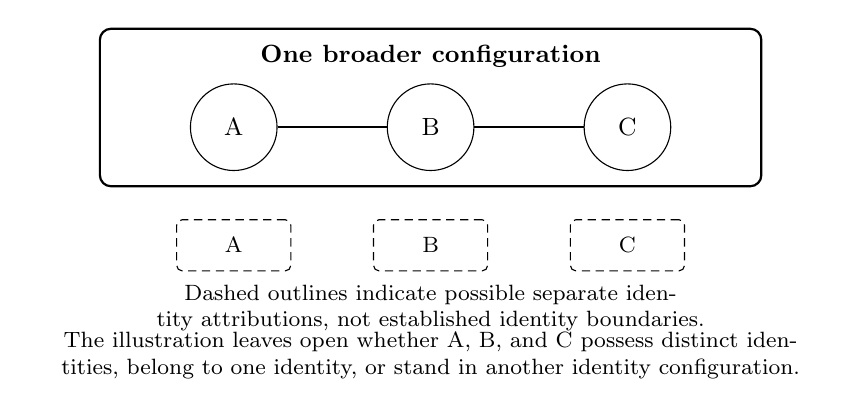
\begin{tikzpicture}[
    element/.style={
        circle,
        draw,
        minimum size=11mm,
        font=\small
    },
    possible/.style={
        draw,
        densely dashed,
        rounded corners=2pt,
        minimum width=1.45cm,
        minimum height=0.65cm,
        font=\footnotesize
    }
]

% Broader configuration
\draw[thick, rounded corners=4pt]
    (-4.2,1.0) rectangle (4.2,-1.0);

\node[font=\small\bfseries] at (0,0.65) {
    One broader configuration
};

% Elements within the configuration
\node[element] (a) at (-2.5,-0.25) {A};
\node[element] (b) at (0,-0.25) {B};
\node[element] (c) at (2.5,-0.25) {C};

\draw[thick] (a) -- (b);
\draw[thick] (b) -- (c);

% Possible identity attributions
\node[possible] at (-2.5,-1.75) {
    A
};

\node[possible] at (0,-1.75) {
    B
};

\node[possible] at (2.5,-1.75) {
    C
};

\node[
    align=center,
    text width=10cm,
    font=\footnotesize
] at (0,-2.55) {
    Dashed outlines indicate possible separate identity
    attributions, not established identity boundaries.
};

\node[
    align=center,
    text width=10cm,
    font=\footnotesize
] at (0,-3.15) {
    The illustration leaves open whether A, B, and C
    possess distinct identities, belong to one identity,
    or stand in another identity configuration.
};

\end{tikzpicture}

\caption{A unified configuration with identity attributions left open}
\label{fig:multiple-identity-attributions-within-one-configuration}

\end{figure}

% =============================================================================
% END OF ASSET IL01
% =============================================================================

The illustration provides a concrete way to consider
different possible attributions within one organized
configuration. It is illustrative rather than evidential:
it does not establish that the depicted elements possess
distinct identities, nor that the encompassing configuration
constitutes an additional identity. Those conclusions
would require independent ontological grounds.

% -----------------------------------------------------------------------------
\subsection{Plurality Without Premature Enumeration}

Even where identity plurality is established in a particular
case, its numerical structure requires further examination.
The recognition that more than one identity is involved
does not by itself determine the total number of identities,
their relations, or the principles by which they are
distinguished.

The identities involved need not be assumed to form
a collection of independent and mutually isolated units.
They may be related in ways that affect their constitution,
manifestation, or organization without necessarily
eliminating their distinction.

Likewise, the recognition of a broader configuration
does not automatically establish an additional identity
above or beyond the identities already distinguished.
A higher-order identity, if proposed, would require
its own ontological justification rather than being
inferred from the mere existence of a grouping or
composition.

For these reasons, identity plurality should not be
reduced to a numerical inventory made before the relevant
identity criteria have been clarified. Enumeration
presupposes that the units to be counted have already
been identified as identities. Where that prior
determination remains unsettled, a numerical conclusion
would merely restate the unresolved question.

% -----------------------------------------------------------------------------
\subsection{Conditions for a Responsible Attribution of Identity Plurality}

The preceding analysis indicates that an attribution
of identity plurality requires more than the observation
of multiplicity. At a minimum, an adequate account
must clarify the subject of the attribution, the respect
under which plurality is asserted, and the grounds
for distinguishing the identities involved.

It must also distinguish identity plurality from
manifestational, compositional, and relational multiplicity.
Where a common source or unified aggregate is relevant,
the account must explain precisely what follows from
that relation and what does not.

The requirements may be stated as follows:

\begin{enumerate}
    \item The entities or configurations to which identity
    is attributed must be specified.
    \item The respect and scope of the plurality claim
    must be made explicit.
    \item The grounds for distinguishing identities must
    be stated rather than inferred from difference alone.
    \item Relations among the identities must be examined
    without presuming that relation either eliminates
    or guarantees distinction.
    \item The attribution must not depend solely on the
    number of manifestations, components, relations,
    sources, or aggregates.
    \item The conclusion must remain proportionate to
    the grounds actually established.
\end{enumerate}

These requirements are methodological constraints on
ontological argument. They do not constitute a completed
definition of identity plurality, nor do they provide
a universal test that can be applied without regard
to the particular ontological problem.

Their function is to prevent unsupported transitions
from one kind of multiplicity to another and to make
explicit what an argument for identity plurality would
need to establish.

% -----------------------------------------------------------------------------
\subsection{Conclusion: Identity Plurality as an Open Ontological Problem}

Plurality of identities is a genuine ontological possibility
that cannot be excluded merely by appealing to the unity
of an existent, a common source, or a unified aggregate.
At the same time, it cannot be established merely by
counting components, manifestations, relations, or
differences between configurations.

The inquiry has therefore maintained the distinction
between identity plurality and other forms of multiplicity.
It has also shown that identity distinction requires
grounds that are relevant to identity itself. Similarity,
difference, spatial separation, material continuity,
structural integration, and relational connection may
be relevant to the analysis, but none independently
settles the question in every case.

No universal conclusion has been established here
that every existent possesses exactly one identity.
Nor has the universal attribution of multiple identities
been established. The number and organization of identities
must remain open wherever the relevant ontological
grounds have not been sufficiently determined.

The next section examines plurality and composition
more directly. It will consider the relation between
compositional organization and identity without assuming
that the plurality of components either entails or
excludes plurality of identities.

% =============================================================================
% END OF SECTION 04 OF CHAPTER 03
% =============================================================================

% ------------------------------------------------------------
% SECTION 05
% ------------------------------------------------------------

% =============================================================================
% Project : THE_PHILOSOPHY_OF_VIABILITY
% Book    : Book I — Ontology of Viability
% Book ID : VS.B01
%
% File    : 2_MAINMATTER/PART_I_IDENTITY_AND_MANIFESTATION/
%           CHAPTER_03_UNITY_AND_PLURALITY/sections/
%           section_05_plurality_and_composition.tex
%
% Section : Chapter 03, Section 05
% Title   : Plurality and Composition
%
% Purpose :
%   To examine the ontological relation between components,
%   compositional organization, wholes, and identity without
%   reducing identity to composition or inferring identity
%   plurality from component multiplicity.
%
% =============================================================================

\section{Plurality and Composition}
\label{sec:plurality-and-composition}

% -----------------------------------------------------------------------------
\subsection{The Ontological Problem of Composition}

Composition introduces a specific problem into the analysis
of unity and plurality. An existent may involve multiple
components that participate in an organized configuration.
The components may differ in their material constitution,
structural position, relations, determinations, or modes
of manifestation.

The presence of such components raises questions about
the ontological relation between the components and the
configuration in which they participate. It also raises
the question of whether the unity of that configuration
has implications for the identity attributed to it.

These questions must not be answered by counting components
alone. A plurality of components does not establish a
plurality of identities. Equally, the organization of
several components into one composition does not establish
that the composition possesses exactly one identity.

Composition and identity therefore require distinct
analyses. Their possible relation must be investigated
without presupposing that either the components or the
composed whole provide an exhaustive foundation for identity.

% -----------------------------------------------------------------------------
\subsection{Composition as an Organized Relation}

Composition is considered here as an ontological relation
through which multiple components participate in the
constitution of a more comprehensive configuration.
It is not merely the act of considering several elements
together, nor is every collection of elements necessarily
a composition in the relevant sense.

A composition may involve relations of arrangement,
organization, integration, dependence, or constitutive
participation. The specific relations involved determine
how the components belong to the configuration and how
their organization differs from an arbitrary grouping.

The concept of composition must nevertheless be distinguished
from the concept of identity. An organized composition
may be identifiable as a configuration under a specified
description without the ontological status of its identity
being settled.

Likewise, participation in a composition does not by itself
establish that a component loses every form of ontological
distinction. The components may remain differentiated
while participating in relations that constitute the whole.

Composition must therefore be examined as a relation
among constituents. It cannot be treated, without further
argument, as a complete explanation of the identity
of the resulting configuration.

% -----------------------------------------------------------------------------
\subsection{Plurality of Components and Plurality of Identities}

The plurality of components is not sufficient to establish
the plurality of identities. An existent may involve
several components while its identity remains unified
in a particular ontological respect. This possibility
blocks a direct inference from compositional multiplicity
to identity plurality.

The distinction can be expressed as follows:

\[
\text{Plurality of Components}
\not\Rightarrow
\text{Plurality of Identities}
\]

This expression does not establish that every composition
possesses one identity. It establishes only that the
number of components cannot serve as a direct measure
of the number of identities involved.

A component may participate in a composition without
being established as an independently distinct identity.
Conversely, a component may possess an identity that is
not reducible to its participation in the broader composition.
Whether either possibility obtains in a particular case
requires an independent ontological account.

The relation between components and identities must
therefore be examined without assuming a necessary
one-to-one correspondence.

% =============================================================================
% Project : THE_PHILOSOPHY_OF_VIABILITY
% Book    : Book I — Ontology of Viability
% Book ID : VS.B01
%
% File    : 4_ASSETS/tables/
%           VS.B01.P01.C03.S05.SS03.P012.TL01.components_composition_whole_and_identity.tex
%
% Asset   : TL01 — Components, Composition, Whole, and Identity
%
% Purpose :
%   To distinguish the principal ontological terms involved
%   in compositional analysis and to prevent unsupported
%   inferences from component multiplicity to identity.
%
% =============================================================================

\begin{table}[htbp]
\centering
\caption{Components, Composition, Whole, and Identity}
\label{tab:components-composition-whole-and-identity}

\small
\renewcommand{\arraystretch}{1.35}

\begin{tabular}{p{0.19\textwidth} p{0.34\textwidth} p{0.35\textwidth}}
\hline
\textbf{Term}
&
\textbf{Primary concern}
&
\textbf{What it does not establish by itself}
\\
\hline

Component
&
An element participating in a broader configuration.
&
That it possesses an independently distinct identity.
\\

Composition
&
The organized relations through which components
participate in a configuration.
&
That the resulting configuration possesses exactly
one identity.
\\

Aggregate
&
A plurality of elements considered together under
a grouping or unity criterion.
&
That the grouping constitutes a composition or
a distinct identity.
\\

Composed whole
&
A configuration considered through the organization
of its participating components.
&
That its identity is reducible to its components
or their arrangement.
\\

Structural organization
&
The positions and relations through which components
are organized.
&
That structural unity is equivalent to identity unity.
\\

Material constitution
&
The material elements and conditions involved
in the constitution of an existent.
&
That material continuity or integration determines
identity.
\\

Identity
&
The ontological unity or distinction attributable
at the level of identity.
&
That its status can be inferred solely from
component count or compositional organization.
\\

\hline
\end{tabular}

\end{table}

% =============================================================================
% END OF ASSET TL01
% =============================================================================

The table distinguishes the principal terms involved
in compositional analysis. It is not intended as an
exhaustive taxonomy. Its purpose is to prevent a conclusion
about identity from being inferred directly from a
description of components or their organization.

% -----------------------------------------------------------------------------
\subsection{Unity of Composition and Unity of Identity}

The unity of a composition does not automatically
establish the unity of identity. A composition may
exhibit extensive organization, structural integration,
or coordination among its components. These conditions
may warrant treating the components as one organized
configuration under a specified compositional respect.

Nevertheless, the unity of the configuration in that
respect does not settle whether its identity is singular,
plural, or related to the identities of its constituents
in another ontological manner.

The distinction can be expressed schematically:

\[
\text{Unity of Composition}
\not\Rightarrow
\text{Unity of Identity}
\]

This does not mean that composition is irrelevant to
identity. The organization of components may contribute
to conditions under which an identity is constituted,
maintained, or manifested. Such a contribution, however,
must be established rather than assumed.

The unity of composition and the unity of identity may
coincide in a particular existent. Their possible
coincidence does not make them conceptually equivalent,
nor does it establish a universal rule connecting them.

% -----------------------------------------------------------------------------
\subsection{Components and the Composed Whole}

The relation between components and a whole cannot
be adequately described through a simple opposition
between wholly independent parts and an entirely
self-contained whole.

Components may participate in the constitution of a
whole through relations that determine their arrangement,
dependence, and mutual contribution. At the same time,
the whole may possess determinations that cannot be
attributed to each component considered in isolation.

At least four possibilities require separate consideration:

\begin{enumerate}
    \item Components may retain distinct ontological
    determinations while participating in one composition.

    \item Components may acquire or enter into further
    determinations through their relations within
    a composition.

    \item The composed whole may exhibit determinations
    that are not attributable to the isolated components
    considered separately.

    \item The relation between components and whole may
    involve forms of dependence that cannot be described
    solely through spatial inclusion or material contact.
\end{enumerate}

These possibilities do not constitute a universal theory
of composition. They indicate that the relation between
components and whole must be examined through its
specific ontological conditions.

No conclusion about identity follows from the mere
presence of any one of these relations. In particular,
the attribution of a determination to the whole does
not automatically establish an additional identity,
and the distinction of a component does not automatically
establish an independent identity.

% -----------------------------------------------------------------------------
\subsection{Composition Without Homogeneity}

The formation of a composition does not necessarily
eliminate differences among its components. Components
may remain differentiated in their material, structural,
relational, or functional determinations while participating
in an organized whole.

Compositional unity therefore need not be understood
as the reduction of components to homogeneity. A whole
may be organized through differentiated contributions,
and the differences among its components may be relevant
to the organization of the composition.

Conversely, the preservation of differences among
components does not automatically negate the unity
of the composition. Difference and compositional unity
are not mutually exclusive in every respect.

This point must not, however, be transferred without
qualification to identity. The compatibility of internal
difference with compositional unity does not prove
identity unity. Whether differentiated components
belong to one identity or involve several identities
remains a distinct question.

% -----------------------------------------------------------------------------
\subsection{Composition and Material Constitution}

Material constitution may provide important conditions
for compositional relations. An existent may be constituted
through multiple material elements whose arrangement
and interaction contribute to its structure and
manifestation.

Material composition cannot, however, be treated as
an exhaustive definition of identity. The material
constituents of an existent may change while some
relevant ontological determinations remain preserved.
Conversely, the preservation of material constituents
does not by itself establish the preservation of identity.

Material continuity, material similarity, and material
integration are therefore insufficient as universal
criteria of identity unity or plurality. Their relevance
depends on the specific ontological question being examined.

This restriction does not imply that material constitution
is ontologically irrelevant. It means that the material
conditions of an existent must be distinguished from
the identity attributed to it. The significance of
material manifestation must be preserved without
reducing identity to material composition.

% -----------------------------------------------------------------------------
\subsection{Composition and Structural Organization}

Composition may involve structural organization through
which components occupy determinate positions and
participate in relations that constitute a configuration.
Such organization may distinguish one composition
from another and may be relevant to the conditions
under which a whole is constituted.

Structural distinction does not automatically establish
identity distinction. Two compositions may differ
structurally without that difference alone determining
whether they possess distinct identities. Conversely,
structural similarity does not establish that two
compositions share one identity.

Structural integration also cannot serve as a sufficient
criterion of identity unity. The fact that components
form a highly integrated structure does not establish,
without further argument, that the resulting whole
possesses only one identity.

The relation between composition and structure must
therefore be distinguished from the relation between
composition and identity. Structural organization
may be relevant to identity, but it cannot be treated
as an exhaustive substitute for identity itself.

% =============================================================================
% Project : THE_PHILOSOPHY_OF_VIABILITY
% Book    : Book I — Ontology of Viability
% Book ID : VS.B01
%
% File    : 4_ASSETS/diagrams/
%           VS.B01.P01.C03.S05.SS08.P032.DG01.components_composition_and_identity_relations.tex
%
% Asset   : DG01 — Components, Composition, and Identity Relations
%
% Purpose :
%   To represent the distinction between component plurality,
%   compositional organization, and identity without implying
%   that any one of these necessarily entails another.
%
% Requires (preamble):
%   \usepackage{tikz}
%   \usetikzlibrary{calc, positioning, fit}
% =============================================================================

\begin{figure}[htbp]
    \centering
    \hyphenpenalty=10000 \exhyphenpenalty=10000\relax  % no hyphenation inside diagram labels

    \begin{tikzpicture}[
        font=\small,
        node distance=0.4cm,
        % --- base box ---
        box/.style={
            draw, rounded corners=3pt, align=center,
            inner sep=6pt, line width=0.7pt
        },
        % --- node roles ---
        compbox/.style={box, text width=2.6cm, minimum height=1.1cm,
                        fill=blue!8, draw=blue!55!black},
        compositionbox/.style={box, text width=6.8cm, minimum height=1.5cm,
                               fill=blue!16, draw=blue!55!black},
        identitybox/.style={box, text width=6.8cm, minimum height=1.5cm,
                            dashed, fill=gray!10, draw=black!60},
        % --- frames and labels ---
        vsgroup/.style={draw=black!45, dashed, rounded corners=5pt,
                        inner sep=8pt, line width=0.5pt},
        grouplabel/.style={font=\footnotesize\itshape, text=black!75,
                           align=left},
        legendtext/.style={font=\scriptsize},
        % --- undirected lines (no arrowheads: no entailment, no priority) ---
        vsrel/.style={draw=black!70, line width=0.8pt},
        vslink/.style={draw=black!55, dashed, line width=0.7pt}
    ]

    % ---------------------------------------------------------------
    % Components (equal rank)
    % ---------------------------------------------------------------
    \node[compbox] (b) {Component B};
    \node[compbox, left=of b]  (a) {Component A};
    \node[compbox, right=of b] (c) {Component C};

    \node[vsgroup, fit=(a)(b)(c)] (comps) {};
    \node[grouplabel, anchor=south west] at (comps.north west) {
        Component plurality
    };

    % ---------------------------------------------------------------
    % Composition and identity
    % ---------------------------------------------------------------
    \node[compositionbox, below=1.1cm of comps] (whole) {
        \textbf{Composition}\\[3pt]
        Organized relations among components
    };
    \node[identitybox, below=1.1cm of whole] (id) {
        \textbf{Identity}\\[3pt]
        Unity or plurality requires identity-level grounds
    };

    % each component participates in the composition (straight, vertical)
    \draw[vsrel] (a.south) -- (a.south |- whole.north);
    \draw[vsrel] (b.south) -- (b.south |- whole.north);
    \draw[vsrel] (c.south) -- (c.south |- whole.north);

    % possible ontological relevance (not entailment)
    \draw[vslink] (whole) -- (id);

    % ---------------------------------------------------------------
    % Legend and interpretive constraint
    % ---------------------------------------------------------------
    \node[below=0.7cm of id, legendtext] (legend) {
        \tikz[baseline=-0.5ex]\draw[vsrel] (0,0) -- (0.6,0);~participation in an organized configuration
        \quad\quad
        \tikz[baseline=-0.5ex]\draw[vslink] (0,0) -- (0.6,0);~possible ontological relevance
    };

    \node[below=0.4cm of legend, text width=10.5cm, align=center,
          font=\footnotesize\itshape] {
        \textbf{Interpretive constraint:}
        The component-to-composition connections represent
        participation in an organized configuration. The
        composition-to-identity connection represents possible
        ontological relevance, not entailment. Component count
        and compositional unity do not determine identity number.
    };

    \end{tikzpicture}

    \caption{The distinct relations among components, composition, and identity}
    \label{fig:components-composition-and-identity-relations}
\end{figure}

% =============================================================================
% END OF ASSET DG01
% =============================================================================


The diagram distinguishes the relations among components,
composition, and identity. Its connections indicate
possible ontological relevance, not necessary entailment
or a fixed sequence of constitution.

% -----------------------------------------------------------------------------
\subsection{The Possibility of Multiple Identities Within a Composition}

The unity of a composition does not exclude the possibility
that multiple identities may be involved within it.
An organized whole may include components or subsystems
whose identity relations require independent examination.

However, the presence of differentiated components
or subsystems does not automatically establish that
each possesses a distinct identity. Such an attribution
requires grounds relevant to identity itself rather than
an inference from structural or functional differentiation.

A composition may therefore involve several determinations
at once: unity of composition, plurality of components,
differentiation of structural relations, and a possible
unity or plurality of identities. These determinations
concern different ontological respects and are not
contradictory merely because they coexist.

The possibility of multiple identities within a composition
must remain open. It must not be treated as an automatic
consequence of compositional multiplicity, nor excluded
by appealing to the unity of the composed whole.

% -----------------------------------------------------------------------------
\subsection{One Identity Across Compositional Transformation}

The relation between composition and identity also raises
the question of whether one identity may be associated
with different compositional configurations.

A composition may undergo changes in its components,
their arrangement, or their relations. Such changes
do not automatically establish the emergence of a new
identity. Nor does the preservation of a particular
composition automatically establish that the same
identity persists.

A reduction of identity to composition would tend to
treat every identity-relevant compositional change as
an identity change. An account that entirely separates
identity from composition, on the other hand, would
risk ignoring the possible constitutive significance
of compositional conditions.

Neither position can be accepted without further argument.
The relation must be examined in terms of the specific
conditions under which composition contributes to
identity constitution, manifestation, or distinction.

This inquiry must also distinguish compositional
transformation from identity persistence. The former
describes a change in the organization or constituents
of a composition; the latter concerns whether an identity
continues to obtain. One cannot be used as a substitute
for the other.

% -----------------------------------------------------------------------------
\subsection{Composition, Aggregate, and Identity}

Composition, aggregate, and identity must remain
conceptually distinct. An aggregate concerns a plurality
of elements considered together under some grouping
or unity criterion. A composition concerns relations
through which components participate in an organized
configuration. Identity concerns the ontological unity
or distinction attributable at the level of identity.

These concepts may refer to related aspects of an
existent, but they answer different questions. The
distinction can be summarized as follows:

\[
\begin{aligned}
\text{Aggregate} &\neq \text{Composition}
\\
\text{Composition} &\neq \text{Identity}
\\
\text{Unity of Composition} &\neq \text{Unity of Identity}
\\
\text{Plurality of Components} &\neq
\text{Plurality of Identities}
\end{aligned}
\]

The distinction between aggregate and composition
does not imply that every aggregate is wholly unorganized
or that every composition possesses a particular degree
of integration. It indicates that the relations through
which a whole is constituted must be specified before
conclusions about its ontological unity are drawn.

Similarly, the distinction between composition and
identity does not imply that identity is independent
of every compositional condition. It prevents composition
from being treated as sufficient, by itself, to determine
identity.

% -----------------------------------------------------------------------------
\subsection{The Limits of Compositional Reduction}

Compositional reduction occurs when identity is explained
entirely through components and their organization.
Such an account may provide important information
about the constitution of an existent, but it risks
assuming that a complete description of composition
is equivalent to a complete account of identity.

A description of components and their relations may
explain how a configuration is organized without
settling the ontological question of what identity
belongs to that configuration. The identification
of a composition is not yet an explanation of the
identity attributed to it.

The opposite reduction must also be avoided. Treating
identity as wholly independent of composition would
be premature where compositional conditions may
contribute to identity constitution, manifestation,
or distinction.

The appropriate position is therefore neither to
identify identity with composition nor to deny every
ontological relevance of composition. Composition
may be one dimension of the conditions relevant to
identity. Whether it constitutes, constrains, or
merely accompanies a particular identity relation
must be established through further analysis.

% -----------------------------------------------------------------------------
\subsection{Illustrative Case: Components and an Organized Configuration}

Consider a device assembled from several components.
The components may be distinguishable, replaceable,
or organized in different ways. Their arrangement
may constitute a functioning configuration, but the
mere fact that they form one assembled device does
not settle every question concerning identity.

The components may be considered individually, the
assembled configuration may be considered as a whole,
and the relations among the components may be examined
as a compositional organization. These are different
objects of analysis, even when they concern the same
concrete case.

% =============================================================================
% Project : THE_PHILOSOPHY_OF_VIABILITY
% Book    : Book I — Ontology of Viability
% Book ID : VS.B01
%
% File    : 4_ASSETS/illustrations/
%           VS.B01.P01.C03.S05.SS13.P047.IL01.components_and_composed_configuration.tex
%
% Asset   : IL01 — Components and Composed Configuration
%
% Purpose :
%   To illustrate the difference between distinguishable
%   components and their organization as a composed whole,
%   while leaving identity attribution unresolved.
%
% =============================================================================

\begin{figure}[htbp]
\centering

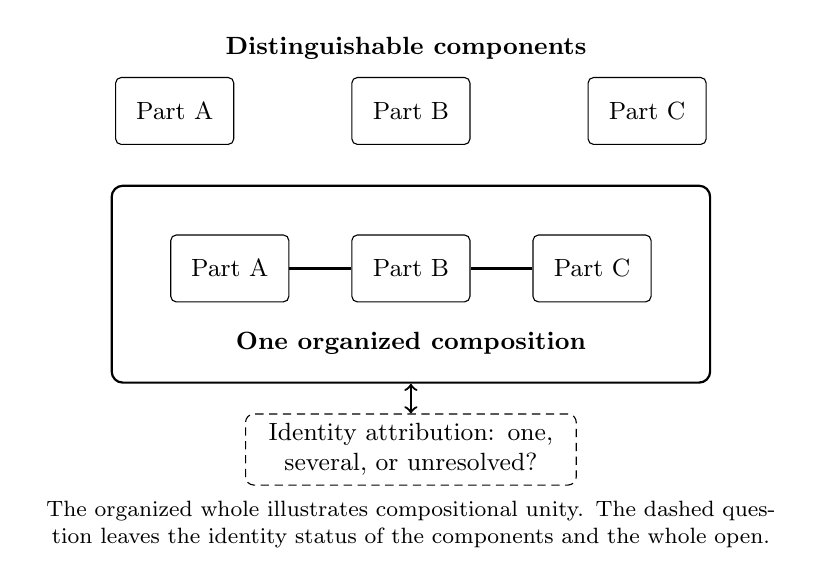
\begin{tikzpicture}[
    part/.style={
        draw,
        rounded corners=2pt,
        minimum width=1.5cm,
        minimum height=0.85cm,
        align=center,
        font=\small
    },
    whole/.style={
        draw,
        rounded corners=4pt,
        thick,
        minimum width=7.6cm,
        minimum height=2.5cm
    },
    question/.style={
        draw,
        densely dashed,
        rounded corners=3pt,
        minimum width=4.2cm,
        minimum height=0.9cm,
        align=center,
        text width=3.9cm,
        font=\small
    }
]

% Components considered separately
\node[part] (p1) at (-3.0,1.2) {Part A};
\node[part] (p2) at (0,1.2) {Part B};
\node[part] (p3) at (3.0,1.2) {Part C};

\node[align=center, font=\small\bfseries] at (0,2.0) {
    Distinguishable components
};

% Composed configuration
\node[whole] (frame) at (0,-1.0) {};

\node[part] (a) at (-2.3,-0.8) {Part A};
\node[part] (b) at (0,-0.8) {Part B};
\node[part] (c) at (2.3,-0.8) {Part C};

\draw[thick] (a) -- (b);
\draw[thick] (b) -- (c);

\node[font=\small\bfseries] at (0,-1.75) {
    One organized composition
};

% Identity question
\node[question] (identity) at (0,-3.1) {
    Identity attribution:
    one, several, or unresolved?
};

\draw[<->, thick] (frame.south) -- (identity.north);

\node[
    align=center,
    text width=9.5cm,
    font=\footnotesize
] at (0,-4.05) {
    The organized whole illustrates compositional unity.
    The dashed question leaves the identity status of
    the components and the whole open.
};

\end{tikzpicture}

\caption{Distinguishable components organized within one composition}
\label{fig:components-and-composed-configuration}

\end{figure}

% =============================================================================
% END OF ASSET IL01
% =============================================================================

The illustration is intended to clarify the distinction
between component multiplicity and compositional unity.
It does not establish whether the components or the
assembled configuration possess distinct identities.
Nor does it establish that the assembled whole constitutes
an additional identity. Those conclusions require
independent ontological grounds.

% -----------------------------------------------------------------------------
\subsection{The Relation to Unity and Plurality}

The analysis of composition clarifies that unity and
plurality cannot be attributed to an existent without
specifying their subject and respect. A composition
may be unified with respect to its organization while
remaining plural with respect to its components.

The same configuration may also raise questions of
identity unity or plurality that are not settled by
either of those descriptions. The unity of composition
and the plurality of components may coexist without
contradiction because they concern different
ontological determinations.

The relevant distinctions include:

\begin{itemize}
    \item Unity of composition and plurality of components.
    \item Unity of an aggregate and plurality of its constituents.
    \item Unity of identity and plurality of determinations.
    \item Unity of a broader configuration and possible
    plurality of identities.
\end{itemize}

These relations must not be collapsed into a single
opposition between the one and the many. The question
is not simply whether an existent is one or many. It
is necessary to determine what is one, what is many,
and whether the relevant claims concern components,
composition, aggregate, manifestation, or identity.

% -----------------------------------------------------------------------------
\subsection{Conclusion: Composition as Relevant but Non-Exclusive}

Composition is an important ontological dimension
in the examination of unity and plurality. It concerns
the relations through which multiple components
participate in an organized configuration.

Neither the plurality of components nor the unity
of their composition is sufficient, by itself, to
establish the plurality or unity of identity. Composition
may contribute to the conditions under which identity
is constituted or manifested, but it cannot be treated
as the exclusive foundation of identity.

Likewise, identity cannot be considered independent
of every compositional condition without further
argument. The ontological relation between composition
and identity must therefore be examined without
reducing either to the other.

The next section turns to the broader relation between
identity and multiplicity. It considers the different
forms of multiplicity that may occur within an existent
or across a plurality of existents, and examines why
multiplicity cannot be treated as synonymous with
plurality of identities.

% =============================================================================
% END OF SECTION 05 OF CHAPTER 03
% =============================================================================

% ------------------------------------------------------------
% SECTION 06
% ------------------------------------------------------------

% =============================================================================
% Section 06 — Identity and Multiplicity
% Book I — Ontology of Viability
% Chapter 03 — Unity and Plurality
%
% Purpose:
%   To distinguish multiplicity in its general ontological
%   sense from plurality of identities, and to examine
%   the different forms of multiplicity that may occur
%   within and across existents.
%
% Conceptual Policy:
%   1. Multiplicity is broader than plurality of identities.
%   2. Multiplicity of determinations, manifestations,
%      components, or relations does not automatically
%      establish identity plurality.
%   3. Unity of identity does not require the elimination
%      of every form of multiplicity.
%   4. Identity must not be reduced to a numerical count
%      of multiple elements.
%   5. The ontological subject and respect of every
%      multiplicity claim must be specified.
%   6. Neither universal identity unity nor universal
%      identity plurality is presupposed.
%
% =============================================================================

\section{Identity and Multiplicity}
\label{sec:identity-and-multiplicity}

% -----------------------------------------------------------------------------
\subsection{The Ontological Problem of Multiplicity}

Multiplicity is a broad ontological determination
that may occur in different forms and at different
levels of an existent or a configuration of existents.

An existent may involve multiple determinations,
components, relations, manifestations, processes,
or compositional elements.

A plurality of existents may also participate
in a broader configuration in which their relations
produce further forms of multiplicity.

However, the recognition of multiplicity does not
by itself settle the question of identity.

Multiplicity and plurality of identities are
not equivalent concepts.

The former concerns the presence of more than
one element, determination, or relation in
a specified ontological respect.

The latter concerns the existence of more than
one identity.

The distinction is essential because multiplicity
may occur without identity plurality being
established.

Conversely, identity plurality may involve
relations and forms of organization that cannot
be adequately described through a simple
enumeration of elements.

The present section examines this distinction
and establishes the conceptual conditions
necessary for discussing multiplicity without
reducing identity to it.

% -----------------------------------------------------------------------------
\subsection{Multiplicity as a General Ontological Determination}

Multiplicity refers to the presence or constitution
of more than one element, determination, relation,
or manifestation within a specified ontological
domain or respect.

Its meaning depends on what is being considered
multiple.

Multiplicity may concern:

\begin{itemize}
    \item Components of an existent.
    \item Determinations belonging to an existent.
    \item Relations in which an existent participates.
    \item Manifestations associated with an existent.
    \item Processes or transformations involving
    an existent.
    \item Existents participating in a broader
    configuration.
\end{itemize}

These forms of multiplicity are not identical.

A plurality of components concerns compositional
multiplicity.

A plurality of determinations concerns the
differentiation of what characterizes an existent.

A plurality of relations concerns the multiplicity
of relational connections.

A plurality of manifestations concerns the
multiplicity of ways in which an existent
is manifested.

Each form requires its own ontological analysis.

The general concept of multiplicity therefore
cannot be treated as a single undifferentiated
category.

More importantly, none of these forms can
automatically be transferred into a conclusion
about the number of identities involved.

% -----------------------------------------------------------------------------
\subsection{Multiplicity and the Subject of Multiplicity}

Every claim of multiplicity requires the
identification of its subject.

To say that something is multiple is incomplete
unless it is specified what is being considered
multiple.

The subject may be an existent, a composition,
a set of determinations, a relational configuration,
a manifestation, or identity itself.

These subjects cannot be treated as interchangeable.

For example, an existent may be multiple in
its components while unified in another respect.

It may also exhibit several manifestations
without the identity relation among those
manifestations being determined.

Similarly, a plurality of existents may form
one aggregate without thereby constituting
one identity.

The subject of multiplicity must therefore
be distinguished from the subject of identity.

This requirement prevents the transfer of
a numerical description from one ontological
domain to another without justification.

A multiplicity claim must consequently specify:

\begin{enumerate}
    \item What is considered multiple.
    \item The domain in which multiplicity occurs.
    \item The ontological respect under consideration.
    \item The relation, if any, between that
    multiplicity and identity.
\end{enumerate}

Without these distinctions, the term multiplicity
risks becoming too broad to support precise
ontological conclusions.

% -----------------------------------------------------------------------------
\subsection{Multiplicity Does Not Necessarily Imply Identity Plurality}

The central distinction of this section is that
multiplicity does not necessarily imply plurality
of identities.

An existent may involve numerous components,
determinations, relations, or manifestations
without this multiplicity automatically
establishing more than one identity.

The relation can be expressed as follows:

\[
\text{Multiplicity}
\not\Rightarrow
\text{Plurality of Identities}
\]

This expression does not establish that
multiplicity and identity plurality are
unrelated.

It establishes that the former is not
a sufficient condition for the latter.

The presence of multiple elements may be
relevant to an investigation of identity,
but the ontological significance of those
elements must be independently demonstrated.

For example, the plurality of components
within a composition does not by itself
establish that each component possesses
a distinct identity.

Likewise, the plurality of manifestations
associated with an existent does not
establish that each manifestation constitutes
a separate identity.

The inference from multiplicity to identity
plurality therefore requires an additional
account of identity distinction.

Without such an account, the inference
remains unsupported.

% -----------------------------------------------------------------------------
\subsection{Identity Unity Does Not Require the Elimination of Multiplicity}

The distinction must also be maintained
in the opposite direction.

The unity of identity does not necessarily
require the absence of multiplicity.

An existent may involve multiple determinations,
components, relations, or manifestations
while its identity remains unified in
a particular ontological respect.

Unity of identity therefore cannot be defined
simply as the elimination of multiplicity.

Such a definition would confuse unity with
homogeneity or numerical indivisibility.

It would also impose an unnecessary opposition
between identity unity and internal differentiation.

The presence of multiplicity may be compatible
with unity, but this compatibility does not
mean that every multiplicity is necessarily
contained within one identity.

The relevant question is whether the multiplicity
under consideration belongs to the constitution,
manifestation, or relations of one identity,
or whether it involves a plurality of identities.

That question cannot be settled by the mere
recognition of multiplicity.

The distinction must be established through
an examination of the ontological subject
and the relations involved.

% -----------------------------------------------------------------------------
\subsection{Multiplicity of Determinations}

An existent may possess multiple determinations
that distinguish different aspects of its
ontological constitution.

These determinations may concern different
domains, relations, modes, or conditions
of existence.

Their plurality does not automatically imply
that the existent possesses multiple identities.

A plurality of determinations may be compatible
with the unity of identity.

However, this possibility must not be turned
into the assumption that all determinations
necessarily belong to one identity.

The relation between determinations and identity
requires an account of how determinations
participate in the constitution or distinction
of identity.

A determination may be relevant to identity
without being identical to identity.

Likewise, the plurality of determinations
may contribute to the differentiation of
an existent without establishing identity
plurality.

The distinction between identity and its
determinations must therefore be preserved.

This also prevents identity from being reduced
to a list or aggregate of features.

An inventory of determinations may describe
an existent, but it does not by itself
provide an exhaustive account of its identity.

% -----------------------------------------------------------------------------
\subsection{Multiplicity of Manifestations}

Multiplicity may also occur at the level
of manifestation.

An existent may manifest through different
configurations, forms, or modes.

These manifestations may be related to
one another in different ways.

They may exhibit continuity, transformation,
difference, or other forms of ontological
relation.

However, the multiplicity of manifestations
does not automatically determine whether
one identity or multiple identities are involved.

A plurality of manifestations may be associated
with one identity, but this cannot be assumed
as a universal rule.

Likewise, distinct manifestations may involve
distinct identities, but their difference
does not establish that conclusion by itself.

The relation between manifestation and identity
must therefore be examined without imposing
a direct numerical correspondence.

This distinction is particularly important
when an existent undergoes transformation.

A change in manifestation does not automatically
establish a change in identity.

Nor does the preservation of a recognizable
manifestational configuration automatically
establish identity continuity.

The relevant ontological relations require
independent analysis.

% -----------------------------------------------------------------------------
\subsection{Multiplicity of Relations}

An existent may participate in multiple
relations with other existents or with
different ontological domains.

These relations may differ in their nature,
scope, direction, or significance.

Relational multiplicity does not automatically
establish plurality of identities.

One identity may be involved in multiple
relations without thereby becoming multiple.

Conversely, the unity of a relational subject
does not automatically exclude the possibility
that a broader configuration involves
multiple identities.

The number of relations and the number
of identities therefore concern different
ontological questions.

A relational configuration may also involve
relations among several identities, but
this possibility must be established through
the ontological distinction of the related
subjects.

It cannot be inferred merely from the
multiplicity of relational connections.

The analysis must therefore distinguish
relational multiplicity from identity plurality
while preserving the possibility that
relations may be relevant to identity
constitution and distinction.

% -----------------------------------------------------------------------------
\subsection{Multiplicity of Processes and Transformations}

Multiplicity may also concern processes
and transformations.

An existent may undergo several transformations
or participate in multiple processes
throughout its existence.

Such multiplicity may involve changes
in determinations, structure, composition,
relations, or manifestation.

However, the plurality of transformations
does not automatically establish plurality
of identities.

Nor does the existence of multiple processes
necessarily indicate that one identity
is involved.

A process may be associated with one identity,
with several identities, or with a configuration
whose identity relations remain undetermined.

The ontological status of the process and
the identity of the existent must therefore
be examined separately.

This distinction also prevents the reduction
of identity to a sequence of states or events.

A temporal or processual description may
provide relevant information about an existent,
but it does not by itself settle the question
of identity unity or plurality.

% -----------------------------------------------------------------------------
\subsection{Multiplicity Across Different Ontological Respects}

Multiplicity may be present in one ontological
respect while unity is present in another.

An existent may be materially composite,
structurally organized, relationally differentiated,
and unified in some other respect.

These descriptions need not contradict one another
because they concern different determinations.

The same applies to plurality of existents.

Several existents may constitute one aggregate
in a compositional respect while remaining
distinct in their identities.

Likewise, multiple manifestations may be
related through one source without their
identity relations being settled.

The distinction between different respects
prevents unity and plurality from being
treated as mutually exclusive descriptions
in every case.

The ontological question must instead determine
whether the relevant claims concern the same
subject and the same respect.

Only when they concern the same subject
under the same respect does an apparent
opposition require further resolution.

The following schematic expressions illustrate
the distinction:

\[
\begin{aligned}
&\text{Unity of Identity}
\quad+\quad
\text{Multiplicity of Determinations}
\\[4pt]
&\text{Unity of Composition}
\quad+\quad
\text{Multiplicity of Components}
\\[4pt]
&\text{Unity of Source}
\quad+\quad
\text{Multiplicity of Manifestations}
\end{aligned}
\]

These expressions indicate possible combinations
of unity and multiplicity across different
ontological respects.

They do not establish that every such combination
necessarily occurs in every existent.

% -----------------------------------------------------------------------------
\subsection{Multiplicity and the Problem of Ontological Levels}

The examination of multiplicity also requires
attention to the ontological level at which
a plurality is attributed.

A plurality may concern elements within
an existent, relations among existents,
or a broader configuration in which multiple
existents participate.

These levels must not be collapsed.

For example, the multiplicity of components
within one composition is not equivalent
to the plurality of existents participating
in a larger configuration.

Likewise, the plurality of existents within
a configuration does not automatically
establish plurality of identities at every
level of that configuration.

The ontological relation between levels
requires separate analysis.

A broader whole may involve relations among
multiple existents without necessarily
constituting a new identity.

Conversely, the possibility of a broader
identity cannot be rejected merely because
the whole contains multiple existents.

The relation between levels of organization
and identity therefore remains an open
ontological problem.

It cannot be resolved by assuming that
identity is always located at the level
of the smallest component or the largest
configuration.

% -----------------------------------------------------------------------------
\subsection{Multiplicity and Numerical Enumeration}

Numerical enumeration may be useful for
describing multiplicity.

It may establish that a specified domain
contains several components, manifestations,
relations, or existents.

However, numerical enumeration alone
does not establish the ontological nature
of the entities being counted.

Counting components does not determine
the number of identities.

Counting manifestations does not determine
the number of identities.

Counting relations does not determine
the number of identities.

The numerical result depends on the
ontological classification of what is
being counted.

If the counted elements are components,
the result concerns component plurality.

If they are manifestations, the result
concerns manifestational plurality.

If they are identities, the result concerns
identity plurality.

The category of enumeration must therefore
be established before numerical conclusions
are transferred to identity.

This prevents the use of numerical unity
or plurality as a substitute for ontological
analysis.

% -----------------------------------------------------------------------------
\subsection{The Relation Between Multiplicity and Difference}

Multiplicity is related to difference,
but the two concepts are not identical.

Multiplicity concerns the presence of more
than one element or determination in
a specified respect.

Difference concerns the distinction between
determinations, elements, or entities.

A plurality may include elements that are
similar in some respects and different
in others.

Likewise, difference may occur within
one existent without establishing plurality
of identities.

The presence of difference therefore does
not automatically establish identity plurality.

Conversely, the existence of multiple identities
does not require that they differ in every
possible determination.

Distinct identities may share determinations
or exhibit similarities without thereby
becoming one identity.

The relation between difference and identity
must therefore be examined independently
of numerical multiplicity.

This distinction is necessary to prevent
both the reduction of identity to similarity
and the reduction of plurality to difference
of appearance.

% -----------------------------------------------------------------------------
\subsection{The Limits of Multiplicity-Based Explanations of Identity}

Multiplicity-based explanations of identity
risk treating the number or arrangement
of elements as sufficient to determine
the identity of an existent.

Such explanations may describe important
features of composition, manifestation,
or relational organization.

However, they do not necessarily explain
why a particular identity is ontologically
unified or distinct.

A complete account of identity cannot
be replaced by an inventory of multiple
determinations.

Nor can identity plurality be established
by merely identifying several components
or manifestations.

The analysis must explain the ontological
relation between multiplicity and identity.

This requires a distinction between:

\begin{enumerate}
    \item Multiplicity as a condition or
    determination of an existent.

    \item Identity as an ontological
    determination of that existent.

    \item Plurality as a possible relation
    among identities.

    \item The relations through which
    multiplicity and identity may be connected.
\end{enumerate}

These distinctions do not imply that identity
and multiplicity are unrelated.

They prevent the assumption that one can
be fully explained through the other.

% -----------------------------------------------------------------------------
\subsection{Conclusion: Multiplicity Does Not Decide Identity}

Multiplicity is a broad ontological
determination that may occur in components,
determinations, relations, manifestations,
processes, and configurations.

Plurality of identities is a more specific
ontological claim concerning the existence
of more than one identity.

The two concepts must therefore remain distinct.

Multiplicity does not automatically establish
identity plurality.

Likewise, unity of identity does not require
the elimination of every form of multiplicity.

Unity and multiplicity may coexist when
they concern different ontological respects,
but their relation must be examined rather
than assumed.

The central methodological requirement
is to specify the subject, domain, and
respect of every claim of unity or plurality.

The next section examines the non-equivalence
of unity and singularity.

It considers why unity cannot be reduced
to numerical oneness and why numerical
singularity cannot serve as a complete
ontological explanation of identity.

% =============================================================================
% End of Section 06
% =============================================================================

% ------------------------------------------------------------
% SECTION 07
% ------------------------------------------------------------

% =============================================================================
% Section 07 — Non-Equivalence of Unity and Singularity
% Book I — Ontology of Viability
% Chapter 03 — Unity and Plurality
%
% Purpose:
%   To establish the ontological distinction between unity
%   and numerical singularity, and to examine why neither
%   concept can be reduced to the other.
%
% Conceptual Policy:
%   1. Unity is not equivalent to numerical singularity.
%   2. Numerical oneness does not establish unity of identity.
%   3. Unity does not necessarily imply the existence
%      of exactly one identity.
%   4. Plurality does not necessarily negate unity.
%   5. Unity must not be reduced to indivisibility,
%      homogeneity, or numerical oneness.
%   6. No universal conclusion concerning the number
%      of identities is adopted.
%
% =============================================================================

\section{Non-Equivalence of Unity and Singularity}
\label{sec:non-equivalence-of-unity-and-singularity}

% -----------------------------------------------------------------------------
\subsection{The Problem of Equating Unity with Singularity}

Unity and singularity are frequently treated as
equivalent determinations.

When something is described as one, it may be assumed
that it is singular in every relevant ontological
respect. Conversely, when something is described
as multiple, it may be assumed that unity is absent.

Such assumptions introduce a conceptual reduction
that must be examined.

Unity concerns the ontological determination through
which something is considered unified in a specified
respect.

Singularity, in its numerical sense, concerns
the condition of being one rather than more than
one within a particular domain of enumeration.

These concepts may coincide in particular cases,
but their possible coincidence does not establish
their equivalence.

The question is therefore not whether unity and
singularity can occur together.

It is whether one can be defined, established,
or inferred solely through the other.

The present section argues that such a reduction
is not ontologically justified.

% -----------------------------------------------------------------------------
\subsection{Unity as Distinct from Numerical Oneness}

Unity cannot be defined simply as numerical oneness.

Numerical oneness indicates that something is
counted as one within a specified domain and
under a particular criterion of enumeration.

Unity, however, concerns the ontological respect
in which something is considered unified.

The difference is important because numerical
counting presupposes that the subject of counting
and the criterion of individuation have already
been sufficiently determined.

It does not independently establish the ontological
unity of what is counted.

For example, an existent may be counted as one
object within a particular classification while
the unity of its identity remains an independent
ontological question.

Likewise, a system may be treated as one unit
for a particular practical or analytical purpose
without this designation establishing that
it possesses exactly one identity.

The numerical designation of one therefore
cannot replace an account of unity.

The following distinction must be maintained:

\[
\text{Numerical Oneness}
\neq
\text{Ontological Unity}
\]

This distinction does not deny that numerical
oneness may be relevant to the examination
of unity.

It denies that numerical oneness is sufficient
to establish it.

% -----------------------------------------------------------------------------
\subsection{Singularity as a Determination of Number}

Singularity concerns the numerical determination
of a subject as one within a specified domain
of counting.

Such a determination depends on what is being
counted and on the criterion through which
the counted subject is distinguished.

An existent may be considered singular as
a material object, a system, an organism,
or a bounded configuration.

However, these numerical descriptions do not
necessarily settle the question of identity.

The same existent may be singular under one
criterion of enumeration while involving
a plurality of components, relations,
or manifestations.

Likewise, several entities may be counted
as distinct units without this counting
establishing the ontological nature of their
identities.

Singularity is therefore meaningful only
in relation to a specified subject and
a specified numerical domain.

It cannot be treated as an unrestricted
ontological determination that automatically
applies to every aspect of an existent.

% -----------------------------------------------------------------------------
\subsection{The Difference Between Unity and Indivisibility}

Unity must also be distinguished from
indivisibility.

Indivisibility concerns whether something
can be divided into parts or whether such
division is possible under a specified
criterion.

Unity concerns the ontological respect
in which something is unified.

An existent may be divisible into components
while remaining unified in another respect.

Conversely, something may be treated as
indivisible within a particular analysis
without this establishing the unity of
its identity.

The possibility of division does not
automatically negate unity.

Nor does the absence of an identified
division establish unity.

The distinction can be expressed as follows:

\[
\text{Divisibility}
\not\Rightarrow
\text{Absence of Unity}
\]

and

\[
\text{Indivisibility}
\not\Rightarrow
\text{Unity of Identity}
\]

These expressions prevent the reduction
of unity to the absence of internal parts.

A theory of unity must therefore explain
the relevant ontological relation rather
than rely exclusively on criteria of
division or indivisibility.

% -----------------------------------------------------------------------------
\subsection{The Difference Between Unity and Homogeneity}

Unity is not equivalent to homogeneity.

Homogeneity concerns similarity or sameness
among elements or determinations in a
specified respect.

Unity concerns the ontological unity
attributable to a subject.

An existent may involve heterogeneous
components or differentiated determinations
while remaining unified in a relevant
ontological respect.

Likewise, several homogeneous elements
may remain distinct and may not constitute
one identity.

Similarity does not establish unity,
and difference does not necessarily negate it.

The reduction of unity to homogeneity
would impose the assumption that internal
difference is incompatible with unity.

Such an assumption is not justified.

Unity must therefore remain conceptually
distinct from the degree of similarity
among the elements or determinations
of a subject.

% -----------------------------------------------------------------------------
\subsection{The Possibility of Unity Within Plurality}

Unity and plurality are not necessarily
mutually exclusive.

A subject may be unified in one respect
while involving plurality in another.

An existent may exhibit unity of identity
while containing multiple components,
relations, or determinations.

A composition may be unified as a whole
while its constituents remain plural.

A source may be one while being related
to multiple manifestations.

These possibilities indicate that the
presence of plurality does not automatically
negate every form of unity.

However, the recognition of unity within
plurality must not be used to assume
that every plurality is necessarily
contained within one identity.

The subject and respect of each claim
must remain explicit.

The distinction can be represented
schematically:

\[
\text{Unity in one respect}
\quad+\quad
\text{Plurality in another respect}
\]

This expression indicates a possible
ontological configuration rather than
a universal rule.

It requires that the relevant respects
be distinguished before the relation
between unity and plurality is determined.

% -----------------------------------------------------------------------------
\subsection{The Possibility of Plurality Without Singular Identity}

The non-equivalence of unity and singularity
also requires that plurality not be treated
as a simple negation of every possible
form of unity.

A configuration may involve multiple
identities while exhibiting unity in
another ontological respect.

For example, several identities may participate
in one aggregate or may be related within
a broader configuration.

The unity of that aggregate or configuration
does not necessarily eliminate the distinction
among the identities involved.

Likewise, the existence of multiple identities
does not automatically establish that
they form one higher identity.

The relation between the plurality of
identities and the unity of a broader
configuration must therefore be examined
independently.

This possibility prevents the assumption
that unity can exist only where numerical
singularity is established.

% -----------------------------------------------------------------------------
\subsection{Unity and the Number of Identities}

The distinction between unity and singularity
has a direct consequence for the ontology
of identity.

The unity attributed to an existent cannot
be used, by itself, to establish that
the existent possesses exactly one identity.

Such an inference would confuse the unity
of a subject in a specified respect with
the numerical determination of its identities.

Conversely, the recognition of numerical
multiplicity within an existent does not
automatically establish that multiple
identities are involved.

The number of identities requires an
independent ontological examination.

The following implications must therefore
be rejected as automatic conclusions:

\[
\text{Unity}
\not\Rightarrow
\text{Exactly One Identity}
\]

\[
\text{Numerical Singularity}
\not\Rightarrow
\text{Unity of Identity}
\]

\[
\text{Plurality of Elements}
\not\Rightarrow
\text{Plurality of Identities}
\]

These restrictions preserve the distinction
between the ontological unity of a subject,
its numerical description, and the number
of identities involved.

They also prevent the premature adoption
of a universal doctrine of either one
identity or multiple identities.

% -----------------------------------------------------------------------------
\subsection{Unity and the Problem of the Subject}

Every attribution of unity must specify
its subject.

The statement that something is unified
remains incomplete until it is established
what is being considered unified.

The subject may be:

\begin{itemize}
    \item An existent.
    \item An identity.
    \item A source.
    \item An aggregate.
    \item A composition.
    \item A configuration of relations.
    \item A plurality of manifestations.
\end{itemize}

These subjects may be related, but their
unity cannot be assumed to be interchangeable.

The unity of an aggregate does not automatically
establish the unity of its components.

The unity of a source does not automatically
establish the unity of its manifestations.

The unity of an existent does not automatically
settle the number of identities involved.

The specification of the subject is therefore
a necessary condition for meaningful claims
about unity.

The same requirement applies to numerical
singularity.

A numerical claim is incomplete unless
the domain of enumeration and the criterion
of counting are specified.

% -----------------------------------------------------------------------------
\subsection{The Limits of Numerical Classification}

Numerical classification may be useful
for distinguishing one subject from several
subjects within a specified domain.

However, numerical classification cannot
provide a complete ontological account
of unity or identity.

Counting presupposes a criterion through
which the relevant units are identified.

That criterion may be appropriate for
a particular domain while remaining
insufficient for determining identity.

A collection may be counted as one aggregate,
a system as one functional unit, or an
existent as one material object.

None of these numerical classifications
automatically determines whether one
or multiple identities are involved.

The ontological significance of numerical
classification must therefore be established
rather than assumed.

A numerical description may contribute
to an ontological inquiry, but it cannot
replace the distinctions required by
that inquiry.

% -----------------------------------------------------------------------------
\subsection{Unity Without an Assumption of Universal Singularity}

Rejecting the equivalence between unity
and singularity does not mean rejecting
the possibility of singular identity.

An existent may possess one identity
in a particular ontological configuration.

Such a conclusion, however, requires
an argument concerning identity itself.

It cannot be established merely through
the numerical designation of one existent
or through the recognition of unity in
its composition, source, or manifestation.

Likewise, the possibility of multiple
identities must remain open where the
relevant ontological conditions support
such an examination.

The present section therefore does not
replace a universal doctrine of singularity
with a universal doctrine of plurality.

It rejects the assumption that the question
can be settled through the concept of unity
alone.

The number and relation of identities
must be examined independently.

% -----------------------------------------------------------------------------
\subsection{Conclusion: Unity and Singularity as Distinct Concepts}

Unity and singularity are distinct ontological
and numerical determinations.

Unity concerns the ontological respect
in which a subject is considered unified.

Singularity concerns its numerical
determination as one within a specified
domain of enumeration.

Neither concept can be reduced to the other.

Unity does not automatically establish
exactly one identity.

Numerical singularity does not automatically
establish unity of identity.

Divisibility, indivisibility, homogeneity,
and numerical classification likewise
cannot serve as exhaustive definitions
of unity.

The distinction also makes it possible
to recognize unity and plurality within
the same broader ontological configuration
without treating them as contradictory
in every respect.

The next section examines the limits
of unity and plurality.

It considers the conditions under which
claims of unity or plurality become
ontologically insufficient, and why
neither determination can be extended
beyond the subject and respect for which
it has been established.

% =============================================================================
% End of Section 07
% =============================================================================

% ------------------------------------------------------------
% SECTION 08
% ------------------------------------------------------------

% =============================================================================
% Project : THE_PHILOSOPHY_OF_VIABILITY
% Book    : Book I — Ontology of Viability
% Book ID : VS.B01
%
% File    : 2_MAINMATTER/PART_I_IDENTITY_AND_MANIFESTATION/CHAPTER_03_UNITY_AND_PLURALITY/sections/section_08_limits_of_unity_and_plurality.tex
%
% Section:
%   Section 08 — Limits of Unity and Plurality
%
% Purpose :
%   To establish the ontological and inferential limits of claims
%   concerning unity and plurality; distinguish what can be
%   established about a subject from what remains unresolved
%   concerning identity, source, aggregate, composition,
%   manifestation, and ontological respect; and prevent the
%   unrestricted transfer of conclusions from one determination
%   to another.
%
% Conceptual Policy:
%   1. Neither unity nor plurality is treated as a universal
%      ontological priority.
%   2. Every claim must specify its subject, respect, domain,
%      and scope.
%   3. Multiplicity does not automatically establish plurality
%      of identities.
%   4. Unity does not automatically establish singular identity.
%   5. Source, aggregate, composition, structure, manifestation,
%      and identity remain distinct ontological questions.
%   6. Numerical classification does not determine identity-number.
%   7. Conclusions must not exceed the grounds that support them.
%   8. Unresolved questions remain explicitly open.
%
% =============================================================================

\section{Limits of Unity and Plurality}
\label{sec:limits-of-unity-and-plurality}

% -----------------------------------------------------------------------------
\subsection{The Need to Establish the Limits of Unity and Plurality}

The preceding sections have examined unity and plurality
through several distinct ontological questions. They have
distinguished unity of identity from unity of source,
aggregate, and composition; examined the possibility of
plurality within a configuration; differentiated multiplicity
from plurality of identities; and rejected the equivalence
of unity with numerical singularity. These distinctions
establish a necessary conceptual basis, but they do not
by themselves determine the full scope of either unity
or plurality.

A further problem must therefore be addressed: what may
legitimately be inferred when unity or plurality has been
established, and where must the inference stop? An
ontological determination may be valid within a specified
respect without being valid in every other respect. A
claim may accurately describe the organization of a
composition while leaving the identity of that composition
unresolved. Likewise, a plurality of manifestations may
be established without determining whether the identities
involved are one or multiple.

Without explicit limits, unity and plurality can become
unrestricted explanatory principles. Unity may be invoked
to explain every form of coherence, organization, relation,
or identity, while plurality may be invoked to explain
every form of distinction, differentiation, or internal
multiplicity. Both uses exceed what these determinations
can establish on their own. The task of this section is
therefore not to diminish the ontological significance
of unity or plurality, but to delimit the conclusions
that can be drawn from them.

The limits considered here are not merely limitations
of language or classification. They concern the validity
of ontological inference. A determination established
in one respect cannot be transferred to another simply
because the same existent is involved in both claims.
The subject may remain the same while the ontological
question changes. The analysis must therefore distinguish
the subject under examination from the particular
determination attributed to it.

% -----------------------------------------------------------------------------
\subsection{The Limit of Unity as a Universal Principle}

Unity cannot be assumed to be the universal ontological
ground of every existent or every determination of an
existent. The recognition that a subject is unified in
a particular respect does not establish that all of its
determinations, components, relations, and manifestations
derive from one undifferentiated unity. Nor does it
establish that every entity related to that subject
belongs to one identity or is absorbed into one ontological
whole.

The unity attributed to a source, for example, does not
automatically determine the identity of everything related
to that source. A common source may be relevant to the
origin, constitution, or relation of several entities,
but the identity relations among those entities remain
a separate question. Similarly, the unity of an aggregate
does not establish that its components constitute one
identity. The unity of a composition may concern its
organization without settling the identity status of
the composed subject or the components involved.

A universal principle of unity would also risk treating
every plurality as merely apparent or derivative. Such
a conclusion cannot be obtained from the recognition
of unity in a particular subject. If several entities
are related within a unified configuration, their
distinctions cannot be eliminated merely by referring
to the unity of that configuration. The relation between
the unity of the broader subject and the distinctions
among its constituents requires independent examination.

Unity may therefore be ontologically significant without
being an exhaustive explanation of every relation within
or beyond its subject. Its explanatory scope must remain
limited to the respect in which it has been established.
Any extension beyond that respect requires additional
grounds identifying the relevant relation and explaining
why the original unity claim applies to the further
subject or determination.

% -----------------------------------------------------------------------------
\subsection{The Limit of Plurality as a Universal Principle}

Plurality cannot be assumed to be the universal
ontological condition of every existent. The presence
of multiple determinations, components, relations,
manifestations, or processes does not establish that
the subject consists of multiple identities. These
forms of multiplicity may be ontologically relevant,
but their relevance does not make them interchangeable
with identity plurality.

A plurality of components may belong to a composition
whose identity remains a separate question. Multiple
relations may determine or connect a subject without
each relation constituting an identity. Several
manifestations may be associated with an existent
without their number determining the number of
identities involved. In each case, the plurality
established concerns a specified kind of element,
not automatically the identity of the broader subject.

The universalization of plurality would produce an
opposite reduction to the universalization of unity.
It would treat every internal difference as evidence
of multiple identities and every differentiated
configuration as ontologically plural in the same
respect. That inference would confuse the existence
of distinctions with the ontological status of the
distinguished items. Distinction is relevant to an
analysis of plurality, but the kind and significance
of the distinction must still be established.

Plurality is therefore indispensable where multiple
subjects or elements are established within a specified
domain and respect. It cannot replace the analysis
of what is being distinguished, what kind of plurality
is involved, and whether that plurality has any
implication for identity. The transition from a
plurality of elements to a plurality of identities
requires an independent ontological argument.

% -----------------------------------------------------------------------------
\subsection{The Limit of Inferring Identity from Unity}

Unity alone cannot determine the number or structure
of identities. An existent may be described as unified
as an aggregate, a composition, a material configuration,
a relational arrangement, or a structured whole. Such
descriptions may establish unity within particular
respects, but they do not independently establish
that exactly one identity is involved.

The following inference is therefore insufficient:

\[
\text{Unity of a Subject}
\not\Rightarrow
\text{Exactly One Identity}.
\]

The insufficiency does not arise because unity is
irrelevant to identity. Unity may be relevant to an
identity-related investigation, and in some cases
a unity claim may form part of an argument concerning
identity. The problem is that the unity claim alone
does not supply the additional premises required to
determine identity-number. The subject of unity may
not be identical with the subject whose identity
is being investigated, and the respect in which
unity is established may not be the respect relevant
to identity.

To infer singular identity from unity, an account
would have to establish at least the relevant identity
subject, the grounds on which its identity is determined,
and the relation between those grounds and the unity
already established. It would also have to exclude
the possibility that the unity belongs to an aggregate,
composition, or configuration involving more than
one identity. Without such an account, the conclusion
exceeds the premises.

This restriction does not deny the possibility of
singular identity. It prevents singular identity
from being treated as an automatic consequence of
unity. The conclusion may be established in a
particular case, but it must be supported by an
argument appropriate to identity rather than inferred
from the use of the term ``one'' or from a unity
attributed to another ontological subject.

% -----------------------------------------------------------------------------
\subsection{The Limit of Inferring Identity from Plurality}

Plurality alone cannot determine the number of
identities either. The presence of several components,
relations, determinations, manifestations, or processes
does not establish that each constitutes a distinct
identity. The inference from plurality to identity
multiplicity therefore exceeds what the recognition
of plurality alone can support.

This restriction may be expressed as:

\[
\text{Plurality of Elements}
\not\Rightarrow
\text{Plurality of Identities}.
\]

The expression ``plurality of elements'' must itself
be specified. Components may be materially distinct,
relations may be numerically multiple, manifestations
may differ in form, and determinations may be
distinguishable under different respects. These
pluralities do not necessarily have the same
ontological status. Even when each plurality is
correctly established, the identity question remains:
what is the relation between the distinguished
elements and the identity or identities under
consideration?

A plurality of components may belong to one
composition, but this possibility does not establish
that every composition has one identity. Several
manifestations may be related to one existent, but
this possibility does not establish that all
manifestations in every case belong to one identity.
Multiple relations may participate in the determination
of a subject without independently establishing
multiple identities. Each example limits an inference;
none supplies a universal conclusion about identity-number.

The converse reduction must also be avoided. The
failure of plurality of elements to prove plurality
of identities does not prove that only one identity
is involved. The absence of a sufficient argument
for plurality is not a sufficient argument for unity.
The identity status of the subject must remain open
where the relevant ontological grounds have not
been established.

% -----------------------------------------------------------------------------
\subsection{The Limits of Source-Based Explanations}

The distinction between source and aggregate places
an important restriction on explanations of unity
and plurality. A source may be relevant to the
constitution, origin, or relation of multiple entities
or manifestations. However, the existence of a common
source does not automatically establish that all
related entities possess one identity. A source
relation is not, merely by being common, an identity
relation.

The plurality of manifestations also cannot be used
to infer the plurality of sources without an
independent argument. Several manifestations may
be related to one source, while a plurality of
sources may also be related to a broader configuration.
The number of manifestations and the number of
sources are distinct questions. Neither can be
determined solely by counting the other.

A source-based explanation must therefore specify
what is meant by source and what relation is being
asserted. It must distinguish origin, production,
dependence, constitution, and association wherever
these relations are relevant. These relations may
have different ontological implications. A common
origin does not necessarily imply present identity;
a relation of dependence does not necessarily imply
composition; and a shared source does not necessarily
establish a single identity among the entities
related to it.

The same restriction applies to the unity of source.
Even if a source is established as one in a particular
respect, the unity of that source cannot simply be
transferred to its manifestations or effects. The
ontological status of what is related to a source
must be examined in its own right. Source may explain
a relation, but it cannot substitute for an account
of identity.

% -----------------------------------------------------------------------------
\subsection{The Limits of Aggregate and Compositional Unity}

An aggregate may possess unity as an organized,
bounded, or related configuration. A composition
may also exhibit unity through the organization
or interrelation of its components. Such unity
may be significant for understanding the subject,
but it does not automatically establish that the
aggregate or composition constitutes one identity.

The components of an aggregate or composition may
retain distinctions that cannot be eliminated
merely by describing them as parts of one whole.
Their material, structural, relational, or other
determinations may remain relevant to their
ontological status. Conversely, the presence of
multiple components does not establish that the
aggregate lacks every form of unity. The plurality
of components and the unity of the composed
configuration may concern different respects.

The following restrictions must therefore be
maintained:

\[
\text{Unity of Composition}
\not\Rightarrow
\text{Unity of Identity}
\]

\[
\text{Plurality of Components}
\not\Rightarrow
\text{Plurality of Identities}.
\]

These restrictions prevent composition from becoming
either a universal foundation of identity or an
automatic negation of unity. They also prevent
the number of components from being treated as
a direct measure of the number of identities.

The philosophical debate concerning material
composition illustrates why the relation between
parts and wholes cannot be assumed to have one
uncontroversial solution. Different accounts
disagree about when parts compose an object and
what ontological status should be assigned to
ordinary composite entities. These debates are
relevant as comparative problems, but no particular
solution to the problem of composition is adopted
here as a premise for the ontology of identity.\footnote{For contrasting approaches to material composition and the relation between parts and wholes, see Peter van Inwagen, \textit{Material Beings} (1990), and Peter Simons, \textit{Parts: A Study in Ontology} (1987), both recorded in the bibliography of this volume.}

The ontological status of an aggregate or composition
must therefore be examined through more than the
number or arrangement of its components. Its unity,
if established, must be specified; the identity
or identities involved must be independently
examined; and no conclusion about one of these
questions should be transferred to the others
without justification.

% -----------------------------------------------------------------------------
\subsection{The Limits of Manifestational Inference}

Plurality of manifestations introduces a further
limit. An existent may exhibit several manifestations
without this plurality necessarily establishing
multiple identities. Different manifestations may
be related to one identity, to more than one identity,
or to an identity relation that cannot be determined
from manifestation alone. The plurality of
manifestations does not settle these alternatives.

The opposite assumption is equally unjustified.
Different manifestations must not automatically
be treated as merely different appearances of one
identity. Such a claim would already presuppose
the unity of identity that the analysis is meant
to examine. The relation between an existent and
its manifestations must be investigated without
assuming in advance either identity unity or
identity plurality.

Manifestational difference may be relevant to an
identity-related inquiry. It may indicate that
different determinations, modes of appearance,
or relational conditions are involved. But relevance
is not sufficiency. The existence of a difference
among manifestations does not by itself establish
a difference among identities, just as the
continuity or relatedness of manifestations does
not by itself establish one identity.

% =============================================================================
% Project : THE_PHILOSOPHY_OF_VIABILITY
% Book    : Book I — Ontology of Viability
% Book ID : VS.B01
%
% File    : 4_ASSETS/illustrations/VS.B01.P01.C03.S08.SS08.P003.IL01.manifestation_plurality_and_identity_scope.tex
%
% Asset:
%   Illustration IL01 — Manifestation Plurality and Identity Scope
%
% Purpose :
%   To illustrate that multiple manifestations can be distinguished
%   without deciding, solely on that basis, whether one or multiple
%   identities are involved.
%
% =============================================================================

\begin{figure}[htbp]
\centering

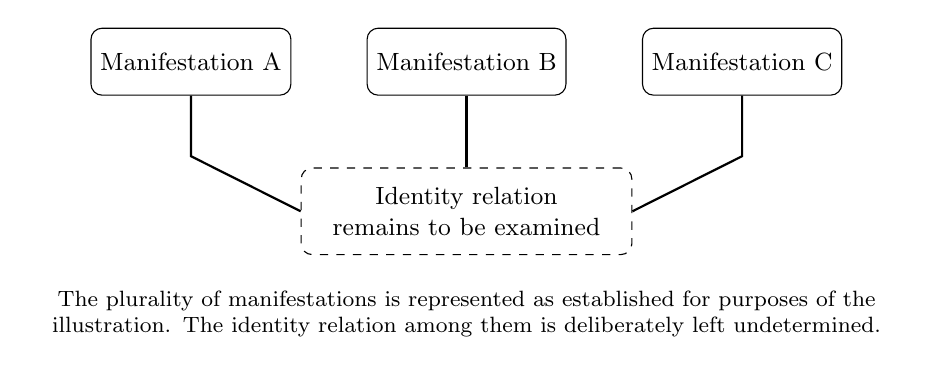
\begin{tikzpicture}[
    manifestation/.style={
        draw,
        rounded corners,
        minimum width=2.1cm,
        minimum height=0.85cm,
        align=center,
        font=\small
    },
    question/.style={
        draw,
        rounded corners,
        dashed,
        minimum width=4.2cm,
        minimum height=1.1cm,
        align=center,
        font=\small
    },
    relation/.style={
        thick,
        -
    }
]

\node[manifestation] (m1) at (-3.5,1.5) {Manifestation A};
\node[manifestation] (m2) at (0,1.5) {Manifestation B};
\node[manifestation] (m3) at (3.5,1.5) {Manifestation C};

\node[question] (identity) at (0,-0.4) {
    Identity relation\\
    remains to be examined
};

\draw[relation] (m1.south) -- (-3.5,0.3) -- (identity.west);
\draw[relation] (m2.south) -- (identity.north);
\draw[relation] (m3.south) -- (3.5,0.3) -- (identity.east);

\node[
    align=center,
    text width=0.9\textwidth,
    font=\footnotesize
] at (0,-1.7) {
    The plurality of manifestations is represented as established
    for purposes of the illustration. The identity relation among
    them is deliberately left undetermined.
};

\end{tikzpicture}

\caption{Plurality of Manifestations and the Unresolved Identity Relation}
\label{fig:manifestation-plurality-and-identity-scope}
\end{figure}

% =============================================================================
% END OF ILLUSTRATION IL01
% =============================================================================

The illustration distinguishes the plurality of
manifestations from the identity question associated
with them. It deliberately leaves the identity
relation unresolved: the diagrammatic grouping of
manifestations is not intended to assert that
they necessarily belong to one identity or to
multiple identities. Its purpose is to make visible
the gap between a manifestational description
and an identity conclusion.

The relation between manifestation and identity
therefore remains an independent ontological problem.
Any conclusion concerning identity must be supported
by grounds that address the identity relation itself,
rather than by the number, similarity, difference,
or grouping of manifestations alone.

% -----------------------------------------------------------------------------
\subsection{The Limit of Numerical Enumeration}

Numerical enumeration cannot provide an exhaustive
account of unity or plurality. Counting requires
a domain of enumeration, a criterion of distinction,
and a specification of what is being counted.
Different criteria may produce different numerical
descriptions of the same broader configuration.
A composition may be counted as one composed
subject while its components are counted as several
elements. A broader configuration may be counted
as one aggregate while several existents remain
distinguishable within it.

Such descriptions are not necessarily contradictory
because they may concern different subjects or
respects. Their compatibility, however, does not
mean that numerical classification is arbitrary.
A count may be precise within its intended domain.
Its limitation concerns the range of conclusions
that may legitimately be drawn from it.

Numerical variation does not by itself determine
the ontological number of identities. The criterion
of enumeration may identify components, material
units, relations, manifestations, or aggregates,
but the identity status of the counted items
requires a separate analysis. A count of several
components is not yet a count of several identities;
a count of one aggregate is not yet a count of
one identity.

The distinction is particularly important when
a numerical description is transferred from one
level of analysis to another. The fact that a
configuration is one under a criterion of
aggregation does not establish that it is one
under a criterion relevant to identity. Likewise,
the fact that several units are distinguished
under a material or relational criterion does
not establish that several identities are involved.

Numerical classification may therefore contribute
to ontological analysis, but it cannot replace it.
The ontological significance of a numerical result
must be established through an account of the
relation between the counted subject, the criterion
of enumeration, and the determination under
investigation.

% -----------------------------------------------------------------------------
\subsection{The Limit of Treating Unity and Plurality as Opposites}

Unity and plurality are often presented as
mutually exclusive alternatives. This opposition
becomes misleading when the relevant subject,
domain, and ontological respect are not specified.
A configuration may be unified in one respect
and plural in another. The unity of an aggregate
may coexist with the plurality of its components;
the unity of a source may coexist with the
plurality of its manifestations; and a broader
configuration involving multiple identities
may exhibit unity under a different determination.

These possibilities do not establish that every
form of unity and plurality can coexist without
qualification. If unity and plurality are attributed
to the same subject, in the same respect, under
the same conditions, their compatibility cannot
simply be assumed. The apparent opposition must
be examined to determine whether the claims
actually concern the same determination or whether
one of them changes its subject, scope, or criterion.

The distinction between respects is therefore
not a device for dissolving every contradiction.
It is a requirement for identifying the content
of each claim. If the subjects or respects differ,
the claims may be compatible. If they are identical,
a further account is required to determine whether
the predicates are genuinely incompatible or
whether the terms have been used in different senses.

Unity and plurality must consequently not be
treated as unrestricted logical opposites. Their
relation depends on what is unified, what is plural,
and the respect in which each determination is
asserted. A conclusion about compatibility or
incompatibility must follow from that analysis,
not from the words alone.

% -----------------------------------------------------------------------------
\subsection{The Limits of Reduction to One Ontological Respect}

Unity and plurality cannot be adequately examined
when all ontological determinations are reduced
to a single respect. Material constitution,
composition, structural organization, relational
determination, manifestation, and identity are
not interchangeable categories. They may be
related within an existent, but the relation
does not make their respective questions identical.

A plurality established in one of these respects
cannot automatically be transferred to another.
Material plurality does not necessarily establish
plurality of identity. Relational plurality does
not necessarily establish multiple existents.
Plurality of determinations does not necessarily
establish plurality of identities. Conversely,
unity in material constitution does not
automatically establish unity of identity, and
structural organization does not independently
prove that the organized subject has one identity.

Every inference across ontological respects
requires an account of the relation that makes
the inference legitimate. It is not enough to
point out that two determinations belong to
the same existent or configuration. Their
co-occurrence does not establish that one
determines the other. A relation of constitution,
dependence, realization, or manifestation may
be relevant, but its ontological significance
must be established rather than assumed.

The following diagram distinguishes several
respects in which unity or plurality may be
examined. It does not arrange them into a
hierarchy, nor does it assert that one respect
grounds or determines another.

% =============================================================================
% Project : THE_PHILOSOPHY_OF_VIABILITY
% Book    : Book I — Ontology of Viability
% Book ID : VS.B01
%
% File    : 4_ASSETS/diagrams/VS.B01.P01.C03.S08.SS12.P003.DG01.limits_of_inference_across_ontological_respects.tex
%
% Asset:
%   Diagram DG01 — Limits of Inference Across Ontological Respects
%
% Purpose :
%   To distinguish several ontological respects in which unity
%   and plurality may be examined, and to show that conclusions
%   established in one respect do not automatically transfer
%   to another.
%
% =============================================================================

\begin{figure}[htbp]
\centering

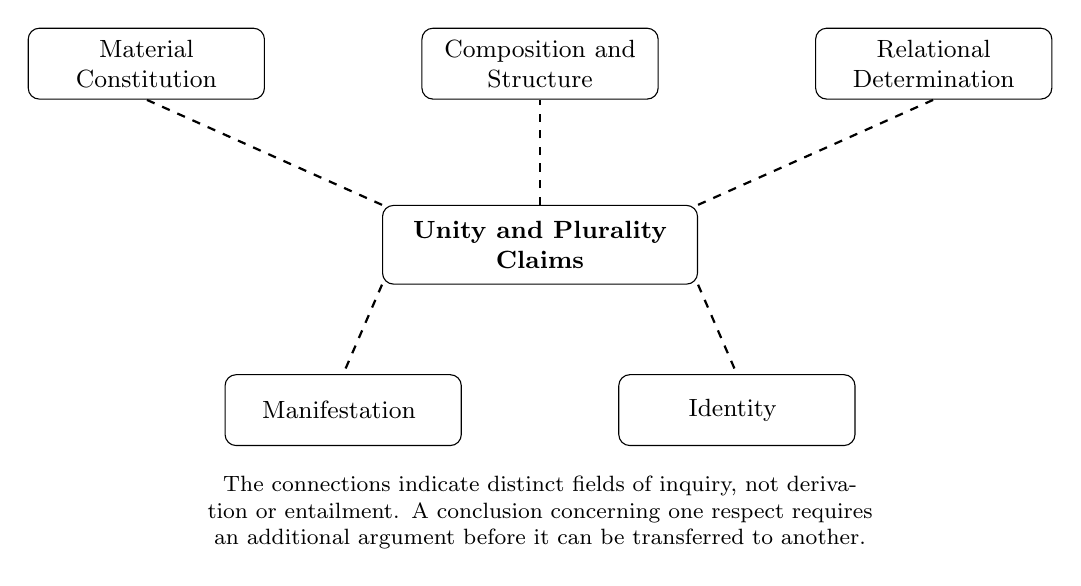
\begin{tikzpicture}[
    respect/.style={
        draw,
        rounded corners,
        align=center,
        minimum width=3.0cm,
        minimum height=0.9cm,
        font=\small
    },
    central/.style={
        draw,
        rounded corners,
        align=center,
        minimum width=4.0cm,
        minimum height=1.0cm,
        font=\small\bfseries
    },
    nonentailment/.style={
        dashed,
        thick,
        -
    }
]

\node[central] (inquiry) at (0,0) {
    Unity and Plurality\\
    Claims
};

\node[respect] (material) at (-5,2.3) {
    Material\\
    Constitution
};

\node[respect] (composition) at (0,2.3) {
    Composition and\\
    Structure
};

\node[respect] (relation) at (5,2.3) {
    Relational\\
    Determination
};

\node[respect] (manifestation) at (-2.5,-2.1) {
    Manifestation
};

\node[respect] (identity) at (2.5,-2.1) {
    Identity
};

\draw[nonentailment] (inquiry.north west) -- (material.south);
\draw[nonentailment] (inquiry.north) -- (composition.south);
\draw[nonentailment] (inquiry.north east) -- (relation.south);
\draw[nonentailment] (inquiry.south west) -- (manifestation.north);
\draw[nonentailment] (inquiry.south east) -- (identity.north);

\node[
    align=center,
    text width=0.92\textwidth,
    font=\footnotesize
] at (0,-3.4) {
    The connections indicate distinct fields of inquiry,
    not derivation or entailment. A conclusion concerning
    one respect requires an additional argument before
    it can be transferred to another.
};

\end{tikzpicture}

\caption{Limits of Inference Across Ontological Respects}
\label{fig:limits-of-inference-across-ontological-respects}
\end{figure}

% =============================================================================
% END OF DIAGRAM DG01
% =============================================================================

The diagram is an analytical map of possible
questions, not a complete inventory of the
ontology and not a causal or derivational model.
Its purpose is to prevent a determination
established in one respect from being transferred
to another without an explicit argument.

The reduction of all these questions to one
respect would conceal rather than resolve the
ontological problems under examination. A
satisfactory account must preserve the distinctions
while examining the relations among them.

% -----------------------------------------------------------------------------
\subsection{Unresolved Questions Concerning Identity and Number}

The restrictions established above leave several
ontological questions open. These questions are
not open merely because the relevant terms have
not yet been defined. They concern relations and
conditions that cannot be settled through unity,
plurality, or numerical classification alone.

Among the unresolved questions are:

\begin{itemize}
    \item Under what ontological conditions can
    an existent be established as involving
    exactly one identity?

    \item Under what conditions, if any, can
    multiple identities be involved in one
    existent or broader configuration?

    \item What grounds distinguish a plurality
    of manifestations from a plurality of identities?

    \item How are the identity boundaries of
    components related to the boundaries of
    a composition or aggregate?

    \item Can unity be established across
    different ontological respects without
    presupposing a single identity?

    \item What ontological relations connect
    a source with multiple manifestations
    without reducing source to manifestation
    or identity to source?

    \item What conditions make a distinction
    among elements relevant to identity rather
    than merely to material, structural,
    relational, or manifestational description?

    \item How should the possibility of identity
    plurality be assessed without presupposing
    that every existent has exactly one identity
    or that every differentiated configuration
    contains several identities?
\end{itemize}

These questions require further ontological
examination of identity, determination,
composition, relation, and manifestation.
They cannot be settled merely by defining
unity as oneness or plurality as multiplicity.
Nor should their openness be mistaken for
evidence that every proposed possibility
is equally established.

The present inquiry establishes restrictions
on what may be inferred. It does not claim
that the unresolved alternatives have already
been demonstrated. Their status must remain
provisional or open until the relevant
ontological grounds have been examined.

% -----------------------------------------------------------------------------
\subsection{Methodological Restrictions}

The analysis of unity and plurality must observe
a set of methodological restrictions. These
restrictions govern the formulation and evaluation
of ontological claims; they are not a substitute
for the substantive arguments required in each
particular case.

First, every claim of unity or plurality must
identify its subject. A statement that something
is one or multiple is incomplete if it does not
make clear what is being counted, unified,
distinguished, or related.

Second, the ontological respect and domain of
the claim must be specified. A conclusion
established concerning material constitution
cannot be transferred automatically to identity,
and a conclusion concerning manifestation
cannot be transferred automatically to source.

Third, numerical descriptions must not be treated
as complete ontological determinations. Counting
may be accurate within a domain while leaving
the identity status of the counted subject
unresolved.

Fourth, plurality of components, relations,
determinations, processes, or manifestations
must not be converted automatically into
plurality of identities. The ontological status
of the distinguished elements requires
independent examination.

Fifth, unity of source, aggregate, composition,
or structure must not be converted automatically
into unity of identity. Each form of unity
concerns a particular subject and respect.

Sixth, the distinction between unity and plurality
must not be used to impose a universal ontological
priority. Neither determination has been shown
to be an unrestricted ground from which all
other determinations can be derived.

Seventh, a distinction among respects must not
be introduced merely to protect a preferred
conclusion from criticism. The relevant respects
and their relations must be independently
specified, and apparent contradictions must
be examined rather than dismissed.

The methodological requirements and the
conclusions they restrict are summarized in
Table~\ref{tab:methodological-limits-of-unity-and-plurality}.

% =============================================================================
% Project : THE_PHILOSOPHY_OF_VIABILITY
% Book    : Book I — Ontology of Viability
% Book ID : VS.B01
%
% File    : 4_ASSETS/tables/VS.B01.P01.C03.S08.SS13.P003.TL01.methodological_limits_of_unity_and_plurality.tex
%
% Asset:
%   Table TL01 — Methodological Limits of Unity and Plurality
%
% Purpose :
%   To summarize the principal restrictions governing claims
%   about unity, plurality, and their implications for identity.
%
% =============================================================================

\begin{table}[htbp]
\centering
\caption{Methodological Limits of Unity and Plurality}
\label{tab:methodological-limits-of-unity-and-plurality}
\footnotesize
\renewcommand{\arraystretch}{1.2}

\begin{tabularx}{\textwidth}{
    @{}
    p{0.24\textwidth}
    X
    p{0.32\textwidth}
    @{}
}
\toprule
\textbf{Analytical Requirement} &
\textbf{Restriction} &
\textbf{Inference Not Licensed by Itself}
\\
\midrule

Specify the subject &
Identify what is unified, plural, counted, or distinguished. &
Unity of one subject establishes unity of another subject.
\\

Specify the respect &
Identify the ontological determination under examination. &
Material, relational, or manifestational plurality establishes identity plurality.
\\

Specify the domain &
Identify the range within which the claim is valid. &
A local numerical result applies to every ontological domain.
\\

Specify the criterion &
Identify what counts as one or multiple. &
Numerical classification determines ontological identity-number.
\\

Preserve conceptual distinctions &
Keep source, aggregate, composition, structure, manifestation, and identity distinct. &
Unity or plurality in one category settles another category.
\\

Establish cross-respect relations &
Provide grounds for transferring a conclusion between respects. &
Co-occurrence of determinations establishes entailment.
\\

Preserve unresolved questions &
Do not convert insufficient evidence into a universal conclusion. &
Failure to prove plurality establishes singular identity, or vice versa.
\\

\bottomrule
\end{tabularx}
\end{table}

% =============================================================================
% END OF TABLE TL01
% =============================================================================

These requirements define conditions for
responsible ontological inference. They do
not constitute a universal definition of
unity, plurality, or identity. Nor do they
settle the final structure of every existent.
Their function is to ensure that an argument
does not claim more than its premises and
ontological grounds establish.

% -----------------------------------------------------------------------------
\subsection{Conclusion: The Scope and Limits of Unity and Plurality}

Unity and plurality are indispensable for
examining the ontological organization of
existents. Their significance, however,
does not make either an unrestricted
explanation of identity, source, composition,
aggregate, structure, or manifestation.

Unity does not establish numerical singularity
or exactly one identity. Plurality does not
establish multiple identities. The unity
of a source or aggregate does not automatically
determine the identity of what is related
to it, and the plurality of components or
manifestations does not automatically
determine the plurality of identities involved.

The analysis has also established that
conclusions must remain within the scope
of the subject and respect for which they
were justified. A determination established
in one ontological respect may be relevant
to another, but relevance does not establish
entailment. The relation must be demonstrated
through an argument appropriate to the
ontological questions involved.

The unresolved questions concerning
identity-number and the relations among
identities must therefore remain open
where the available grounds do not settle
them. This openness is not an endorsement
of every possible answer. It is a refusal
to treat an unsupported inference as an
established ontological result.

The chapter's final section will synthesize
the distinctions developed throughout
the inquiry. It will identify the results
that can be retained, the claims whose
scope has been restricted, and the questions
that remain unresolved, without converting
those results into a premature universal
theory of unity, plurality, or identity.

% =============================================================================
% END OF SECTION 08 OF CHAPTER 03
% =============================================================================

% ------------------------------------------------------------
% SECTION 09
% ------------------------------------------------------------

% =============================================================================
% Section 09 — Synthesis of Unity and Plurality
% Book I — Ontology of Viability
% Chapter 03 — Unity and Plurality
%
% Purpose:
%   To synthesize the ontological distinctions established
%   throughout the chapter and clarify the results that can
%   be retained without imposing a premature resolution
%   of the relation between unity, plurality, and identity.
%
% Conceptual Policy:
%   1. Unity and plurality remain distinct ontological determinations.
%   2. Neither unity nor plurality receives universal priority.
%   3. Unity is not equivalent to singularity.
%   4. Plurality is not equivalent to multiplicity alone.
%   5. Source, aggregate, composition, and identity remain distinct.
%   6. Multiplicity of manifestations does not establish
%      plurality of identities.
%   7. Unity of an aggregate does not establish unity of identity.
%   8. The number of identities remains an independent
%      ontological question.
%
% =============================================================================

\section{Synthesis of Unity and Plurality}
\label{sec:synthesis-of-unity-and-plurality}

% -----------------------------------------------------------------------------
\subsection{The Result of the Inquiry}

The preceding sections have examined unity
and plurality as fundamental but non-equivalent
determinations within the ontology of existents.

The inquiry has not sought to establish
one as the universal foundation of the other.

Rather, it has examined the conditions
under which unity and plurality can be
attributed, the subjects to which such
attributions apply, and the limits of
the inferences that can be drawn from them.

The principal result is that unity and
plurality cannot be adequately understood
through numerical description alone.

Nor can either be reduced to composition,
source, manifestation, or identity.

Their ontological significance depends
on the subject and respect under examination.

The chapter therefore establishes a framework
of distinctions through which claims about
unity and plurality can be evaluated without
prematurely determining the number or
organization of identities.

% -----------------------------------------------------------------------------
\subsection{Unity and Plurality as Distinct Determinations}

Unity and plurality must first be retained
as distinct determinations.

Unity concerns the ontological respect
in which a subject is considered unified.

Plurality concerns the presence of
distinguishable multiple subjects or
elements within a specified domain
and respect.

Their distinction does not imply that
they are universally incompatible.

A subject may exhibit unity in one respect
while involving plurality in another.

Likewise, a plurality of entities may
participate in a configuration that
exhibits unity under a different
ontological determination.

The relation between unity and plurality
must therefore be established through
the identification of their respective
subjects and domains.

Neither concept can be applied without
qualification to every aspect of an existent.

% -----------------------------------------------------------------------------
\subsection{Unity and Singularity}

One of the principal distinctions
established in this chapter concerns
the non-equivalence of unity and
numerical singularity.

Unity is not simply the condition
of being numerically one.

Singularity concerns numerical
determination within a specified
domain of enumeration.

Unity concerns an ontological respect
in which something is unified.

Consequently:

\[
\text{Unity}
\neq
\text{Numerical Singularity}
\]

Numerical oneness does not independently
establish unity of identity.

Likewise, unity does not automatically
establish that exactly one identity
is involved.

This distinction prevents the numerical
classification of an existent from
being treated as a complete account
of its ontological identity.

% -----------------------------------------------------------------------------
\subsection{Unity of Identity and Unity of Source}

The inquiry has also distinguished
unity of identity from unity of source.

A source may be considered one in
a particular respect without this
determining the identity of everything
related to it.

A common source does not automatically
establish one identity among its
manifestations or related entities.

Conversely, plurality among manifestations
does not automatically establish plurality
of sources.

Source relations and identity relations
must therefore remain analytically distinct.

The ontological significance of a source
cannot be exhausted by its relation
to the number of manifestations or
entities associated with it.

% -----------------------------------------------------------------------------
\subsection{Unity of Aggregate and Unity of Identity}

Unity of aggregate must likewise be
distinguished from unity of identity.

An aggregate may constitute a unified
configuration through relations among
its components.

However, the unity of that configuration
does not independently determine whether
one or multiple identities are involved.

The components may retain ontological
distinctions that cannot be eliminated
merely by describing them as parts
of one aggregate.

Similarly, the existence of multiple
components does not automatically
negate every form of unity within
the aggregate.

The following distinction remains
fundamental:

\[
\text{Unity of Aggregate}
\neq
\text{Unity of Identity}
\]

The relation between aggregate and
identity requires an independent
ontological account.

% -----------------------------------------------------------------------------
\subsection{Plurality of Components, Relations, and Manifestations}

The chapter has distinguished plurality
of elements from plurality of identities.

An existent may involve multiple:

\begin{itemize}
    \item Components.
    \item Determinations.
    \item Relations.
    \item Manifestations.
    \item Processes.
    \item Configurations.
\end{itemize}

The presence of these forms of multiplicity
does not automatically establish that
multiple identities are involved.

Multiplicity is therefore not equivalent
to plurality of identities.

The distinction is especially important
because different ontological respects
may contain different forms of plurality
without requiring that they be transferred
to the domain of identity.

The number and organization of identities
must be examined independently of the
mere number of components, relations,
or manifestations.

% -----------------------------------------------------------------------------
\subsection{Plurality of Identities and Composition}

The possibility of multiple identities
must remain distinct from the plurality
of components within a composition.

A composition may contain multiple
components without each component
constituting a distinct identity.

Conversely, the possibility of multiple
identities within a broader configuration
cannot be excluded merely because
that configuration is described
as one composition.

Composition may be relevant to the
determination of identity, but it cannot
serve as its universal or exclusive
foundation.

The relation between identity and
composition must therefore be examined
without assuming that their boundaries
necessarily coincide.

% -----------------------------------------------------------------------------
\subsection{The Independence of Ontological Questions}

The distinctions developed in this
chapter establish that several questions
must not be collapsed into one another.

In particular, the following questions
are analytically distinct:

\begin{enumerate}
    \item Whether a subject is unified
    in a specified ontological respect.

    \item Whether something is numerically
    singular within a particular domain.

    \item Whether a plurality of components
    constitutes one aggregate.

    \item Whether multiple entities share
    a common source.

    \item Whether an existent possesses
    one identity or involves multiple
    identities.

    \item Whether multiple manifestations
    belong to one identity or to distinct
    identities.

    \item Whether a composition and the
    identities involved in it have
    corresponding ontological boundaries.
\end{enumerate}

These questions may be related,
but their relations must be established
rather than assumed.

An answer to one does not automatically
provide an answer to the others.

This analytical independence is necessary
to prevent the reduction of identity
to numerical classification, source,
composition, or manifestation.

% -----------------------------------------------------------------------------
\subsection{A Framework for Examining Unity and Plurality}

The results of the chapter can be
organized through a set of methodological
requirements.

Every claim concerning unity or plurality
must identify:

\begin{itemize}
    \item The subject to which the claim applies.
    \item The ontological respect being examined.
    \item The domain within which the claim is made.
    \item The distinctions required to identify
    the relevant units or elements.
    \item The limits of the inference being drawn.
\end{itemize}

These requirements do not constitute
a universal definition of unity or
plurality.

They establish the minimum conditions
for making such claims without confusing
different ontological determinations.

The framework also prevents a determination
established in one respect from being
transferred to another without justification.

For example, material unity cannot
automatically be converted into unity
of identity, just as relational plurality
cannot automatically be converted into
plurality of identities.

% -----------------------------------------------------------------------------
\subsection{Established Results and Unresolved Questions}

The inquiry supports several conclusions
that can be retained as results of
the present chapter.

First, unity and plurality are not
equivalent to numerical singularity
and numerical multiplicity.

Second, unity and plurality are not
universally mutually exclusive.

Third, unity of source, aggregate,
or composition does not independently
establish unity of identity.

Fourth, plurality of components,
relations, or manifestations does
not independently establish plurality
of identities.

Fifth, identity cannot be reduced
to numerical classification or
compositional organization.

These conclusions establish restrictions
on ontological inference.

They do not, however, settle every
question concerning the number of
identities within an existent.

Several issues remain open:

\begin{itemize}
    \item The ontological conditions
    under which singular identity
    is established.

    \item The conditions under which
    multiple identities may be involved
    in one broader configuration.

    \item The relation between identity
    boundaries and compositional boundaries.

    \item The ontological relation between
    a source and its multiple manifestations.

    \item The conditions under which
    unity may extend across different
    ontological respects.

    \item The possibility and limits
    of identity plurality within an
    existent or a broader configuration.
\end{itemize}

These questions require further analysis
and must not be resolved through
assumptions introduced by the concepts
of unity or plurality themselves.

% -----------------------------------------------------------------------------
\subsection{The Ontological Significance of the Distinctions}

The distinctions established in this
chapter are not merely terminological.

They prevent different ontological
questions from being treated as though
they were interchangeable.

Without these distinctions, numerical
oneness may be mistaken for identity
unity, aggregate unity for singular
identity, or manifestational plurality
for identity plurality.

Such reductions would obscure the
ontological structure of the problems
under examination.

The distinction between unity and
plurality therefore provides a necessary
condition for the further analysis
of identity and manifestation.

It preserves the possibility that
different ontological respects may
exhibit different forms of unity and
plurality without requiring their
reduction to one determination.

This result is methodological and
ontological in significance.

It clarifies what can be established
and what remains to be demonstrated.

% -----------------------------------------------------------------------------
\subsection{Transition to the Further Ontology of Identity}

The present chapter has established
that unity and plurality cannot
independently determine the number
or structure of identities.

The inquiry into identity must therefore
proceed without treating unity as
proof of singular identity or plurality
as proof of multiple identities.

The next stages of the ontology must
examine the conditions through which
identity is constituted, distinguished,
and related to the other determinations
of an existent.

Such an examination must preserve
the distinctions established here
while investigating the ontological
relations that remain unresolved.

The results of this chapter consequently
provide a conceptual restriction
and a methodological foundation
for the further development of
the ontology of viability.

% =============================================================================
% End of Section 09
% =============================================================================

% ------------------------------------------------------------
% CHAPTER CONCLUSION
% ------------------------------------------------------------

\section*{Chapter Conclusion}
\addcontentsline{toc}{section}{Chapter Conclusion}

This chapter has examined unity and plurality as
distinct but interrelated ontological problems within
the ontology of viability.

The analysis has established that assertions of unity
and plurality require specification of their subject
and respect. Without such specification, it is not
possible to determine whether a claim concerns identity,
source, aggregate, composition, determination, relation,
or manifestation.

The chapter has also maintained the distinction between
unity of identity, unity of source, and unity of aggregate.
These forms of unity cannot be assumed to possess the
same ontological meaning or to entail one another
without further argument.

Likewise, plurality of components, relations, determinations,
or manifestations cannot be treated as sufficient evidence
for plurality of identities. The relation between
multiplicity within an existent and the possible
multiplicity of identities remains a question requiring
independent examination.

The distinction between unity and singularity further
prevents the assumption that every assertion of unity
necessarily establishes numerical singularity. Unity
and singularity must therefore remain analytically
distinguishable.

The chapter has not established a universal rule according
to which every existent must possess exactly one identity,
nor has it established that an existent may necessarily
possess multiple identities. These possibilities have
been retained as subjects of ontological inquiry rather
than treated as predetermined conclusions.

Consequently, the analysis provides a framework for
examining the relations between identity, unity, plurality,
source, aggregate, and composition without reducing
any of these concepts to another.

The question of how unity and plurality are ultimately
grounded within the broader architecture of the ontology
of viability remains open for further development.
The distinctions established here provide the basis
for subsequent investigations into the ontological
determinations and manifestations of an existent.

% ============================================================
% END OF CHAPTER 03
% ============================================================



% -----------------------------------------------------------------------------
% CHAPTER 04
% MANIFESTATION
% -----------------------------------------------------------------------------

% ============================================================
% CHAPTER 04
% EXPRESSION
% Book I: Ontology of Viability
% Part I: Identity and Manifestation
% ============================================================

\chapter{Expression}
\label{ch:expression}

% ------------------------------------------------------------
% CHAPTER METADATA
% ------------------------------------------------------------

\newcommand{\ChapterFourTitle}{Expression}
\newcommand{\ChapterFourID}{VS.B01.P01.C04}

% ------------------------------------------------------------
% OPENING QUOTATION
% ------------------------------------------------------------

% ------------------------------------------------------------
% CHAPTER INTRODUCTION
% ------------------------------------------------------------

\section*{Introduction}
\addcontentsline{toc}{section}{Introduction}

Expression constitutes a distinct ontological problem
concerning the relation between an existent and that
through which its determinations, configurations, or
other ontological aspects may become articulated.

The inquiry into expression must not begin by identifying
it with identity, determination, invariance, source,
multiplicity, or manifestation. Nor should expression
be treated in advance as a property, process, relation,
or independently existing entity.

The ontological status of expression, its possible
necessity, and its relations to other fundamental
determinations remain matters of investigation.

The central concern of this chapter is therefore not
merely to describe the ways in which an existent may
be expressed, but to examine whether expression has
a distinct ontological status and how that status
may be related to the identity and constitution
of an existent.

This inquiry proceeds through a series of distinctions
and relational analyses. It begins with the ontological
problem of expression, examines its relation to identity
and determination, and then considers its connections
with invariance, source, multiplicity, and manifestation.

The chapter concludes by examining the limits of
expression and synthesizing the distinctions established
throughout the inquiry.

% ------------------------------------------------------------
% SECTION 01
% ------------------------------------------------------------

% =============================================================================
% Section 01 — The Ontological Problem of Expression
% Book I — Ontology of Viability
% Chapter 04 — Expression
%
% Purpose:
%   To formulate the ontological problem of expression
%   and establish the conceptual questions required
%   for its examination throughout the chapter.
%
% Conceptual Policy:
%   1. Expression is examined as an ontological problem,
%      independently of any knowing subject.
%   2. Expression is not identified with identity,
%      determination, invariance, source, or manifestation.
%   3. The necessity and ontological status of expression
%      are not assumed in advance.
%   4. Expression is not presumed to be a process,
%      property, relation, or independent existent
%      before these possibilities are examined.
%   5. Multiplicity of expressions does not establish
%      plurality of identities.
%   6. No universal relation between expression
%      and manifestation is presupposed.
%   7. The subject and ontological respect of every
%      claim concerning expression must be specified.
%
% =============================================================================

\section{The Ontological Problem of Expression}
\label{sec:ontological-problem-of-expression}

% -----------------------------------------------------------------------------
\subsection{The Question of Expression}

The problem of expression concerns the ontological
status of the ways in which an existent may be
determined, articulated, or presented beyond
the mere attribution of existence and identity.

An existent is not necessarily exhausted by
the statement that it exists or by the recognition
that it possesses an identity.

Its ontological constitution may involve
determinations, relations, configurations,
and forms through which it acquires particular
modes of articulation.

The question is whether, and in what sense,
such articulation requires a distinct ontological
concept of expression.

The term expression is frequently used to describe
the outward articulation of something that
is already determined.

However, this usage may conceal several different
questions.

Does expression designate a determination
of an existent?

Does it designate a relation between an existent
and something through which it is articulated?

Does it designate a process through which
a configuration becomes manifest?

Or does it identify an ontological condition
that cannot be reduced to determination,
relation, or manifestation?

These questions cannot be answered merely
by adopting the ordinary meaning of expression.

They require an examination of the ontological
conditions under which expression can be
meaningfully attributed.

The present section therefore formulates
the problem without assuming that expression
is necessarily an intrinsic property,
an external process, or an independent
ontological entity.

% -----------------------------------------------------------------------------
\subsection{Expression as an Ontological Rather Than Epistemic Problem}

Expression is frequently discussed in relation
to communication, representation, interpretation,
signification, and the transmission of content.

Such discussions often presuppose a subject
who expresses something, another subject
who receives it, or a medium through which
a meaning becomes accessible.

These relations belong to important domains
of inquiry, but they cannot provide the
foundational basis for the present investigation.

The ontology of expression must be examined
independently of whether an existent is
perceived, understood, interpreted, or recognized.

An existent does not acquire its ontological
determinations merely because a subject
becomes aware of them.

Likewise, the absence of a knowing subject
does not by itself establish the absence
of every form of expression.

The relevant question concerns the ontological
relation between an existent and the ways
in which its determinations may be articulated.

Expression must therefore not be defined
exclusively through the act of expressing
a thought, communicating a meaning,
or representing an object.

Such activities may constitute particular
forms of expression within other domains,
but they do not exhaust the ontological
problem examined here.

% -----------------------------------------------------------------------------
\subsection{The Difference Between Existence and Expression}

The recognition of an existent does not
automatically settle the question of expression.

Existence concerns the ontological actuality
of an existent.

Expression concerns a further question
about the possible articulation of that
existent and its determinations.

These questions are related, but they
must not be treated as interchangeable.

The existence of an existent does not,
by itself, establish the specific manner
in which it may be expressed.

Conversely, the recognition of an expression
does not independently establish the
existence or identity of whatever is
taken to be expressed.

An expression cannot simply replace
the existent to which it is related.

Nor can the ontological status of an existent
be reduced to the particular expressions
through which it may be articulated.

The distinction may be stated as follows:

\[
\text{Existence}
\neq
\text{Expression}
\]

This distinction does not establish
that expression is external to existence.

It establishes only that the two concepts
address different ontological questions.

Whether expression is intrinsic to an existent,
dependent upon it, relationally constituted,
or otherwise related to existence remains
a question for further examination.

% -----------------------------------------------------------------------------
\subsection{The Difference Between Identity and Expression}

The relation between identity and expression
constitutes one of the central problems
of this chapter.

Identity concerns the ontological identity
of an existent.

Expression concerns the possible articulation
of an existent or of its determinations.

The distinction must be maintained even
if expression is eventually shown to be
intrinsically related to identity.

An existent cannot be assumed to be identical
with every expression attributed to it.

Nor can the totality of its expressions
be assumed to provide an exhaustive
account of its identity.

A particular expression may articulate
some determinations while leaving other
ontological aspects outside its scope.

Likewise, differences among expressions
do not automatically establish differences
among identities.

The following distinction is therefore
necessary:

\[
\text{Identity}
\neq
\text{Expression}
\]

This does not imply that identity and
expression are unrelated.

It prevents their relation from being
defined through an unexamined equivalence.

The conditions under which expression
belongs to, depends upon, or is related
to identity must be established through
a separate ontological argument.

% -----------------------------------------------------------------------------
\subsection{Expression and Determination}

Expression must also be distinguished
from determination.

Determination concerns the ontological
specification of an existent through
particular determinations.

Expression concerns the question of
how an existent or its determinations
may be articulated.

A determination may be ontologically
attributable to an existent without
thereby being identical with an expression.

Likewise, an expression may involve
or depend upon determinations without
being reducible to their mere presence.

The distinction raises several questions.

Does expression introduce a determination
that was not previously established?

Does it articulate a determination
without altering its ontological status?

Can an existent possess determinations
without those determinations being
expressed in a particular respect?

Can expression itself be understood
as a mode of determination, or does
it designate a distinct relation?

These questions remain open at this stage.

The concept of expression must not
be used as an alternative name for
determination before the relation
between them has been examined.

% -----------------------------------------------------------------------------
\subsection{Expression and the Problem of Invariance}

The relation between expression and
invariance introduces another important
ontological difficulty.

An existent may undergo transformations
while certain determinations remain
invariant under specified conditions.

However, the presence of invariance
does not independently establish
the nature or possibility of expression.

Nor does a change in expression necessarily
establish a change in identity.

An expression may vary while some
ontological determinations remain
unchanged.

Conversely, the persistence of an invariant
does not prove that the same expression
is maintained across different conditions.

The distinction can be stated as:

\[
\text{Expression}
\neq
\text{Invariance}
\]

The relation between them requires
an account of the transformations,
domains, and respects involved.

It must not be assumed that expression
is merely the preservation or disclosure
of invariant features.

The chapter will therefore examine
whether invariance constrains expression,
whether expression may vary under
invariant conditions, and whether
their relation is more complex than
a direct correspondence.

% -----------------------------------------------------------------------------
\subsection{Expression and Source}

The problem of expression also raises
the question of its relation to source.

An expression may be described as
an expression of something.

Such a description introduces a relation
between what is expressed and the
expression attributed to it.

However, the identification of a source
does not automatically explain the
ontological status of expression.

A common source may be related to
multiple expressions without this
establishing that those expressions
are identical.

Likewise, differences among expressions
do not automatically establish multiple
sources.

The relation between source and expression
must therefore be distinguished from
the relation between source and identity.

It is also necessary to avoid assuming
that a source must always exist as
a separate entity standing behind
its expressions.

Whether source is ontologically prior,
co-constitutive, relationally determined,
or related in another manner remains
open to examination.

The problem of source must consequently
be addressed without reducing expression
to a simple transmission from an origin
to an external recipient.

% -----------------------------------------------------------------------------
\subsection{Expression and Multiplicity}

The possibility of multiple expressions
introduces a further distinction between
expression and identity.

An existent may be associated with
multiple expressions, but their multiplicity
does not automatically establish
a plurality of identities.

Likewise, the recognition of one expression
does not establish that only one identity
is involved.

Several different questions must remain
distinct:

\begin{itemize}

    \item Whether an existent can have
    multiple expressions.

    \item Whether multiple expressions
    belong to one and the same existent.

    \item Whether different expressions
    articulate different determinations.

    \item Whether expressions are related
    to one another through a common source.

    \item Whether multiple expressions
    involve one identity or multiple
    identities.

    \item Whether the plurality of expressions
    is simultaneous, successive, or
    dependent upon different ontological
    conditions.

\end{itemize}

These questions cannot be settled
through the mere observation that
multiple expressions are present.

The distinction between multiplicity
of expressions and plurality of identities
must remain explicit throughout
the chapter.

% -----------------------------------------------------------------------------
\subsection{The Problem of Expression and Manifestation}

Expression and manifestation are closely
related concepts, but their relation
cannot be assumed to be one of equivalence.

Manifestation concerns the ontological
presentation or occurrence of something
in a particular mode or domain.

Expression concerns the possible
articulation of an existent or its
determinations.

It remains to be established whether
expression constitutes a condition
of manifestation, whether manifestation
is one possible form of expression,
or whether the two concepts designate
distinct but related ontological relations.

A manifestation may be discussed
without assuming that every aspect
of the manifested existent has been
expressed.

Likewise, an expression cannot
automatically be identified with
the manifestation through which
it may become present.

The distinction is particularly important
because an existent may possess
determinations that are not exhausted
by any particular manifestation.

The relation between expression
and manifestation must therefore
be examined without presupposing
that one is merely another name
for the other.

% -----------------------------------------------------------------------------
\subsection{The Question of the Ontological Necessity of Expression}

A central question concerns whether
expression is necessary to the ontological
constitution of an existent.

There are several possible positions.

Expression may be considered an intrinsic
ontological determination of every existent.

It may be considered a condition that
arises only under particular relations
or circumstances.

It may be understood as a mode through
which already established determinations
are articulated.

Alternatively, expression may designate
a distinct ontological relation whose
necessity depends upon the structure
of the existent under examination.

These possibilities cannot be treated
as equivalent.

Nor can the necessity of expression
be established merely by observing
that existents may have manifestations,
relations, or determinations.

A demonstration is required that distinguishes
the ontological necessity of expression
from its possible occurrence.

The present chapter therefore does
not assume that every existent must
express itself in every respect,
or that the absence of an identified
expression implies the absence of
existence or identity.

The question of necessity remains
one of the principal tasks of the inquiry.

% -----------------------------------------------------------------------------
\subsection{The Risk of Reducing Expression to a Single Ontological Function}

The concept of expression may be reduced
to several different functions.

It may be treated as:

\begin{itemize}

    \item The external presentation of
    an already constituted existent.

    \item The articulation of determinations.

    \item The transmission of something
    from a source.

    \item The preservation of invariant
    features across transformations.

    \item The multiplication of manifestations.

    \item The production of a new existent
    or configuration.

    \item The relation between an existent
    and a domain in which it becomes
    articulated.

\end{itemize}

Each of these descriptions may identify
a possible aspect of expression.

However, none can be accepted as
an exhaustive definition without
further argument.

Reducing expression to one of these
functions may conceal other ontological
relations and impose a structure that
has not yet been established.

The inquiry must therefore determine
whether these functions belong to
one concept, several distinct concepts,
or different aspects of a more complex
ontological relation.

% -----------------------------------------------------------------------------
\subsection{The Subject and Respect of Expression}

Every ontological claim concerning
expression must identify its subject
and respect.

The subject may be an existent,
an identity, a determination, a source,
a configuration, or a manifestation.

The respect may concern material,
structural, relational, or other
ontological determinations.

These subjects and respects must not
be treated as interchangeable.

An expression attributed to an existent
does not necessarily express its identity
in its entirety.

An expression of a determination does
not necessarily constitute an expression
of the whole existent.

Likewise, an expression occurring
in one ontological respect cannot
automatically be transferred to
another respect.

The specification of subject and respect
is therefore necessary to avoid
unrestricted claims about expression.

Without this specification, it remains
unclear what is expressed, in what sense
it is expressed, and what ontological
consequences may legitimately be inferred.

% -----------------------------------------------------------------------------
\subsection{Methodological Requirements for the Inquiry}

The examination of expression requires
several methodological restrictions.

First, expression must be examined
independently of epistemic acts and
the presence of a knowing subject.

Second, it must remain distinct from
identity, determination, invariance,
source, multiplicity, and manifestation
until their relations have been established.

Third, the necessity of expression
must be demonstrated rather than assumed.

Fourth, the plurality of expressions
must not be converted automatically
into plurality of identities.

Fifth, expression must not be reduced
to external presentation, transmission,
or the disclosure of an invariant.

Sixth, claims concerning expression
must specify their subject, domain,
and ontological respect.

Finally, the absence of a particular
expression must not be treated as
proof of the absence of existence,
identity, or determination.

These requirements establish the
conceptual conditions for the analysis
developed in the subsequent sections.

They do not constitute a final theory
of expression.

% -----------------------------------------------------------------------------
\subsection{Scope of the Present Section}

The present section has formulated
the ontological problem of expression
and identified the principal distinctions
necessary for its examination.

It has not established a final definition
of expression.

It has not demonstrated that expression
is universally necessary.

It has not determined whether expression
is intrinsic, relational, processual,
or dependent upon particular conditions.

Nor has it settled the relation between
expression and manifestation.

These questions are deliberately retained
for the subsequent sections.

The next section examines the relation
between identity and expression.

It will investigate whether expression
belongs intrinsically to identity,
whether identity can be distinguished
from its expressions, and what ontological
consequences follow from their relation.

% =============================================================================
% End of Section 01
% =============================================================================

% ------------------------------------------------------------
% SECTION 02
% ------------------------------------------------------------

% =============================================================================
% Section 02 — Identity and Expression
% Book I — Ontology of Viability
% Chapter 04 — Expression
%
% Purpose:
%   To examine the ontological relation between identity and
%   expression without reducing either concept to the other.
%
% Conceptual Policy:
%   1. Identity and expression are distinct ontological questions.
%   2. Expression must not be treated as the totality or definition
%      of identity.
%   3. Identity must not be reduced to the capacity for expression.
%   4. Neither an exclusively internal nor an exclusively external
%      relation between identity and expression is presupposed.
%   5. Multiplicity of expressions does not establish plurality
%      of identities.
%   6. The ontological necessity and status of expression remain
%      open to examination.
% =============================================================================

\section{Identity and Expression}
\label{sec:identity-and-expression}

\subsection{The Problem of Relating Identity to Expression}

The relation between identity and expression constitutes
one of the central problems in the ontological analysis
of expression.

An existent may be considered in terms of its identity
and also in terms of the ways in which aspects of its
being are expressed. These two considerations are
related, but their relation cannot be assumed to be
one of equivalence.

Identity concerns the ontological identity of an existent.
Expression concerns a distinct question regarding the
ontological status and articulation of what belongs to,
proceeds from, or is otherwise related to an existent.

The distinction does not imply that identity and expression
are unrelated. It establishes only that their relation
requires examination rather than conceptual identification.

The central question is therefore not whether identity
and expression can be mentioned together, but how
expression is related to identity without becoming
a substitute for it.

Several possibilities must be considered. Expression
may be related to identity as one of its determinations,
as an articulation of aspects belonging to it, as a
mode through which certain features become manifest,
or through some other ontological relation not yet
adequately specified.

None of these possibilities should be adopted as a
complete account before its ontological implications
have been examined.

\subsection{Identity Is Not the Totality of Its Expressions}

A first distinction concerns the possibility of reducing
identity to the totality of expressions associated with
an existent.

An existent may exhibit multiple expressions across
different relations, conditions, domains, or circumstances.
These expressions may vary in form, scope, intensity,
configuration, or persistence.

It does not follow that the identity of the existent
is constituted by the sum of these expressions.

Such a reduction would require demonstrating that
every ontological aspect relevant to identity is
exhaustively represented by expression, and that no
distinction remains between the identity of the existent
and the expressions associated with it.

That requirement has not been established.

The totality of expressions may provide a description
of certain aspects of an existent, but descriptive
completeness within a domain does not necessarily
amount to ontological completeness.

Even if every currently identifiable expression were
enumerated, the enumeration itself would not establish
that identity is nothing beyond that collection.

The distinction between an existent and the expressions
associated with it must therefore remain analytically
available.

Identity cannot be defined simply as the aggregate
of expressions without an independent argument
establishing the sufficiency of such a reduction.

\subsection{Expression Is Not the Definition of Identity}

The reduction of identity to expression may also occur
when expression is treated as the defining criterion
of what an existent is.

According to such a reduction, an existent would be
understood through what it expresses, and its identity
would be determined by the content or configuration
of those expressions.

This approach risks confusing the characterization
of an existent with its ontological identity.

A characterization may identify features, relations,
or configurations through which an existent can be
described or distinguished. Yet the availability of
such descriptions does not establish that the existent's
identity is exhausted by them.

An expression may be relevant to the characterization
of an existent without constituting the complete
ontological basis of its identity.

Likewise, a change in an expression does not by itself
establish a change in identity. Such a conclusion would
require an additional account of the relation between
the particular expression that changes and the identity
of the existent to which it is related.

The ontological significance of an expression must
therefore be assessed according to its specific relation
to the existent, rather than inferred from the mere
presence or alteration of expression.

\subsection{Identity Is Not Identical to the Capacity for Expression}

A further possibility is to define identity through
the capacity of an existent to express itself.

This formulation differs from reducing identity to
actual expressions. Instead of identifying identity
with what is expressed, it identifies identity with
the capacity or potentiality for expression.

However, this proposal also requires examination.

The capacity to express may be an important feature
of certain existents. Yet its presence does not by itself
establish the identity of the existent, nor does its
absence, where applicable, automatically establish
the absence of identity.

To define identity through expressive capacity would
require showing that this capacity is ontologically
necessary for identity and that it is sufficiently
distinctive to account for identity rather than merely
for one of its possible characteristics.

Such a demonstration cannot be assumed.

Moreover, the concept of capacity introduces further
questions concerning the ontological status of
potentiality, its relation to actuality, and the
conditions under which a capacity may or may not
be realized.

These questions cannot be resolved merely by
identifying identity with the capacity for expression.

Identity and expressive capacity must therefore
remain distinguishable until their relation has
been established.

\subsection{Expression as an Aspect, Determination, or Relation of Identity}

Although identity cannot be reduced to expression,
the possibility that expression is ontologically
related to identity must not be excluded.

Expression may belong to the analysis of an existent
in a manner that is neither identical with identity
nor entirely external to it.

One possibility is that expression concerns certain
aspects or determinations of an existent. In this case,
expression would be related to what the existent is
without being equivalent to the identity of the existent.

Another possibility is that expression articulates
a relation between an existent and some aspect of
its ontological constitution. This would require
clarifying the terms of that relation and determining
whether expression is itself a relation, a feature
of a relation, or something ontologically different.

A further possibility is that expression is associated
with the ways in which an existent is manifested.
However, such a possibility must preserve the distinction
between expression and manifestation. Their relation
cannot be settled by treating them as interchangeable
terms.

These possibilities indicate that the relation between
identity and expression may be more complex than
either simple equivalence or complete separation.

The task is to determine the nature and limits of
that relation without assigning expression an
ontological function that has not yet been justified.

\subsection{The Internal and External Interpretations of Expression}

The relation between identity and expression may
also be approached through the distinction between
internal and external interpretations.

An internal interpretation may regard expression
as belonging to the ontological constitution of
the existent itself. Under this interpretation,
expression would not merely be an external description
or an incidental consequence of the existent.

An external interpretation, by contrast, may regard
expression as something that occurs in relation
to the existent without necessarily belonging to
its constitutive identity.

Neither interpretation should be accepted without
qualification.

If expression is treated as entirely internal,
the distinction between identity and expression
may be obscured. Expression may become an assumed
component of identity without a sufficient account
of why it must be so.

If expression is treated as entirely external,
its possible ontological significance may be
prematurely excluded. The relation between an
existent and its expressions may involve more than
an accidental or merely descriptive association.

The internal and external interpretations therefore
identify different possible structures of relation,
but neither establishes the complete ontological
status of expression.

It remains necessary to examine particular cases
and determine the relevant subject, respect, and
ontological conditions of each proposed relation.

\subsection{The Difference Between Identity and Expressive Configuration}

An existent may be associated with an organized
configuration of expressions.

Such a configuration may include multiple expressions
that are related to one another through a particular
order, structure, or pattern. It may also exhibit
regularities, variations, and relations of dependence.

The existence of an organized expressive configuration
does not establish that the configuration itself
constitutes the identity of the existent.

A configuration of expressions and the identity
of an existent are different objects of ontological
analysis.

The former concerns the organization of expressions;
the latter concerns the identity of the existent.

Their relation may be constitutive, dependent,
correlative, or of another kind. But the existence
of organization alone does not determine which
relation obtains.

Nor does the unity of an expressive configuration
necessarily establish the unity of identity.
Conversely, the plurality of expressions within
a configuration does not establish a plurality
of identities.

These distinctions are especially important where
an existent is associated with several domains,
relations, or forms of expression.

The organization of expressions must not be confused
with the ontological unity or plurality of the
existent's identity.

\subsection{Expression, Change, and the Question of Identity Preservation}

The relation between identity and expression becomes
particularly significant when expressions change.

An existent may undergo alterations in the form,
configuration, or conditions of its expressions.
Such alterations may occur while other aspects
of the existent remain unchanged.

However, the persistence of some expressions does
not by itself establish the persistence of identity,
just as the alteration or disappearance of particular
expressions does not by itself establish the loss
of identity.

The question of identity preservation must be
examined independently of the mere continuity
or discontinuity of expressions.

This distinction is consistent with the broader
distinction between identity and invariance.

An invariant may remain preserved across a specified
transformation, but the preservation of that invariant
does not automatically establish the identity of
the existent. Likewise, an expression may change
without this change necessarily implying that
identity has changed.

The relevant question is whether a particular
expression has an ontologically established relation
to identity such that its alteration bears upon
the identity of the existent.

Without such an account, the transition from
expressive change to identity change remains
unjustified.

\subsection{Multiplicity of Expressions and the Unity or Plurality of Identity}

The relation between identity and expression also
raises the question of multiplicity.

An existent may be associated with multiple expressions.
These may differ according to domain, relation,
configuration, or conditions of occurrence.

Such multiplicity does not, by itself, determine
whether the existent possesses one identity or
multiple identities.

A plurality of expressions may belong to one existent
without establishing a plurality of identities.
Equally, the existence of a unified expressive
configuration cannot by itself establish that
the existent possesses only one identity.

The question of identity plurality requires an
independent ontological analysis.

The number of expressions, the number of expressive
configurations, the number of domains in which
expression occurs, and the number of identities
must not be treated as interchangeable quantities.

Each concerns a different aspect of the ontological
problem.

Accordingly, neither unity nor plurality of identity
can be inferred solely from the multiplicity or
organization of expressions.

\subsection{The Non-Exhaustive Relation Between Identity and Expression}

The distinctions established above suggest that
the relation between identity and expression should
be treated as non-exhaustive.

Expression may be relevant to the ontological analysis
of identity, but its relevance does not establish
that it exhausts identity.

Identity may provide an ontological reference for
the examination of expression, but this does not
establish that expression is merely a secondary
description without independent significance.

The relation must therefore remain open to more
precise determination.

At this stage, it is possible to establish several
restrictions:

\begin{enumerate}
    \item Identity must not be reduced to the totality
    of expressions associated with an existent.

    \item Identity must not be defined solely through
    the capacity for expression.

    \item Expression must not be assumed to constitute
    identity merely because it is associated with
    an existent.

    \item The alteration of an expression must not
    automatically be interpreted as a transformation
    of identity.

    \item The multiplicity of expressions must not
    be treated as proof of a plurality of identities.

    \item The unity of an expressive configuration
    must not be treated as proof of the singularity
    or numerical unity of identity.
\end{enumerate}

These restrictions do not provide a complete theory
of the relation. They establish the conceptual
conditions under which that relation may be
investigated without collapsing distinct ontological
questions into one another.

\subsection{Open Questions Concerning Identity and Expression}

Several questions remain unresolved.

Is expression necessarily related to the identity
of every existent, or is it applicable only under
specific ontological conditions?

If expression is related to identity, does it belong
to the constitution of the existent, arise from
some of its determinations, articulate certain
relations, or occupy another ontological position?

Can an existent possess an identity independently
of any particular expression, and, if so, what
would such independence mean ontologically?

Can expression be altered, suspended, or absent
without affecting identity?

Under what conditions, if any, can an alteration
in expression have consequences for identity?

Does the relation between identity and expression
remain the same across different domains and
forms of existence?

These questions cannot be answered through
terminological definition alone. They require
further analysis of determination, invariance,
source, multiplicity, and manifestation.

The present section therefore establishes the
distinction between identity and expression
without claiming to have completed the account
of their ontological relation.

\subsection{Transition to Expression and Determination}

The distinction between identity and expression
raises a further question concerning determination.

If expression is neither identical with identity
nor reducible to its totality, it becomes necessary
to examine whether expression is related to the
determinations of an existent and, if so, how
that relation should be understood.

Determination concerns what specifies or delimits
an existent in a particular ontological respect.
Expression may be related to such determinations,
but it cannot be assumed that every determination
is an expression or that every expression is
itself a determination.

The next section examines this relation while
preserving the distinctions established here.

% =============================================================================
% End of Section 02
% =============================================================================

% ------------------------------------------------------------
% SECTION 03
% ------------------------------------------------------------

% =============================================================================
% Section 03 — Expression and Determination
% Book I — Ontology of Viability
% Chapter 04 — Expression
%
% Purpose:
%   To examine the ontological relation between expression
%   and determination without reducing either concept to the other.
%
% Conceptual Policy:
%   1. Expression and determination are analytically distinct.
%   2. Not every determination is necessarily an expression.
%   3. Not every expression is necessarily a determination.
%   4. Expression must not be reduced to the articulation or
%      disclosure of determinations.
%   5. Determination must not be defined through expression alone.
%   6. Their relation must be examined according to subject
%      and respect.
% =============================================================================

\section{Expression and Determination}
\label{sec:expression-and-determination}

\subsection{The Ontological Problem of Expression and Determination}

The relation between expression and determination constitutes
a further problem in the ontological analysis of expression.

An existent may possess determinations through which
its ontological constitution is specified, delimited,
or differentiated. It may also be associated with
expressions that raise a distinct question concerning
how aspects of its being are articulated.

The presence of both determination and expression
does not establish that they are identical or that
one can be reduced to the other.

Determination concerns the ontological specification
of an existent in a particular respect. Expression
concerns the ontological status of an articulation
or expression associated with an existent. The precise
meaning of expression remains under examination,
but its distinction from determination must be
preserved throughout that inquiry.

The central problem is therefore to establish whether
expression is a determination, depends upon determinations,
articulates determinations, or stands in another
ontological relation to them.

These possibilities must not be treated as equivalent.
Each implies a different account of the constitution
of an existent and of the role that expression may
occupy within it.

\subsection{Determination as Ontological Specification}

Determination concerns the specification of an existent
in a particular ontological respect.

An existent is not adequately described merely by
asserting that it exists. Its determinations may
establish particular ways in which it is constituted,
distinguished, related, or delimited.

Determination therefore belongs to the analysis
of what specifies an existent, rather than necessarily
to the analysis of how that existent is expressed.

A determination may be ontologically significant
even when no corresponding expression has been
identified. The absence of an identified expression
does not establish the absence of determination.

Likewise, the identification of a determination
does not automatically establish that the determination
has been expressed.

This distinction prevents determination from being
made dependent upon the occurrence, recognition,
or description of expression.

Determination must therefore be examined according
to its own ontological conditions, even where it
is subsequently found to be related to expression.

\subsection{Expression Cannot Be Presumed to Be a Determination}

One possible interpretation treats expression as
a determination of an existent.

According to this interpretation, to express would
be one of the ways in which an existent is determined.
Expression would consequently occupy a position
within the ontological constitution of the existent
alongside other determinations.

This possibility cannot be excluded in advance.
However, it cannot be accepted merely because
expression is associated with an existent.

The fact that something belongs to, proceeds from,
or is related to an existent does not establish
that it is a determination of that existent.

To classify expression as a determination would
require an account of what expression specifies,
delimits, or establishes in the existent and
why this function should be understood as
determination rather than through another
ontological category.

Furthermore, if expression is treated as a determination,
it becomes necessary to distinguish between the
determination that makes expression possible and
the expression itself.

Otherwise, the concept risks becoming circular:
expression would be explained as a determination
while the relevant determination would itself
be identified only through expression.

The classification of expression as a determination
must therefore remain a possible interpretation,
not an established premise.

\subsection{Not Every Determination Is Necessarily Expressed}

The relation between determination and expression
must also be examined from the opposite direction.

Even if certain expressions are found to articulate
or correspond to determinations, it does not follow
that every determination must be expressed.

A determination may belong to the ontological
constitution of an existent without being associated
with an identifiable expression.

The possibility of unexpressed determination
must therefore remain conceptually available.

To deny this possibility would require establishing
that expression is a necessary condition for the
existence or ontological efficacy of every
determination.

Such a requirement has not yet been demonstrated.

Moreover, the distinction between the existence
of a determination and its expression prevents
the ontological status of the former from being
made dependent upon the latter.

A determination does not cease to be ontologically
relevant merely because no corresponding expression
has been established.

This does not imply that determination is always
independent of expression. It means only that
their dependence cannot be presumed to be universal.

\subsection{Not Every Expression Is Necessarily a Determination}

The converse restriction is equally important.

Even where an expression is established, it does
not follow that the expression itself constitutes
a determination of the existent.

An expression may be related to a determination
without being identical to it. It may articulate
a determination, arise under conditions established
by determinations, or stand in another relation
that does not make it a determination in its own right.

The distinction is necessary because the classification
of every expression as a determination would eliminate
the possibility that expression has a distinct
ontological status.

Such a reduction would also make the analysis
of expression dependent upon the conceptual
framework of determination, leaving no independent
question concerning what expression itself is.

An expression may therefore be examined as an
expression even when its relation to determination
has not been established.

Whether a particular expression is itself a
determination must be decided according to
the ontological role it occupies, not according
to the mere fact that it is associated with
an existent.

\subsection{Expression as Articulation of Determination}

A further possibility is that expression articulates
or gives form to certain determinations of an existent.

Under this interpretation, determination and
expression remain distinct, while expression
is understood through a relation to what has
already been ontologically specified.

This possibility may explain why an existent can
possess determinations that are not exhausted
by the particular expressions associated with it.

However, the term articulation must itself be
used carefully.

If articulation means that expression makes
a determination available to a recipient,
it introduces an epistemic or communicative
framework that does not belong to the present
ontological inquiry.

If articulation is intended in a strictly
ontological sense, its meaning must be specified
without presupposing a knower, interpreter,
observer, or receiving consciousness.

The ontological relation may concern the way
in which a determination is configured, related,
or expressed within the being of an existent.
Yet the exact nature of this relation remains
to be established.

Accordingly, expression as articulation of
determination is a possible account, but it
cannot serve as a complete definition of
expression without further argument.

\subsection{Expression and the Configuration of Determinations}

Determinations may occur in organized configurations.

An existent may possess several determinations
whose relations establish a particular structure
or configuration. These determinations may be
mutually dependent, hierarchically ordered,
or related through other forms of organization.

Expression may be associated with such configurations.
It may concern a particular determination, a relation
among determinations, or a configuration considered
as a whole.

These possibilities must remain distinct.

An expression associated with one determination
does not necessarily express the entire configuration.
Likewise, an expression associated with a configuration
does not establish that every determination within
that configuration is independently expressed.

The relation between expression and configuration
therefore requires specification of its subject
and respect.

A further distinction must be preserved between
the organization of determinations and the organization
of expressions. Even where these organizations
correspond, they are not necessarily identical.

The structure of an existent cannot be inferred
exhaustively from the structure of its expressions
without demonstrating the ontological adequacy
of that inference.

\subsection{Determination, Expression, and Ontological Dependence}

The relation between expression and determination
may involve different forms of ontological dependence.

Expression may depend upon certain determinations
because those determinations establish conditions
under which a particular expression can occur.

Alternatively, a determination may depend upon
expression if expression is shown to contribute
to the constitution or specification of the existent
in a particular respect.

A reciprocal relation may also be possible, although
such reciprocity cannot be assumed merely because
the two concepts are related.

The existence of a relation does not establish
its direction, symmetry, or degree of dependence.

It is therefore necessary to distinguish among:

\begin{enumerate}
    \item The dependence of expression upon determination.
    \item The dependence of determination upon expression.
    \item Reciprocal dependence between expression
    and determination.
    \item A relation between them that involves
    neither constitutive dependence nor equivalence.
\end{enumerate}

These alternatives have different ontological
implications.

In particular, the possibility that expression
depends upon determination does not establish
that expression is reducible to determination.
Dependence and identity are different relations.

Similarly, the possibility that expression contributes
to a determination does not establish that determination
is nothing beyond expression.

The precise form of dependence must therefore
be established independently in each relevant case.

\subsection{Expression and the Distinction Between Determination and Identity}

The relation between expression and determination
must also preserve the distinction between both
concepts and identity.

Determination does not exhaust identity, and
expression does not exhaust determination.

An existent may possess determinations through
which aspects of its constitution are specified.
It may also possess expressions related to some
of those determinations.

However, neither the totality of determinations
nor the totality of expressions can be assumed
to constitute the identity of the existent.

This restriction is particularly important because
the identification of an organized set of determinations
may create the appearance of a complete account
of an existent.

Yet a complete description of determinations
within a specified analytical domain is not
necessarily equivalent to an exhaustive account
of identity.

The same applies to expressions.

The ontological analysis must therefore preserve
three distinct questions:

\begin{enumerate}
    \item What determines or specifies the existent?
    \item What is expressed, and what is the ontological
    status of that expression?
    \item What constitutes the identity of the existent?
\end{enumerate}

The answers may be related, but they cannot be
treated as interchangeable.

\subsection{Expression, Determination, and Change}

The distinction between expression and determination
becomes particularly important when an existent
undergoes change.

An existent may undergo a change in one or more
of its determinations. It may also undergo a change
in its expressions without a corresponding change
in the determinations to which those expressions
are related.

Conversely, a determination may change while
a particular expression remains unchanged,
or while no corresponding expressive alteration
has been established.

These possibilities indicate that expressive change
and determinate change cannot be treated as
necessarily equivalent.

A change in expression may be associated with
a change in determination, but the association
does not establish identity between the two changes.

Likewise, the preservation of an expression does
not necessarily establish the preservation of
the determination associated with it.

The analysis must identify what has changed,
the respect in which the change occurred,
and the ontological relation between the relevant
expression and determination.

Without these distinctions, the concept of expression
would become an unreliable substitute for the
analysis of ontological change.

\subsection{The Limits of Inferring Determination from Expression}

An expression may provide grounds for considering
a possible determination, but the existence of
an expression does not automatically establish
the complete determination of the existent.

Such an inference would require an account of
the relation between the expression and the
determination attributed to the existent.

In particular, it would be necessary to establish
whether the expression is constitutive of the
determination, dependent upon it, or merely
associated with it.

The same restriction applies when several expressions
are considered together.

The accumulation of expressions does not necessarily
produce an exhaustive account of determinations.
Nor does an extensive configuration of expressions
establish that every relevant determination has
been accounted for.

The distinction between ontological determination
and the description of expression must therefore
be maintained.

This restriction does not deny that expressions
may be ontologically significant. It prevents
their significance from being extended beyond
what their established relations justify.

\subsection{Subject and Respect in the Relation Between Expression and Determination}

Every claim concerning the relation between
expression and determination must specify
its subject and respect.

A statement that an existent expresses a determination
is incomplete unless it clarifies which existent
is under consideration, which determination
is involved, and in what respect the expression
is related to it.

The same expression may be associated with
different determinations under different conditions.
Likewise, a single determination may be related
to different expressions across distinct domains.

Consequently, the relation cannot be generalized
without identifying the ontological scope within
which it is asserted.

The specification of subject and respect is
particularly important where multiple determinations
and expressions are involved.

Without it, distinct relations may be conflated,
and a local correspondence may be incorrectly
treated as a universal ontological principle.

The analysis of expression and determination
must therefore remain sensitive to the scope
and conditions of each proposed relation.

\subsection{Open Questions Concerning Expression and Determination}

The analysis of this section establishes a number
of distinctions, but it does not settle the complete
ontological relation between expression and determination.

Several questions remain open:

\begin{enumerate}
    \item Is expression itself a determination,
    or does it occupy a distinct ontological category?

    \item Can expression occur without being
    constitutively related to a determination?

    \item Can a determination exist without any
    corresponding expression?

    \item Under what conditions does expression
    articulate, depend upon, or contribute to
    determination?

    \item Can the relation between expression
    and determination be reciprocal?

    \item Do different domains of existence involve
    different relations between expression
    and determination?

    \item What distinguishes an ontological relation
    between expression and determination from
    a merely descriptive correspondence?
\end{enumerate}

These questions require further examination.
They cannot be resolved by assuming that expression
is simply the external appearance of determination
or that determination is merely what expression
makes available.

\subsection{Transition to Expression and Invariance}

The distinction between expression and determination
raises a further problem concerning invariance.

If an existent is associated with determinations
and expressions that may undergo change, it becomes
necessary to examine whether any aspects of expression
remain invariant across specified transformations.

However, the invariance of an expression must not
be confused with the invariance of a determination,
and neither should be treated as equivalent to
the identity of the existent.

The next section examines the relation between
expression and invariance while preserving the
distinctions among identity, determination,
expression, and persistence.

% =============================================================================
% End of Section 03
% =============================================================================

% ------------------------------------------------------------
% SECTION 04
% ------------------------------------------------------------

% =============================================================================
% Section 04 — Expression and Invariance
% Book I — Ontology of Viability
% Chapter 04 — Expression
%
% Purpose:
%   To examine the relation between expression and invariance
%   without reducing expressive continuity to invariant
%   preservation or identifying either with identity.
%
% Conceptual Policy:
%   1. Expression and invariance are distinct ontological problems.
%   2. An invariant expression does not establish identity.
%   3. An alteration in expression does not necessarily establish
%      a transformation of identity.
%   4. Expressive invariance must be specified relative to a
%      transformation, domain, and respect.
%   5. Formal invariance must not automatically be treated
%      as ontological invariance.
%   6. The relation between expression and invariance remains
%      subject to ontological investigation.
% =============================================================================

\section{Expression and Invariance}
\label{sec:expression-and-invariance}

\subsection{The Ontological Problem of Expression and Invariance}

The relation between expression and invariance introduces
a further dimension into the ontological analysis of
expression.

An existent may be associated with expressions that
remain preserved across certain transformations.
It may also be associated with expressions that
undergo alteration, disappear, emerge, or assume
different configurations under changing conditions.

These possibilities raise the question of whether
expression can possess invariance and, if so,
what the preservation of an expression establishes
about the existent to which it is related.

The problem cannot be resolved by identifying
expression with invariance. Expression concerns
a distinct ontological question, whereas invariance
concerns the preservation of a specified feature,
relation, or structure under a specified transformation.

Their relation must therefore be examined without
collapsing the distinction between what is expressed
and what remains invariant.

The central question is not merely whether an
expression persists, but what kind of persistence
is involved, under which transformation it occurs,
and what ontological significance can legitimately
be attributed to it.

\subsection{The Distinction Between Expression and Invariance}

Expression and invariance refer to different
analytical dimensions.

Expression concerns the ontological status and
articulation of something associated with an existent.
Invariance concerns the preservation of a specified
aspect under a transformation.

An expression may be invariant with respect to
a particular transformation. However, this does
not make expression itself equivalent to invariance.

Likewise, an invariant may exist without being
appropriately characterized as an expression.

The distinction is necessary because the same
expression may be invariant under one transformation
and variable under another. Its invariance therefore
cannot be asserted without specifying the relevant
conditions.

Similarly, the fact that an invariant is identified
within an expressive configuration does not establish
that the invariant exhausts the ontological status
of the expression.

Expression and invariance must consequently be
treated as distinct concepts whose possible relations
require independent specification.

\subsection{The Possibility of Invariant Expression}

An expression may remain preserved across a
specified transformation.

For example, an existent may undergo changes in
its conditions, relations, or configurations while
a particular expression remains unchanged in
a defined respect.

This possibility establishes that expression
may be examined in terms of invariance.

However, the claim that an expression is invariant
requires more than the observation that it appears
unchanged.

At minimum, the analysis must specify:

\begin{enumerate}
    \item The expression whose preservation is being examined.
    \item The existent or ontological subject to which
    that expression is related.
    \item The transformation across which preservation
    is asserted.
    \item The domain within which the transformation
    is considered.
    \item The respect in which the expression remains
    invariant.
\end{enumerate}

Without these specifications, the statement that
an expression is invariant remains indeterminate.

An expression may remain unchanged in one respect
while undergoing alteration in another. Its preservation
may therefore be partial rather than comprehensive.

The existence of invariant expression must be
understood relative to the conditions under which
the invariance is established.

\subsection{Invariant Expression Does Not Establish Identity}

The preservation of an expression does not by itself
establish the identity of the existent associated
with it.

An expression may remain invariant across a
transformation without providing sufficient grounds
for concluding that the same numerical identity
has been preserved.

This restriction follows from the distinction
between identity and invariance.

Identity concerns the ontological identity of
the existent. Invariance concerns the preservation
of a specified aspect under a transformation.

Even where an invariant expression is closely
associated with an existent, the preservation
of that expression establishes only what has
been shown to remain preserved in the relevant
respect.

It does not establish that the expression is
sufficient to account for identity.

To infer identity from invariant expression,
an additional ontological argument would be
required. Such an argument would need to establish
why the particular expression is constitutive
of identity and why its preservation is sufficient
for the preservation of that identity.

Without this demonstration, invariant expression
cannot serve as an independent criterion of identity.

\subsection{The Absence of Invariant Expression Does Not Negate Identity}

The converse restriction is equally important.

The failure to identify an invariant expression
does not establish that an existent lacks identity
or that its identity has ceased to persist.

An existent may undergo extensive expressive
alteration. Its expressions may change in form,
configuration, or domain, and previously identifiable
expressions may disappear.

Nevertheless, the absence of a preserved expression
does not by itself establish the absence of identity.

Such a conclusion would require demonstrating
that the particular expression, or the preservation
of expression in general, is ontologically necessary
for the identity of the existent.

That necessity cannot be assumed.

The distinction prevents the analysis of identity
from becoming dependent upon the successful
identification of invariant expressions.

It also prevents the absence of a known invariant
from being confused with the ontological absence
of invariance itself.

The failure to identify an invariant and the
establishment that no relevant invariant exists
are different claims.

Neither claim, by itself, settles the question
of identity.

\subsection{Expression and the Transformation of Determinations}

Expressions may be related to determinations
that undergo transformation.

An existent may undergo changes in its determinations
while certain expressions remain preserved.
Alternatively, an expression may change while
the determination to which it is related remains
preserved in a particular respect.

These possibilities indicate that the transformation
of expression and the transformation of determination
must be examined independently.

A preserved expression does not necessarily establish
the preservation of every determination associated
with it.

Likewise, a changed expression does not necessarily
establish that the corresponding determination
has changed.

The relation between expressive transformation
and determinate transformation must therefore
be established in each relevant case.

It is also possible that a transformation affects
both expression and determination, although the
presence of simultaneous change does not establish
that the two changes are identical or governed
by the same conditions.

The ontological analysis must distinguish what
changes, what remains preserved, and how the
relevant transformations are related.

\subsection{The Relativity of Expressive Invariance}

No claim of expressive invariance is complete
without specifying the transformation relative
to which preservation is asserted.

An expression may remain invariant under one
transformation while changing under another.

It may also remain invariant within one domain
while undergoing alteration across another.

Consequently, expressive invariance must not
be treated as an absolute property merely because
preservation has been established under a limited
set of conditions.

The claim must be indexed to the relevant
transformation, domain, and respect.

This relativity does not imply that invariance
is arbitrary or merely subjective. It means that
the ontological conditions of preservation must
be specified rather than left implicit.

A claim of invariance that omits its transformation
or domain risks extending a limited result into
an unsupported universal statement.

The same methodological requirement applies
to the analysis of expression.

\subsection{Formal and Ontological Invariance of Expression}

The invariance of an expression may be established
within a formal system.

A formal representation may preserve a particular
structure, relation, value, or configuration
under a specified operation.

Such preservation may be mathematically rigorous
and formally demonstrable.

However, formal invariance does not automatically
establish ontological invariance.

A formal system may represent an expression or
some aspect of it, but the preservation of a
formal representation does not by itself establish
that the corresponding ontological feature remains
preserved in the existent.

The transition from formal preservation to
ontological preservation requires an account
of the relation between the formal structure
and the ontological subject under consideration.

This distinction is particularly important where
expressions are represented through symbolic,
mathematical, or structural systems.

The formal preservation of a representation
must not be confused with the ontological
preservation of what that representation concerns.

Formal invariance may provide a basis for
ontological investigation, but it cannot replace
that investigation.

\subsection{Expression, Invariance, and Continuity}

Expression may exhibit continuity across a
sequence of transformations without possessing
an invariant form in every respect.

Continuity and invariance are not equivalent.

An expression may undergo gradual alteration
while maintaining some form of continuity.
Conversely, an expression may remain unchanged
across a specified transformation without this
preservation establishing a broader continuity
of the existent.

The analysis must therefore distinguish between:

\begin{enumerate}
    \item The preservation of an expression.
    \item The continuity of an expressive configuration.
    \item The persistence of an expression across time.
    \item The invariance of a specified feature under
    a transformation.
    \item The continuity or persistence of the existent
    associated with the expression.
\end{enumerate}

These questions may be related, but they concern
different ontological conditions.

The preservation of an expression under a
transformation does not automatically establish
its persistence across all temporal conditions.
Likewise, temporal continuity does not necessarily
establish invariance under every relevant
transformation.

The relation between expression and continuity
must therefore be investigated without reducing
either concept to invariance.

\subsection{The Multiplicity of Invariants Within Expression}

An expressive configuration may contain several
features that remain invariant under different
transformations.

Some features may be preserved across a broad
range of transformations, while others may remain
preserved only under restricted conditions.

The existence of multiple invariants within an
expressive configuration does not establish
that the configuration itself is wholly invariant.

Nor does the plurality of invariants establish
a plurality of expressions or identities.

The number of invariants, the number of expressions,
and the number of identities are distinct matters.

Furthermore, invariants within a configuration
may be related to one another through structural
or relational conditions. Their preservation
may be independent, mutually dependent, or
conditioned by the same transformation.

These relations require separate analysis.

The presence of several invariant features must
not be interpreted as a complete ontological
account of the expression in which they occur.

\subsection{The Transformation of Expression Without Identity Change}

An existent may undergo a transformation in
its expressions without this transformation
necessarily implying a change in identity.

An expression may be replaced by another,
altered in configuration, or associated with
different conditions of occurrence.

Such transformations may be ontologically
significant while remaining insufficient to
establish a transformation of identity.

The conclusion that identity has changed requires
an independent account of the relation between
the transformed expression and the identity
of the existent.

The absence of such an account makes the inference
from expressive transformation to identity
transformation unjustified.

This does not mean that expressive transformation
can never accompany or contribute to a change
in identity.

It means that the relation must be established
rather than assumed.

A transformation of expression and a transformation
of identity are distinct claims, even where they
may occur together.

\subsection{The Limits of Invariance as an Explanation of Expression}

Invariance may explain certain aspects of the
preservation of expression, but it cannot provide
a complete explanation of expression itself.

To define expression through invariance would
exclude expressions that change, emerge, disappear,
or remain variable under particular transformations.

It would also obscure the distinction between
what is expressed and the conditions under which
some aspect of that expression is preserved.

An expression may be ontologically significant
without possessing an invariant feature that
has been established.

Conversely, an invariant structure may be present
without thereby constituting an expression.

Invariance therefore addresses a particular
question concerning preservation, not the entire
ontological problem of expression.

Its explanatory role must remain limited to
the aspects of expression for which a relevant
relation has been demonstrated.

\subsection{Subject and Respect in Expressive Invariance}

Every claim concerning expressive invariance
must identify its subject and respect.

It must be clear which expression is being examined,
which existent is associated with it, and under
which transformation its preservation is asserted.

The relevant respect must also be specified.

An expression may remain invariant in structural
organization while changing in material realization.
It may remain invariant in one relation while
undergoing alteration in another.

These possibilities demonstrate why the unqualified
statement that an expression is invariant may
conceal several distinct claims.

The analysis must distinguish the invariant aspect
from the aspects that remain variable.

It must also avoid extending the preservation
of one feature to the entire expression or
to the identity of the existent.

The specification of subject and respect is
therefore a necessary condition for a precise
ontological account of expressive invariance.

\subsection{Open Questions Concerning Expression and Invariance}

The distinctions established in this section
leave several questions unresolved:

\begin{enumerate}
    \item Can expression possess invariance as
    an ontological feature, or is invariance
    applicable only to particular aspects of
    an expression?

    \item Under what conditions can an expression
    remain invariant while the determinations
    associated with it change?

    \item Can an expression undergo transformation
    without losing its relation to the existent
    with which it is associated?

    \item Is there any ontologically necessary
    relation between expressive invariance
    and the preservation of identity?

    \item Can an expression remain invariant
    across different domains, or is its invariance
    necessarily domain-relative?

    \item What conditions distinguish formal
    invariance of an expression from its
    ontological invariance?

    \item Can an expressive configuration remain
    continuous despite the alteration of all
    its previously identified invariant features?
\end{enumerate}

These questions require further analysis of
the ontological status of expression and its
relations to other aspects of an existent.

\subsection{Transition to Expression and Source}

The analysis of expression and invariance establishes
that the preservation of an expression cannot
be treated as equivalent to the preservation
of identity.

It also demonstrates that expression may be
examined across transformations without being
reduced to the invariants that remain preserved.

A further question concerns the relation between
expression and source.

If an expression is associated with an existent
or emerges under particular ontological conditions,
it becomes necessary to examine whether the concept
of source explains that relation, and whether
the existence of a source establishes anything
definitive about the nature of expression.

The next section examines this problem without
presupposing that every expression must be
understood through a simple origin-to-result
relation.

% =============================================================================
% End of Section 04
% =============================================================================

% ------------------------------------------------------------
% SECTION 05
% ------------------------------------------------------------

% =============================================================================
% Section 05 — Expression and Source
% Book I — Ontology of Viability
% Chapter 04 — Expression
%
% Purpose:
%   To examine the ontological relation between expression
%   and source without reducing expression to origin,
%   derivation, transmission, or causal production.
%
% Conceptual Policy:
%   1. Source and expression are distinct ontological concepts.
%   2. The existence of a source does not by itself explain
%      the ontological status of expression.
%   3. Expression must not be reduced to a linear process
%      of transmission from origin to recipient.
%   4. The relation between source and expression must not
%      be presumed to be exclusively causal or temporal.
%   5. The multiplicity of expressions does not establish
%      the multiplicity of sources or identities.
%   6. The ontological status of source and its relation
%      to expression remain subject to investigation.
% =============================================================================

\section{Expression and Source}
\label{sec:expression-and-source}

\subsection{The Ontological Problem of Expression and Source}

The relation between expression and source constitutes
a further problem in determining the ontological status
of expression.

An expression may be associated with an existent
from which it originates, upon which it depends,
or to which it is otherwise ontologically related.
Such an existent may be considered a source in a
particular respect.

However, the identification of a source does not
by itself explain what expression is.

The source and the expression associated with it
belong to distinct analytical questions. The source
concerns the ontological ground, origin, or condition
of something, whereas expression concerns the
ontological status and articulation of what is
expressed.

These descriptions indicate possible dimensions
of the relation, but they do not establish that
source must always be understood as origin, that
expression must always be understood as an outcome,
or that their relation necessarily involves a
transfer from one existent to another.

The central problem is therefore to determine
whether expression originates from a source,
depends upon it, belongs to it, articulates some
aspect of it, or stands in another ontological
relation that cannot be adequately described
through these categories alone.

The relation must be examined without assuming
that the concept of source provides a complete
explanation of expression.

\subsection{The Distinction Between Source and Expression}

Source and expression must remain conceptually
distinguishable.

A source cannot be identified with an expression
merely because an expression is attributed to it.
Likewise, an expression cannot be identified
with its source merely because it originates
from or depends upon that source.

The distinction concerns the difference between
what occupies the position of source and what
occupies the position of expression.

A source may be considered in relation to several
expressions, while an expression may be related
to a source in a particular ontological respect.

These relations do not establish equivalence
between their terms.

Even where an expression is inseparable from
a particular source under specified conditions,
inseparability does not necessarily imply identity.

The ontological relation between source and
expression must therefore be distinguished
from the identity of source and expression.

This distinction also prevents the source from
being treated as merely the hidden or unexpressed
version of the expression, and prevents expression
from being treated as nothing more than a visible
or external form of its source.

Both reductions require assumptions that have
not yet been justified.

\subsection{Source as Origin and the Limits of Origin-Based Explanation}

One possible interpretation understands source
as the origin from which an expression proceeds.

Under this interpretation, the source occupies
an ontological position prior to the expression,
and the expression is understood through its
relation to that origin.

Such an account may be relevant where an identifiable
origin can be established.

However, origin-based explanation cannot be
presumed to apply universally.

The concept of origin may imply a temporal,
causal, structural, or ontological priority.
These forms of priority are not interchangeable.

A source may be ontologically prior to an expression
without being temporally earlier than it.
Likewise, temporal precedence does not establish
ontological priority.

A causal relation, where present, also does not
necessarily establish that the cause is the
complete ontological source of everything
associated with its effect.

The relation between source and expression
must therefore specify what kind of priority
is being asserted.

Furthermore, an explanation of the origin of
an expression does not necessarily explain
its ontological nature.

Knowing from where an expression originates
does not establish what expression is, what
status it possesses, or how it relates to
the identity of the source.

Origin may explain one aspect of the relation
without exhausting the problem.

\subsection{Expression as Derivation from Source}

A related possibility is to understand expression
as something derived from a source.

Derivation may indicate that an expression
depends upon a source or follows from its
ontological constitution.

However, the term derivation can refer to
different relations.

It may indicate causal production, structural
dependence, ontological consequence, formal
determination, or another relation of dependence.

These relations must not be treated as equivalent.

If expression is derived from a source, it remains
necessary to establish whether the derivation
is necessary or contingent, whether it preserves
particular determinations of the source, and
whether the expression possesses any ontological
conditions not reducible to the source.

The fact that something is derived from another
does not establish that it is identical to that
from which it is derived.

Nor does derivation necessarily imply that
the derived expression is ontologically inferior,
less real, or merely secondary.

Such conclusions would require independent
arguments concerning the ontological status
of the source and the expression.

Derivation may therefore describe a possible
relation between source and expression, but
it cannot serve as a complete definition of
expression.

\subsection{Expression and the Possibility of Ontological Dependence}

The relation between expression and source
may involve ontological dependence.

An expression may depend upon a source for
its existence, constitution, occurrence, or
particular configuration.

However, these forms of dependence must be
distinguished.

An expression may depend upon a source for
its origin without remaining dependent upon
it in every subsequent respect.

It may also depend upon a source for its
ontological constitution while possessing
determinations that are not adequately
described as mere repetitions of the source.

Alternatively, the expression may remain
continuously dependent upon its source under
conditions that must be specified.

The presence of dependence does not establish
its scope or direction.

At least four possibilities must therefore
be distinguished:

\begin{enumerate}
    \item Dependence of expression upon source
    for its existence.

    \item Dependence of expression upon source
    for its particular determinations or configuration.

    \item Dependence of expression upon source
    for its continued existence or persistence.

    \item A relation between source and expression
    that does not amount to constitutive or
    existential dependence.
\end{enumerate}

These possibilities may overlap, but none
can be inferred solely from the identification
of a source.

The ontological dependence of expression
must be established according to the specific
relation under consideration.

\subsection{The Source Does Not Exhaust the Expression}

Even if an expression is established as
originating from or depending upon a source,
it does not follow that the expression is
fully explained by the source alone.

The expression may possess a particular
configuration, determination, or relational
position that requires independent analysis.

Its ontological status cannot be inferred
exhaustively from the ontological status
of its source.

This restriction does not deny the significance
of the source. It prevents the source from
being used as a substitute for examining
the expression itself.

A complete account would need to distinguish
between what is attributable to the source,
what belongs to the relation between source
and expression, and what may be specific
to the expression.

Without these distinctions, the explanation
risks collapsing the expression into a mere
repetition or derivative description of its source.

The source may be necessary for explaining
the existence or constitution of an expression
without being sufficient to explain every
aspect of that expression.

\subsection{The Possibility of Multiple Expressions from a Source}

A source may be associated with multiple
expressions.

These expressions may differ in configuration,
determination, domain, relation, or conditions
of occurrence.

The multiplicity of expressions raises questions
concerning the relation between their source
and their respective ontological conditions.

It does not, however, establish that the source
itself is multiple, that the source possesses
multiple identities, or that each expression
constitutes an independent identity.

A plurality of expressions may be related
to one source without requiring a plurality
of sources.

Conversely, the unity of a source does not
establish that all expressions associated
with it form one undifferentiated expression.

The relations among expressions must be
examined independently of the numerical
or ontological unity of their source.

The analysis must therefore distinguish:

\begin{enumerate}
    \item The number of sources.
    \item The number of expressions.
    \item The number of expressive configurations.
    \item The number of identities associated
    with the relevant existents.
\end{enumerate}

These quantities concern different ontological
questions and cannot be inferred from one another
without further argument.

\subsection{The Source-Expression Relation Is Not Necessarily Linear}

A common interpretation of expression assumes
a linear relation in which a source produces
an expression that is subsequently directed
toward a recipient or destination.

Such a structure may be applicable in particular
cases, but it must not be adopted as a universal
ontological model.

The linear model presupposes distinguishable
positions: an origin, a process of transmission,
an expressed result, and a recipient.

Yet the existence of these positions and the
relations among them require independent
ontological justification.

Expression may occur without an identifiable
recipient. A relation between source and expression
may also be constitutive or structural rather
than transmissive.

Furthermore, the source and the expression
may be related without an intervening process
that can adequately be described as transmission.

The absence of a recipient does not necessarily
negate the existence of expression, just as
the presence of a recipient does not establish
that expression is reducible to communication
or reception.

The source-expression relation must therefore
remain open to forms of ontological organization
that are not adequately captured by a linear
origin-to-recipient sequence.

\subsection{Source, Expression, and Ontological Priority}

The relation between source and expression
may involve questions of ontological priority.

If a source is necessary for the existence
of an expression, it may possess a form of
priority relative to that expression.

However, the nature of this priority must
be specified.

Ontological priority is not necessarily temporal
priority, causal priority, structural priority,
or explanatory priority.

A source may be ontologically prior without
preceding its expression in time.

Likewise, an expression may possess a distinct
ontological status without being independent
of its source in every respect.

The existence of priority does not establish
that the source and expression belong to
different degrees of reality, nor does it
establish that the expression is merely
an inferior derivative.

Such conclusions would require a broader
account of ontological dependence and the
status of the relevant existents.

The analysis must therefore distinguish
the priority of source from the ontological
status of expression.

\subsection{Expression and the Distinction Between Source and Aggregate}

The concept of source must also be distinguished
from the concept of aggregate.

An aggregate may consist of multiple components
or elements organized or associated in a
particular manner. A source, by contrast,
concerns a particular ontological relation
of origin, dependence, or grounding.

The existence of an aggregate does not establish
that it constitutes a source.

Likewise, a source must not be presumed to
be an aggregate merely because multiple
determinations, components, or relations
are associated with it.

This distinction is important when several
expressions are attributed to a source.

The plurality of expressions does not establish
that the source is an aggregate of those expressions.
Nor does the unity of a source establish that
its expressions are reducible to components
of a single aggregate.

The ontological relation between source and
expression must therefore be distinguished
from the compositional relation between
an aggregate and its constituents.

Source, aggregate, expression, and composition
must remain separate analytical categories.

\subsection{Source and Expression Across Different Ontological Domains}

The relation between source and expression
may vary across different ontological domains.

An expression associated with a source in one
domain may not exhibit the same form of dependence
as an expression associated with a source
in another domain.

The conditions under which expression originates,
depends upon, or relates to a source may differ
according to the ontological structure involved.

It would therefore be unjustified to assume
that one model of source-expression relation
applies uniformly to every domain of existence.

Any such generalization would require establishing
that the relevant ontological conditions are
sufficiently equivalent across those domains.

The present analysis does not presume such
equivalence.

The relation must instead be examined according
to its specific subject, domain, and respect.

\subsection{The Limits of Explaining Expression Through Source}

Source may provide an important dimension
of explanation, but it cannot be assumed
to resolve the entire ontological problem
of expression.

Several limitations must be recognized.

First, identifying a source does not establish
the ontological category to which expression belongs.

Second, establishing derivation does not establish
that expression is identical with its source
or exhausted by its origin.

Third, establishing dependence does not determine
the precise scope or direction of that dependence.

Fourth, the unity or plurality of expressions
does not determine the unity or plurality
of sources or identities.

Fifth, an origin-based account does not necessarily
explain the configuration, determinations,
or ontological conditions of expression.

The concept of source must therefore remain
one dimension of the analysis rather than
a universal explanatory principle.

A complete account of expression requires
examining its relations to other ontological
categories without reducing it to any one
of them.

\subsection{Subject and Respect in the Source-Expression Relation}

Every claim concerning source and expression
must identify the relevant subject and respect.

It must be clear which existent is being
considered as the source, which entity or
ontological aspect is being considered as
the expression, and what kind of relation
is being asserted between them.

The same existent may function as a source
in one respect without necessarily occupying
that position in every other respect.

Likewise, an expression may depend upon
a source in one respect while possessing
a distinct configuration or relational status
in another.

The relation must not be generalized beyond
the conditions under which it has been established.

This requirement is especially important
where several sources, expressions, or
ontological domains are involved.

Without specifying subject and respect,
the distinction between source, expression,
and their possible relations becomes unstable.

\subsection{Open Questions Concerning Expression and Source}

The analysis of this section establishes
the distinction between source and expression
while leaving their complete ontological
relation unresolved.

Several questions remain open:

\begin{enumerate}
    \item Is a source ontologically necessary
    for every expression?

    \item Can expression exist without an
    identifiable origin?

    \item Does every source necessarily give
    rise to expression?

    \item Is the relation between source and
    expression necessarily one of dependence?

    \item Can an expression possess ontological
    conditions that are not reducible to its source?

    \item Can a source be related to multiple
    expressions without being an aggregate
    of those expressions?

    \item Can expression occur without a recipient
    or destination?

    \item Are there forms of source-expression
    relation that cannot be adequately described
    through causation, derivation, or transmission?

    \item Does the relation between source and
    expression vary across ontological domains?
\end{enumerate}

These questions require further investigation
and cannot be resolved by assuming a universal
model of origin and derivation.

\subsection{Transition to Expression and Multiplicity}

The analysis of source and expression raises
a further question concerning multiplicity.

A source may be associated with several expressions,
and an existent may participate in multiple
expressive relations.

However, the multiplicity of expressions does
not establish the plurality of sources, identities,
or existents.

It becomes necessary, therefore, to examine
the ontological significance of expressive
multiplicity and to distinguish it from the
plurality of components, relations, manifestations,
and identities.

The next section investigates these distinctions
without presupposing that the multiplicity
of expression necessarily corresponds to
a multiplicity of identity.

% =============================================================================
% End of Section 05
% =============================================================================

% ------------------------------------------------------------
% SECTION 06
% ------------------------------------------------------------

% =============================================================================
% Section 06 — Expression and Multiplicity
% Book I — Ontology of Viability
% Chapter 04 — Expression
%
% Purpose:
%   To examine the ontological significance of multiplicity
%   in expression while distinguishing expressive plurality
%   from plurality of components, relations, manifestations,
%   sources, and identities.
%
% Conceptual Policy:
%   1. Expression and multiplicity are distinct concepts.
%   2. Multiple expressions do not necessarily establish
%      multiple identities.
%   3. The unity of expressions does not necessarily establish
%      the unity or singularity of identity.
%   4. Multiplicity of expression must not be reduced to
%      compositional plurality.
%   5. The number of expressions must not be inferred from
%      the number of sources, domains, or manifestations.
%   6. Neither unity nor plurality of identity is presupposed.
% =============================================================================

\section{Expression and Multiplicity}
\label{sec:expression-and-multiplicity}

\subsection{The Ontological Problem of Expressive Multiplicity}

The relation between expression and multiplicity
raises a fundamental question concerning the
ontological significance of plurality within
the expressive dimension of an existent.

An existent may be associated with several expressions.
These expressions may differ in their configuration,
determinations, relations, domains, or conditions
of occurrence.

The existence of such multiplicity, however,
does not by itself establish what kind of plurality
is involved.

A plurality of expressions may indicate the
multiplicity of expressive forms without establishing
a plurality of sources, components, manifestations,
existents, or identities.

Conversely, the unity of an expressive configuration
does not necessarily establish that the existent
associated with it possesses only one identity.

The central problem is therefore to determine
what multiplicity means when applied to expression
and how expressive plurality relates to other
forms of ontological plurality.

The analysis must preserve the distinction between
the multiplicity of what is expressed, the multiplicity
of expressions, and the multiplicity of the existents
or identities associated with them.

\subsection{The Distinction Between Expression and Multiplicity}

Expression and multiplicity concern different
analytical dimensions.

Expression concerns the ontological status and
articulation of what is expressed. Multiplicity
concerns the presence of more than one distinguishable
item, configuration, relation, or occurrence
within a specified respect.

Multiplicity may therefore apply to expressions
without defining what expression itself is.

The fact that expressions are multiple does not
explain their ontological status, their relation
to their source, or their relation to the existent
with which they are associated.

Likewise, the existence of expression does not
necessarily imply multiplicity.

An existent may be associated with one identifiable
expression, several expressions, or an expressive
configuration whose numerical or structural
character remains undetermined.

Multiplicity must therefore be examined as
a possible feature of expression rather than
as an intrinsic and universal condition of
every expression.

\subsection{The Multiplicity of Expressions}

An existent may be associated with multiple
expressions that are distinguishable from one
another.

Such expressions may differ in form, structure,
configuration, determination, relation, or
ontological domain.

Their differences may be substantial or limited.
They may occur simultaneously or under different
conditions. They may also be related through
dependence, correspondence, coordination,
or other forms of organization.

The presence of multiple expressions does not
establish that they are independent of one another.

Nor does their distinguishability establish
that they are ontologically separate existents.

Several expressions may belong to one expressive
configuration, while multiple configurations
may be related to a common existent or source.

The analysis must therefore distinguish between
the numerical plurality of expressions and
the ontological independence of the expressions
being counted.

A plurality of expressions establishes plurality
within the relevant expressive respect. It does
not automatically establish plurality at every
other ontological level.

\subsection{Multiplicity of Expressions and Plurality of Identities}

The most important restriction concerns the
relation between expressive plurality and
identity plurality.

The existence of multiple expressions does not
by itself establish that the existent associated
with them possesses multiple identities.

An existent may be associated with several
expressions while the question of its identity
remains independent of their numerical plurality.

To infer multiple identities from multiple
expressions would require establishing that
each expression corresponds to a distinct
identity and that the correspondence is
ontologically constitutive rather than merely
descriptive, relational, or configurational.

Such a requirement cannot be satisfied by
counting expressions alone.

Conversely, the presence of one expressive
configuration does not establish that only
one identity is involved.

An apparently unified expressive structure
may contain distinctions that require further
ontological analysis.

The number of expressions and the number
of identities must therefore be treated as
separate questions.

Neither a one-to-one correspondence nor
a many-to-one or one-to-many correspondence
between expressions and identities should
be presumed.

The relation must be established independently
for each relevant ontological subject and respect.

\subsection{Multiplicity of Expressions and Unity of Identity}

A plurality of expressions may be associated
with an existent whose identity is considered
in terms of unity.

However, this possibility must not be interpreted
as proof that the identity of the existent is
necessarily singular or that every expression
belongs to one and only one identity.

Unity of identity and multiplicity of expression
concern different analytical questions.

The unity of identity concerns the ontological
unity of the identity under examination.
Multiplicity of expression concerns the plurality
of expressions associated with a particular
ontological subject or configuration.

Their coexistence is therefore possible without
requiring either concept to be reduced to the other.

The existence of several expressions may be
compatible with a unified identity, but the
precise relation must be established rather
than assumed.

Likewise, the existence of a unified expressive
configuration does not independently settle
the question of identity unity.

\subsection{Multiplicity of Expressions and Singularity}

Multiplicity must also be distinguished from
the question of singularity.

The presence of multiple expressions does
not establish that the existent itself is
non-singular in the relevant ontological respect.

Likewise, the presence of one expression does
not establish the singularity of identity.

Singularity concerns a different ontological
question from the numerical plurality of
expressions.

An existent may be considered singular in
one respect while being associated with
multiple expressions in another.

The coexistence of these conditions does
not constitute a contradiction because
the relevant claims concern different
analytical dimensions.

The distinction between unity and singularity
must therefore be preserved when examining
expressive multiplicity.

Neither the number of expressions nor the
organization of their configuration can
serve as a sufficient criterion for determining
the singularity of identity.

\subsection{Multiplicity of Expression and Multiplicity of Determinations}

An expressive plurality may be associated
with a plurality of determinations.

However, the multiplicity of expressions
and the multiplicity of determinations are
not necessarily equivalent.

Several expressions may be related to one
determination, while one expression may be
associated with several determinations.

It is also possible that some expressions
do not correspond directly to determinations
in the sense previously examined.

The relation between expressive plurality
and determinate plurality must therefore
be specified rather than inferred from
numerical correspondence.

A plurality of determinations may establish
complexity within the ontological constitution
of an existent without establishing a plurality
of expressions.

Conversely, multiple expressions may occur
without establishing an equivalent number
of distinct determinations.

The number of determinations and the number
of expressions must remain analytically
independent unless a specific relation
between them has been demonstrated.

\subsection{Multiplicity of Expression and Composition}

Expressive multiplicity must also be distinguished
from compositional multiplicity.

Composition concerns the constitution of an
existent through components, elements, or
constituents and the relations through which
they form a particular configuration.

Expressive multiplicity concerns the plurality
of expressions associated with an existent
or an expressive configuration.

These two forms of plurality may be related,
but neither can be reduced to the other.

An existent may possess multiple components
without each component constituting a distinct
expression.

Likewise, an existent may be associated with
multiple expressions without those expressions
constituting components of a single aggregate.

To treat expressions as components would require
establishing their compositional role within
the existent.

The mere fact that several expressions are
distinguishable does not establish that they
are constituents of the entity with which
they are associated.

This distinction prevents expressive plurality
from being interpreted automatically as
a plurality of parts or compositional elements.

\subsection{Multiplicity of Expression and Multiplicity of Relations}

An existent may participate in multiple relations,
and these relations may be associated with
different expressions.

However, the plurality of relations does not
necessarily correspond to the plurality of
expressions.

One expression may be related to several
ontological relations, while several expressions
may be associated with one relation or with
different aspects of a relational configuration.

The existence of multiple relations therefore
does not determine the number of expressions.

Likewise, the multiplicity of expressions does
not establish that the existent participates
in an equivalent number of independent relations.

A relation may be constitutive, dependent,
reciprocal, or otherwise structured.
The relation between expression and relational
plurality must be examined according to
the relevant ontological conditions.

The numerical distinction between relations
and expressions must remain available
throughout the analysis.

\subsection{Multiplicity of Expression and Multiplicity of Manifestation}

The multiplicity of expressions must also
be distinguished from the multiplicity of
manifestations.

An existent may be associated with several
manifestations, but this does not establish
that each manifestation constitutes a distinct
expression.

Likewise, several expressions may be associated
with one manifestation or with different
aspects of a manifestation.

The relation between expression and manifestation
requires an independent ontological account.

The two concepts cannot be treated as equivalent
merely because both may involve distinguishable
forms, configurations, or occurrences associated
with an existent.

This distinction is particularly important
because the multiplicity of manifestations
may arise under conditions different from
those governing the multiplicity of expressions.

The number of manifestations cannot therefore
be used as a direct measure of the number
of expressions, nor can the number of expressions
be used as a direct measure of manifestations.

Their correspondence, where present, must
be established within a specified domain
and respect.

\subsection{Multiplicity of Expressions and the Unity of Source}

A source may be associated with multiple
expressions without being identical to their
aggregate.

The unity of a source does not require that
all expressions associated with it be identical,
uniform, or organized as one undifferentiated
configuration.

Likewise, the plurality of expressions does
not establish that the source itself is plural.

The distinction between source and expression
must therefore be preserved when considering
expressive multiplicity.

A single source may be related to several
expressions through different relations or
conditions. Alternatively, several sources
may be associated with expressions that
exhibit similarities or correspondences.

Neither possibility determines the number
of identities involved.

The plurality of expressions, the plurality
of sources, and the plurality of identities
must be examined independently.

In particular, a common source does not
automatically establish a common identity
among all expressions associated with it.

Source unity and identity unity are distinct
ontological questions.

\subsection{The Organization of Expressive Multiplicity}

Multiple expressions may be organized in
different ways.

They may form a coherent configuration,
remain relatively independent, exhibit
hierarchical relations, or be connected
through conditions of dependence or coordination.

The organization of expressions may therefore
introduce structural distinctions within
expressive multiplicity.

However, the existence of organization does
not establish that the expressions constitute
one ontological entity or one identity.

Likewise, the absence of an identified common
organization does not establish that the
expressions are entirely independent.

The organization of expressions must be
examined according to the relations that
actually obtain among them.

Several levels of organization must remain
distinguishable:

\begin{enumerate}
    \item The internal configuration of an
    individual expression.

    \item The relations among multiple expressions.

    \item The organization of expressions
    within a larger expressive configuration.

    \item The relation between that configuration
    and the existent or source with which
    it is associated.
\end{enumerate}

These levels may interact, but their interaction
does not eliminate their analytical distinction.

\subsection{Multiplicity of Expressions Across Ontological Domains}

Expressions may occur across different
ontological domains.

An existent may be associated with expressions
that belong to distinct domains or that relate
to different aspects of its ontological constitution.

The presence of expressions across several
domains does not establish that the existent
possesses a separate identity in each domain.

Nor does it establish that all such expressions
belong to one identity.

Both conclusions would require additional
ontological arguments.

The relevant domains must be distinguished
from the expressions occurring within them.

A plurality of domains is not necessarily
a plurality of expressions, just as a plurality
of expressions across domains is not necessarily
a plurality of identities.

The relation between domains and expressions
must therefore be examined without assuming
a direct numerical correspondence.

\subsection{Multiplicity and the Conditions of Expressive Independence}

The distinction between multiple expressions
and independent expressions requires further
attention.

Two expressions may be distinguishable without
being ontologically independent.

They may depend upon the same source, share
determinations, participate in a common
configuration, or stand in relations that
constrain their occurrence.

Conversely, expressions associated with
different sources may exhibit similar forms
without thereby becoming identical or
ontologically dependent upon one another.

Independence must therefore be distinguished
from numerical plurality.

The existence of multiple expressions establishes
that they are distinguishable within the
relevant analytical respect. It does not
establish the degree or form of their
ontological independence.

An account of expressive multiplicity must
therefore examine whether the expressions
are independent, dependent, interdependent,
or related in some other manner.

These relations must be established rather
than inferred from the mere fact of plurality.

\subsection{The Transformation of Expressive Multiplicity}

The number and configuration of expressions
associated with an existent may change.

An existent may acquire additional expressions,
lose previously associated expressions,
or undergo transformations in the relations
among them.

Such changes may alter the expressive
configuration without necessarily establishing
a change in identity.

Likewise, the preservation of the number
of expressions does not establish the
preservation of their configuration or
ontological relations.

A configuration containing several expressions
may be transformed while retaining the same
number of expressions. Conversely, the number
of expressions may change while some aspects
of their organization remain preserved.

These possibilities indicate that the following
questions must be distinguished:

\begin{enumerate}
    \item Whether the number of expressions
    has changed.

    \item Whether the configuration of expressions
    has changed.

    \item Whether the relations among expressions
    have changed.

    \item Whether the ontological conditions
    of their association with an existent
    have changed.

    \item Whether any of these changes have
    consequences for the identity of the
    existent.
\end{enumerate}

No conclusion concerning identity can be
derived from expressive multiplicity or
its transformation without establishing
the relevant ontological relation.

\subsection{The Limits of Numerical Analysis of Expression}

Counting expressions may be useful for
describing expressive multiplicity, but
numerical analysis alone cannot establish
the complete ontological structure of
expression.

Two configurations may contain the same
number of expressions while differing
substantially in their organization,
dependence, domain, or ontological significance.

Likewise, a greater number of expressions
does not necessarily indicate greater
ontological complexity, completeness,
or independence.

Numerical plurality establishes a limited
fact concerning distinguishable expressions.
It does not establish the nature of their
relations or their significance for identity.

The analysis must therefore move beyond
counting and examine the ontological
conditions under which expressions are
distinguished, related, organized, and
associated with an existent.

\subsection{Subject and Respect in Expressive Multiplicity}

Every claim concerning expressive multiplicity
must identify its subject and respect.

It must be clear which existent or configuration
is being considered, what is being counted
as an expression, and according to which
criterion the expressions are distinguished.

The same ontological configuration may
exhibit multiplicity in one respect and
unity in another.

For example, several expressions may be
distinguishable according to their form
while remaining related through a common
configuration.

Similarly, expressions may be multiple
across different domains without establishing
that the existent itself is multiple in
the same respect.

The specification of subject and respect
is therefore necessary to prevent the
unqualified use of plurality from obscuring
different ontological questions.

\subsection{Open Questions Concerning Expression and Multiplicity}

The analysis of this section establishes
that expressive multiplicity cannot be
reduced to the plurality of identities,
components, relations, sources, or manifestations.

Nevertheless, several questions remain open:

\begin{enumerate}
    \item Under what conditions should two
    distinguishable aspects be considered
    two expressions rather than two aspects
    of one expression?

    \item Can multiple expressions constitute
    a unified expressive configuration without
    being reducible to an aggregate?

    \item What conditions establish the
    ontological independence of expressions?

    \item Can one expression participate
    in multiple expressive configurations?

    \item Can several expressions be associated
    with one identity without being
    constitutive of that identity?

    \item Under what conditions, if any,
    can expressive multiplicity provide
    evidence relevant to identity plurality?

    \item Can the number of expressions change
    while the ontological unity of the
    associated existent remains preserved?

    \item Do different ontological domains
    involve fundamentally different forms
    of expressive multiplicity?
\end{enumerate}

These questions require further investigation.
They cannot be resolved through numerical
correspondence or through the assumption
that every plurality of expression reflects
a corresponding plurality at another
ontological level.

\subsection{Transition to Expression and Manifestation}

The analysis of expressive multiplicity
establishes that the plurality of expressions
must be distinguished from the plurality
of manifestations.

Although both may involve multiple forms
or configurations associated with an existent,
their ontological status and relations
remain distinct questions.

The next section examines the distinction
between expression and manifestation more
directly, investigating whether manifestation
is a condition, consequence, form, or
independent ontological aspect of expression.

No equivalence between the two concepts
is presupposed.

% =============================================================================
% End of Section 06
% =============================================================================

% ------------------------------------------------------------
% SECTION 07
% ------------------------------------------------------------

% =============================================================================
% Section 07 — Expression and Manifestation: The Distinction
% Book I — Ontology of Viability
% Chapter 04 — Expression
%
% Purpose:
%   To examine the ontological distinction between expression
%   and manifestation without reducing either concept to the other.
%
% Conceptual Policy:
%   1. Expression and manifestation are analytically distinct.
%   2. Neither concept is defined in advance through the other.
%   3. The relation between expression and manifestation remains
%      open to ontological investigation.
%   4. Multiplicity of manifestations, multiplicity of expressions,
%      and plurality of identities must remain distinct.
%   5. The analysis is independent of observers, knowers,
%      interpretation, language, and reception.
% =============================================================================

\section{Expression and Manifestation: The Distinction}
\label{sec:expression-and-manifestation-distinction}

\subsection{The Ontological Problem of Expression and Manifestation}

The relation between expression and manifestation constitutes
a distinct problem within the ontology of expression.

Both concepts concern aspects of how an existent may be
ontologically articulated or encountered within the structure
of reality. Their apparent proximity, however, does not establish
their equivalence.

An expression may be considered in relation to the articulation
of an existent, its determinations, or its ontological relations.
Manifestation, by contrast, raises the question of how an existent,
or some aspect of it, is present or actual within a particular
ontological domain or configuration.

These preliminary characterizations indicate a possible
difference of function, but they do not yet provide a complete
definition of either concept.

The central question is therefore not merely whether expression
and manifestation are related, but whether they designate
distinct ontological dimensions, overlapping aspects of a single
ontological condition, or different analytical descriptions
of a more fundamental structure.

The distinction must be established without assuming that
expression necessarily produces manifestation, that manifestation
necessarily results from expression, or that either concept
exhausts the ontological significance of the other.

\subsection{The Difference Between Expression and Manifestation}

Expression and manifestation must initially be treated as
analytically distinguishable concepts.

Expression concerns the question of expressive articulation:
what is expressed, in what respect, and through which
ontological configuration.

Manifestation concerns the question of manifest presence:
what is manifested, in which domain, and under what
ontological conditions.

These questions may refer to the same existent or to related
aspects of an existent. Nevertheless, their correspondence
cannot be presumed.

The distinction is important because an account of what is
expressed does not automatically explain the conditions under
which it is manifested. Likewise, an account of what is
manifested does not necessarily establish the nature or
structure of its expression.

The two concepts may therefore be related without being
identical, and their relation may vary according to the
ontological subject and respect under consideration.

\subsection{Manifestation Must Not Be Defined as Expression}

Manifestation cannot be defined simply as the appearance
or realization of expression without further argument.

Such a definition would make manifestation conceptually
dependent upon expression from the outset and would prevent
an independent investigation of its ontological status.

A manifestation may concern an existent, a determination,
a relation, a configuration, or another ontological aspect.
Whether every such manifestation involves expression remains
a separate question.

If manifestation is defined exclusively through expression,
the possibility of manifestation without expression would
be excluded by definition rather than examined ontologically.

Accordingly, manifestation must retain sufficient conceptual
independence to permit investigation of its own conditions,
structure, and relation to other ontological categories.

\subsection{Expression Must Not Be Defined as Manifestation}

The inverse reduction is equally problematic.

Expression cannot be identified with manifestation merely
because an expression may become manifest or may be
associated with a manifest condition.

To define expression as nothing more than manifested presence
would exclude, without justification, the possibility that
an expression may possess an ontological status not exhausted
by its manifestation.

It would also obscure the distinction between the articulation
of something and the condition under which that articulation
is manifest.

Whether expression can exist without manifestation, whether
it requires manifestation in some respect, or whether these
possibilities depend upon different ontological domains
must be investigated rather than settled through definition.

\subsection{The Possibility of Expression Without Manifestation}

One important question concerns whether expression can
be ontologically present without corresponding manifestation.

This possibility cannot be rejected merely because an expression
is not manifested within a particular domain.

The absence of manifestation may indicate a limitation
of the relevant domain, a difference in ontological conditions,
an absence of correspondence, or a distinction between
expressive articulation and manifest presence.

These possibilities are not equivalent.

Furthermore, the absence of manifestation within one domain
does not establish the absence of expression in every domain.
The relevant subject, domain, and respect must therefore
be specified before any general conclusion is drawn.

The possibility of expression without manifestation remains
an open ontological question. Its resolution requires an
account of the conditions under which expression may possess
ontological significance independently of manifest presence.

\subsection{The Possibility of Manifestation Without Expression}

A complementary question concerns whether manifestation
can occur without an identifiable expression.

Manifestation may be attributed to an existent or to one
of its ontological aspects without thereby establishing that
the manifested condition constitutes an expression.

The fact that something is manifest does not, by itself,
explain whether it expresses something, articulates a
determination, or stands in an expressive relation.

Conversely, the absence of an identifiable expression
does not necessarily establish that manifestation is
ontologically absent.

This distinction prevents the concept of expression from
becoming a universal explanatory category for every form
of manifest presence.

Whether manifestation without expression is genuinely
possible, and under which ontological conditions, remains
to be determined.

\subsection{Expression and Manifestation as Distinct Ontological Relations}

Expression and manifestation may involve different relations
between an existent and its ontological conditions.

An expressive relation may concern the articulation
of a determination, a configuration, or an aspect of an
existent. A manifest relation may concern the presence
of an existent or aspect within a particular ontological
domain.

These relations may overlap, but overlap does not establish
identity.

For example, an existent may be considered in relation
to an expressive configuration and, separately, in relation
to the domain in which a particular aspect of that
configuration is manifest.

The two descriptions may concern the same subject while
addressing different ontological respects.

It is therefore necessary to distinguish the subject
of expression from the subject of manifestation, even
when both refer to the same existent.

The precise nature of these relations remains an object
of investigation. Neither should be reduced to a mere
epistemic description or to a relation established solely
by an observer.

\subsection{Expression, Manifestation, and Determination}

The distinction between expression and manifestation
also requires clarification of their respective relations
to determination.

A determination may be expressed, manifested, or considered
in relation to both. However, these possibilities must
not be treated as interchangeable.

The expression of a determination does not necessarily
establish that the determination is manifested within
every relevant domain.

Likewise, the manifestation of a determination does not
necessarily explain whether or how it is expressed.

It is also possible that the expressive and manifest
conditions of a determination differ in scope, structure,
or ontological function.

Consequently, determination, expression, and manifestation
must remain distinguishable analytical terms.

No universal correspondence among them should be assumed
without establishing the relevant ontological conditions.

\subsection{Expression, Manifestation, and Identity}

The relation between expression and manifestation must
also be examined without reducing identity to either.

An existent's identity cannot be defined as the totality
of its expressions, nor can it be identified with the
totality of its manifestations.

The multiplicity of expressions associated with an existent
does not, by itself, establish a plurality of identities.
Similarly, the multiplicity of manifestations does not
establish either the unity or the plurality of identity.

A single identity may be associated with multiple expressions,
multiple manifestations, or different configurations
of both. Whether these relations obtain in a particular
case requires further ontological analysis.

It is equally important not to assume that every expression
or manifestation necessarily belongs to one and the same
identity.

The question of identity must therefore remain analytically
distinct from the questions of expression and manifestation.

\subsection{The Multiplicity of Manifestations and the Multiplicity of Expressions}

The multiplicity of manifestations must not be confused
with the multiplicity of expressions.

An existent may be considered under several manifest
conditions without those conditions necessarily constituting
distinct expressions.

Conversely, multiple expressions may be associated with
one manifestation or with different manifestations.

No one-to-one correspondence between expressions and
manifestations should be presumed.

The following possibilities must remain conceptually open:

\begin{enumerate}
    \item One expression may be associated with multiple
    manifestations.

    \item Multiple expressions may be associated with
    one manifestation.

    \item Multiple expressions may correspond to multiple
    manifestations without a one-to-one relation.

    \item An expression may lack manifestation within
    a particular domain.

    \item A manifestation may occur without an identifiable
    expression.
\end{enumerate}

These possibilities do not constitute established ontological
facts merely by being conceptually distinguishable. They
identify relations whose possibility and conditions require
investigation.

The numerical analysis of expression and manifestation
must therefore be conducted independently before their
correspondence is established.

\subsection{Manifestation Across Different Ontological Domains}

Manifestation cannot be considered independently of the
ontological domain in which it is attributed.

An existent or one of its aspects may be manifest in
one domain without being manifest in another. Such
differences may concern the conditions, relations,
or structures proper to the relevant domains.

However, domain-relative manifestation does not necessarily
imply that the existent itself possesses different identities
in different domains.

Nor does the presence of multiple manifestations establish
that a single underlying expression is responsible for all
of them.

The relation between expression and manifestation may
therefore vary across domains, and any claim of equivalence,
dependence, or correspondence must specify the domain
to which it applies.

This requirement prevents a conclusion established within
one ontological domain from being generalized without
justification to every other domain.

\subsection{Manifestation and the Question of Ontological Dependence}

The distinction between expression and manifestation
raises the question of whether either is ontologically
dependent upon the other.

Several possibilities may be considered:

\begin{enumerate}
    \item Manifestation may depend upon expression in
    a particular ontological respect.

    \item Expression may depend upon manifestation under
    specified ontological conditions.

    \item Both may depend upon another ontological condition
    without being directly dependent upon one another.

    \item Their relation may involve reciprocal dependence
    within a particular configuration.

    \item They may be distinguishable without either being
    universally dependent upon the other.
\end{enumerate}

These possibilities must not be treated as equivalent
or as already established.

In particular, causal dependence, constitutive dependence,
ontological dependence, and temporal succession must
be distinguished.

The fact that an expression precedes a manifestation
in a particular sequence would not, by itself, establish
that expression is ontologically prior to manifestation.

Likewise, the fact that manifestation accompanies expression
would not establish that the two are mutually constitutive.

The direction and nature of their dependence remain
open questions.

\subsection{Expression and Manifestation Without an Observer}

The distinction developed here is ontological rather
than epistemic.

Manifestation must not be reduced to what becomes visible,
perceptible, intelligible, or accessible to a knowing subject.

Such reductions would make manifestation dependent upon
the existence or activity of an observer and would confuse
ontological presence with epistemic accessibility.

An existent may be manifest or unmanifest in an ontological
respect independently of whether it is observed, recognized,
interpreted, or understood.

Similarly, expression must not be reduced to communication,
representation, linguistic articulation, or transmission
to a recipient.

The relation between expression and manifestation must
therefore be investigated as a relation within reality,
not merely as a relation between an object and a subject
of knowledge.

This methodological requirement does not settle the
definition of manifestation. It establishes only that
its ontological analysis cannot be replaced by an account
of observation or reception.

\subsection{The Limits of Inferring Expression from Manifestation}

Manifestation alone does not provide sufficient grounds
for inferring the existence, structure, or nature of
an expression.

A manifest condition may be compatible with several
possible expressive configurations, or with the absence
of an identifiable expression.

Even when an expression is established, its precise
relation to a particular manifestation cannot be inferred
solely from their coexistence.

The same limitation applies in the opposite direction.
The identification of an expression does not establish
that it is manifested in every relevant domain or that
its manifestation has a determinate structure.

Consequently, ontological analysis must distinguish
what is established about expression from what is
established about manifestation.

Neither concept can serve as an unrestricted substitute
for the other.

\subsection{The Limits of Inferring Identity from Expression and Manifestation}

The distinction between expression and manifestation
also limits conclusions concerning identity.

The presence of several manifestations does not establish
several identities.

The presence of several expressions does not establish
several identities.

Likewise, the correspondence of multiple expressions
with a single manifestation, or of multiple manifestations
with a single expression, does not by itself establish
the numerical identity of the relevant existent.

The unity or plurality of identity requires an independent
ontological investigation.

It cannot be settled through the numerical analysis
of expressions or manifestations alone.

This limitation is particularly important because
different ontological relations may converge upon the
same existent without thereby becoming identical to
one another.

Identity, expression, and manifestation must therefore
remain distinct in both conceptual analysis and
ontological explanation.

\subsection{Subject and Respect in the Relation Between Expression and Manifestation}

Any claim concerning expression and manifestation must
specify its subject and respect.

The subject may be an existent, a determination, a
configuration, a relation, or another ontological aspect.

The respect may concern expressive articulation,
manifest presence, structural organization, domain-relative
conditions, or a particular form of ontological dependence.

Without this specification, statements such as
``expression becomes manifestation'' or
``manifestation reveals expression'' remain ambiguous.

They may refer to different subjects, different domains,
or different kinds of relations while appearing to
describe a single process.

A rigorous account must therefore identify what is
expressed, what is manifested, and whether both claims
concern the same ontological subject.

This requirement also prevents the introduction of
an implicit observer or recipient as the necessary
ground of either relation.

\subsection{Open Questions Concerning Expression and Manifestation}

The distinction established in this section leaves
several questions unresolved:

\begin{enumerate}
    \item What is the precise ontological status of
    manifestation?

    \item What is the precise ontological status of
    expression?

    \item Can expression exist without manifestation,
    and under what conditions?

    \item Can manifestation occur without expression,
    and under what conditions?

    \item Is either concept ontologically dependent
    upon the other?

    \item Can expression and manifestation be understood
    as distinct relations belonging to different
    ontological dimensions?

    \item What determines the correspondence between
    multiple expressions and multiple manifestations?

    \item Can one expression be manifested differently
    across distinct ontological domains?

    \item Can multiple manifestations belong to one
    ontological configuration without establishing
    either unity or plurality of identity?

    \item What conditions distinguish a genuinely
    expressive manifestation from a manifestation
    that has no established expressive relation?

    \item Are expression and manifestation necessary
    features of every existent, or are their applicability
    and necessity restricted to particular ontological
    conditions?
\end{enumerate}

These questions define the limits of the present inquiry.
They should not be resolved through terminological
assumptions or through the reduction of one concept
to another.

\subsection{Transition to the Limits of Expression}

The analysis of expression and manifestation establishes
that the two concepts must remain distinct even when
they are closely related.

Expression cannot be identified with manifestation,
and manifestation cannot be treated as an exhaustive
definition of expression.

Their possible dependence, correspondence, coexistence,
and separation require further ontological investigation.

The distinction also establishes a methodological limit:
neither expressive articulation nor manifest presence
can independently determine the identity, unity, or
plurality of an existent.

The next section examines the limits of expression
as an ontological concept. It considers the boundaries
of its explanatory function, the conditions under which
claims about expression remain justified, and the
questions that cannot be settled by expression alone.

% =============================================================================
% End of Section 07
% =============================================================================

% ------------------------------------------------------------
% SECTION 08
% ------------------------------------------------------------

% =============================================================================
% Section 08 — Limits of Expression
% Book I — Ontology of Viability
% Chapter 04 — Expression
%
% Purpose:
%   To establish the conceptual and ontological limits of expression
%   and to prevent its use as an unrestricted explanatory principle.
%
% Conceptual Policy:
%   1. Expression must not be treated as an exhaustive explanation
%      of existence, identity, or ontological determination.
%   2. Expression must not be reduced to manifestation, invariance,
%      source, multiplicity, or determination.
%   3. The necessity and universality of expression remain open
%      unless independently established.
%   4. Limits of expression must be distinguished from limits
%      of knowledge or observation.
%   5. The ontological status of expression remains open.
% =============================================================================

\section{Limits of Expression}
\label{sec:limits-of-expression}

\subsection{The Problem of the Limits of Expression}

The investigation of expression requires an examination
not only of its possible ontological functions but also
of the limits of its explanatory scope.

A concept may be relevant to several ontological relations
without being capable of explaining all of them. The fact
that expression may be associated with identity, determination,
invariance, source, multiplicity, or manifestation does
not establish that it constitutes the foundation of these
categories or that it can account for their complete
ontological significance.

The central problem is therefore to determine what can
legitimately be attributed to expression, what cannot
be inferred from it, and which ontological questions
remain independent of its explanatory function.

This inquiry must avoid two symmetrical errors.

The first is to restrict expression so narrowly that
its possible ontological significance is excluded
without investigation.

The second is to expand expression into a universal
principle through which every ontological condition
is interpreted or explained.

Neither restriction nor universalization is justified
in advance.

The limits of expression must instead be established
through the analysis of its relations, conditions,
and possible functions.

\subsection{Expression Does Not Explain Existence as Such}

Expression cannot be assumed to provide an exhaustive
explanation of existence.

The existence of an existent and the question of how
it may be expressed are analytically distinguishable
questions.

Even if expression proves to be an essential feature
of certain existents or ontological configurations,
this would not establish that existence as such is
constituted by expression.

To infer existence from expression, or expression
from existence, requires an argument specifying
the relevant ontological relation.

An existent cannot be regarded as ontologically
exhausted by the expressions associated with it.
Nor can the absence of an identified expression
be treated as evidence that an existent does not exist.

The question of whether expression is necessary for
existence remains distinct from the question of
whether expression is necessary for a particular
ontological function or configuration.

Accordingly, expression must not be elevated into
a universal substitute for the concept of existence.

\subsection{Expression Does Not Define Identity}

Expression cannot independently define the identity
of an existent.

An existent's identity is not reducible to the totality
of its expressions, to a particular expressive configuration,
or to the capacity to express.

The presence of an expression may provide grounds
for investigating an aspect of an existent, but it
does not establish the complete nature of its identity.

Likewise, the transformation or disappearance of
a particular expression does not, by itself, establish
a transformation or disappearance of identity.

The same limitation applies to the multiplicity
of expressions. Several expressions associated
with an existent do not necessarily establish several
identities, just as the presence of one expression
does not establish the numerical unity of identity.

Identity therefore remains an independent ontological
problem whose relation to expression cannot be
settled through expression alone.

\subsection{Expression Does Not Exhaust Determination}

Expression may be related to the articulation of
determinations, but it cannot be assumed to exhaust
their ontological content.

A determination may be considered in its own right,
whether or not its expressive status has been established.

Similarly, the expression of a determination does
not necessarily provide a complete account of
the determination itself.

The relation between determination and expression
may involve correspondence, dependence, articulation,
or other ontological relations. None of these possibilities
should be treated as universally applicable without
further justification.

It is therefore necessary to distinguish the ontological
status of a determination from the question of whether
and how it is expressed.

Expression cannot serve as a substitute for the
independent analysis of determination.

\subsection{Expression Does Not Establish Invariance}

The presence of expression does not establish
the existence of an invariant.

An expressive configuration may remain unchanged
under a particular transformation, but this does
not automatically establish that the configuration
is invariant in every relevant respect or domain.

Conversely, an expression may undergo transformation
without this establishing the absence of every
invariant associated with it.

The identification of invariance requires specification
of the transformation, domain, and respect under
consideration.

Furthermore, invariant expression does not establish
the identity of an existent, and the absence of an
identified invariant expression does not negate identity.

Expression therefore cannot replace the independent
analysis of invariance, persistence, continuity,
stability, or identity preservation.

\subsection{Expression Does Not Explain Its Source Completely}

The relation between expression and source also
establishes a limit upon the explanatory function
of expression.

An expression may be associated with a source,
but this association does not imply that the expression
exhausts the ontological content or nature of that source.

Likewise, the identification of a source does not
necessarily determine the complete nature, structure,
or conditions of its expressions.

The relation may involve origin, dependence,
articulation, derivation, or other ontological
conditions. These relations must remain distinguishable.

Expression cannot therefore be treated as a complete
explanation of source, nor can source be treated
as a sufficient explanation of expression.

The source-expression relation must be investigated
without presuming that either term exhausts the
ontological significance of the other.

\subsection{Expression Does Not Determine Unity or Plurality}

The multiplicity of expressions cannot independently
establish the unity or plurality of identity.

Several expressions may be associated with one
identity, but this possibility does not establish
that every plurality of expressions belongs to
a single identity.

Likewise, multiple expressions do not necessarily
correspond to multiple identities.

The numerical relation between expressions and
identities remains an independent question.

Expression also does not determine whether an
existent is singular, composite, aggregated, or
internally differentiated.

Unity, singularity, composition, aggregate structure,
and plurality concern distinct ontological questions.
Their relations to expression require separate
investigation.

Consequently, expression cannot be used as a
universal criterion for determining the numerical
structure of an existent.

\subsection{Expression Does Not Exhaust Manifestation}

Expression and manifestation must remain distinct
even when they are closely related.

The fact that an expression is associated with
a manifestation does not establish that manifestation
is nothing more than expression made present.

Likewise, the presence of a manifestation does not
necessarily establish the existence of a corresponding
expression.

Expression may be associated with different manifest
conditions, and manifestations may occur without
an identified expressive relation.

The possible correspondence, dependence, and
non-correspondence between the two concepts must
be established according to their respective
ontological conditions.

Expression cannot therefore serve as a complete
explanation of manifestation or as a universal
criterion for identifying everything that is manifest.

\subsection{Expression Is Not Necessarily a Universal Ontological Function}

The possibility that expression is relevant to
a wide range of ontological relations does not
establish that it is a universal function of existence.

Its applicability may be restricted to particular
ontological domains, configurations, or classes
of relations.

Alternatively, further investigation may establish
that expression has a more general status than
initially appears.

Neither possibility should be assumed.

The universality of expression requires an argument
that identifies the conditions under which it
applies and demonstrates why those conditions
extend across the relevant ontological domains.

The absence of such an argument makes universal
claims about expression premature.

The scope of expression must therefore remain
proportionate to what can be ontologically established.

\subsection{The Necessity of Expression Must Be Established}

The necessity of expression cannot be inferred
merely from its possible importance within an
ontological configuration.

A concept may describe a significant relation
without being a necessary condition of every
existent or every ontological process.

The question of necessity must therefore distinguish
several levels:

\begin{enumerate}
    \item Whether expression is necessary for existence
    as such.

    \item Whether expression is necessary for identity.

    \item Whether expression is necessary for the
    articulation of particular determinations.

    \item Whether expression is necessary for particular
    forms of manifestation.

    \item Whether expression is necessary only within
    specified ontological domains or configurations.
\end{enumerate}

These questions are not interchangeable.

Establishing necessity at one level does not
automatically establish necessity at another.

In particular, the possible necessity of expression
within a particular relation cannot be generalized
into the claim that every existent must express
itself in every respect.

The necessity, scope, and conditions of expression
must be established separately.

\subsection{The Limits of Reducing Expression to a Process}

Expression should not be reduced in advance to
a process or sequence of events.

An expression may be associated with transformation,
articulation, realization, or other dynamic relations.
However, such associations do not establish that
expression is necessarily a temporal process.

A process-based interpretation may presuppose
an initial condition, a sequence of changes,
and a resulting condition. These elements may
be relevant in particular cases, but they cannot
be treated as essential features of expression
without further argument.

Expression may instead concern a structural relation,
an ontological condition, or another form of
articulation whose status is not adequately
described through temporal succession alone.

The process interpretation therefore remains
one possible account rather than an established
universal definition.

\subsection{The Limits of Reducing Expression to a Property or Relation}

The ontological status of expression must not
be settled by assigning it prematurely to a
single category.

Expression may be investigated as a property,
a relation, a process, a structural condition,
or another ontological configuration.

Each classification carries different implications
for the relation between expression and its subject.

If expression is treated as a property, its
dependence upon the existent must be clarified.

If it is treated as a relation, the terms and
conditions of that relation must be established.

If it is treated as a process, its temporal and
ontological structure must be specified.

If it is treated as an independent existent or
configuration, its conditions of existence and
identity require separate investigation.

None of these possibilities can be established
merely through the use of the term expression.

The ontological classification of expression
therefore remains open to further analysis.

\subsection{The Limits of Explanatory Inference}

Claims about expression must be restricted to
what the relevant ontological relations support.

The identification of an expression does not
automatically justify conclusions about its source,
identity, invariance, manifestation, or numerical
structure.

Similarly, the identification of a source,
determination, manifestation, or invariant does
not necessarily establish the existence or nature
of an expression.

Such inferences may be justified in particular
cases, but they require additional premises
and an explicit account of the relations involved.

The mere coexistence of two ontological conditions
does not establish dependence, causation, identity,
or constitutive necessity.

A rigorous ontology of expression must therefore
distinguish direct ontological claims from
interpretations, hypotheses, and possible
explanatory extensions.

This restriction is not a denial of the significance
of expression. It is a requirement for preserving
the validity and scope of claims concerning it.

\subsection{Ontological Limits and Epistemic Limits}

The limits of expression must be distinguished
from the limits of knowledge concerning expression.

An expression may be ontologically present even
when its nature, structure, or relations are not
known.

Conversely, the inability to identify an expression
does not establish that expression is ontologically
absent.

The distinction between ontological absence and
epistemic non-identification is essential.

However, the present inquiry does not treat
knowledge, observation, interpretation, or
recognition as constitutive conditions of expression.

Its purpose is to establish that claims concerning
expression must not exceed their ontological
grounds, while also avoiding the assumption
that the limits of an account necessarily coincide
with the limits of reality.

The scope of an ontological theory and the scope
of the ontological condition it investigates
must therefore remain distinct.

\subsection{The Limits of Expression Across Ontological Domains}

The applicability of expression may differ across
ontological domains.

A relation established within one domain cannot
be transferred automatically to another domain
without demonstrating the relevant correspondence.

The same term may refer to different ontological
functions under different domain conditions.

Likewise, an expression may be relevant to one
aspect of an existent without being relevant
to every aspect of that existent.

Any claim concerning the universality, necessity,
or independence of expression must therefore
identify the domains in which it is intended
to hold.

This requirement prevents the extension of
a domain-specific explanation into a universal
ontological principle without sufficient grounds.

It also preserves the possibility that expression
may have different forms or functions without
requiring those forms to constitute entirely
different ontological categories.

\subsection{The Open Status of Expression}

The limitations established in this section do
not amount to a final definition of expression.

Rather, they identify the assumptions that cannot
be adopted without argument and the conclusions
that cannot be inferred from expression alone.

The ontological status of expression remains
open to investigation.

It may possess a more fundamental role than
some of the distinctions developed here initially
suggest, or its function may prove to be restricted
to particular ontological relations.

Both possibilities remain subject to further
analysis.

The present section therefore establishes
conceptual boundaries rather than a completed
theory of expression.

\subsection{Transition to the Synthesis of Expression}

The investigation of expression has proceeded
through its relations to identity, determination,
invariance, source, multiplicity, and manifestation.

These inquiries have established the importance
of preserving the analytical distinction between
expression and the other ontological categories.

They have also shown that expression cannot
independently determine existence, identity,
unity, plurality, invariance, or manifestation.

The limits established here do not negate the
ontological significance of expression. They
prevent that significance from being expanded
beyond what the relevant relations justify.

The final section of this chapter brings these
distinctions and limitations together.

Its purpose is to formulate a coherent provisional
account of the ontological problem of expression,
identify the conclusions that have been established,
and preserve the questions that remain unresolved.

% =============================================================================
% End of Section 08
% =============================================================================

% ------------------------------------------------------------
% SECTION 09
% ------------------------------------------------------------

% =============================================================================
% Section 09 — Synthesis of Expression
% Book I — Ontology of Viability
% Chapter 04 — Expression
%
% Purpose:
%   To synthesize the ontological inquiry into expression,
%   consolidate the distinctions established throughout the chapter,
%   and identify the conclusions and unresolved questions.
%
% Conceptual Policy:
%   1. Expression remains distinct from existence, identity,
%      determination, invariance, source, multiplicity,
%      and manifestation.
%   2. No universal ontological status or necessity is assigned
%      to expression without sufficient argument.
%   3. Multiplicity of expressions does not establish plurality
%      of identities.
%   4. Expression is not reduced to an epistemic or linguistic
%      phenomenon.
%   5. The synthesis distinguishes established conclusions
%      from hypotheses and unresolved ontological questions.
% =============================================================================

\section{Synthesis of Expression}
\label{sec:synthesis-of-expression}

\subsection{The Purpose of the Synthesis}

The preceding sections have examined expression through
its relations to identity, determination, invariance,
source, multiplicity, and manifestation.

The purpose of the present section is not to introduce
another independent definition of expression or to
settle every question raised throughout the chapter.
Rather, it is to consolidate the distinctions established
by the inquiry and to formulate a coherent account
of the problem that can be retained within the broader
ontology of viability.

The investigation has shown that expression cannot
be adequately understood by identifying it with any
single category previously examined.

Its relation to identity does not make it identical
with identity. Its possible articulation of determinations
does not make it reducible to determination. Its possible
continuity under transformation does not make it
equivalent to invariance. Its relation to an origin
does not make it identical with source. Its multiplicity
does not determine the numerical plurality of identities.
Its relation to manifestation does not make it identical
with manifest presence.

These distinctions establish the conceptual conditions
under which a more comprehensive ontology of expression
may be developed.

\subsection{Expression as an Independent Ontological Problem}

Expression has emerged as a problem that requires
ontological investigation in its own right.

Its significance cannot be exhausted by treating it
as a descriptive term for an already established
ontological relation.

The question is not merely how an existent is described,
represented, recognized, or communicated. It concerns
whether expression designates a distinct ontological
condition, relation, structure, or function within reality.

This distinction separates the present inquiry from
epistemic accounts in which expression is primarily
understood through the relation between a subject
and something made accessible to that subject.

Expression must instead be examined independently
of observation, interpretation, linguistic articulation,
recognition, and reception.

This methodological independence does not settle
the ontological classification of expression. It
establishes the domain in which that classification
must be investigated.

\subsection{The Distinction Between Existence and Expression}

The existence of an existent and its expression
are not interchangeable questions.

The fact that something exists does not, by itself,
establish how or whether it is expressed.

Likewise, the identification of an expression does
not provide an exhaustive explanation of the existence
of that which is expressed.

Expression may prove to be necessary for particular
ontological configurations or relations. However,
such a conclusion would not automatically establish
that expression is a universal condition of existence.

The relation between existence and expression therefore
remains subject to a distinction between the existence
of an existent and the possible expressive conditions
associated with it.

Neither should be used as an unrestricted substitute
for the other.

\subsection{The Distinction Between Identity and Expression}

The analysis of identity has established that identity
cannot be reduced to the totality of an existent's
expressions.

An existent may possess identity without that identity
being exhausted by any particular expressive configuration.

Similarly, the transformation, absence, or multiplicity
of expressions does not independently determine
the persistence, transformation, or plurality of identity.

Expression may be related to the articulation or
differentiation of aspects of an existent, but such
relations do not establish that expression constitutes
identity itself.

The numerical relation between expressions and identities
also remains unresolved at the general level.

Several expressions may be associated with one identity,
and multiple identities may involve expressions whose
relations require independent examination. Neither
one-to-one nor one-to-many correspondence can be
assumed as a universal rule.

Identity and expression must therefore remain
analytically distinct while their possible ontological
relations continue to be investigated.

\subsection{The Distinction Between Expression and Determination}

Expression and determination have also been established
as distinct analytical categories.

A determination concerns an ontological specification
or differentiation of an existent. Expression concerns
a possible mode of articulation whose precise ontological
status remains under investigation.

The two may be related, but neither relation of identity
nor universal correspondence has been established.

Not every determination has been shown to require
expression, and not every expression has been shown
to constitute a determination.

The expression of a determination may involve
a particular articulation of its ontological content,
but this possibility does not establish that expression
is merely another name for determination.

The distinction preserves the possibility that expression
may concern relations or configurations that cannot
be adequately described through determination alone.

\subsection{The Distinction Between Expression and Invariance}

The relation between expression and invariance
does not justify reducing either concept to the other.

An expression may remain unchanged under a specified
transformation, but such invariance does not establish
the identity of the existent associated with it.

Likewise, an expression may undergo transformation
without thereby establishing that identity has changed.

The analysis of invariance requires specification
of the relevant transformation, domain, and respect.
The analysis of expression requires an independent
account of what is expressed and how its expressive
relation is constituted.

Formal invariance must not be assumed to establish
ontological invariance, and the absence of an identified
invariant expression must not be treated as evidence
against identity.

Expression and invariance may intersect within particular
ontological configurations, but their explanatory
functions remain distinct.

\subsection{The Distinction Between Expression and Source}

The relation between expression and source has shown
that origin alone cannot provide a complete explanation
of expression.

An expression may be associated with a source through
origin, dependence, derivation, or another ontological
relation. These relations must not be conflated.

The identification of a source does not necessarily
determine the complete nature of its expressions.
Likewise, the identification of an expression does
not necessarily reveal the complete ontological status
of its source.

The relation need not take the form of a simple linear
sequence from origin to recipient, nor does the plurality
of expressions establish the plurality of sources.

The distinction between source and aggregate must
also be preserved. The unity of a source does not
automatically establish the unity of an identity,
and the composition of an aggregate does not
automatically determine the expressive structure
associated with it.

Source and expression therefore remain distinct
terms within a relation whose precise ontological
conditions require further investigation.

\subsection{The Distinction Between Expression and Multiplicity}

The multiplicity of expressions constitutes a distinct
ontological question from the plurality of identities.

Several expressions may be associated with one existent,
but this possibility does not establish that every
plurality of expressions belongs to one identity.

Conversely, the multiplicity of expressions does not
establish a plurality of identities.

Expression must also be distinguished from the multiplicity
of determinations, relations, components, and manifestations.

These forms of multiplicity may coexist within one
ontological configuration without becoming identical
to one another.

The organization of expressions may involve relations
of dependence, coordination, distinction, or independence.
However, the existence of multiple expressions does
not automatically establish any particular organizational
structure.

The numerical and relational analysis of expression
must therefore remain independent of assumptions
concerning unity, singularity, composition, aggregate
structure, and plurality of identity.

\subsection{The Distinction Between Expression and Manifestation}

Expression and manifestation have been treated as
distinct ontological problems.

Expression concerns the question of expressive
articulation, while manifestation concerns the
question of manifest presence. These preliminary
characterizations indicate different analytical
directions without establishing a final definition
of either concept.

An expression may be associated with manifestation
without being reducible to it. Likewise, a manifestation
may occur without an identifiable expression.

The possibility of expression without manifestation
and manifestation without expression remains open
to further investigation.

The multiplicity of manifestations must also be
distinguished from the multiplicity of expressions.
No universal one-to-one correspondence between
them has been established.

Neither expression nor manifestation should be
defined through the activity of an observer, a
knowing subject, or a recipient.

Their relation must be examined as an ontological
relation within reality rather than as a consequence
of epistemic accessibility.

\subsection{The Non-Reduction of Expression}

The distinctions developed throughout this chapter
establish a general methodological requirement:
expression must not be reduced to a single ontological
category merely because it participates in relations
with several categories.

In particular:

\begin{enumerate}
    \item Expression is not existence as such.

    \item Expression is not identity.

    \item Expression is not determination.

    \item Expression is not invariance.

    \item Expression is not source.

    \item Expression is not multiplicity.

    \item Expression is not manifestation.

    \item Expression is not necessarily a temporal process.

    \item Expression is not necessarily a property,
    relation, or independent existent.

    \item Expression is not fundamentally an epistemic,
    linguistic, or communicative event.
\end{enumerate}

These distinctions do not imply that expression has
no relation to the categories listed above. They
establish that the existence of a relation does not
justify conceptual or ontological reduction.

A coherent ontology must therefore preserve both
the distinctness of expression and the possibility
of its structured relations with other ontological
conditions.

\subsection{The Question of the Ontological Status of Expression}

Despite the distinctions established, the ontological
status of expression has not been conclusively determined.

Several classifications remain possible:

\begin{enumerate}
    \item Expression may be an ontological property
    of an existent.

    \item Expression may be an ontological relation
    between distinct terms or configurations.

    \item Expression may be a structural condition
    within a more comprehensive ontological organization.

    \item Expression may involve a process or dynamic
    articulation under specified conditions.

    \item Expression may possess a more independent
    ontological status that cannot be adequately
    captured by the preceding classifications.

    \item Expression may involve different ontological
    forms in different domains.
\end{enumerate}

These possibilities are not necessarily mutually exclusive
in every respect. A satisfactory account may require
distinguishing different senses or levels of expression
rather than assigning the concept a single unrestricted
classification.

However, such differentiation must be established
through argument and must not become a means of
avoiding the requirement for conceptual precision.

The ontological status of expression therefore remains
an open problem within the present framework.

\subsection{The Question of the Necessity and Universality of Expression}

The chapter has not established that expression
is necessary for every existent or that it operates
universally across all ontological domains.

The importance of expression within particular relations
cannot be generalized without demonstrating the conditions
under which those relations apply.

The question of necessity must distinguish between
necessity for existence, necessity for identity,
necessity for particular determinations, and necessity
within specific forms of manifestation or ontological
organization.

Similarly, universality must be distinguished from
broad applicability.

Expression may prove to be a fundamental ontological
condition within a defined range of relations without
thereby becoming a universal principle of all existence.

The necessity and universality of expression remain
questions to be established rather than assumptions
of the present theory.

\subsection{Established Distinctions and Provisional Conclusions}

The inquiry supports several conclusions at the level
of conceptual and methodological clarification.

First, expression constitutes a distinct ontological
problem that cannot be replaced by an epistemic account.

Second, expression must be distinguished from existence,
identity, determination, invariance, source, multiplicity,
and manifestation.

Third, the relations between expression and these
categories cannot be inferred from conceptual proximity
or simultaneous occurrence alone.

Fourth, multiplicity of expressions does not establish
plurality of identities, just as multiplicity of
manifestations does not establish such plurality.

Fifth, the ontological necessity, universality, and
classification of expression remain unresolved.

These conclusions establish boundaries for subsequent
theoretical development. They do not yet constitute
a complete positive theory of expression.

The distinction between a methodological conclusion
and a substantive ontological claim must therefore
be preserved.

\subsection{Unresolved Ontological Questions}

The chapter leaves several fundamental questions open:

\begin{enumerate}
    \item What is expression in its precise ontological
    sense?

    \item What conditions make an ontological relation
    genuinely expressive?

    \item Is expression a property, relation, process,
    structure, independent existent, or a combination
    of distinct ontological forms?

    \item Is expression necessary for every existent,
    or only for particular ontological configurations?

    \item What is the precise relation between expression
    and the four fundamental ontological domains?

    \item How, if at all, does expression relate to
    the intermediate hubs of ontological organization?

    \item What determines the correspondence between
    expression and manifestation across different
    ontological domains?

    \item Under what conditions can an expression
    be ontologically independent of its source?

    \item What conditions distinguish multiple expressions
    belonging to one ontological configuration from
    expressions associated with distinct identities?

    \item Can expression possess an ontological function
    that is not reducible to articulation, determination,
    or manifestation?

    \item Is there a more fundamental condition that
    explains the possibility of expression without
    itself being reducible to expression?
\end{enumerate}

These questions indicate the directions in which
the ontology of expression may be further developed.
Their presence does not invalidate the distinctions
already established. It identifies the boundary
between the current inquiry and a more complete
ontological account.

\subsection{The Place of Expression Within the Ontology of Viability}

Within the broader ontology of viability, expression
must be situated in relation to the ontological
conditions of an existent without being assigned
a predetermined foundational position.

Its possible role may concern the articulation,
organization, or relation of ontological aspects.
However, the precise scope of this role cannot be
established solely through its connections with
identity, determination, source, invariance,
multiplicity, and manifestation.

The architecture of the ontology must therefore
remain sufficiently differentiated to permit
expression to be investigated without absorbing
the functions of other ontological categories.

The four fundamental domains and the three
intermediate hubs must likewise retain their
distinct conceptual status. Expression may be
examined in relation to them, but no universal
distribution or exclusive localization of expression
within these domains is established by the present
chapter.

This preserves the possibility of a more comprehensive
account while preventing premature integration
of expression into the ontological architecture.

\subsection{Methodological Consequences for Further Development}

The results of this chapter establish several
requirements for future investigation.

Any further theory of expression must:

\begin{enumerate}
    \item Define expression without reducing it
    to another established ontological category.

    \item Specify the subject, domain, and respect
    of every claim concerning expression.

    \item Distinguish ontological dependence from
    causation, temporal succession, and logical
    implication.

    \item Establish the conditions under which
    expression is necessary or contingent.

    \item Examine expressive multiplicity independently
    of the numerical unity or plurality of identity.

    \item Distinguish expression from manifestation
    while investigating their possible correspondence.

    \item Avoid treating the absence of an identified
    expression as proof of ontological absence.

    \item Distinguish established conclusions from
    hypotheses and unresolved possibilities.

    \item Preserve the independence of ontological
    analysis from observation, interpretation,
    linguistic representation, and reception.
\end{enumerate}

These requirements are not merely terminological.
They determine the standards by which a proposed
ontology of expression can be evaluated.

\subsection{Final Synthesis}

Expression has emerged as an ontological problem
whose significance lies neither in its identification
with another category nor in its elevation into
an unrestricted universal principle.

Its relations to identity, determination, invariance,
source, multiplicity, and manifestation demonstrate
that it occupies a conceptual position requiring
independent investigation.

The analysis has established distinctions without
presuming that every distinction corresponds to
an absolute separation in reality. It has identified
possible relations without treating them as proven
dependencies. It has preserved unresolved questions
without allowing them to erase the conclusions
already established.

Accordingly, expression must remain an open but
distinct ontological category within the ontology
of viability.

Its precise ontological status, necessity, universality,
and relation to the architecture of reality require
further determination.

The chapter therefore concludes not with an exhaustive
definition of expression, but with a clarified
ontological problem and a set of constraints
that any subsequent theory must respect.

% =============================================================================
% End of Section 09
% =============================================================================

% ============================================================
% END OF CHAPTER 04
% ============================================================


% -----------------------------------------------------------------------------
% CHAPTER 05
% IDENTITY AND MANIFESTATION
% -----------------------------------------------------------------------------

% ============================================================
% CHAPTER 05
% IDENTITY AND CONTINUITY
% Book I: Ontology of Viability
% Part I: Identity and Manifestation
% ============================================================

\chapter{Identity and Continuity}
\label{ch:identity-and-continuity}

% ------------------------------------------------------------
% CHAPTER METADATA
% ------------------------------------------------------------

\newcommand{\ChapterFiveTitle}{Identity and Continuity}
\newcommand{\ChapterFiveID}{VS.B01.P01.C05}

% ------------------------------------------------------------
% CHAPTER OPENING
% ------------------------------------------------------------

The relation between identity and continuity constitutes
a fundamental problem in the ontology of an existent.

An existent may undergo temporal succession, qualitative
change, structural transformation, alteration of its
manifestations, or interruption of particular processes.
Yet none of these conditions, considered independently,
is sufficient to establish whether its identity persists,
continues, or ceases to be.

The problem therefore requires a distinction between
the identity of an existent and the various forms of
continuity that may characterize its existence,
determinations, manifestations, and relations.

Identity must not be reduced to persistence, and persistence
must not be treated as equivalent to continuity.
Likewise, the continuity of an existent does not necessarily
establish the continuity of its identity, while the
discontinuity of a particular manifestation or process
does not, by itself, establish the termination of identity.

The present chapter examines these distinctions and
investigates the ontological conditions under which
identity may be preserved, continued, interrupted,
or brought into question.

It does not assume that identity is necessarily preserved
through every temporal transformation. Nor does it assume
that every significant transformation establishes the
emergence of a numerically different identity.

The inquiry remains independent of recognition, memory,
observation, and epistemic identification. Its concern
is the ontological status of identity and the conditions
under which its continuity can be established.

The chapter proceeds through seven sections, moving from
the formulation of the ontological problem to the distinction
between persistence and continuity, the relation between
invariance and temporal succession, and the examination
of the conditions and limits of identity preservation.

% ------------------------------------------------------------
% CHAPTER SECTIONS
% ------------------------------------------------------------

% =============================================================================
% Section 01 — The Problem of Identity Continuity
% Book I — Ontology of Viability
% Chapter 05 — Identity and Continuity
%
% Purpose:
%   To formulate the ontological problem of identity continuity
%   and distinguish it from persistence, temporal succession,
%   invariance, and the continuity of manifestation.
%
% Conceptual Policy:
%   1. Identity, persistence, and continuity are distinct concepts.
%   2. The continuity of an existent does not automatically
%      establish the continuity of its identity.
%   3. Difference between successive conditions does not
%      automatically establish numerical non-identity.
%   4. Invariance is neither assumed to be sufficient nor
%      necessary for identity continuity.
%   5. Neither unity nor plurality of identity is presupposed.
%   6. The analysis remains independent of observers,
%      memory, recognition, and epistemic accessibility.
% =============================================================================

\section{The Problem of Identity Continuity}
\label{sec:problem-of-identity-continuity}

\subsection{The Ontological Problem of Identity Continuity}

The question of identity continuity concerns one of the
most fundamental problems in the ontology of an existent:
under what conditions can an identity be considered
continuous through change, succession, or transformation?

An existent may undergo alterations in its determinations,
relations, composition, material constitution, or
manifestations. Such alterations raise the question
of whether the identity associated with that existent
is preserved, transformed, interrupted, or replaced.

The existence of change, however, does not by itself
settle the question of identity continuity.

Nor does the persistence of an existent automatically
establish that its identity remains the same throughout
the relevant interval.

The central problem is therefore to distinguish the
continuity of an existent from the continuity of its
identity, while examining the conditions under which
these two forms of continuity may correspond.

This inquiry must not begin by assuming that every
existent possesses exactly one identity, that identity
necessarily persists through every transformation,
or that any particular feature provides an exhaustive
criterion of identity preservation.

Identity continuity must be investigated as an
independent ontological problem.

\subsection{The Difference Between Identity and Continuity}

Identity and continuity are closely related concepts,
but their relation does not establish their equivalence.

Identity concerns the ontological question of what
makes an existent the identity that it is. Continuity
concerns the possible relation of an existent or
identity across different conditions, stages, or
configurations.

The first question concerns identity as such. The
second concerns whether and how an identity may
remain continuous across a relevant difference
or transition.

Consequently, continuity cannot be treated as the
definition of identity.

An account of continuity presupposes that the terms
being related have already been specified. It must
therefore establish whether the relevant terms are
successive conditions of one identity, conditions
associated with distinct identities, or configurations
whose numerical relation remains undetermined.

Likewise, the identification of an identity does
not by itself explain the conditions under which
that identity is continuous.

The distinction is necessary to prevent the concept
of identity from being reduced to a temporal or
relational property.

\subsection{Identity Continuity and the Continuity of an Existent}

The continuity of an existent and the continuity
of its identity must be distinguished.

An existent may persist through a sequence of
conditions, yet the question of whether the same
identity is maintained throughout that sequence
may remain unresolved.

Conversely, the continuity of an identity may not
be adequately described by considering only the
persistence of a particular material configuration
or the uninterrupted presence of a particular
manifestation.

The distinction requires an independent examination
of the relation between existence and identity.

The continued existence of something does not
automatically establish the numerical continuity
of its identity. Similarly, a change in the mode,
condition, or configuration of existence does not
automatically establish that identity has ceased
or been replaced.

The relation between existential persistence and
identity continuity must therefore be established
rather than presumed.

\subsection{The Distinction Between Continuity and Persistence}

Persistence and continuity are frequently used
to describe the continued presence of an existent.
Nevertheless, they address different analytical
questions.

Persistence concerns whether an existent or
ontological condition remains present across a
specified interval or through a sequence of changes.

Continuity concerns whether there is an appropriate
relation connecting the relevant conditions or
stages without an ontologically decisive interruption.

These preliminary distinctions do not yet establish
a complete definition of either concept. They
indicate that the continued presence of an existent
and the continuity of its successive conditions
cannot be assumed to be identical.

An existent may persist while undergoing discontinuous
changes in a particular respect. Conversely, a
continuous sequence of conditions may be associated
with a process whose persistence, identity, or
numerical unity requires independent examination.

Persistence therefore cannot serve as an unrestricted
criterion of continuity, and continuity cannot
automatically be inferred from the mere continued
existence of something.

\subsection{Identity Continuity and Temporal Succession}

Temporal succession introduces a further dimension
to the problem.

An existent may be considered at different temporal
positions or under successive temporal conditions.
The question then arises whether the identity
associated with those conditions remains numerically
the same.

However, temporal succession and identity continuity
are not identical.

The fact that one condition precedes another does
not establish that both conditions belong to the
same identity. Temporal proximity, uninterrupted
succession, or a continuous sequence of changes
cannot independently settle the numerical relation
between the relevant identities.

Likewise, the existence of a temporal interval
does not by itself establish that identity has
been interrupted.

The analysis must therefore distinguish temporal
ordering from ontological continuity.

Time may provide a domain within which identity
continuity is investigated, but temporal succession
alone does not provide a sufficient criterion
for determining it.

\subsection{The Problem of Change and Identity Preservation}

Change is central to the problem of identity continuity
because the conditions associated with an existent
may differ across successive configurations.

Such differences may concern determinations,
relations, composition, material constitution,
structural organization, or manifestation.

The existence of these differences raises the
question of whether identity can remain continuous
without requiring the preservation of every feature
or condition.

If identity continuity required the complete absence
of change, it would be reduced to immutability.
Such a reduction would exclude the possibility
of identity preservation through transformation
without establishing that this exclusion is
ontologically justified.

At the same time, the existence of change cannot
be treated as irrelevant to identity.

Some transformations may be compatible with
identity preservation, whereas others may alter
or interrupt conditions relevant to identity.
The distinction between these possibilities
requires further investigation.

The problem is therefore not whether change
occurs, but which changes, under which conditions,
are compatible with the continuity of identity.

\subsection{The Difference Between Qualitative Change and Numerical Non-Identity}

A fundamental difficulty arises when qualitative
difference is treated as evidence of numerical
non-identity.

Two conditions of an existent may differ in
their determinations, configurations, relations,
or material characteristics without thereby
establishing that they belong to numerically
distinct identities.

Qualitative difference concerns how two conditions
differ in their characteristics or organization.
Numerical non-identity concerns whether the
relevant terms are distinct identities rather
than different conditions of one identity.

These are separate questions.

The difference between two successive conditions
may be compatible with identity continuity.
However, this compatibility cannot be generalized
into the claim that every difference is compatible
with the preservation of identity.

The ontological significance of a difference
depends upon the subject, respect, and conditions
under consideration.

Accordingly, neither qualitative similarity
nor qualitative difference is sufficient by
itself to establish numerical identity or
numerical non-identity.

\subsection{Identity Continuity and Invariance}

The relation between identity continuity and
invariance requires particular care.

An existent may preserve certain features,
relations, or structural properties through
a specified transformation. Such preservation
may provide relevant information about the
continuity of the existent or one of its
ontological aspects.

Nevertheless, the presence of an invariant
does not independently establish that identity
has been preserved.

An invariant may belong to a particular
determination, structure, relation, or domain
without exhausting the identity of the existent.

Conversely, the absence of an identified
invariant does not automatically establish
that identity continuity is impossible.

Invariance must therefore be examined in
relation to specified transformations,
domains, and respects.

Identity continuity cannot be reduced to
the preservation of invariants, and the
question of whether particular invariants
are necessary for identity preservation
must remain open.

\subsection{Identity Continuity and Manifestation}

The continuity of identity must also be
distinguished from the continuity of manifestation.

An existent may undergo changes in the
manifestation of its determinations or
other ontological aspects. These changes
may occur without establishing whether
identity has been preserved or interrupted.

Likewise, the continuity of a manifestation
does not necessarily establish the continuity
of the identity associated with it.

A particular manifestation may persist
while the numerical relation of the relevant
identity remains unresolved. Multiple
manifestations may also be associated with
one identity or with distinct identities.

The relation between identity and manifestation
must therefore be investigated independently
of the temporal continuity of any particular
manifest condition.

This distinction also prevents the continuity
of an observable or materially accessible
configuration from becoming an unrestricted
criterion of identity.

\subsection{Identity Continuity and the Question of Unity}

The problem of identity continuity cannot
be separated from the question of unity,
but neither can it be resolved through
an assumption of unity.

A sequence of conditions may be associated
with one identity, multiple identities, or
an ontological configuration whose numerical
structure has not yet been established.

The fact that these conditions belong to
one continuous process does not prove
that they constitute one identity.

Similarly, the presence of multiple
manifestations, components, or relations
does not prove that multiple identities
are involved.

Unity of identity must be distinguished
from continuity of a process, unity of
a source, unity of an aggregate, and
continuity of a configuration.

The question of whether continuity requires
a numerically unified identity, and whether
a continuous ontological configuration
may involve more than one identity,
must remain open to investigation.

\subsection{The Possibility of Continuity Without Complete Preservation}

Identity continuity raises the question
of whether an identity can remain continuous
without the preservation of every condition
associated with it.

A strict preservation requirement would
risk identifying identity continuity with
the unchanged persistence of all properties,
determinations, relations, or components.

Such a requirement cannot be adopted
without establishing that every relevant
feature is constitutive of identity.

It is possible that some conditions may
change while others remain relevant to
the preservation of identity. It is also
possible that the significance of a change
depends upon the ontological domain or
respect in which it occurs.

However, this does not establish that
identity continuity is compatible with
every possible transformation.

The conditions under which preservation
can occur despite change must therefore
be investigated independently.

\subsection{The Possibility of Discontinuity Without Immediate Non-Identity}

The converse problem is equally important.

An interruption in a particular process,
manifestation, or configuration does not
automatically establish the numerical
non-identity of the conditions preceding
and following that interruption.

A discontinuity may concern one ontological
relation without necessarily determining
the identity relation.

For example, the interruption of a
manifestation or the cessation of a
particular process may leave unresolved
whether the identity associated with
the relevant existent persists.

This possibility must not be confused
with the claim that identity necessarily
survives every interruption.

Rather, it establishes that discontinuity
in one respect cannot be generalized
into discontinuity of identity without
an additional argument.

The subject and respect of discontinuity
must therefore be specified before
conclusions about identity are drawn.

\subsection{The Independence of Identity Continuity from Recognition}

The present inquiry concerns ontological
continuity rather than the recognition
of continuity by a knowing subject.

Identity continuity must not be defined
through memory, recollection, recognition,
observation, or the ability to identify
successive conditions as belonging to
one existent.

Such activities may provide epistemic
grounds for making claims about continuity,
but they do not constitute the ontological
conditions being investigated here.

An identity may be continuous or
discontinuous independently of whether
its continuity is recognized.

Likewise, the failure to identify a
continuous relation does not establish
that no such relation exists.

The distinction between ontological
continuity and epistemic access to
continuity is therefore essential.

\subsection{The Subject and Respect of Identity Continuity}

Every claim concerning identity continuity
must specify its subject and respect.

The subject may be an existent, an identity,
a configuration, a determination, or
another ontological aspect.

The respect may concern temporal succession,
structural transformation, material
constitution, relational organization,
manifestation, or another specified
condition.

Without this specification, statements
such as ``the existent continues,''
``the identity persists,'' or
``the configuration remains continuous''
may appear equivalent while referring
to different ontological questions.

A rigorous analysis must therefore
identify what is claimed to continue,
what changes, and which relation
connects the relevant conditions.

This requirement also prevents conclusions
about one ontological aspect from being
unjustifiably transferred to the identity
of the existent as a whole.

\subsection{Methodological Requirements for the Inquiry}

The investigation of identity continuity
must satisfy several methodological
requirements:

\begin{enumerate}
    \item Identity must be distinguished
    from persistence and continuity.

    \item Temporal succession must not
    be treated as sufficient evidence
    of identity continuity.

    \item Qualitative difference must
    be distinguished from numerical
    non-identity.

    \item Invariance must not be assumed
    to be either a sufficient or a
    necessary condition of identity
    continuity without argument.

    \item The continuity of manifestation
    must be distinguished from the
    continuity of identity.

    \item Neither unity nor plurality
    of identity may be presupposed.

    \item The interruption of a process
    or manifestation must not be
    generalized automatically into
    the interruption of identity.

    \item The absence of an identified
    continuity relation must not be
    confused with proof of ontological
    discontinuity.

    \item Every claim must specify
    its subject, domain, and respect.

    \item The analysis must remain
    independent of observation,
    memory, recognition, and
    epistemic accessibility.
\end{enumerate}

These requirements establish the
conceptual boundaries within which
the problem of identity continuity
can be investigated.

\subsection{Scope of the Present Section}

The present section has formulated
the ontological problem of identity
continuity and established its
distinction from several related
concepts.

It has not yet provided a complete
account of persistence, invariance,
change, or the conditions under
which identity may be preserved.

Nor has it established that every
existent possesses a single identity
that necessarily continues through
all transformations.

The subsequent sections will examine
these problems in greater detail.

The next section focuses on the
relation between identity and
persistence, clarifying whether
the continued existence of an
existent can provide sufficient
grounds for establishing the
continuity of its identity.

% =============================================================================
% End of Section 01
% =============================================================================

% ============================================================
% Section 02 — Identity and Persistence
% Book I: Ontology of Viability
% Chapter 05: Identity and Continuity
%
% Purpose:
%   To distinguish the persistence of an existent from
%   the persistence of its identity and from the continuity
%   of identity across temporal succession.
%
% Conceptual Policy:
%   1. Identity is not reducible to persistence.
%   2. Persistence of an existent does not automatically
%      establish persistence of identity.
%   3. Persistence, continuity, and temporal succession
%      must remain analytically distinct.
%   4. Material, structural, functional, relational, and
%      manifestational preservation are not independently
%      sufficient criteria of identity persistence.
%   5. Neither the termination nor the preservation of
%      identity may be inferred solely from the interruption
%      or continuation of a particular manifestation.
% ============================================================

\section{Identity and Persistence}
\label{sec:identity-and-persistence}

\subsection{The Ontological Distinction Between Identity and Persistence}

Identity and persistence are closely related ontological
notions, but they do not designate the same condition.

Identity concerns the numerical and ontological identity
of an existent: the question of what makes an existent
the existent that it is, without reducing this question
to any particular determination, configuration, or
temporal condition.

Persistence concerns the continuation of an existent
through a specified interval or under specified conditions.
It addresses whether an existent remains in existence
across a domain of temporal or other ordered variation.

The distinction is necessary because the continuation
of an existent and the persistence of its identity are
not automatically equivalent.

An existent may persist through a temporal interval while
undergoing substantial alterations in its determinations,
structure, relations, material constitution, or
manifestations. Conversely, the cessation of a particular
configuration or manifestation does not, by itself,
establish that the identity associated with it has ceased
to exist.

Persistence therefore cannot serve as an immediate
substitute for an ontological account of identity.

The present section examines the relation between these
notions without assuming that persistence necessarily
preserves identity or that the interruption of persistence
necessarily establishes the termination of identity.

\subsection{Persistence of an Existent and Persistence of Identity}

A distinction must be established between the persistence
of an existent and the persistence of its identity.

The persistence of an existent concerns the continuation
of that existent through a specified interval or domain.
The persistence of identity concerns whether the numerical
identity of that existent remains the same across the
relevant transformations or conditions.

These questions are related, but the answer to one does
not automatically determine the answer to the other.

The persistence of an existent may be established in
a particular respect without resolving whether its
identity has remained numerically the same. For example,
the continued presence of a material configuration,
the uninterrupted operation of a process, or the
maintenance of a recognizable structural organization
may establish certain forms of persistence. None of
these facts alone establishes the persistence of identity.

Likewise, a failure to establish the uninterrupted
persistence of a particular manifestation does not
necessarily establish the non-persistence of identity.

The distinction prevents the ontological question from
being settled through the mere observation of temporal
continuation or interruption.

Accordingly, every claim concerning persistence must
specify what is said to persist: the existent, its identity,
a determination, a structure, a relation, a process,
or a manifestation.

\subsection{Persistence and Temporal Continuity}

Persistence and temporal continuity must also be
distinguished.

Persistence refers to the continuation of an existent
through a specified interval. Temporal continuity concerns
the relation between successive temporal conditions
and whether the relevant succession is uninterrupted
or otherwise continuous according to a defined criterion.

An existent may be described as persistent even when
a particular process or manifestation associated with
it is interrupted. Similarly, temporal continuity in
a process does not necessarily establish the persistence
of the identity of the existent involved in that process.

The continuity of a process and the persistence of
an existent therefore belong to different analytical
levels.

A process may continue while its underlying conditions
or participating entities change. An existent may also
remain in existence despite interruptions in particular
activities or manifestations.

It follows that uninterrupted temporal succession
cannot be treated as a universal criterion of identity
persistence.

Nor can the presence of an interruption be treated
as sufficient evidence that identity has ceased.

The ontological significance of an interruption depends
on what has been interrupted, the domain in which the
interruption occurs, and the respect under which
persistence is being examined.

\subsection{Persistence and the Continuity of Manifestation}

The persistence of identity must not be conflated with
the continuity of manifestation.

Manifestations may continue, change, diminish, become
interrupted, or cease under different conditions.
Their continuity concerns the persistence or succession
of particular forms through which an existent is manifested.

Identity, however, cannot be identified with the
continuous presence of any particular manifestation.

The continued existence of a manifestation does not
independently establish that the identity associated
with it has persisted. A manifestation may remain
continuous while the ontological identity of its source
or bearer is transformed or otherwise brought into question.

Conversely, the interruption or absence of a manifestation
does not independently establish that the corresponding
identity has ceased to persist.

This distinction also applies to the capacity to manifest.
The continuity of the capacity to manifest is analytically
different from the continuity of actual manifestations
and from the persistence of identity.

An existent may retain a capacity without continuously
actualizing it. A manifestation may be interrupted
without thereby establishing the disappearance of
the capacity associated with it. Yet the persistence
of such a capacity, considered alone, does not establish
the persistence of identity.

Three questions must therefore remain distinct:

\begin{enumerate}
    \item Does the identity of the existent persist?
    \item Do its manifestations continue?
    \item Does its capacity to manifest continue?
\end{enumerate}

No one of these questions can be answered solely by
answering either of the other two.

\subsection{Persistence Through Material and Structural Change}

The persistence of an existent may be examined in relation
to changes in its material constitution and structural
organization.

Material continuity is one possible respect under which
persistence may be investigated. An existent may retain
some of its material constituents across a specified
interval, undergo partial material replacement, or
experience extensive material transformation.

However, the persistence of material constituents does
not by itself establish the persistence of identity.
Nor does the replacement or alteration of material
constituents automatically establish the emergence
of a numerically different identity.

The same caution applies to structural persistence.

A structure may remain relatively stable while its
components, relations, or material realization change.
Alternatively, a structure may undergo substantial
reorganization while the question of the identity of
the existent remains unresolved.

Structural preservation and structural transformation
are therefore relevant to the investigation of persistence,
but neither can be treated as a universal and sufficient
criterion of identity.

The ontological significance of material and structural
change must be determined in relation to the specific
existent and the relevant conditions of identity.

\subsection{Persistence Through Functional and Relational Change}

Persistence may also be investigated through functional
and relational conditions.

An existent may retain a function while undergoing
changes in its internal organization or external relations.
It may also acquire new functions, lose previous functions,
or enter into different relational configurations.

Functional continuity does not independently establish
identity persistence. The same function may be realized
by numerically different existents, and a single existent
may undergo functional transformation without this fact
alone establishing a change of identity.

Likewise, relational continuity cannot be treated as
a sufficient criterion of identity persistence.

An existent may remain related to the same entities
while undergoing transformations in other respects.
It may also enter into new relations or lose existing
relations without the ontological question of identity
being thereby settled.

Functions and relations may contribute to the conditions
under which persistence is investigated. Their significance,
however, must be established rather than assumed.

The persistence of a role, function, or relational position
must therefore be distinguished from the persistence
of the identity of the existent occupying that role
or position.

\subsection{Interruption, Absence, and the Problem of Persistence}

The problem of persistence becomes particularly difficult
when an existent or one of its manifestations undergoes
interruption.

An interruption may concern a process, an activity,
a manifestation, a relation, or a particular condition
of existence. These forms of interruption must not
be treated as ontologically equivalent.

The cessation of a process does not necessarily establish
the cessation of the existent associated with it.
The absence of a manifestation does not necessarily
establish the absence of its source or bearer.
Likewise, the discontinuation of a particular relation
does not necessarily establish the termination of
the identity of the entities involved.

The possibility of interruption therefore requires
a distinction between the interruption of a particular
mode of persistence and the termination of identity.

A further question concerns whether an existent can
persist through an interval during which some of its
manifestations or processes are absent.

This possibility cannot be rejected merely because
the relevant manifestation is not continuously present.
Nor can it be affirmed without examining the ontological
conditions of the existent concerned.

The relation between interruption and persistence
must therefore remain subject to the domain and respect
under examination.

\subsection{Temporary Cessation and the Possibility of Resumption}

The possibility of resumption introduces a further
distinction between uninterrupted persistence and
persistence across an interruption.

A process or manifestation may cease and subsequently
resume. The resumption may involve the continuation
of a previously existing process, the emergence of
a new process, or a relation between distinct processes.
The mere similarity between the conditions before
and after the interruption does not settle which of
these possibilities obtains.

Likewise, the resumption of a manifestation does not
by itself establish that the identity associated with
the earlier manifestation has persisted throughout
the interval.

Nor does the interruption necessarily establish that
the identity has ceased and subsequently been recreated.

The ontological relation between the conditions before
and after an interruption requires independent examination.
It cannot be resolved solely through the temporal
distance between them, the similarity of their
manifestations, or the restoration of a previous
configuration.

The possibility of persistence across interruption
must therefore be distinguished from the uninterrupted
continuity of a process or manifestation.

\subsection{Persistence and Causal Continuity}

Persistence must also be distinguished from causal
continuity.

A causal sequence may connect successive conditions,
events, or configurations. Such a sequence may explain
how one condition produces or contributes to another.
However, causal connection alone does not establish
that the numerically same identity persists across
the sequence.

Causal continuity may connect distinct existents,
and the persistence of an existent cannot be inferred
solely from the existence of a causal relation between
successive conditions.

Conversely, the absence of an established causal
sequence does not, without further argument, settle
the question of identity persistence.

Causal relations may provide relevant conditions
for investigating persistence, but they cannot replace
the ontological analysis of identity.

It is therefore necessary to distinguish the continuity
of causal production from the persistence of the identity
of the entities or processes involved.

\subsection{Persistence and the Conditions of Identity}

The persistence of identity cannot be established
through the isolated preservation of a single feature
without an adequate account of its ontological relevance.

Material constitution, structural organization,
functional capacity, relational configuration,
manifestational continuity, and causal connection
may all be relevant to the investigation. Nevertheless,
none of them can be assumed in advance to constitute
a universally sufficient condition of identity persistence.

The same feature may have different significance
in different domains or for different kinds of existents.
A condition that is essential to the persistence of
one existent may be non-essential to another.

Furthermore, the preservation of a feature in one
respect does not establish the preservation of identity
in every respect.

The investigation must therefore distinguish between:

\begin{itemize}
    \item conditions that accompany persistence;
    \item conditions that contribute to persistence;
    \item conditions that may be necessary for persistence
    in a specified domain;
    \item conditions that may be sufficient for persistence
    under explicitly defined circumstances;
    \item conditions that are merely correlated with
    the persistence of identity.
\end{itemize}

These categories cannot be treated as interchangeable.

The ontological status of each proposed condition must
be established through argument. No criterion of identity
persistence should be adopted merely because it describes
a frequently observed form of continuity.

\subsection{The Non-Equivalence of Persistence and Identity Preservation}

The preceding distinctions establish that persistence
and identity preservation are related but non-equivalent
notions.

Persistence may describe the continuation of an existent,
a process, a manifestation, a structure, or a relation.
Identity preservation concerns the continued numerical
identity of the existent under examination.

The persistence of one of these conditions does not
automatically entail the persistence of the others.

This non-equivalence has two important consequences.

First, the continued existence of something through
a specified interval cannot, without further argument,
be treated as proof that its identity has remained
numerically the same.

Second, the interruption or cessation of a particular
form of persistence cannot, without further argument,
be treated as proof that identity has ceased.

The relation between persistence and identity preservation
must therefore be established through an account of
the relevant ontological conditions, rather than through
the unqualified use of the term persistence.

\subsection{The Subject and Respect of Persistence}

Every ontological claim concerning persistence must
identify its subject and its respect.

The subject may be an existent, an identity, a process,
a structure, a material configuration, a relation,
a capacity, or a manifestation.

The respect may concern temporal duration, material
constitution, structural organization, functional
continuity, relational configuration, causal succession,
or another explicitly defined domain.

Without these distinctions, claims of persistence
remain ambiguous.

For example, the statement that an existent persists
may refer to its continued existence, the preservation
of its numerical identity, the continuity of its
manifestations, or the uninterrupted operation of
a process. These claims are not equivalent and require
different forms of ontological justification.

The subject and respect of persistence must therefore
be specified before any conclusion concerning identity
preservation can be drawn.

\subsection{Methodological Requirements}

The investigation of identity and persistence must
observe several methodological requirements.

First, persistence must not be used as a substitute
definition of identity.

Second, the persistence of an existent must be distinguished
from the persistence of its identity.

Third, temporal continuity, causal continuity, and
continuity of manifestation must be examined separately.

Fourth, material, structural, functional, and relational
preservation must not be treated as universally sufficient
criteria of identity persistence.

Fifth, interruption, absence, and resumption must be
analyzed according to the particular domain and respect
involved.

Sixth, neither the continuation nor the termination
of identity may be inferred solely from the continuation
or cessation of a particular process or manifestation.

Finally, the ontological conditions of identity persistence
must remain open to investigation rather than being
determined in advance by a preferred model of continuity.

\subsection{Scope of the Present Section}

This section has distinguished identity from persistence
and examined the different senses in which an existent,
its identity, its manifestations, and its associated
processes may continue or cease.

The central conclusion is that persistence does not
provide an independent or sufficient explanation of
identity preservation.

The persistence of an existent, the persistence of
its identity, the continuity of its manifestations,
and the continuity of its capacity to manifest are
distinct ontological questions. Their relations must
be established through further analysis.

The next section examines the relation between invariance
and continuity. It investigates whether the preservation
of invariant features can contribute to an account
of identity continuity, and under what conditions
such preservation may or may not have ontological
significance.

% ============================================================
% End of Section 02
% ============================================================

% ============================================================
% Section 03 — Invariance and Continuity
% Book I: Ontology of Viability
% Chapter 05: Identity and Continuity
%
% Purpose:
%   To examine the ontological relation between invariance
%   and continuity without reducing identity continuity
%   to the preservation of invariant features.
%
% Conceptual Policy:
%   1. Invariance is not identity.
%   2. Invariance is not persistence or continuity.
%   3. The preservation of an invariant does not by itself
%      establish the continuity of identity.
%   4. The absence of an identified invariant does not
%      by itself establish discontinuity of identity.
%   5. Every invariant must be specified relative to a
%      transformation, domain, and respect.
%   6. Formal invariance must not automatically be treated
%      as ontological invariance.
% ============================================================

\section{Invariance and Continuity}
\label{sec:ch05-invariance-and-continuity}

\subsection{The Ontological Problem of Invariance and Continuity}

The relation between invariance and continuity constitutes
a central problem in the investigation of identity
through change.

An existent may undergo transformations while preserving
certain features, relations, structures, or determinations.
Such preservation may be described in terms of invariance.
The existence of invariants can therefore provide relevant
information about the conditions under which an existent
continues through transformation.

However, the preservation of an invariant and the
continuity of identity are not equivalent ontological
conditions.

An invariant may remain preserved across a specified
transformation without establishing that the numerically
same identity has continued. Conversely, an existent
may undergo transformations in which no previously
identified invariant remains preserved, without this
fact alone establishing that its identity has ceased.

The problem is therefore not simply whether something
remains invariant, but whether the invariant in question
has a justified ontological relation to the identity
whose continuity is being examined.

This requires distinguishing the formal preservation
of a feature from the ontological preservation of
identity. It also requires identifying the transformations
under consideration and the domain and respect in which
invariance is asserted.

The present section examines these relations without
assuming that identity is constituted by invariance
or that continuity can be established through the
preservation of invariant features alone.

\subsection{Invariance as a Relation to Transformation}

Invariance is meaningful only in relation to a specified
class of transformations.

A feature, relation, structure, or determination is
invariant when it remains preserved under the relevant
transformations according to an explicitly defined
criterion.

Consequently, an assertion of invariance requires
at least three elements:

\begin{itemize}
    \item a feature or property whose preservation
    is being examined;
    \item a transformation or class of transformations
    relative to which preservation is assessed;
    \item a domain and respect in which the invariance
    is asserted.
\end{itemize}

Without these specifications, the claim that something
is invariant remains incomplete.

A feature may remain invariant under one class of
transformations while changing under another. A relation
may be preserved in one domain while failing to remain
preserved in a different domain. A structure may remain
formally equivalent under a transformation even though
its material realization changes.

Invariance is therefore not an absolute description
of an existent independently of the transformations
and respects under consideration.

This relativity to transformation is particularly
important when invariance is invoked in discussions
of identity continuity. The preservation of a feature
under a limited class of transformations cannot be
extended without justification to all possible
transformations of the existent.

\subsection{The Distinction Between Invariance and Continuity}

Invariance and continuity address different questions.

Invariance concerns the preservation of a specified
feature under a specified transformation.

Continuity concerns whether a relevant existent,
identity, process, or manifestation continues across
a specified succession or domain of change.

The first is therefore a relation between a feature
and a transformation. The second concerns the continuation
of a subject through a relevant domain.

An invariant may be preserved across a transformation
without establishing the continuity of the existent
to which it is attributed.

Similarly, continuity may obtain in a relevant sense
even when some features undergo alteration and no
single previously identified invariant remains preserved.

The two notions may be related, but their relation
must be established rather than assumed.

The preservation of an invariant can contribute to
an account of continuity when the invariant has been
shown to be ontologically relevant to the subject
under examination. Yet the mere identification of
a preserved feature does not establish this relevance.

Likewise, the transformation of a feature does not
automatically establish discontinuity. It may indicate
a change in a particular determination or respect
without determining whether the identity of the
existent has continued.

\subsection{Invariance and the Persistence of Identity}

The persistence of identity must not be defined as
the preservation of an invariant.

Such a definition would make the ontological question
of identity dependent upon a criterion that has not
yet been independently justified.

If identity were defined through the preservation
of a selected invariant, the subsequent claim that
identity persists because the invariant remains
preserved would merely repeat the initial definition.
It would not establish an independent ontological
account of identity continuity.

Furthermore, the selection of an invariant requires
an explanation of why that particular feature should
be regarded as relevant to identity.

A material feature, structural relation, functional
organization, or relational configuration may remain
preserved across transformations. However, the preservation
of any such feature does not automatically establish
that the identity associated with it has persisted.

The same invariant may characterize distinct existents.
Consequently, the preservation of a feature cannot
by itself establish numerical identity between the
subjects that exhibit it.

Conversely, the transformation or disappearance of
a particular invariant does not independently establish
that the identity of its bearer has ceased.

The relation between invariance and identity persistence
must therefore be investigated without making either
notion a substitute for the other.

\subsection{The Problem of Selecting Identity-Relevant Invariants}

Not every invariant has the same ontological significance.

A feature may remain preserved because it belongs
to a relatively stable configuration, because the
considered transformation does not affect it, or
because the criterion of invariance is defined at
a level of abstraction that excludes certain changes.

None of these circumstances independently establishes
that the feature is constitutive of identity.

The identification of an identity-relevant invariant
therefore requires more than demonstrating preservation.

It requires an account of the relation between the
invariant and the existent whose identity is under
examination.

At least three questions must be distinguished:

\begin{enumerate}
    \item Is the feature genuinely invariant under
    the transformations being considered?
    \item Is the feature ontologically relevant to
    the identity of the existent?
    \item Does the preservation of this feature provide
    sufficient grounds for establishing continuity
    of identity?
\end{enumerate}

An affirmative answer to the first question does
not entail affirmative answers to the second or third.

A feature may be invariant without being identity-relevant.
It may be identity-relevant without being sufficient
to establish identity continuity independently.
It may also contribute to an account of identity
preservation only in conjunction with other conditions.

The ontological role of an invariant must therefore
be established for the particular existent, domain,
and class of transformations under examination.

\subsection{The Non-Equivalence of Formal and Ontological Invariance}

Formal invariance and ontological invariance must
remain distinct.

A formal system may identify quantities, relations,
or structures that remain unchanged under a specified
transformation. Such invariance is established relative
to the definitions, rules, and domain of the formal
system.

Ontological invariance concerns the preservation of
a feature or determination in the reality of an existent
under the relevant transformations.

Formal invariance may provide a useful means of
representing or investigating ontological relations.
Nevertheless, the preservation of a mathematical
or formal structure does not automatically establish
that the corresponding ontological feature has been
preserved.

A formal mapping may preserve a relation while the
entities represented by that relation undergo changes
whose ontological significance is not captured by
the mapping.

Likewise, formal equivalence between two configurations
does not independently establish that they belong
to one and the same numerical identity.

The transition from formal invariance to ontological
invariance therefore requires an argument establishing
the adequacy of the formal representation for the
ontological subject under examination.

Without such an argument, formal preservation remains
a result internal to the formal domain.

\subsection{Transformation Classes and the Scope of Continuity}

The relation between invariance and continuity depends
upon the class of transformations being considered.

An existent may preserve a feature under minor structural
alterations while failing to preserve it under more
extensive transformations. A relation may remain
invariant under transformations of material realization
but not under transformations of relational organization.

The continuity of identity cannot therefore be inferred
from invariance under a restricted class of transformations
unless the relevance and adequacy of that class have
been established.

The distinction also prevents the unrestricted use
of the proposition that identity remains invariant
under all temporal transformations.

Temporal transformations do not constitute a
self-justifying class of transformations under which
identity must necessarily remain invariant.

The fact that a transformation occurs through time
does not establish that it is compatible with the
persistence of identity. Nor does it establish that
it is incompatible with such persistence.

The ontological status of each transformation must
be examined independently.

A claim of continuity through transformation must
therefore specify which transformations are involved,
which features remain preserved, and why those features
are relevant to the identity under examination.

\subsection{Continuity Without an Identified Invariant}

The absence of an identified invariant does not
necessarily establish the discontinuity of identity.

There may be several reasons why an invariant has
not been identified.

The relevant feature may not yet be known. The
transformation class may not have been adequately
specified. The chosen level of analysis may fail
to capture the relevant ontological relation.
Alternatively, identity continuity may not depend
upon the preservation of a single invariant feature.

Consequently, the failure to identify an invariant
must be distinguished from the demonstrated absence
of every possible identity-relevant invariant.

Even the demonstrated transformation of all previously
identified features does not automatically establish
that the numerical identity of the existent has ceased.

This does not imply that identity must persist whenever
no invariant is identified. It means only that the
absence of an identified invariant is insufficient
as an independent proof of discontinuity.

The question remains open until the relevant ontological
conditions have been examined.

\subsection{Invariance Without Continuity of Identity}

The reverse possibility must also be considered.

An invariant may remain preserved across a transformation
even when the numerical identity of the subject
has not been established as continuous.

Distinct existents may share the same invariant feature.
A structure may be reproduced in another existent.
A relation may be maintained across a transition
between different subjects.

In these circumstances, the preservation of the
invariant establishes a form of continuity or
equivalence at the level of the relevant feature,
but it does not necessarily establish continuity
of numerical identity.

This possibility demonstrates why invariance cannot
serve as a sufficient criterion of identity persistence.

The ontological question concerns not merely whether
a feature remains the same, but whether the existent
whose identity is being examined remains numerically
the same existent.

The distinction between feature preservation and
identity preservation must therefore be maintained
even when the invariant is highly stable or structurally
significant.

\subsection{Invariance, Change, and the Limits of Preservation}

Invariance must not be understood as the absence
of all change.

An existent may preserve certain features while
undergoing transformations in others. The preservation
of one respect does not imply the immutability of
the whole existent.

Likewise, the alteration of a feature does not
necessarily establish that every relevant form of
continuity has been interrupted.

The ontological significance of change depends upon
the subject and respect under examination.

A transformation may preserve an invariant at one
level while altering a different determination at
another. It may preserve a structural relation while
changing its material realization. It may preserve
a relational organization while altering the functions
performed within it.

These possibilities demonstrate that invariance and
change are not mutually exclusive descriptions
of an existent considered without qualification.

The preservation of selected features must not be
generalized into a claim of total preservation.
Likewise, the alteration of selected features must
not be generalized into a claim of total discontinuity.

An adequate account of identity continuity must
therefore specify the respects in which preservation
and transformation occur.

\subsection{The Relation Between Invariance and Manifestation Continuity}

The continuity of manifestations may involve the
preservation of certain invariant features.

A sequence of manifestations may preserve a structural
relation, a material characteristic, or another
specified determination across successive conditions.

Such preservation may help describe the continuity
of the manifestation sequence. Nevertheless, it
does not independently establish the persistence
of the identity associated with those manifestations.

The same invariant feature may occur in manifestations
belonging to distinct existents. Conversely, manifestations
associated with one existent may undergo transformations
that alter previously preserved features.

The relation between manifestation continuity and
identity continuity must therefore be established
independently of the mere preservation of manifest
features.

The continuity of a manifestation sequence may be
relevant to the investigation of identity, but it
cannot be treated as a direct substitute for it.

\subsection{The Subject and Respect of Invariance}

Every claim concerning invariance and continuity
must identify its subject and respect.

The subject may be an existent, an identity, a
determination, a structure, a relation, a material
configuration, or a manifestation.

The respect must specify the feature whose preservation
is being examined and the transformations under
which that preservation is asserted.

An invariant identified at the level of structure
cannot automatically be transferred to the level
of identity. Nor can the preservation of a feature
in one domain be generalized to every domain in
which the existent undergoes transformation.

The same discipline applies to continuity. A claim
that continuity has been established must identify
what continues and in which respect.

Without these specifications, the relation between
invariance and continuity remains ambiguous and
cannot support a determinate ontological conclusion.

\subsection{Methodological Requirements}

The investigation of invariance and continuity must
observe the following methodological requirements:

\begin{enumerate}
    \item Invariance must be specified relative to
    an identifiable transformation or class of
    transformations.
    \item The domain and respect of every invariance
    claim must be explicitly identified.
    \item Formal invariance must not automatically
    be treated as ontological invariance.
    \item The preservation of an invariant must not
    be treated as sufficient proof of identity continuity.
    \item The absence of an identified invariant must
    not be treated as sufficient proof of identity
    discontinuity.
    \item The preservation of a feature must be
    distinguished from the preservation of numerical
    identity.
    \item The relation between invariance and identity
    must be established independently rather than
    assumed through definition.
\end{enumerate}

These requirements prevent invariance from becoming
an unrestricted criterion through which every question
of identity continuity is prematurely resolved.

\subsection{Scope of the Present Section}

This section has examined the relation between
invariance and continuity while preserving their
ontological distinction.

Invariance concerns the preservation of a specified
feature under a specified class of transformations.
Continuity concerns the continuation of a subject
across a relevant domain or succession. Neither
notion can be reduced to the other.

The preservation of an invariant does not independently
establish continuity of identity, and the absence
of an identified invariant does not independently
establish discontinuity of identity.

The ontological relevance of invariants must be
demonstrated in relation to the identity under
examination, the transformations involved, and
the domain and respect of the claim.

The next section examines identity and non-identity
through difference. It investigates whether qualitative,
structural, material, or relational differences
between successive conditions can establish numerical
non-identity, and why difference must not be treated
as an immediate proof of the termination or replacement
of identity.

% ============================================================
% End of Section 03
% ============================================================

% ============================================================
% Section 04 — Identity and Non-Identity Through Difference
% Book I: Ontology of Viability
% Chapter 05: Identity and Continuity
%
% Purpose:
%   To examine whether difference between successive
%   conditions can establish numerical non-identity,
%   and to distinguish qualitative difference from
%   ontological discontinuity.
%
% Conceptual Policy:
%   1. Difference is not non-identity.
%   2. Qualitative transformation does not automatically
%      establish numerical replacement.
%   3. Similarity does not independently establish identity.
%   4. Difference must be specified by subject, domain,
%      and respect.
%   5. Neither identity nor non-identity should be inferred
%      from a single unqualified comparison.
% ============================================================

\section{Identity and Non-Identity Through Difference}
\label{sec:identity-and-non-identity-through-difference}

\subsection{The Ontological Problem of Difference and Non-Identity}

The relation between difference and non-identity constitutes
a fundamental problem in the investigation of identity
through transformation.

An existent may undergo qualitative, material, structural,
functional, relational, or manifestational differences
across successive conditions. Such differences may be
substantial and may alter the way in which the existent
is determined or manifested.

Nevertheless, the presence of difference does not
immediately establish numerical non-identity.

The proposition that an existent differs from a previous
condition and the proposition that it is no longer
the same existent are distinct ontological claims.
The first concerns a difference between determinations
or conditions. The second concerns the numerical identity
of the existent across the relevant succession.

Confusing these claims would make every transformation
a possible termination of identity merely because
some feature has changed. Such a conclusion would
require an independent argument establishing that
the relevant difference is incompatible with the
persistence of identity.

The opposite inference is equally problematic.
The absence of an identified difference, or the
presence of extensive similarity, does not independently
establish numerical identity.

The ontological problem is therefore not whether
difference exists, but whether a particular difference
has the significance required to establish non-identity.

\subsection{Qualitative Difference and Numerical Non-Identity}

Qualitative difference concerns the distinction between
features, determinations, properties, or conditions.

Numerical non-identity concerns whether two subjects
are distinct existents rather than one and the same
existent considered across different conditions.

These notions belong to different analytical levels.

Two conditions of an existent may differ qualitatively
while remaining conditions of one and the same existent.
A material configuration may change, a structural
organization may be modified, or a functional capacity
may be transformed without these changes alone
establishing numerical replacement.

Likewise, two numerically distinct existents may share
many or even all of the features selected for a particular
comparison.

Qualitative similarity and difference therefore cannot
be treated as direct measures of numerical identity.

The distinction requires that every comparison specify
whether it concerns features, configurations, relations,
manifestations, or the numerical identity of the
subjects being compared.

Without this distinction, qualitative descriptions
may be incorrectly transformed into ontological
conclusions.

\subsection{Difference Across Temporal Conditions}

The problem becomes particularly significant when
difference is examined across temporal conditions.

An existent may be described at different temporal
stages through distinct configurations or determinations.
The earlier and later conditions may differ in numerous
respects while still raising the question of whether
they belong to one and the same identity.

The mere fact that the conditions occur at different
times does not establish that they belong to different
existents. Nor does temporal succession establish
that they belong to one numerically identical existent.

The relation between successive conditions must be
examined rather than assumed.

A temporal sequence may involve transformation within
one existent, the succession of distinct existents,
or a more complex relation in which the relevant
subjects and respects have not yet been adequately
determined.

Consequently, the comparison of temporal stages
cannot be resolved through difference alone.

The temporal distance between two conditions, their
degree of similarity, or the magnitude of their
qualitative transformation does not independently
settle the question of numerical identity.

\subsection{Difference in Material Constitution}

Material difference is one important form of difference
through which identity continuity is often examined.

An existent may undergo material alteration through
the loss, replacement, addition, or reorganization
of material constituents.

Such changes may be extensive. Nevertheless, the
degree of material difference does not by itself
determine whether the identity of the existent has
persisted.

The preservation of material constituents does not
independently establish numerical identity. Different
existents may share the same material constituents
or material composition under a specified description.

Conversely, the replacement of some or many material
constituents does not automatically establish that
the existent has become numerically different.

The ontological significance of material transformation
depends upon the kind of existent, the relevant
conditions of its constitution, and the respect
under which identity is being examined.

Material difference must therefore be distinguished
from numerical non-identity.

\subsection{Difference in Structural Organization}

Structural difference concerns alterations in the
organization of components, relations, or internal
configurations.

An existent may undergo structural reorganization
while preserving some of its previous relations.
It may also acquire a substantially different
organization through transformation.

Neither structural preservation nor structural
difference independently determines numerical identity.

A similar structure may be realized by distinct
existents. A structure may also undergo transformation
without necessarily establishing the replacement
of the existent whose organization has changed.

The persistence of a structure and the persistence
of identity are therefore separate questions.

Structural difference may be relevant to an account
of identity when the structure has been shown to
play an ontologically significant role. Yet its
relevance cannot be assumed merely because structural
features are comparatively stable or readily described.

The transition from structural difference to
non-identity requires an account of why the particular
transformation is incompatible with the persistence
of the identity under examination.

\subsection{Difference in Functional Determination}

Functional difference concerns changes in the
operations, capacities, roles, or activities associated
with an existent.

An existent may acquire new functions, lose previous
functions, or undergo a transformation in the manner
in which its capacities are actualized.

Functional continuity does not independently establish
identity, since distinct existents may perform the
same function.

Likewise, functional discontinuity does not independently
establish non-identity. An existent may undergo
functional transformation without the numerical
identity question being settled by that transformation.

The same function may be realized through different
structures, materials, or relations. Conversely,
the same existent may participate in different
functional arrangements across successive conditions.

A functional description therefore cannot serve
as a universal criterion of numerical identity.

The ontological relevance of functional difference
must be established in relation to the existent
and the conditions under which its identity is
being examined.

\subsection{Difference in Relational Configuration}

An existent may undergo changes in its relational
configuration.

It may enter into new relations, lose previous
relations, or participate in a different organization
of relations while retaining other determinations.

Such relational transformations may significantly
alter its position within a wider configuration.
However, a change in relational position does not
automatically establish a change in numerical identity.

The same relational position may be occupied by
different existents. An existent may also occupy
different relational positions across successive
conditions.

Relational difference must therefore be distinguished
from numerical non-identity.

A relational configuration may contribute to the
conditions of identity preservation in a particular
domain, but its significance must be independently
established. It cannot be treated as a universal
criterion without examining the ontological status
of the relations involved.

\subsection{Difference in Manifestation}

Manifestations associated with an existent may
differ substantially across successive conditions.

An existent may manifest different determinations,
configurations, capacities, or relations. It may
also undergo changes in the extent, form, or organization
of its manifestations.

Such differences may establish that the manifestations
are not qualitatively identical. They do not
automatically establish that the identity associated
with them is numerically different.

The distinction between identity and manifestation
is therefore essential to the analysis of difference.

A manifestation cannot be treated as an exhaustive
representation of the identity of the existent.
Consequently, a difference between manifestations
cannot be transferred without argument into a
difference between identities.

Likewise, similar manifestations do not independently
establish that their sources or bearers possess
the same numerical identity.

The relation between manifestation difference and
identity difference must remain an independent
ontological question.

\subsection{The Difference Between Change and Replacement}

Change and replacement must not be treated as
equivalent.

Change concerns the alteration of a subject or
one of its determinations. Replacement concerns
the emergence or substitution of a numerically
different subject in relation to a previous one.

A change may be extensive without necessarily
constituting replacement. Conversely, replacement
may occur without requiring a substantial qualitative
difference between the previous and subsequent
subjects.

This distinction prevents the magnitude of change
from becoming an automatic criterion of non-identity.

The claim that an existent has changed significantly
does not, by itself, establish that another existent
has replaced it. Such a conclusion requires an
account of the ontological conditions under which
the transformation constitutes replacement rather
than alteration within the same identity.

Similarly, the restoration of a previous configuration
does not necessarily establish the restoration
of the previous numerical identity.

Change, replacement, and restoration must therefore
remain analytically distinct.

\subsection{The Problem of Gradual Difference}

Gradual transformation introduces a further difficulty.

An existent may undergo a sequence of relatively
small changes, each of which differs only slightly
from the preceding condition. Across an extended
succession, however, the final condition may differ
substantially from the initial one.

The gradual character of the transformation does
not independently establish continuity of identity.
Nor does the accumulation of qualitative differences
automatically establish numerical non-identity.

The problem cannot be resolved merely by examining
the magnitude of each individual change or the total
difference between the initial and final conditions.

A sequence of small transformations may involve
continuity of one existent, the succession of distinct
existents, or another ontological configuration
that requires further determination.

The question of identity must therefore be examined
across the succession as a whole and in relation
to the ontological conditions relevant to the
existent under consideration.

The absence of a single decisive transformation
does not establish identity continuity. Equally,
the accumulation of differences does not independently
establish identity discontinuity.

\subsection{Similarity and the Problem of False Identity}

The distinction between difference and non-identity
must be accompanied by a distinction between similarity
and identity.

Two existents may share a substantial number of
features, possess similar structures, perform
equivalent functions, or exhibit comparable
manifestations without being numerically identical.

Similarity concerns a relation of resemblance
under selected respects. Numerical identity concerns
whether the subjects are one and the same existent.

The two claims cannot be substituted for one another.

A sufficiently high degree of similarity does not
establish numerical identity. Nor does the reproduction
of a configuration or structure establish that
the reproduced existent is numerically identical
with the original.

This distinction is particularly important when
identity continuity is examined through preserved
features. A preserved feature may characterize
both successive conditions and distinct existents.

Consequently, the identification of similarity
or equivalence must not be treated as a complete
account of identity.

\subsection{Difference and the Problem of Multiple Identities}

Difference may also arise in relation to the possibility
of multiple identities.

An existent may exhibit several distinct configurations,
manifestations, or relational determinations. These
differences do not automatically establish that
the existent possesses multiple identities.

Conversely, the apparent unity of an existent does
not independently establish that only one identity
is involved.

The relation between difference and plurality of
identities must therefore be examined without
assuming that every distinct manifestation corresponds
to a distinct identity or that every manifestation
belongs to one identity.

The question of whether a transformation concerns
different determinations of one identity or the
relation between multiple identities cannot be
resolved through qualitative difference alone.

This issue requires an independent investigation
of the ontological conditions under which identity
is individuated and preserved.

The present section therefore leaves the number
of identities open rather than deriving it from
the multiplicity or similarity of observed conditions.

\subsection{Difference Without a Determinate Conclusion}

There are cases in which a difference can be established
without the available ontological grounds being
sufficient to determine whether identity has persisted.

A material, structural, functional, or relational
transformation may be clearly identifiable while
its significance for numerical identity remains
undetermined.

In such cases, the appropriate conclusion is not
necessarily identity or non-identity. It may be
that the relevant difference has been established
but that its ontological implications remain unresolved.

This distinction is methodologically important.

The inability to establish identity continuity
does not automatically establish non-identity.
Likewise, the inability to establish non-identity
does not automatically establish continuity.

An unresolved question must remain unresolved until
adequate grounds are available.

The distinction between established difference
and undetermined identity prevents the analysis
from producing conclusions that exceed the evidence
and ontological argument available.

\subsection{The Subject and Respect of Difference}

Every claim concerning difference must specify
its subject and respect.

The subject may be an existent, an identity,
a determination, a manifestation, a structure,
a relation, or a temporal condition.

The respect may concern material constitution,
structural organization, functional determination,
relational configuration, or another explicitly
defined domain.

A difference established between two manifestations
cannot automatically be transferred to the identities
associated with them. A difference in material
constitution cannot automatically be generalized
to every other respect of the existent.

Likewise, the comparison of two temporal conditions
must distinguish between differences within one
existent and differences between distinct existents.

Without these specifications, the concept of difference
remains too broad to support a determinate conclusion
about numerical identity.

\subsection{Methodological Requirements}

The investigation of identity and non-identity through
difference must observe the following requirements:

\begin{enumerate}
    \item Qualitative difference must be distinguished
    from numerical non-identity.
    \item Similarity must not be treated as sufficient
    proof of numerical identity.
    \item The magnitude of transformation must not
    be used as an automatic criterion of replacement.
    \item Material, structural, functional, relational,
    and manifestational differences must be examined
    separately.
    \item Change must be distinguished from replacement
    and restoration.
    \item Gradual transformation must not be assumed
    to guarantee identity continuity or discontinuity.
    \item Difference between manifestations must not
    be transferred automatically to difference between
    identities.
    \item The possibility of multiple identities must
    remain open to independent ontological investigation.
    \item Every conclusion must specify its subject,
    domain, and respect.
\end{enumerate}

These requirements prevent difference from becoming
an unrestricted criterion through which identity
is either affirmed or denied without adequate
ontological justification.

\subsection{Scope of the Present Section}

This section has established the distinction between
qualitative difference and numerical non-identity.

An existent may undergo substantial differences
in its material constitution, structural organization,
functional determination, relational configuration,
or manifestations without these differences alone
establishing that its identity has ceased.

Conversely, similarity between successive conditions
does not independently establish that they belong
to one and the same numerical identity.

Difference is therefore relevant to the investigation
of identity continuity, but it cannot serve as
an independent and sufficient criterion of either
identity preservation or non-identity.

The ontological significance of difference must be
determined in relation to the subject, domain, and
respect under examination.

The next section investigates the conditions of
identity preservation. It examines whether and under
what circumstances particular ontological conditions
can justify the claim that identity persists through
transformation, without reducing identity to any
single material, structural, relational, functional,
or invariant feature.

% ============================================================
% End of Section 04
% ============================================================

% ============================================================
% Section 05 — Conditions of Identity Preservation
% Book I: Ontology of Viability
% Chapter 05: Identity and Continuity
%
% Purpose:
%   To investigate the ontological conditions under which
%   the preservation of identity through transformation
%   may be established.
%
% Conceptual Policy:
%   1. Identity preservation must not be reduced to a
%      single material, structural, functional, relational,
%      or invariant condition.
%   2. No proposed condition is universally necessary
%      or sufficient without independent justification.
%   3. Identity preservation must be distinguished from
%      persistence, similarity, and continuity of manifestation.
%   4. Conditions of identity preservation must be examined
%      relative to the existent, domain, and respect involved.
%   5. The possibility of transformation without identity
%      loss must remain distinct from an unrestricted
%      assumption of identity persistence.
% ============================================================

\section{Conditions of Identity Preservation}
\label{sec:conditions-of-identity-preservation}

\subsection{The Ontological Problem of Identity Preservation}

The question of identity preservation concerns the
conditions under which an existent remains numerically
the same existent through transformation.

The preceding sections have established that identity
cannot be reduced to persistence, invariance, or the
continuity of particular manifestations. They have
also shown that qualitative difference does not
automatically establish numerical non-identity.

These distinctions, however, do not yet provide
an account of the conditions under which identity
is preserved.

The problem requires an examination of the ontological
conditions that may justify the attribution of one
and the same identity across different conditions
of an existent.

Such conditions cannot be selected merely because
they are observable, relatively stable, or frequently
associated with continuity. Their relevance must
be established in relation to the identity under
examination.

Material constitution, structural organization,
determination, relational configuration, invariance,
and manifestation may all contribute to an account
of identity preservation. Nevertheless, none can
be treated in advance as a universal and sufficient
criterion.

The present section therefore investigates identity
preservation as an ontological problem whose conditions
must be established through analysis rather than
assumed through a preferred model of continuity.

\subsection{The Difference Between Identity Preservation and Feature Preservation}

Identity preservation must be distinguished from
the preservation of particular features.

An existent may preserve a feature while undergoing
transformations in other respects. It may also lose
or transform a previously present feature without
this fact alone establishing the termination of
its identity.

Feature preservation concerns the continuation
of a determination, relation, structure, or other
specified characteristic. Identity preservation
concerns the continued numerical identity of the
existent itself.

The two may be related, but their relation requires
independent justification.

A feature may be shared by numerically distinct
existents. Consequently, its preservation cannot
by itself establish that the existent exhibiting
it remains numerically identical with an earlier
existent.

Likewise, the transformation of a feature does
not independently establish that the existent
has become numerically different.

The investigation must therefore distinguish between
features that remain preserved and the ontological
conditions under which the identity of their bearer
is preserved.

\subsection{Identity Preservation and the Ontological Unity of the Existent}

An account of identity preservation must examine
the relation between identity and the existent
whose identity is being investigated.

Identity is not an additional property that is
attached to an otherwise independently constituted
existent. Nor is the existent merely an aggregate
of features whose preservation automatically
establishes the preservation of identity.

The ontological question concerns the continued
identity of the existent through the transformations
that affect its determinations and conditions.

This requires distinguishing the unity of identity
from the unity of a configuration, structure,
material aggregate, or manifestation.

An existent may undergo changes in the organization
of its components or relations without these changes
alone determining whether its identity has been preserved.

Conversely, the apparent unity of a configuration
does not independently establish the numerical
identity of the existent constituted or manifested
through it.

The relation between identity and the unity of
the existent must therefore be examined without
reducing one to the other.

The conditions of identity preservation must account
for the existent as an ontological subject rather
than merely identifying a collection of features
that remain unchanged.

\subsection{Material Conditions of Identity Preservation}

Material constitution may be relevant to the
preservation of identity in particular domains.

An existent may depend upon a specific material
constitution for its continued existence or for
the realization of certain determinations. In such
cases, material conditions may contribute to the
conditions under which identity preservation is
examined.

However, the relevance of material constitution
does not establish that identity is universally
identical with material continuity.

Material constituents may be replaced, reorganized,
or transformed while the question of identity
remains open. Conversely, the preservation of
the same material constituents does not independently
establish numerical identity.

The material conditions of identity preservation
must therefore be examined in relation to the
kind of existent and the ontological role played
by its material constitution.

A material condition may be necessary in a particular
domain without being universally necessary. It
may contribute to identity preservation without
being sufficient to establish it.

The ontological status of material conditions must
be determined through a specific account of the
existent under examination.

\subsection{Structural Conditions of Identity Preservation}

Structural organization may also contribute to
the preservation of identity.

An existent may depend upon particular relations
among its components, determinations, or internal
configurations. The alteration of these relations
may affect the conditions under which its identity
is maintained.

Nevertheless, structural preservation cannot
be treated as a universal criterion of identity.

A structure may be reproduced in a numerically
distinct existent. Structural equivalence therefore
does not independently establish numerical identity.

Likewise, structural transformation does not
automatically establish the termination of identity.
An existent may undergo reorganization while the
ontological question of identity preservation
remains unresolved.

The relevant question is not merely whether a
structure has remained unchanged, but whether
the structure in question has an ontologically
constitutive role in the identity of the existent.

Such a role must be demonstrated for the particular
domain under examination.

\subsection{Determination and Identity Preservation}

Determinations may contribute to the conditions
under which identity preservation is investigated.

An existent is not without determination, and
transformations in its determinations may alter
the ways in which its existence is constituted
or manifested.

However, the preservation of a particular determination
does not independently establish identity preservation.
Nor does the alteration of a determination automatically
establish non-identity.

Determinations may differ in their ontological
significance. Some may be constitutive under
particular conditions, while others may be contingent
or transformable without determining the numerical
identity of the existent.

The investigation must therefore distinguish
between the preservation of determinations and
the preservation of identity.

It must also avoid assuming that every determination
has the same relation to identity or that identity
can be reconstructed as the totality of preserved
determinations.

The role of determination in identity preservation
requires an independent ontological account.

\subsection{Relational Conditions of Identity Preservation}

An existent may be situated within a configuration
of relations that contributes to the conditions
of its existence.

Some relations may be constitutive of the particular
existent under examination. Others may change
without necessarily affecting its numerical identity.

The persistence of a relational configuration
may therefore be relevant to identity preservation,
but it cannot be treated as a universal criterion.

The same relational organization may be instantiated
by distinct existents. Conversely, an existent
may undergo relational transformation without
necessarily becoming numerically different.

The ontological relevance of relations must be
established according to their specific role,
domain, and respect.

It is also necessary to distinguish the preservation
of a relation from the preservation of the identity
of the relata. A relation may persist even when
one or more of its relata change, and the continuity
of a relation does not independently establish
the numerical identity of the entities involved.

Relational conditions may contribute to an account
of identity preservation, but their significance
must not be assumed in advance.

\subsection{Invariance as a Possible Condition of Identity Preservation}

Invariance may provide a relevant condition in
the investigation of identity preservation.

A feature that remains invariant under a specified
class of transformations may indicate that certain
ontological conditions have been preserved.

However, invariance is not identical with identity
preservation.

An invariant may be shared by distinct existents,
and the preservation of an invariant does not
independently establish numerical identity.
Conversely, the absence of an identified invariant
does not necessarily establish that identity has
ceased to persist.

The relevance of an invariant depends upon the
ontological role it plays in the existent under
examination.

An invariant may be necessary for identity preservation
within a specified domain if its constitutive
role has been established. It may also contribute
to a sufficient set of conditions when considered
alongside other ontological relations.

Nevertheless, no invariant should be treated as
universally necessary or sufficient without an
independent argument.

The distinction between formal invariance and
ontological invariance must also be maintained.
A formally preserved relation cannot automatically
be regarded as an ontologically preserved condition
of identity.

\subsection{Manifestation and the Conditions of Identity Preservation}

Manifestations may provide relevant indications
of the conditions under which an existent persists
through transformation.

The continuity or alteration of manifestations
may reveal changes in the determinations and
relations through which an existent is expressed.

However, manifestation continuity cannot be treated
as a sufficient condition of identity preservation.

A sequence of similar manifestations may belong
to numerically distinct existents. Conversely,
the manifestations associated with one existent
may undergo substantial alteration without
independently establishing the termination of
its identity.

The continuity of manifestation must therefore
be distinguished from the preservation of identity.

The same distinction applies to the capacity
to manifest. The preservation of such a capacity
may be relevant to the investigation, but it
does not independently establish numerical identity.

The conditions of identity preservation must
therefore be examined without identifying identity
with the continuity of its manifestations or
the uninterrupted exercise of its capacities.

\subsection{Causal Relations and Identity Preservation}

Causal relations may contribute to an account
of identity preservation by establishing connections
between successive conditions of an existent.

A sequence of transformations may be causally
connected, and such connections may help explain
how one condition gives rise to another.

Nevertheless, causal continuity does not independently
establish identity preservation.

Causal relations may connect numerically distinct
existents. A later existent may arise through
a causal process involving an earlier existent
without thereby being numerically identical with it.

Likewise, the absence of an established causal
connection does not independently settle the
question of identity discontinuity.

Causal relations must therefore be distinguished
from numerical identity.

Their ontological relevance depends upon whether
the causal relation is constitutive of the identity
under examination or merely describes a relation
between successive conditions.

\subsection{The Problem of Necessary Conditions}

A condition is necessary for identity preservation
within a specified domain when its absence excludes
the possibility of preserving the relevant identity
under the conditions being considered.

The identification of such conditions requires
an independent ontological argument.

A feature that frequently accompanies identity
preservation is not necessarily required for it.
A condition that is important in one class of
existents may be irrelevant or differently relevant
in another.

Consequently, no material, structural, functional,
relational, or manifestational condition should
be declared universally necessary merely because
it is associated with familiar cases of persistence.

The investigation must establish:

\begin{enumerate}
    \item the existent whose identity is under examination;
    \item the domain and transformations involved;
    \item the proposed necessary condition;
    \item the ontological reason why its absence would
    exclude identity preservation.
\end{enumerate}

Without these specifications, claims of necessity
remain insufficiently determined.

\subsection{The Problem of Sufficient Conditions}

A condition or set of conditions is sufficient
for identity preservation within a specified domain
when its presence provides adequate grounds for
establishing that the numerical identity of the
existent has remained the same.

Sufficiency must not be confused with correlation,
similarity, or the preservation of a frequently
observed feature.

A condition may be strongly associated with identity
preservation without being sufficient to establish it.
Even a combination of preserved features may fail
to distinguish one numerically identical existent
from another existent exhibiting the same configuration.

The identification of sufficient conditions therefore
requires an account of why the relevant conditions
exclude the possibility of numerical replacement
or the emergence of a distinct identity.

Such an account must be specific to the ontological
domain under examination.

It is possible that identity preservation depends
upon a conjunction of conditions rather than a
single feature. Yet this possibility must itself
be established and must not be treated as a
universal assumption.

\subsection{Conjunctive and Relational Conditions}

The conditions of identity preservation may be
conjunctive or relational.

A particular condition may be insufficient when
considered independently but may contribute to
a sufficient account when combined with other
conditions.

For example, material constitution, structural
organization, and relational configuration may
have different ontological roles. Their combined
preservation may be relevant in a particular
domain even when none of them independently
establishes identity preservation.

However, the mere accumulation of preserved
features does not automatically produce a sufficient
criterion.

A conjunction of conditions must explain why
their combined presence is ontologically decisive
for the identity under examination.

The relation among conditions must therefore
be established rather than inferred from their
number or descriptive completeness.

The investigation must also remain open to the
possibility that some conditions are dependent
upon others, that some are relevant only under
specific transformations, and that some may
have different significance across distinct
domains of existence.

\subsection{Identity Preservation Without Complete Feature Preservation}

Identity preservation must not be assumed to
require the preservation of every feature of
an existent.

An existent may undergo transformations in
its determinations, material constitution,
structural organization, relations, or manifestations.
The alteration of such features does not
automatically establish that its identity has
ceased.

The possibility of identity preservation through
incomplete feature preservation is therefore
ontologically significant.

However, this possibility must not be interpreted
as an unrestricted claim that identity persists
regardless of the transformations involved.

The absence of complete feature preservation
does not prove identity continuity, just as
the preservation of many features does not
independently establish it.

The question remains whether the conditions
that have changed are compatible with the
persistence of the identity under examination.

This requires distinguishing between transformable
determinations and conditions whose alteration
would be incompatible with the continued identity
of the existent.

The distinction cannot be settled through
a universal list of preserved or transformable
features. It must be established in relation
to the ontological constitution of the existent
and the transformations involved.

\subsection{Identity Preservation Across Interruption}

Identity preservation may also be examined
under conditions of interruption.

An existent may undergo an interruption in
a particular process, manifestation, relation,
or mode of activity. Such interruption may
alter the conditions under which persistence
is described.

Nevertheless, the interruption of a particular
process or manifestation does not independently
establish the termination of identity.

Nor does the possibility of resumption establish
that the same identity has persisted throughout
the interruption.

The ontological relation between the conditions
before, during, and after interruption must
be examined independently.

The conditions of identity preservation must
therefore account for interruption without
equating it either with identity termination
or with an insignificant temporary absence.

The relevance of interruption depends upon
the particular existent, the interrupted
condition, and the respect under which identity
preservation is being examined.

\subsection{The Possibility of Multiple Identity Relations}

The conditions of identity preservation must
not presuppose that every existent is associated
with exactly one identity.

The relation between an existent and its identity
or identities remains an ontological question.
The preservation of one identity relation does
not automatically settle whether other identity
relations may also be involved.

Similarly, the multiplicity of components,
determinations, manifestations, or relations
does not independently establish a plurality
of identities.

The conditions of identity preservation must
therefore remain neutral concerning the number
of identities until the relevant ontological
relations have been established.

This neutrality is necessary to prevent a
particular model of unity or plurality from
determining the conclusions in advance.

\subsection{The Subject, Domain, and Respect of Identity Preservation}

Every claim concerning identity preservation
must specify its subject, domain, and respect.

The subject identifies the existent or identity
whose preservation is being examined.

The domain identifies the relevant class of
transformations, conditions, or temporal
succession.

The respect identifies the ontological aspect
under which preservation is asserted or denied.

A condition may be necessary in one domain
without being necessary in another. A feature
may be sufficient under a restricted class
of transformations without providing a universal
criterion.

Likewise, the preservation of identity in one
respect must not be generalized into a claim
of complete preservation in every respect.

These specifications are not merely methodological
conveniences. They are necessary for determining
the ontological scope and validity of claims
concerning identity preservation.

\subsection{Methodological Requirements}

The investigation of the conditions of identity
preservation must observe the following requirements:

\begin{enumerate}
    \item Identity preservation must be distinguished
    from the preservation of individual features.
    \item No material, structural, functional,
    relational, or manifestational condition
    should be assumed universally necessary
    or sufficient.
    \item The ontological relevance of every
    proposed condition must be independently
    established.
    \item Necessary conditions must be distinguished
    from sufficient conditions and from conditions
    that merely accompany persistence.
    \item Conjunctive conditions must be justified
    through their ontological relations rather
    than their descriptive accumulation.
    \item Invariance and manifestation continuity
    must not be treated as automatic criteria
    of identity preservation.
    \item Identity preservation through transformation
    must remain distinct from unrestricted persistence.
    \item The possibility of interruption must be
    examined without presupposing identity termination
    or uninterrupted preservation.
    \item The number of identities involved must
    remain open to independent investigation.
    \item Every claim must specify its subject,
    domain, and respect.
\end{enumerate}

These requirements establish a framework for
investigating identity preservation without
reducing it to any single form of continuity
or feature preservation.

\subsection{Scope of the Present Section}

This section has examined the ontological conditions
under which identity preservation may be established.

Material constitution, structural organization,
determination, relational configuration, invariance,
manifestation, and causal connection may contribute
to an account of identity preservation. Nevertheless,
none of these conditions can be treated as a
universal criterion without an independent
ontological justification.

The distinction between necessary and sufficient
conditions is essential. A feature that accompanies
identity preservation is not necessarily required
for it, and a feature that is required in a
particular domain may not be sufficient to establish
identity preservation.

The preservation of identity must therefore be
understood through an account of the ontological
relations that make the continued numerical identity
of a particular existent possible under specified
transformations.

The next section examines the limits of identity
continuity. It investigates the boundaries of
what can be established about identity preservation,
the conditions under which continuity claims remain
underdetermined, and the limits of extending
particular criteria across different domains
of existence.

% ============================================================
% End of Section 05
% ============================================================

% ============================================================
% Section 06 — Limits of Identity Continuity
% Book I: Ontology of Viability
% Chapter 05: Identity and Continuity
%
% Purpose:
%   To examine the ontological and methodological limits
%   of claims concerning identity continuity.
%
% Conceptual Policy:
%   1. Identity continuity must not be assumed through
%      unrestricted temporal persistence.
%   2. The limits of establishing continuity must be
%      distinguished from the limits of identity itself.
%   3. Insufficient grounds for continuity do not establish
%      non-identity.
%   4. Similarity, invariance, persistence, and causal
%      connection are not independently sufficient criteria.
%   5. No universal criterion of identity continuity may
%      be imposed without ontological justification.
%   6. Every claim must specify its subject, domain,
%      and respect.
% ============================================================

\section{Limits of Identity Continuity}
\label{sec:limits-of-identity-continuity}

\subsection{The Ontological Problem of the Limits of Continuity}

The investigation of identity continuity requires an
examination not only of the conditions under which
identity may be preserved, but also of the limits
within which such preservation can be established.

The possibility of transformation without the immediate
termination of identity does not imply that identity
must persist through every transformation. Likewise,
the failure to establish identity continuity under
particular conditions does not automatically establish
that identity has ceased.

The problem therefore concerns two distinct questions:
the ontological limits of identity continuity and the
limits of the grounds through which continuity can
be established.

The first concerns whether there are transformations
or conditions incompatible with the preservation
of a particular identity. The second concerns whether
the available ontological analysis provides adequate
grounds for determining whether identity has persisted.

These questions must not be conflated.

An inability to establish continuity may result from
an unresolved ontological relation, an inadequately
specified domain, or the absence of a sufficient
account of the relevant transformations. Such
underdetermination does not itself constitute proof
of discontinuity.

Conversely, the absence of an established contradiction
between transformation and identity preservation
does not establish unrestricted continuity.

The present section examines these limits while
maintaining the distinction between what is
ontologically possible and what has been adequately
established within a particular inquiry.

\subsection{The Limits of Temporal Generalization}

Identity continuity cannot be assumed to hold under
every temporal transformation.

The fact that an existent is considered across
successive temporal conditions does not establish
that its identity necessarily remains invariant
throughout the entire succession.

Temporal succession may involve transformations
that preserve identity, transformations that alter
conditions relevant to identity, or transitions
whose ontological significance remains unresolved.

Consequently, a general proposition asserting that
identity persists under all temporal transformations
requires an independent justification.

The temporal character of a transformation does
not determine whether that transformation is
compatible with identity preservation.

Nor can the continuity of time itself be used
as a sufficient ground for the continuity of
identity. Temporal continuity and identity continuity
are distinct ontological questions.

The scope of any claim concerning identity continuity
must therefore be restricted to the transformations
and conditions for which its validity has been
established.

\subsection{The Limits of Persistence as a Criterion}

Persistence cannot provide an unrestricted criterion
of identity continuity.

An existent may persist through a specified interval
without the persistence of its numerical identity
having been independently established. Similarly,
the interruption of a process or manifestation
does not automatically establish that identity
has ceased.

The persistence of an existent, the persistence
of identity, the continuity of manifestation,
and the continuity of the capacity to manifest
must therefore remain distinct.

A claim concerning one of these forms of persistence
cannot be transferred automatically to the others.

The limits of persistence as a criterion become
particularly significant when the subject of the
claim is left unspecified. The statement that
something persists may refer to a process, a
structure, a material configuration, a relation,
or an existent.

Without identifying the subject and respect,
persistence cannot provide a determinate conclusion
about identity continuity.

\subsection{The Limits of Invariance as a Criterion}

Invariance also has limited explanatory force
in relation to identity continuity.

A feature may remain invariant under a specified
transformation without establishing that the
numerical identity of its bearer has persisted.

The same invariant may characterize distinct
existents, and formal equivalence may obtain
between configurations that are not numerically
identical.

Conversely, the absence of an identified invariant
does not independently establish identity
discontinuity.

The limits of invariance arise from the distinction
between the preservation of a feature and the
preservation of identity.

An invariant can contribute to an account of
identity continuity only when its ontological
relevance has been established for the particular
existent and transformation under examination.

It cannot be elevated into a universal criterion
merely because it remains stable across a selected
class of transformations.

\subsection{The Limits of Similarity and Difference}

Similarity and difference provide no unrestricted
basis for determining identity continuity.

A high degree of similarity between successive
conditions does not independently establish
that they belong to one and the same numerical
identity.

Likewise, extensive qualitative difference does
not independently establish that the earlier
identity has ceased and been replaced by another.

The magnitude of similarity or difference may
be relevant to the investigation, but it does
not determine the ontological conclusion without
an account of the conditions under which the
comparison is made.

The same difficulty applies to gradual transformation.
A succession of small differences does not
necessarily establish continuity, just as the
accumulation of differences does not necessarily
establish discontinuity.

The limits of similarity and difference therefore
require that qualitative comparison remain distinct
from numerical identity.

\subsection{The Limits of Causal Continuity}

Causal continuity may establish a relation between
successive conditions, but it cannot independently
determine whether identity has persisted.

A causal sequence may connect distinct existents.
The emergence of a later existent from an earlier
one does not, by itself, establish that both
conditions belong to one and the same numerical
identity.

Likewise, an interruption in an identifiable
causal sequence does not automatically establish
the termination of identity.

Causal relations may be relevant to the conditions
of identity preservation in a particular domain.
However, their ontological significance must be
established rather than inferred from the existence
of causal connection alone.

The continuity of causal production must therefore
remain distinct from the continuity of identity.

\subsection{The Limits of Material and Structural Criteria}

Material and structural criteria may be relevant
to identity continuity, but their applicability
cannot be generalized without qualification.

Material preservation may be important for some
existents, while material replacement may be
compatible with the persistence of identity in
other cases.

Structural preservation may contribute to continuity
within a specified domain, but equivalent structures
may also occur in numerically distinct existents.

Likewise, structural transformation may occur
without independently establishing identity
discontinuity.

The ontological relevance of material and structural
conditions depends upon the particular existent,
its mode of constitution, and the transformations
under examination.

A criterion established for one class of existents
must not be extended to another class without
an independent argument.

\subsection{The Limits of Functional and Relational Criteria}

Functional and relational criteria also have
domain-dependent significance.

An existent may retain its function while its
identity is replaced by another existent capable
of performing the same function.

Conversely, an existent may undergo functional
transformation without necessarily losing its
identity.

The same applies to relational configurations.
A relational position may be occupied by distinct
existents, and one existent may participate in
different relational configurations across successive
conditions.

Functional and relational continuity therefore
cannot serve as universal criteria of identity
preservation.

Their significance must be established in relation
to the ontological constitution of the existent
and the specific domain under examination.

\subsection{The Limits of Manifestation-Based Continuity}

Manifestation-based accounts of continuity encounter
a further limitation.

The continuity of manifestations does not necessarily
establish the continuity of the identity associated
with them. Similar manifestations may belong to
distinct existents, and a continuous manifestation
sequence may not be sufficient to determine the
numerical identity of its source or bearer.

Conversely, an interruption or alteration in
manifestation does not independently establish
the termination of identity.

The same distinction applies to the continuity
of the capacity to manifest. The persistence of
such a capacity may be relevant, but it cannot
replace an ontological account of identity.

Consequently, manifestation-based criteria must
remain limited to the respect in which manifestation
continuity is actually established.

They cannot be extended automatically to claims
concerning the numerical identity of an existent.

\subsection{The Limits of Extrapolation Across Domains}

A criterion of identity continuity established
within one domain cannot automatically be generalized
to every other domain.

Different existents may possess different modes
of constitution, determination, organization,
and manifestation. A condition that is necessary
for identity preservation in one domain may be
non-essential in another.

Likewise, a sufficient condition established
under a restricted class of transformations
may cease to be sufficient when the transformation
class is expanded.

The validity of a continuity criterion therefore
depends upon the scope of the domain in which
it has been established.

This limitation prevents the construction of
universal ontological conclusions from particular
cases without adequate justification.

Any extension of a criterion beyond its original
domain requires an independent argument concerning
the relevant similarities, differences, and
ontological conditions.

\subsection{The Limits of Establishing Identity Discontinuity}

The establishment of identity discontinuity
requires more than the identification of change,
interruption, or the failure of a particular
continuity criterion.

A claim that an identity has ceased to persist
must establish that the relevant transformation
or condition is incompatible with the continued
numerical identity of the existent.

The absence of a previously identified invariant,
the loss of a material constituent, the alteration
of a structure, or the interruption of a process
does not independently provide such an argument.

The termination of identity must therefore be
distinguished from the failure to establish
its continuity.

This distinction does not imply that identity
can never cease or that every transformation
is compatible with its preservation. It requires
only that non-identity be established through
adequate ontological grounds rather than inferred
from the absence of a preferred form of continuity.

\subsection{The Limits of Establishing Identity Continuity}

The establishment of identity continuity also
has limits.

The preservation of selected features, the
existence of causal relations, the continuity
of manifestations, or the persistence of an
existent may provide relevant grounds, but they
do not necessarily establish numerical identity.

A continuity claim must explain why the successive
conditions belong to one and the same existent
rather than to distinct existents related by
similarity, reproduction, causation, or structural
equivalence.

Where this explanation is unavailable, the claim
of identity continuity remains underdetermined.

The absence of adequate grounds must not be
transformed into an affirmative assertion of
continuity merely because no decisive discontinuity
has been established.

Identity continuity and identity discontinuity
are both ontological claims requiring justification.

\subsection{Underdetermination and the Suspension of Judgment}

An important consequence of the preceding limits
is the possibility of ontological underdetermination.

A particular transformation may be established,
and its effects on material, structural, functional,
or relational conditions may be described, while
the question of numerical identity remains unresolved.

In such a case, neither continuity nor discontinuity
should be asserted without adequate grounds.

The suspension of judgment does not imply that
identity itself is indeterminate. It indicates
that the available ontological analysis has not
yet established which conclusion is justified.

The distinction between an unresolved claim and
an unresolved reality must therefore be maintained.

An ontological condition may be determinate even
when the inquiry has not adequately established
its nature.

Likewise, the absence of a justified conclusion
must not be interpreted as evidence that identity
is merely subjective or dependent upon recognition.

The limits of an inquiry do not automatically
constitute limits of the existent being investigated.

\subsection{The Problem of Irreversibility and Restoration}

Irreversible transformation and restoration introduce
additional questions concerning identity continuity.

An existent may undergo a transformation that
cannot be reversed in the relevant domain. The
irreversibility of that transformation does not
automatically establish identity discontinuity.

Conversely, the restoration of a previous configuration
does not independently establish the restoration
of the same numerical identity.

A later configuration may resemble an earlier
one without being numerically identical with
the existent that previously exhibited it.

Likewise, an irreversible change may occur within
the persistence of one identity, depending upon
the ontological conditions of the existent.

Irreversibility and restoration must therefore
be examined independently of the question of
numerical identity.

The relevant issue is not simply whether a previous
state can be recovered, but whether the identity
whose continuity is under examination has been
preserved through the transformation.

\subsection{The Limits of Unity and Plurality in Continuity}

The question of identity continuity must remain
open in relation to the possibility of multiple
identities.

The continuity of an existent does not independently
establish that exactly one identity is involved.
Likewise, the multiplicity of manifestations,
components, relations, or transformations does
not establish that multiple identities are involved.

A succession may concern the continuity of one
identity, the relation between distinct identities,
or a more complex ontological configuration.

These possibilities cannot be resolved by assuming
either the unity or the plurality of identity
in advance.

The number and relation of identities must therefore
be investigated independently of the mere continuity
or discontinuity of particular manifestations
and configurations.

\subsection{The Subject, Domain, and Respect of the Limits}

The limits of identity continuity must be specified
relative to the subject, domain, and respect of
the claim.

The subject identifies the existent or identity
whose continuity is being examined.

The domain identifies the transformations, temporal
conditions, or ontological relations within which
the claim is made.

The respect identifies the particular aspect
under which continuity or discontinuity is asserted.

A limitation established for the continuity
of manifestation cannot automatically be transferred
to the continuity of identity. A restriction
concerning material preservation cannot automatically
be generalized to every structural or relational
domain.

The scope of every conclusion must therefore
remain proportionate to the conditions under
which it has been established.

\subsection{Methodological Requirements}

The investigation of the limits of identity
continuity must observe the following requirements:

\begin{enumerate}
    \item Identity continuity must not be assumed
    under unrestricted temporal transformation.
    \item Persistence, invariance, similarity,
    causal continuity, and manifestation continuity
    must not be treated as universally sufficient
    criteria.
    \item The absence of adequate grounds for
    continuity must not be treated as proof
    of discontinuity.
    \item The absence of established discontinuity
    must not be treated as proof of continuity.
    \item Criteria established within a particular
    domain must not be generalized without
    independent justification.
    \item The termination of identity must be
    distinguished from the interruption of
    a process or manifestation.
    \item The restoration of a configuration
    must not be treated as sufficient proof
    of the restoration of numerical identity.
    \item The possibility of multiple identities
    must remain open to investigation.
    \item Underdetermination must be distinguished
    from ontological indeterminacy.
    \item Every claim must specify its subject,
    domain, and respect.
\end{enumerate}

These requirements establish the limits within
which claims concerning identity continuity
may be responsibly formulated.

\subsection{Scope of the Present Section}

This section has examined the limits of identity
continuity and the conditions under which claims
of preservation or discontinuity may remain
undetermined.

No single criterion based on persistence,
invariance, similarity, material constitution,
structural organization, function, relation,
causation, or manifestation can be treated as
universally sufficient for establishing identity
continuity.

Likewise, the failure to establish continuity
through a particular criterion does not independently
establish that identity has ceased.

The ontological limits of identity continuity
must therefore be distinguished from the limits
of a particular inquiry. Both continuity and
discontinuity require adequate grounds, and
neither may be inferred merely from the absence
of evidence for the other.

The final section synthesizes the distinctions
and arguments developed throughout this chapter.
It establishes the conceptual results of the
investigation while preserving the unresolved
questions concerning the ontological conditions
and possible forms of identity continuity.

% ============================================================
% End of Section 06
% ============================================================

% =============================================================================
% Section 07 — Synthesis of Identity and Continuity
% Book I — Ontology of Viability
% Chapter 05 — Identity and Continuity
%
% Purpose:
%   To synthesize the ontological distinctions and arguments developed
%   throughout the chapter, establish the conceptual status of identity
%   continuity, and clarify what can and cannot be concluded about
%   identity preservation across transformation.
%
% Conceptual Policy:
%   1. Identity is not reducible to persistence, invariance, or continuity.
%   2. Persistence of an existent and persistence of identity are distinct.
%   3. Continuity of manifestation is not equivalent to continuity of identity.
%   4. Qualitative difference does not establish numerical non-identity.
%   5. Identity preservation requires ontological argument, not merely
%      the observation of preserved features.
%   6. The unity or plurality of identities remains an open question.
%   7. The inquiry is ontological and independent of recognition.
% =============================================================================

\section{Synthesis of Identity and Continuity}
\label{sec:synthesis-of-identity-and-continuity}

\subsection{The Ontological Status of Identity Continuity}

The preceding sections have examined the relation between identity and continuity
through several distinct but interconnected problems: persistence, invariance,
transformation, difference, preservation, and the limits of continuity claims.
Their combined result is not a single criterion by which identity continuity can
be universally determined. Rather, it is the clarification of a set of
ontological distinctions that must remain intact whenever the continuity of
identity is investigated.

Identity continuity concerns the persistence of an identity through relevant
conditions of temporal succession, transformation, and possible interruption.
It does not designate a mere sequence of successive states, the preservation of
a collection of properties, or the uninterrupted continuation of manifestation.
Nor does it follow automatically from the persistence of the existent to which
an identity is attributed.

The question is therefore not simply whether something continues to exist, whether
its properties remain recognizable, or whether a continuous sequence of states
can be established. The question is whether the identity in question is
ontologically preserved across the transformations and conditions under
consideration.

This formulation requires a distinction between the existence of an existent
and the identity of that existent. Although existence and identity are
ontologically inseparable, their analytical examination is not identical.
Consequently, the persistence of an existent cannot be treated as an exhaustive
account of the persistence of its identity. Likewise, the termination of one
mode of manifestation does not, by itself, establish the termination of the
identity associated with it.

Identity continuity must therefore be investigated as a distinct ontological
problem rather than derived from a general principle of temporal persistence.

\subsection{The Distinction Between Identity, Persistence, and Continuity}

The analysis of the chapter establishes that several concepts commonly brought
together in discussions of persistence must be distinguished.

First, \emph{identity} concerns the ontological identity of an existent. It is
not equivalent to the continued presence of a particular property, structure,
material constitution, relation, or manifestation.

Second, \emph{persistence of an existent} concerns the continuation of that
existent through relevant conditions. This continuation may involve substantial
changes in its material, structural, relational, or manifestational
determinations.

Third, \emph{persistence of identity} concerns whether the identity itself is
preserved. It cannot be established solely by showing that the existent
continues, because the ontological relation between the existent and its identity
must itself be taken into account.

Fourth, \emph{temporal continuity} concerns the relation between conditions or
states across temporal succession. A continuous temporal sequence may provide
relevant conditions for investigating identity continuity, but temporal
continuity and identity continuity are not equivalent.

Fifth, \emph{continuity of manifestation} concerns the continuation of
manifestational conditions. Manifestation may continue, be interrupted, change,
or cease without these facts alone determining whether identity is preserved.

Finally, \emph{continuity of the capacity to manifest} concerns the persistence
of a capacity or possibility of manifestation. This must be distinguished both
from the actual continuation of manifestation and from the persistence of
identity.

These distinctions prevent the substitution of one kind of continuity for
another. They also prevent the assumption that every interruption in
manifestation constitutes an interruption in identity, or that every
uninterrupted sequence of manifestations establishes the persistence of one
and the same identity.

The relations among these concepts require investigation in each relevant
ontological domain and respect.

\subsection{Invariance as a Limited Condition of Identity Continuity}

The examination of invariance has demonstrated that invariance and identity
continuity are related but non-equivalent concepts.

An invariant is established relative to a transformation, a domain, and a
respect. Its preservation indicates that something remains unchanged under
the specified transformation in the specified respect. It does not, without
further argument, establish that the identity of an existent has been
preserved.

The preservation of an invariant may be relevant to identity continuity when
the invariant has an independently established ontological relation to the
identity under consideration. However, this relation cannot be assumed merely
because a feature remains constant.

Conversely, the failure to identify a preserved invariant does not establish
the discontinuity of identity. Identity may remain ontologically preserved
even where the examined properties, structures, material configurations, or
relations undergo extensive transformation.

Accordingly, neither of the following propositions can be accepted as a
universal principle:

\[
\text{Identity Continuity}
\equiv
\text{Invariance}
\]

\[
\text{Identity Discontinuity}
\equiv
\text{Absence of Identified Invariants}
\]

The stronger proposition that identity is invariant under all temporal
transformations is likewise unwarranted unless the relevant transformations
have first been shown to belong to a class under which identity is necessarily
preserved.

Temporal transformation, as such, does not establish the ontological
admissibility of every possible transformation with respect to identity.
The classification of transformations as identity-preserving, identity-altering,
or identity-terminating requires independent justification.

Invariance may therefore function as a relevant condition, an indicator, or
a component of a broader account of preservation. It cannot be elevated into
a universal definition or sufficient criterion of identity continuity.

\subsection{Difference, Transformation, and Numerical Identity}

The chapter has also established that qualitative difference and numerical
non-identity must not be conflated.

An existent may undergo material, structural, functional, relational, or
manifestational changes without these changes necessarily establishing that
it has become numerically different from what it was.

Similarly, the persistence of similarities between two conditions does not
establish that they belong to one and the same identity. Similarity may occur
between numerically distinct existents, while substantial qualitative
difference may occur within the transformations of an existent whose identity
is preserved.

The relevant distinctions can therefore be stated as follows:

\[
\text{Qualitative Difference}
\not\Rightarrow
\text{Numerical Non-Identity}
\]

\[
\text{Qualitative Similarity}
\not\Rightarrow
\text{Numerical Identity}
\]

Transformation must also be distinguished from replacement, termination,
and restoration. A transformation is not necessarily a replacement; a
replacement is not simply another name for transformation; and the
reappearance of a previous configuration does not, by itself, establish
the restoration of the same identity.

These distinctions are especially important where transformation occurs
gradually. No universal degree of qualitative difference can be assumed to
constitute a threshold at which numerical identity necessarily ceases.
Nor can the absence of a clearly identifiable discontinuity be treated as
proof that identity has remained continuous.

The ontological status of the relation between successive conditions must
therefore be established rather than inferred from the magnitude, direction,
or apparent reversibility of change alone.

\subsection{Conditions of Identity Preservation}

The investigation of preservation has shown that identity continuity may
depend on several kinds of ontological conditions. These may include material,
structural, determinative, relational, causal, and manifestational conditions,
as well as combinations of them.

No single category can be presumed to provide a universal criterion of
identity preservation.

Material continuity may be relevant in certain domains without being
necessary in every domain. Structural continuity may contribute to the
preservation of identity without being sufficient to establish it.
Determinative conditions may constrain the possibilities of transformation,
while relational conditions may be relevant to the persistence of an identity
within a particular ontological configuration.

Causal continuity may establish a significant relation between successive
conditions, but causal succession alone does not establish numerical identity.
Manifestational continuity may provide evidence of an ongoing ontological
process without exhausting the question of whether identity itself is
preserved.

The possibility of conjunctive conditions must also remain open. Identity
preservation may depend not on one isolated feature but on a configuration
of mutually related conditions. Such a configuration may involve different
conditions with different ontological roles and degrees of relevance.

The distinction between necessary and sufficient conditions must consequently
be maintained.

A condition shown to be necessary within a specified domain is not thereby
sufficient. Likewise, a condition shown to be sufficient under a restricted
set of assumptions cannot automatically be generalized to other domains.

Every claim about necessary or sufficient conditions must therefore specify
the relevant existent, the identity relation under consideration, the domain
of application, and the respect in which preservation is being asserted.

Identity preservation is not established by accumulating unchanged features.
It requires an account of why the preserved conditions are ontologically
relevant to the identity whose continuity is at issue.

\subsection{Manifestation, Interruption, and the Persistence of Identity}

The distinction between identity and manifestation has particular importance
for the problem of continuity.

Manifestation may continue without interruption, undergo transformation,
become intermittent, or cease under particular conditions. None of these
possibilities can be identified immediately with the preservation or
termination of identity.

The continuity of manifestation does not necessarily entail the continuity
of identity. A sequence of manifestations may exhibit continuity while
the question of whether they belong to one identity remains unresolved.

Conversely, an interruption in manifestation does not necessarily establish
the termination of identity. The absence of a manifestation, considered
in isolation, does not determine the ontological status of the identity
associated with it.

The continuity of the capacity to manifest introduces a further distinction.
An existent may retain a capacity for manifestation even when manifestation
is not actualized. However, the persistence of such a capacity does not
automatically establish the persistence of identity. Its ontological
significance must also be established.

The following distinctions must therefore remain explicit:

\[
\text{Persistence of Identity}
\neq
\text{Continuity of Manifestation}
\]

\[
\text{Continuity of Manifestation}
\neq
\text{Continuity of Capacity to Manifest}
\]

\[
\text{Continuity of Capacity to Manifest}
\neq
\text{Persistence of Identity}
\]

These distinctions allow the possibility of identity preservation across
manifestational interruption to be considered without presupposing that
every interruption is harmless to identity.

They also prevent the opposite assumption: that identity must cease whenever
its manifestation becomes discontinuous.

The relation between identity and manifestation must be determined through
the relevant ontological conditions rather than through the mere presence
or absence of manifestational activity.

\subsection{The Limits of Establishing Continuity and Discontinuity}

The preceding analysis does not establish that identity continuity is
always determinable through available ontological criteria. It establishes
that the question must be approached without reducing identity to any
single observable or formally specified condition.

There may be cases in which the conditions relevant to identity preservation
are sufficiently established to support a continuity claim. There may also
be cases in which the conditions establish termination or replacement.
Between these possibilities, however, there may remain cases in which the
ontological relation cannot be determined from the conditions presently
specified.

Such underdetermination must not be confused with either continuity or
discontinuity.

The absence of sufficient grounds for asserting continuity does not prove
discontinuity. Equally, the absence of sufficient grounds for asserting
discontinuity does not prove continuity.

This distinction is important because an ontological question may remain
underdetermined by a particular analysis without thereby becoming
ontologically indeterminate in itself. The limits of a given account,
classification, or formal model must not be mistaken for the limits of
being.

The inquiry must therefore distinguish between:

\[
\begin{aligned}
&\text{Ontological Underdetermination} \\
&\text{Analytical Insufficiency} \\
&\text{Unestablished Continuity} \\
&\text{Unestablished Discontinuity}
\end{aligned}
\]

These expressions designate different limitations and cannot be used
interchangeably.

The investigation of identity continuity is not grounded in the act of
recognizing an existent, remembering its previous conditions, or comparing
successive appearances from the standpoint of an observer. Such activities
may belong to other forms of inquiry, but they do not constitute the
ontological foundation of continuity in the present work.

The object of investigation is the ontological relation itself, whether
or not it is recognized, represented, or successfully determined by an
external inquiry.

\subsection{Identity Continuity and the Question of Unity and Plurality}

The question of identity continuity also remains connected to the problem
of unity and plurality examined in the preceding chapter.

The continuity of an existent does not, by itself, establish that the
existent possesses exactly one identity. Likewise, the plurality of its
manifestations, components, relations, or successive conditions does not
establish that it possesses multiple identities.

Unity of an existent, unity of identity, unity of source, and unity of
aggregate are distinct ontological questions. They cannot be treated as
equivalent simply because they may coincide in particular cases.

The possibility of multiple identities associated with one existent, as
well as the possibility of one identity across multiple manifestations
or configurations, must remain open to investigation.

Consequently, identity continuity cannot be formulated in advance as the
continuity of exactly one identity through every transformation of an
existent. Nor can changes in composition or manifestation be taken as
sufficient grounds for positing the emergence of a new identity.

The number and relation of identities must be established independently
of assumptions about the unity or plurality of manifestations and
components.

This preserves the distinction between the continuity of an existent,
the continuity of an identity, and the possible plurality of identities
associated with an ontological configuration.

\subsection{A Consolidated Ontological Position}

The results of this chapter can be consolidated into a set of propositions
that delimit the meaning and scope of identity continuity.

\begin{enumerate}

    \item Identity is not reducible to persistence, temporal continuity,
    invariance, similarity, or continuity of manifestation.

    \item The persistence of an existent and the persistence of its identity
    are distinct analytical questions, although existence and identity
    remain ontologically inseparable.

    \item Temporal succession does not by itself establish identity
    continuity, and temporal interruption does not by itself establish
    identity discontinuity.

    \item Invariance is relative to a transformation, domain, and respect.
    Its preservation establishes identity continuity only when its
    ontological relevance to the identity in question has been independently
    justified.

    \item The absence of an identified invariant does not establish the
    absence or termination of identity.

    \item Qualitative difference does not necessarily establish numerical
    non-identity, and qualitative similarity does not establish numerical
    identity.

    \item Transformation, replacement, termination, and restoration are
    distinct ontological possibilities and must not be conflated.

    \item Identity preservation may involve material, structural,
    determinative, relational, causal, manifestational, or conjunctive
    conditions. No single condition can be presumed universally necessary
    or sufficient.

    \item The continuity of manifestation and the continuity of the
    capacity to manifest are distinct from the persistence of identity.

    \item Interruption or absence of manifestation does not, by itself,
    establish identity termination.

    \item Continuity and discontinuity are both claims requiring
    ontological justification. The failure to establish either claim
    cannot be converted into proof of the opposite claim.

    \item The continuity of an existent does not settle the number of
    identities associated with it. Unity and plurality remain open
    ontological questions.

    \item Identity continuity is an ontological relation independent
    of recognition, memory, observation, or the successful representation
    of successive conditions.

\end{enumerate}

These propositions do not constitute a universal algorithm for deciding
every case of identity continuity. Their function is to establish the
conceptual and ontological constraints within which such decisions must
be justified.

They also prevent the question of identity preservation from being
resolved through circular definitions. Identity cannot first be defined
as an invariant and then declared persistent because an invariant has
been preserved. Nor can continuity be defined as the uninterrupted
persistence of identity and subsequently used as independent proof of
that persistence.

The ontological relation under investigation must remain distinct from
the criteria and conditions through which it is examined.

\subsection{The Scope of the Established Results}

The chapter has established a framework for examining identity continuity
without reducing it to any single temporal, structural, material, relational,
or manifestational criterion.

It has clarified the difference between persistence of an existent and
persistence of identity, between invariance and continuity, between
qualitative difference and numerical non-identity, and between continuity
of manifestation and continuity of identity.

It has also established that identity preservation must be investigated
through conditions whose ontological relevance is independently justified.
The necessary and sufficient status of such conditions remains domain-dependent
and cannot be generalized without argument.

Several questions nevertheless remain open.

The precise ontological grounds on which identity is preserved across
different classes of transformation have not been universally determined.
The possibility of continuity across particular forms of interruption
requires further specification. The relation between identity preservation
and the different forms of ontological determination remains subject to
further analysis. Likewise, the possibility and structure of multiple
identities cannot be resolved merely through the continuity of an existent.

These open questions do not invalidate the distinctions established here.
Rather, they indicate the limits of the conclusions that can legitimately
be drawn from the present analysis.

The central result is therefore methodological and ontological at once:
identity continuity is a real problem concerning the persistence of
identity, but it cannot be settled by substituting for identity any one
of the conditions with which it may be associated.

\subsection{Concluding Statement}

Identity continuity is neither the mere persistence of an existent nor
the preservation of an invariant feature through time. It is the
ontological question of whether an identity remains preserved across
the conditions, transformations, and possible interruptions to which
the relevant existent is subject.

The persistence of an existent, the persistence of identity, temporal
continuity, continuity of manifestation, continuity of the capacity
to manifest, invariance, and identity preservation are related but
non-identical determinations. Their relations must be established
without reducing one to another.

Likewise, qualitative difference cannot be treated as numerical
non-identity, and similarity cannot be treated as proof of numerical
identity. Neither continuity nor discontinuity may be inferred merely
from the absence of evidence for its opposite.

The inquiry therefore concludes without adopting a universal formula
for identity preservation. What has been established is the necessity
of examining identity continuity through ontologically relevant
conditions, while maintaining the distinction between identity itself
and the various forms of persistence, transformation, and manifestation
through which its continuity may be investigated.

Identity continuity is thus retained as a distinct ontological problem:
one whose resolution requires more than the preservation of features,
the continuation of processes, or the formal correspondence of successive
states.

% ============================================================
% END OF CHAPTER 05
% ============================================================



% -----------------------------------------------------------------------------
% CHAPTER 05
% IDENTITY AND MANIFESTATION
% -----------------------------------------------------------------------------

% ============================================================
% CHAPTER 06
% SYNTHESIS OF IDENTITY
% Book I: Ontology of Viability
% ============================================================

\chapter{Synthesis of Identity}
\label{ch:synthesis-of-identity}

% ------------------------------------------------------------
% CHAPTER METADATA
% ------------------------------------------------------------

\newcommand{\ChapterSixTitle}{Synthesis of Identity}
\newcommand{\ChapterSixID}{VS.B01.P01.C06}

% ------------------------------------------------------------
% CHAPTER OPENING
% ------------------------------------------------------------

The preceding chapters have examined identity through a series
of ontological problems and conceptual distinctions. The inquiry
has addressed the relation between identity and invariance, the
conditions of unity and plurality, the ontological status of
expression, and the problems of persistence and continuity.

These inquiries have not established identity by reducing it to
any single feature, relation, structure, or mode of manifestation.
Rather, they have progressively clarified the conceptual
boundaries within which identity can be examined without being
confused with the conditions, determinations, or manifestations
associated with an existent.

The present chapter consolidates these results. Its purpose is
not to introduce an independent theory of identity alongside
the preceding investigations, but to articulate their combined
ontological implications, distinguish established principles
from conditional propositions, and identify the questions that
remain unresolved.

Such a synthesis is necessary before proceeding to the
investigation of the realms of being. Without an integrated
account of identity, the subsequent examination of ontological
domains would risk treating identity as an assumed property of
their contents rather than as a fundamental problem requiring
explicit determination.

The chapter therefore proceeds through four connected tasks:
the construction of an integrated account of identity, the
formulation of its governing principles and propositions, the
identification of unresolved ontological questions, and the
establishment of a conceptual transition toward the realms of
being.

% ------------------------------------------------------------
% SECTION INPUTS
% ------------------------------------------------------------

% ============================================================
% SECTION 01
% INTEGRATED ACCOUNT OF IDENTITY
% Chapter 06 — Synthesis of Identity
% Book I: Ontology of Viability
% ============================================================

\section{Integrated Account of Identity}
\label{sec:integrated-account-of-identity}

% ------------------------------------------------------------
% 1.1 — THE NEED FOR AN INTEGRATED ACCOUNT
% ------------------------------------------------------------

\subsection{The Need for an Integrated Account}

The preceding chapters have approached identity through several
distinct but interconnected ontological problems. Invariance,
unity and plurality, expression, persistence, and continuity
have each disclosed a different dimension of the conditions
under which identity can be examined. None of these inquiries,
however, has established that identity is reducible to the
particular phenomenon through which it was investigated.

An integrated account is therefore required, not because the
preceding distinctions must be dissolved into a single
definition, but because their ontological relations must be
clarified without erasing their differences. The task is to
determine what can be affirmed about identity across these
investigations, what remains dependent upon particular
conditions, and what cannot yet be established.

The integration undertaken here is consequently synthetic
rather than reductive. It preserves the analytical distinctions
developed in the preceding chapters while examining their
combined implications for the ontological status of identity.

Identity must not be treated as a residual category that
remains after every other determination has been described.
Nor can it be regarded as a convenient designation for the
continuity of an existent, the persistence of its structure,
or the recurrence of its manifestations. Its ontological
significance cannot be exhausted by any one of these
descriptions.

% ------------------------------------------------------------
% 1.2 — IDENTITY AND EXISTENCE
% ------------------------------------------------------------

\subsection{Identity and Existence}

Identity and existence are ontologically inseparable but
analytically distinguishable. An existent is not first
established as an identity-free entity and subsequently
provided with identity as an additional property. Conversely,
identity is not an independently established determination
that can be detached from the existent whose identity is at
issue.

Their inseparability does not eliminate the distinction
between the question of whether something exists and the
question of what constitutes its identity. These questions
are analytically different, even though they cannot be
separated into independent ontological realities.

The distinction must therefore be maintained without
introducing an ontological priority of existence over identity
or identity over existence. Neither can be treated as a
subsequent addition to the other.

This position also prevents identity from being reduced to
the mere determination of an existent. Determination may
establish conditions under which an existent is differentiated
or constituted, but the presence of determination alone does
not provide a complete account of identity. The relation
between identity and determination must remain explicit
without being converted into an equivalence.

Identity is thus considered as an ontological dimension
inseparable from the existent, while its analytical
characterization requires distinctions that do not imply
ontological separation.

% ------------------------------------------------------------
% 1.3 — IDENTITY AND INVARIANCE
% ------------------------------------------------------------

\subsection{Identity and Invariance}

The examination of invariance established that identity
cannot be equated with the preservation of invariant features.
An existent may exhibit invariance with respect to a specified
transformation, domain, and respect without this fact alone
establishing the numerical identity of that existent.

An invariant is always identified relative to a transformation
and a domain of comparison. Its preservation therefore
establishes a restricted claim concerning what remains
unchanged under specified conditions. It does not, without
further ontological justification, establish the identity of
the bearer across the relevant transformations.

The absence of an identified invariant is equally insufficient
to establish the absence or termination of identity. A
failure to identify what remains invariant may indicate
analytical insufficiency, incomplete determination of the
relevant domain, or an ontological condition in which no
available invariant has been established. None of these
possibilities independently proves non-identity.

The distinction between identity and invariance must therefore
be preserved in both directions:

\begin{itemize}
    \item Invariance does not independently establish identity.
    \item The absence of an identified invariant does not
    independently establish non-identity.
    \item The preservation of an invariant does not necessarily
    establish the persistence of identity.
    \item A change in an invariant does not necessarily
    establish the termination of identity.
\end{itemize}

Invariance may nevertheless be relevant to an investigation
of identity when the invariant has been shown to possess
ontological significance for the existent in question.
Such relevance must be established rather than presumed.

Identity is therefore not defined by invariance, although
invariance may provide a condition or constraint within a
particular account of identity preservation.

% ------------------------------------------------------------
% 1.4 — IDENTITY AND UNITY
% ------------------------------------------------------------

\subsection{Identity and Unity}

The inquiry into unity and plurality established that unity
cannot be treated as a self-evident synonym for identity.
Different forms of unity concern different ontological
subjects and respects, and their relations to identity must
be examined without assuming their equivalence.

Unity of identity, unity of source, and unity of aggregate
are distinct problems. A unified source does not necessarily
establish a unified identity among everything associated
with that source. Likewise, the unity of an aggregate does
not independently establish that the aggregate possesses
exactly one identity.

The plurality of components, relations, or manifestations
also does not independently establish a plurality of
identities. Conversely, the presence of unity at one
ontological level does not eliminate the possibility of
plurality at another.

The distinction between unity and singularity is equally
necessary. Unity does not necessarily imply the numerical
singularity of every constituent or determination associated
with a unified existent. A unified condition may involve
multiplicity without being reducible to a mere aggregate,
while singularity cannot be inferred from unity without
further argument.

Consequently, the question of whether an existent possesses
one identity or multiple identities remains an open
ontological problem. Neither alternative can be established
solely from the unity of its source, the unity of its
composition, or the plurality of its manifestations.

An integrated account of identity must therefore distinguish
the unity of identity from other forms of unity and must
leave the question of identity plurality open wherever the
relevant ontological conditions have not been established.

% ------------------------------------------------------------
% 1.5 — IDENTITY AND EXPRESSION
% ------------------------------------------------------------

\subsection{Identity and Expression}

The examination of expression established that expression
cannot be treated as identical with the identity of that
which is expressed. Nor can expression be reduced to
manifestation, determination, invariance, or the mere
multiplication of appearances.

Expression may be ontologically related to identity without
constituting its complete definition. The presence of an
expression does not independently establish the identity
of its source, and the plurality of expressions does not
necessarily imply a plurality of identities.

Likewise, the absence or interruption of a particular
expression does not, by itself, establish the termination
of the identity with which that expression may be associated.
Such a conclusion would require an account of the ontological
relation between the relevant identity and its capacity or
conditions of expression.

The distinction between expression and manifestation must
also remain intact. Manifestation concerns the ontological
presentation or occurrence of an existent in a particular
form or condition, whereas expression concerns a distinct
problem that cannot be exhausted by the fact of manifestation.
Their relation may be necessary, contingent, mediated, or
otherwise structured, but it cannot be settled through
terminological identification.

Expression is therefore relevant to an integrated account
of identity as a distinct ontological problem. It cannot,
however, serve as a substitute for identity or as an
independent criterion of numerical identity.

% ------------------------------------------------------------
% 1.6 — IDENTITY, PERSISTENCE, AND CONTINUITY
% ------------------------------------------------------------

\subsection{Identity, Persistence, and Continuity}

The inquiry into persistence and continuity established
that these concepts cannot be used interchangeably with
identity. The persistence of an existent, the persistence
of its identity, and the continuity of its manifestations
are analytically distinct matters.

An existent may persist through changes in its material,
structural, relational, or manifestational conditions.
Whether its identity persists through such changes cannot
be determined merely by establishing that some features
remain or that a continuous sequence of states can be
described.

Temporal succession does not independently establish
identity continuity. The fact that one state follows another
does not prove that both states belong to the same identity.
Equally, a qualitative difference between successive states
does not independently establish numerical non-identity.

The distinction between persistence and continuity is also
essential. Persistence concerns the continued existence or
preservation of an existent or identity, whereas continuity
concerns a relation of connectedness across conditions,
stages, or transformations. Continuity of manifestation
may occur without independently establishing persistence
of identity, and an interruption in manifestation does not
necessarily establish the termination of identity.

The continuity of the capacity to manifest must likewise
be distinguished from the continuity of manifestation
itself. The absence of an actual manifestation does not
necessarily establish the absence of the capacity to
manifest, just as the persistence of such a capacity cannot
be inferred solely from the absence of observable
manifestation.

Identity preservation therefore requires an ontological
account of the relevant conditions. Material, structural,
determination-related, relational, causal, and manifestational
conditions may contribute to such an account, but none
has been established as a universally sufficient criterion.

The possibility of continuity without complete preservation
and the possibility of discontinuity without immediate
non-identity must remain conceptually distinguishable.
Neither continuity nor discontinuity can be inferred from
a single descriptive feature without establishing its
ontological relevance.

% ------------------------------------------------------------
% 1.7 — THE NON-REDUCTIVE STRUCTURE OF IDENTITY
% ------------------------------------------------------------

\subsection{The Non-Reductive Structure of Identity}

The preceding investigations collectively establish a
methodological and ontological restriction: identity cannot
be defined by identifying it with any single determination,
relation, invariant, form of unity, expression, manifestation,
or continuity condition.

This restriction does not imply that identity is unrelated
to these phenomena. On the contrary, each may disclose
conditions under which identity is constituted, differentiated,
preserved, expressed, or manifested. The point is that
relevance does not entail equivalence.

The non-reductive structure of the inquiry can be expressed
through the following distinctions:

\begin{itemize}
    \item Identity is not equivalent to determination.
    \item Identity is not equivalent to invariance.
    \item Identity is not equivalent to unity.
    \item Identity is not equivalent to singularity.
    \item Identity is not equivalent to composition.
    \item Identity is not equivalent to expression.
    \item Identity is not equivalent to manifestation.
    \item Identity is not equivalent to persistence.
    \item Identity is not equivalent to continuity.
\end{itemize}

These distinctions do not establish that the listed
phenomena are ontologically independent of identity.
They establish only that their relations cannot be
adequately understood through reduction or terminological
substitution.

An integrated account must consequently preserve two
requirements. First, identity must remain inseparable from
the existent whose identity is at issue. Second, the
different ontological conditions associated with that
existent must not be collapsed into identity itself.

This is a non-reductive position, not an assertion that
identity is inaccessible to ontological analysis. It permits
the investigation of identity through its relations while
preventing any particular relation from being mistaken
for its complete ontological account.

% ------------------------------------------------------------
% 1.8 — THE SUBJECT OF IDENTITY AND ITS RESPECTS
% ------------------------------------------------------------

\subsection{The Subject of Identity and Its Respects}

Every proposition concerning identity must specify, either
explicitly or through its context, the existent to which
the proposition applies and the respect under which the
claim is made.

Claims about the identity of an existent may concern its
material constitution, structural organization, determinations,
relations, expressions, manifestations, or continuity
conditions. These respects are not interchangeable, and
a conclusion established within one respect cannot
automatically be generalized to the others.

For example, a change in material constitution does not
by itself establish structural discontinuity. Structural
continuity does not by itself establish numerical identity.
Likewise, continuity of a particular relation does not
necessarily establish the persistence of every identity
associated with the relata.

The subject and respect of a claim must therefore be
distinguished from the evidence or conditions through
which the claim is examined. An observed or formally
described relation may support a restricted conclusion
without establishing a universal ontological principle.

This requirement also limits the generalization of
identity propositions across different kinds of existents
and different ontological domains. A condition relevant
to identity preservation in one domain cannot be assumed
to apply universally without further justification.

The integrated account developed here therefore requires
ontological claims about identity to remain explicit about
their subject, domain, and respect.

% ------------------------------------------------------------
% 1.9 — IDENTITY AND THE INDEPENDENCE OF ONTOLOGY
% ------------------------------------------------------------

\subsection{Identity and the Independence of Ontology}

The account of identity developed throughout the preceding
chapters is ontological rather than epistemological. Identity
is not constituted by recognition, observation, memory,
description, or the successful identification of an existent
by an observer.

The possibility of identifying something epistemically
must be distinguished from the ontological conditions under
which that thing possesses its identity. An inability to
recognize, describe, or track an existent does not
independently establish the absence of its identity.

Likewise, the continuity of memory, the consistency of
records, or the persistence of descriptions cannot serve
as foundational criteria for identity continuity. Such
conditions may be relevant to epistemic investigations,
but they do not establish the ontological facts that those
investigations seek to determine.

This distinction does not exclude empirical or scientific
inquiry from contributing to the examination of identity.
Scientific findings may disclose material, structural,
causal, or transformational conditions that constrain
ontological propositions. Their evidential relevance,
however, does not entail that identity itself is reducible
to the conceptual or methodological framework of a
particular science.

The ontological status of identity must therefore remain
independent of the conditions under which it is known,
recognized, or represented.

% ------------------------------------------------------------
% 1.10 — THE INTEGRATED ONTOLOGICAL POSITION
% ------------------------------------------------------------

\subsection{The Integrated Ontological Position}

The preceding distinctions permit a provisional integrated
formulation of the ontological position developed in this
part of the book.

Identity is inseparable from the existent whose identity
is at issue, yet it is analytically distinguishable from
the determinations, structures, relations, invariants,
expressions, manifestations, and continuity conditions
through which that existent may be examined. These
phenomena may be relevant to the constitution, preservation,
differentiation, or manifestation of identity, but none
can be treated as an exhaustive definition of identity
without further ontological justification.

The identity of an existent cannot be inferred solely
from the persistence of its features, the continuity of
its manifestations, the unity of its source, the coherence
of its composition, or the preservation of a formal
invariant. Conversely, changes, interruptions, differences,
or absences in these respects do not independently
establish the termination or plurality of identity.

The number of identities associated with an existent
remains a question that must be determined through
ontological analysis rather than assumed from unity,
singularity, composition, or multiplicity.

All propositions concerning identity must be evaluated
with respect to their subject, domain, transformation
conditions, and relevant ontological respect. Their
scope must not exceed the conditions under which they
have been established.

This formulation is integrated because it brings together
the results of the preceding chapters. It is provisional
because several questions concerning the constitution,
plurality, and preservation of identity remain open and
require further ontological investigation.

% ------------------------------------------------------------
% 1.11 — SCOPE OF THE PRESENT SECTION
% ------------------------------------------------------------

\subsection{Scope of the Present Section}

The present section has consolidated the principal
distinctions and ontological commitments established
through the preceding investigations. It has not attempted
to provide a final definition of identity, settle every
question concerning its constitution, or determine the
number of identities associated with every existent.

Its purpose has been to establish a coherent framework
within which the principles and propositions of identity
can be formulated without reducing identity to any of
its associated phenomena.

The next section will distinguish the principles that
can be retained as governing commitments from propositions
whose validity remains conditional upon specified
ontological domains, subjects, or respects. It will
thereby clarify the logical and methodological status
of the claims that constitute the present account of
identity.

% ============================================================
% END OF SECTION 01
% ============================================================

% ============================================================
% SECTION 02
% IDENTITY PRINCIPLES AND PROPOSITIONS
% Chapter 06 — Synthesis of Identity
% Book I: Ontology of Viability
% ============================================================

\section{Identity Principles and Propositions}
\label{sec:identity-principles-and-propositions}

% ------------------------------------------------------------
% 2.1 — THE STATUS OF PRINCIPLES AND PROPOSITIONS
% ------------------------------------------------------------

\subsection{The Status of Principles and Propositions}

The integrated account developed in the preceding section
provides the basis for distinguishing the different logical
and ontological statuses of the claims concerning identity.
Not every statement established during the preceding
investigations has the same degree of generality, necessity,
or evidential support. Some statements express foundational
commitments of the present ontological framework, whereas
others formulate distinctions, restrictions, conditional
relations, or questions whose validity remains dependent
upon further determination.

The distinction between principles and propositions is
therefore essential. A principle establishes a governing
commitment that constrains the interpretation of identity
throughout the inquiry. A proposition articulates a more
specific claim concerning identity or its relation to
another ontological phenomenon. Propositions may follow
from principles, depend upon additional premises, or remain
valid only under specified conditions.

This distinction must not be confused with the difference
between truth and hypothesis. A proposition may express
an established ontological distinction, a conditional
claim, or a hypothesis requiring further examination.
Likewise, a principle must not be treated as established
merely because it has been given foundational terminology.
Its status depends upon its justification within the
ontological argument.

The purpose of this section is to formulate the governing
principles of the present account, identify the propositions
that follow from the preceding investigations, and clarify
the limits within which these claims may be asserted.

% ------------------------------------------------------------
% 2.2 — FOUNDATIONAL PRINCIPLES
% ------------------------------------------------------------

\subsection{Foundational Principles}

The following principles express the principal ontological
commitments established through the inquiry into identity.
They are intended to govern subsequent analysis without
prematurely resolving questions that remain open.

\subsubsection{Principle of Ontological Inseparability}

Identity and existence are ontologically inseparable.
An existent is not first established as an identity-free
entity to which identity is subsequently added. Nor is
identity an independently existing determination that
can be detached from the existent whose identity is at
issue.

This inseparability does not eliminate their analytical
distinction. The question of existence and the question
of identity remain distinguishable inquiries, although
neither establishes an ontological priority over the other.

\subsubsection{Principle of Analytical Distinction}

The analytical distinction between identity and its
associated ontological phenomena must be preserved.
Determination, invariance, unity, singularity, composition,
expression, manifestation, persistence, and continuity
may be relevant to the examination of identity, but none
may be substituted for identity without an independent
ontological justification.

This principle prohibits conceptual reduction while
allowing the investigation of relations between identity
and other dimensions of an existent.

\subsubsection{Principle of Non-Reduction}

Identity cannot be exhaustively defined through a single
feature, relation, structure, invariant, manifestation,
or continuity condition.

The relevance of a phenomenon to identity does not
establish its equivalence with identity. Any proposed
reduction must therefore demonstrate that the phenomenon
in question is ontologically sufficient for the account
being advanced, rather than relying upon terminological
identification.

\subsubsection{Principle of Subject and Respect Specification}

Every ontological proposition concerning identity must
be evaluated with respect to the existent to which it
applies and the particular respect under which the claim
is made.

A proposition established concerning material constitution,
structural organization, relational determination, or
manifestation cannot automatically be generalized to
other respects. Its scope must remain within the domain
and conditions under which its ontological relevance
has been established.

\subsubsection{Principle of Ontological Independence from Recognition}

The identity of an existent does not depend upon its
recognition, observation, description, or representation
by an observer.

Epistemic access may affect what can be established about
identity, but it does not constitute the ontological
conditions of identity itself. The absence of recognition
or identification must not be treated as evidence of
ontological absence or non-identity without further
argument.

\subsubsection{Principle of Non-Presumption}

The number, unity, or plurality of identities associated
with an existent must not be assumed in advance.

Neither unity nor plurality may be assigned universal
ontological priority without sufficient justification.
The question must remain open wherever the relevant
conditions have not been established.

% ------------------------------------------------------------
% 2.3 — PRINCIPLES GOVERNING INVARIANCE AND CHANGE
% ------------------------------------------------------------

\subsection{Principles Governing Invariance and Change}

The inquiry into invariance and continuity established
that the relation between identity and change cannot
be governed by a universal assumption that every
transformation either preserves or destroys identity.

\subsubsection{Principle of the Relativity of Invariance}

Every claim of invariance must specify the transformation,
domain, and respect relative to which something is said
to remain invariant.

An invariant identified under one transformation does
not necessarily remain invariant under another. Nor
does formal invariance independently establish ontological
invariance.

\subsubsection{Principle of the Non-Equivalence of Identity and Invariance}

The preservation of an invariant does not independently
establish the persistence of identity. Likewise, the
absence of an identified invariant does not independently
establish non-identity.

An invariant may become relevant to identity preservation
only when its ontological significance for the existent
under examination has been established.

\subsubsection{Principle of the Non-Equivalence of Change and Non-Identity}

A difference between two conditions, stages, or
manifestations does not independently establish numerical
non-identity.

Qualitative change, material alteration, structural
modification, relational reconfiguration, and variation
in manifestation must be distinguished from the
ontological termination or replacement of an identity.

\subsubsection{Principle of the Non-Equivalence of Continuity and Identity}

Temporal succession or continuity of manifestations
does not independently establish the persistence of
identity.

Continuity must be examined through its specific subject,
domain, and ontological respect. The existence of a
continuous sequence does not by itself demonstrate that
the sequence belongs to one numerically identical
existent or identity.

% ------------------------------------------------------------
% 2.4 — PRINCIPLES GOVERNING UNITY AND PLURALITY
% ------------------------------------------------------------

\subsection{Principles Governing Unity and Plurality}

The investigation of unity and plurality imposes further
restrictions upon the formulation of identity propositions.
In particular, the unity of an existent cannot be inferred
from a single form of unity, nor can plurality be inferred
from multiplicity in an unrelated ontological respect.

\subsubsection{Principle of the Distinction Between Forms of Unity}

Unity of identity, unity of source, and unity of aggregate
are distinct ontological questions.

The establishment of one form of unity does not
automatically establish another. Their relations require
independent examination.

\subsubsection{Principle of the Non-Equivalence of Unity and Singularity}

Unity must not be identified with singularity.

A unified existent or condition may involve multiplicity
without being reducible to an aggregate. Conversely,
singularity cannot be inferred merely from the presence
of unity.

\subsubsection{Principle of the Non-Equivalence of Multiplicity and Identity Plurality}

The plurality of components, relations, determinations,
expressions, or manifestations does not independently
establish a plurality of identities.

The ontological relation between multiplicity and identity
plurality must be established rather than assumed.

\subsubsection{Principle of the Open Status of Identity Plurality}

Neither the thesis that every existent possesses exactly
one identity nor the thesis that an existent may possess
multiple identities has been established as a universal
principle.

The number of identities associated with an existent
must therefore remain subject to further ontological
determination.

% ------------------------------------------------------------
% 2.5 — PRINCIPLES GOVERNING EXPRESSION AND MANIFESTATION
% ------------------------------------------------------------

\subsection{Principles Governing Expression and Manifestation}

The distinction between identity, expression, and
manifestation constrains the interpretation of how an
existent is expressed or manifested without treating
these phenomena as substitutes for its identity.

\subsubsection{Principle of the Non-Equivalence of Identity and Expression}

Expression is not identical with the identity of that
which is expressed.

The presence, absence, variation, or plurality of
expressions does not independently establish the
preservation, termination, or plurality of identity.

\subsubsection{Principle of the Non-Equivalence of Expression and Manifestation}

Expression and manifestation are distinct ontological
problems. Their relation must be investigated without
assuming that every expression is a manifestation or
that every manifestation exhausts the phenomenon of
expression.

\subsubsection{Principle of the Non-Equivalence of Manifestation and Identity}

A particular manifestation cannot be identified with
the identity of the existent associated with it.

The termination or alteration of a manifestation does
not independently establish the termination or alteration
of identity. Such a conclusion requires an account of
the ontological relation between identity and the
manifestational conditions in question.

\subsubsection{Principle of the Distinction Between Manifestation and Capacity to Manifest}

The continuity of actual manifestations must be
distinguished from the continuity of the capacity to
manifest.

The absence of an actual manifestation does not
independently establish the absence of such a capacity,
and the existence of a capacity cannot be inferred
solely from the absence of manifestation.

% ------------------------------------------------------------
% 2.6 — PROPOSITIONS DERIVED FROM THE INQUIRY
% ------------------------------------------------------------

\subsection{Propositions Derived from the Inquiry}

The principles formulated above support a series of
propositions concerning the relations between identity
and the phenomena examined in the preceding chapters.
These propositions express the principal consequences
of the present framework. Their scope remains restricted
by the ontological conditions and distinctions already
established.

\subsubsection{Proposition 1: Relevance Does Not Entail Equivalence}

If a phenomenon is relevant to the constitution,
preservation, expression, or manifestation of an identity,
it does not follow that the phenomenon is identical
with that identity.

\subsubsection{Proposition 2: Preservation of Features Does Not Establish Identity}

The preservation of one or more features of an existent
does not, by itself, establish the preservation of its
numerical identity.

\subsubsection{Proposition 3: Absence of an Invariant Does Not Establish Non-Identity}

The failure to identify an invariant under specified
conditions does not, by itself, establish that identity
has been terminated or replaced.

\subsubsection{Proposition 4: Difference Does Not Establish Numerical Non-Identity}

A qualitative difference between two states or
manifestations does not, without additional ontological
conditions, establish that they belong to different
numerical identities.

\subsubsection{Proposition 5: Continuity Does Not Independently Establish Identity Persistence}

The continuity of a temporal sequence, causal relation,
or manifestation does not independently establish the
persistence of a single identity throughout that sequence.

\subsubsection{Proposition 6: Interruption Does Not Independently Establish Identity Termination}

An interruption in manifestation, activity, or an
established relation does not independently establish
the termination of the identity associated with the
interrupted condition.

\subsubsection{Proposition 7: Multiplicity Does Not Establish Identity Plurality}

The multiplicity of components, relations, expressions,
or manifestations does not independently establish
that an existent possesses multiple identities.

\subsubsection{Proposition 8: Unity Does Not Establish Identity Singularity}

The unity of an existent, source, or aggregate does
not independently establish that only one numerical
identity is associated with it.

\subsubsection{Proposition 9: Ontological Claims Require Restricted Scope}

A proposition concerning identity established under
a particular domain, transformation, or respect cannot
be generalized beyond those conditions without further
justification.

\subsubsection{Proposition 10: Epistemic Insufficiency Does Not Establish Ontological Absence}

The inability to recognize, describe, or determine an
identity does not independently establish that the
identity is absent or nonexistent.

% ------------------------------------------------------------
% 2.7 — CONDITIONAL PROPOSITIONS
% ------------------------------------------------------------

\subsection{Conditional Propositions}

Some claims concerning identity cannot be asserted
without specifying additional ontological conditions.
They are therefore formulated conditionally rather than
as universal principles.

First, an invariant may serve as a condition of identity
preservation if its ontological relevance to the existent
and transformation under examination has been established.
Its formal preservation alone is insufficient.

Second, a material, structural, relational, or causal
condition may contribute to identity preservation if
the relevant ontological dependence has been demonstrated.
No such condition should be treated as universally
necessary or sufficient without establishing its scope.

Third, continuity of manifestation may support a claim
of identity continuity if the ontological relation between
the successive manifestations and the identity in
question has been independently established.

Fourth, the unity of an existent may support a claim
concerning the unity of identity if the relevant form
of unity is shown to be ontologically constitutive of
identity rather than merely associated with its source,
composition, or manifestation.

Fifth, the plurality of expressions or manifestations
may be relevant to the question of identity plurality
if an ontological relation between those expressions
or manifestations and distinct identities can be
established.

These conditional propositions do not establish the
truth of the conditions they specify. They identify
the additional requirements under which more specific
claims may become defensible.

% ------------------------------------------------------------
% 2.8 — METHODOLOGICAL RESTRICTIONS
% ------------------------------------------------------------

\subsection{Methodological Restrictions}

The principles and propositions of identity impose
methodological restrictions upon subsequent ontological
inquiry.

First, conceptual distinctions must not be eliminated
merely because two phenomena frequently occur together.
Co-occurrence does not establish ontological equivalence.

Second, a relation established within one domain must
not be generalized to all domains without sufficient
justification. The universality of a condition is itself
a claim requiring argument.

Third, the absence of an established condition must
not be converted into proof of its ontological absence.
The failure of an inquiry to establish continuity,
invariance, or identity plurality may reflect the limits
of available determination rather than a definitive
ontological result.

Fourth, necessary and sufficient conditions must be
distinguished. A condition shown to be necessary under
specified circumstances is not thereby sufficient, and
a sufficient condition within a restricted domain is
not thereby universally necessary.

Fifth, formal models and scientific descriptions may
constrain or clarify ontological propositions, but their
formal validity does not independently establish the
universal ontological status of their conclusions.

Finally, unresolved questions must remain explicitly
unresolved. A theoretical framework should not obtain
apparent completeness by converting analytical
insufficiency into an unsupported ontological assertion.

% ------------------------------------------------------------
% 2.9 — THE STATUS OF THE FORMULATED FRAMEWORK
% ------------------------------------------------------------

\subsection{The Status of the Formulated Framework}

The principles and propositions presented in this
section constitute a structured account of the claims
supported by the preceding inquiry. They do not
represent a complete axiomatic system from which every
fact concerning identity can already be derived.

The principles establish restrictions and governing
commitments for the ontological analysis of identity.
The propositions articulate consequences of those
commitments. The conditional propositions specify
relations that may hold under additional conditions.
The methodological restrictions determine how these
claims may be applied and generalized.

Their formulation must therefore not be mistaken for
a proof that every ontological problem of identity has
been resolved. The framework is sufficiently determinate
to constrain subsequent inquiry, while remaining open
to revision where further ontological investigation
discloses inadequacies, counterexamples, or additional
distinctions.

The distinction between established claims and open
questions is not a weakness of the framework. It is
a requirement of ontological rigor: the scope of a
claim must remain proportionate to the justification
available for it.

% ------------------------------------------------------------
% 2.10 — SCOPE OF THE PRESENT SECTION
% ------------------------------------------------------------

\subsection{Scope of the Present Section}

This section has formulated the principal principles
and propositions governing the present account of
identity. It has distinguished foundational commitments
from derived propositions and conditional claims, while
establishing restrictions upon their scope and
application.

It has not attempted to settle every question concerning
the ontological constitution, plurality, or preservation
of identity. Nor has it converted the distinctions
developed in the preceding chapters into a closed
system that excludes further ontological investigation.

The next section will identify the principal questions
that remain open. Its purpose will be to distinguish
problems that require further ontological determination
from limitations arising from the present framework
or from the conditions under which particular claims
can be established.

% ============================================================
% END OF SECTION 02
% ============================================================

% ============================================================
% SECTION 03
% OPEN ONTOLOGICAL QUESTIONS
% Chapter 06 — Synthesis of Identity
% Book I: Ontology of Viability
% ============================================================

\section{Open Ontological Questions}
\label{sec:open-ontological-questions}

% ------------------------------------------------------------
% 3.1 — THE NECESSITY OF PRESERVING OPEN QUESTIONS
% ------------------------------------------------------------

\subsection{The Necessity of Preserving Open Questions}

The preceding sections have consolidated the principal
ontological distinctions concerning identity and formulated
the principles and propositions that constrain its
investigation. These results provide a coherent framework
for further inquiry, but they do not establish that every
fundamental problem concerning identity has been resolved.

An ontological synthesis must therefore distinguish
between what has been established, what has been
conditionally formulated, and what remains undetermined.
The completion of a conceptual synthesis does not entail
the completion of the ontological inquiry itself.

The preservation of open questions is not an indication
that the preceding analysis has failed. It is a necessary
condition of theoretical rigor whenever the available
arguments do not warrant a definitive conclusion. An
unresolved question must not be converted into an
established principle merely to obtain apparent
theoretical completeness.

This section identifies the principal ontological problems
that remain open after the examination of identity,
invariance, unity and plurality, expression, persistence,
and continuity. These problems concern the constitution
of identity, its possible plurality, its relation to
determination and manifestation, and the conditions
under which its preservation or termination can be
ontologically established.

The questions are presented as a structured research
agenda rather than as a collection of implicit assumptions.
Their formulation must preserve the distinctions already
established and avoid prematurely privileging one
possible answer over its alternatives.

% ------------------------------------------------------------
% 3.2 — THE ONTOLOGICAL CONSTITUTION OF IDENTITY
% ------------------------------------------------------------

\subsection{The Ontological Constitution of Identity}

The first unresolved problem concerns the ontological
constitution of identity itself.

The preceding inquiry has established that identity
cannot be exhaustively reduced to determination,
invariance, unity, composition, expression, manifestation,
persistence, or continuity. It has also established that
identity is ontologically inseparable from the existent
whose identity is at issue.

These conclusions restrict possible accounts of identity,
but they do not yet provide a complete account of its
ontological constitution.

The central question is therefore:

\begin{quote}
What constitutes the identity of an existent, and how
is this constitution related to the determinations and
ontological conditions through which the existent is
constituted and differentiated?
\end{quote}

Several possibilities require further examination.
Identity may be related to conditions that are
constitutive of an existent, to relations among its
determinations, or to an ontological ground that cannot
be adequately described through any single determination.
These possibilities are not yet established alternatives,
nor should they be treated as mutually exclusive before
their relations have been examined.

The question also requires distinguishing between the
constitution of identity and the conditions through
which identity becomes analytically determinable.
A condition that permits the determination of identity
does not necessarily constitute identity itself.

The present account therefore leaves open the precise
ontological constitution of identity while retaining
the established restriction against reducing it to
any single associated phenomenon.

% ------------------------------------------------------------
% 3.3 — THE NUMBER AND PLURALITY OF IDENTITIES
% ------------------------------------------------------------

\subsection{The Number and Plurality of Identities}

A second fundamental question concerns the number of
identities that may be associated with an existent.

The preceding chapters have distinguished unity of
identity from unity of source and unity of aggregate.
They have also established that plurality of components,
relations, expressions, or manifestations does not
independently establish plurality of identities.

These distinctions prevent several premature conclusions,
but they do not settle whether an existent necessarily
possesses one identity or may possess multiple identities.

The unresolved question can be formulated as follows:

\begin{quote}
Under what ontological conditions does an existent
possess one identity, multiple identities, or a form
of identity organization that cannot be adequately
described through this binary distinction?
\end{quote}

The possibility of multiple identities must not be
confused with the multiplicity of an existent's
components or manifestations. Likewise, the unity of
an existent must not be treated as sufficient evidence
for the numerical singularity of its identity.

Further examination must distinguish at least the
following problems:

\begin{itemize}
    \item Whether identity is necessarily singular for
    every existent.
    \item Whether multiple identities can be associated
    with one existent without reducing them to separate
    aggregates.
    \item Whether different identities may be related
    through a common source or shared determinations.
    \item Whether identity plurality can occur without
    implying the plurality of the existent itself.
    \item Whether the relation between one existent and
    multiple identities requires a more complex
    ontological account than simple numerical counting.
\end{itemize}

These questions remain open. Neither a universal
one-identity thesis nor a universal multiple-identity
thesis can be adopted on the basis of the distinctions
established so far.

% ------------------------------------------------------------
% 3.4 — IDENTITY AND FIRST DETERMINATION
% ------------------------------------------------------------

\subsection{Identity and First Determination}

The relation between identity and determination remains
another unresolved problem.

The preceding inquiry has established that determination
cannot simply be identified with identity. Nevertheless,
determination may be ontologically relevant to the
constitution, differentiation, or preservation of an
existent and therefore may participate in the conditions
under which identity is established.

A further distinction is required between determination
in general and First Determination as a particular
ontological dimension within the broader framework of
being.

The following question must therefore be examined:

\begin{quote}
What is the precise ontological relation between identity
and First Determination, and does First Determination
constitute, delimit, ground, or otherwise condition
the identity of an existent?
\end{quote}

This question cannot be resolved by assuming that
identity is simply the result of an initial determination.
Such an assumption would risk reducing identity to a
determination that may itself require an account of
its ontological subject and conditions.

Equally, the distinction between identity and First
Determination does not establish that they are
ontologically independent.

The investigation must determine whether First
Determination has a constitutive, grounding, delimiting,
or conditional relation to identity, and whether this
relation is universal or restricted to particular
ontological domains.

Until these relations are established, First
Determination must not be used as a substitute definition
of identity.

% ------------------------------------------------------------
% 3.5 — IDENTITY AND STRUCTURAL DETERMINATION
% ------------------------------------------------------------

\subsection{Identity and Structural Determination}

The relation between identity and structural determination
also requires further examination.

Structural organization may be relevant to the unity,
composition, and persistence of an existent. Nevertheless,
the preservation of a structure does not independently
establish the persistence of identity, just as structural
change does not independently establish numerical
non-identity.

The unresolved problem is not merely whether identity
is associated with structure, but how structural
determination participates in the ontological constitution
of an existent without being confused with its identity.

The principal question is:

\begin{quote}
Under what conditions does structural determination
constitute or condition identity, and how can identity
be preserved or altered across structural transformations?
\end{quote}

Further analysis must distinguish between structural
organization as a condition of composition, structural
relations as conditions of unity, and structural
determination as a possible condition of identity
preservation.

It must also examine whether different structural
organizations can belong to the same identity, whether
one structural organization can support multiple
identities, and whether structural discontinuity
necessarily entails a corresponding ontological
discontinuity.

No universal answer to these questions has yet been
established.

% ------------------------------------------------------------
% 3.6 — IDENTITY AND RELATIONAL MANIFESTATION
% ------------------------------------------------------------

\subsection{Identity and Relational Manifestation}

The relation between identity and relational manifestation
remains open.

An existent may be situated within multiple relations,
and these relations may contribute to its differentiation,
determination, or manifestation. However, the continuity
of a relation does not independently establish the
continuity of identity, and the termination of a relation
does not necessarily establish the termination of the
identities associated with its relata.

The problem therefore concerns the ontological status
of relational determination in relation to identity.

The following question requires examination:

\begin{quote}
Can relational manifestation constitute or condition
identity, and under what circumstances can changes in
relational organization affect the identity of an existent?
\end{quote}

This problem includes the possibility that some relations
are constitutive of an existent while others are contingent
or external to its identity. It also requires examining
whether an existent can preserve its identity across
substantial relational transformations.

A further question concerns the relation between
identity and the plurality of relational positions.
The multiplicity of relations associated with an
existent does not independently establish either a
plurality of identities or a plurality of existents.

The ontological significance of relational manifestation
must therefore be determined without reducing identity
to relational position or treating every relation as
equally constitutive.

% ------------------------------------------------------------
% 3.7 — IDENTITY AND MATERIAL MANIFESTATION
% ------------------------------------------------------------

\subsection{Identity and Material Manifestation}

The relation between identity and material manifestation
requires further ontological determination.

Material constitution may be relevant to the existence,
composition, transformation, and persistence of an
existent. Nevertheless, neither the preservation of
the same material constituents nor their replacement
independently settles the question of numerical identity.

The central problem is:

\begin{quote}
What is the ontological significance of material
constitution for identity, and under what conditions
can an existent preserve its identity through material
transformation or replacement?
\end{quote}

This question must distinguish between material
continuity, material composition, and the identity of
the existent whose material constitution is under
examination.

It must also address whether material conditions are
necessary, sufficient, or merely contributory to
identity preservation within particular domains.

The possibility of identity continuity despite material
alteration cannot be generalized into the claim that
material constitution is irrelevant to identity.
Conversely, material continuity cannot be treated as
a universal criterion of identity.

The ontological relation between identity and material
manifestation therefore remains domain-sensitive and
requires further examination.

% ------------------------------------------------------------
% 3.8 — THE ONTOLOGICAL STATUS OF EXPRESSION
% ------------------------------------------------------------

\subsection{The Ontological Status of Expression}

The preceding chapter established the distinction
between identity and expression, but the precise
ontological status of expression remains incompletely
determined.

Expression has not been established as a property,
process, relation, independent existent, or necessary
condition of identity. Nor has it been shown that
expression is merely a secondary consequence of
manifestation.

The unresolved question is:

\begin{quote}
What kind of ontological phenomenon is expression,
and how does its ontological status determine its
relation to identity, determination, source, and
manifestation?
\end{quote}

A complete account must examine whether expression
is constitutive of certain ontological relations, whether
it presupposes a distinct source, and whether it can
occur in forms that are not adequately described
through a simple origin-to-recipient sequence.

It must also clarify the relation between the plurality
of expressions and the unity or plurality of identities.

The distinction between expression and manifestation
must remain intact throughout this investigation.
Their relation cannot be established by assuming that
one is merely another name for the other.

% ------------------------------------------------------------
% 3.9 — THE CONDITIONS OF IDENTITY PRESERVATION
% ------------------------------------------------------------

\subsection{The Conditions of Identity Preservation}

The inquiry into persistence and continuity has
established that no single criterion examined so far
can serve as a universally sufficient condition of
identity preservation.

Nevertheless, the precise conditions under which an
identity is preserved remain unresolved.

The central question is:

\begin{quote}
Which ontological conditions are necessary or sufficient
for the preservation of identity across transformation,
and how do these conditions vary among different
existents and ontological domains?
\end{quote}

The investigation must distinguish among material,
structural, determination-related, relational, causal,
and manifestational conditions. It must also examine
whether identity preservation depends upon a conjunction
of conditions rather than a single invariant or
continuity relation.

Several additional problems arise:

\begin{itemize}
    \item Whether identity can persist through the
    complete alteration of a particular class of
    determinations.
    \item Whether an existent can preserve identity
    through interruption of its manifestations.
    \item Whether restoration after interruption
    constitutes persistence, recurrence, or a different
    ontological relation.
    \item Whether identity preservation requires a
    continuous causal history.
    \item Whether necessary and sufficient conditions
    differ across ontological domains.
    \item Whether identity preservation can be established
    without assuming that the existent possesses only
    one identity.
\end{itemize}

These problems cannot be resolved through the mere
observation of similarity, succession, or continuity.
They require an account of the ontological conditions
under which the identity of the existent is preserved.

% ------------------------------------------------------------
% 3.10 — IDENTITY TERMINATION, REPLACEMENT, AND RESTORATION
% ------------------------------------------------------------

\subsection{Identity Termination, Replacement, and Restoration}

The distinction between persistence and termination
does not yet provide a complete account of the
conditions under which identity ceases to obtain.

The transformation of an existent may involve changes
in its determinations, organization, relations, or
manifestations. Such changes do not independently
establish identity termination. Equally, the persistence
of some features does not exclude the possibility
that an identity has been terminated or replaced.

The following question therefore remains open:

\begin{quote}
Under what ontological conditions does identity
termination occur, and how can termination be
distinguished from transformation, replacement,
interruption, and restoration?
\end{quote}

This problem requires distinguishing at least four
possibilities:

\begin{itemize}
    \item Transformation of an existent while its
    identity is preserved.
    \item Termination of an identity without the
    immediate termination of every associated
    manifestation or relation.
    \item Replacement by another existent or identity
    despite substantial qualitative or structural
    similarity.
    \item Restoration or recurrence after an interruption,
    where the numerical relation between the earlier
    and later conditions remains to be established.
\end{itemize}

These possibilities must not be treated as equivalent
descriptions of change. Their ontological relations
require independent analysis.

In particular, restoration cannot automatically be
identified with the continuation of an interrupted
identity, and replacement cannot be inferred merely
from the appearance of a qualitatively different
condition.

% ------------------------------------------------------------
% 3.11 — THE RELATION BETWEEN IDENTITY AND THE REALMS
% ------------------------------------------------------------

\subsection{The Relation Between Identity and the Realms}

A further open problem concerns the relation between
identity and the broader ontological organization of
being.

The preceding chapters have examined identity through
its relations to determination, structure, expression,
manifestation, and continuity. These investigations
have not yet established how identity is situated
within the differentiated realms through which being
is to be examined.

The question is therefore:

\begin{quote}
How is identity related to the different ontological
realms, and do these realms participate in its
constitution, determination, manifestation, or
preservation in distinct ways?
\end{quote}

This problem requires distinguishing the ontological
status of identity from the organization of the domains
within which an existent is determined or manifested.

It must not be assumed that every realm contributes
to identity in the same manner, nor that the plurality
of realms necessarily entails a plurality of identities.

Likewise, the existence of a relation between identity
and a particular realm does not establish that identity
is reducible to that realm or that the realm exhausts
the ontological conditions of the existent.

The relation between identity and the realms of being
must therefore be investigated without presupposing
a linear hierarchy or a universal equivalence among
their respective functions.

% ------------------------------------------------------------
% 3.12 — THE POSSIBILITY OF ONTOLOGICAL CONDITIONS
% BEYOND THE PRESENT ACCOUNT
% ------------------------------------------------------------

\subsection{The Possibility of Ontological Conditions Beyond the Present Account}

The present synthesis has been constructed through
a defined set of ontological distinctions. It does not
establish that these distinctions exhaust every possible
condition relevant to identity.

Further investigation may disclose ontological
determinations, relations, or conditions that have not
yet been adequately represented in the present
framework.

This possibility must be distinguished from an
unrestricted appeal to unknown entities or unexplained
causes. An open question does not itself establish
the existence of an additional ontological principle.

The relevant methodological requirement is narrower:
the present account must remain open to revision
where further inquiry demonstrates that its distinctions
are insufficient or that additional ontological
conditions are required.

The possibility of such revision does not invalidate
the principles already established. It limits their
claim to completeness and prevents the framework
from treating its present conceptual scope as
necessarily exhaustive.

% ------------------------------------------------------------
% 3.13 — ONTOLOGICAL UNDERDETERMINATION AND
% ANALYTICAL INSUFFICIENCY
% ------------------------------------------------------------

\subsection{Ontological Underdetermination and Analytical Insufficiency}

The unresolved questions identified above do not all
have the same status. Some may remain open because
the ontological conditions themselves have not been
sufficiently determined. Others may remain unresolved
because the available conceptual distinctions, arguments,
or evidence are insufficient to establish a conclusion.

These two situations must be distinguished.

Ontological underdetermination concerns cases in
which the relevant ontological conditions do not yet
warrant a unique determination among the available
possibilities.

Analytical insufficiency concerns cases in which the
inquiry lacks sufficient conceptual, logical, or
evidential resources to establish the relevant claim.

Neither condition should be confused with the
ontological absence of the phenomenon under examination.

The distinction can be expressed as follows:

\[
\begin{aligned}
&\text{Ontological Underdetermination} \\
&\text{Analytical Insufficiency} \\
&\text{Unestablished Identity Relation} \\
&\text{Unestablished Identity Termination}
\end{aligned}
\]

These are distinct statuses of inquiry. The failure
to establish identity continuity does not automatically
establish discontinuity, and the failure to establish
identity plurality does not establish identity singularity.

The appropriate response to insufficient determination
is therefore the suspension of judgment rather than
the conversion of an unresolved question into an
unsupported ontological conclusion.

% ------------------------------------------------------------
% 3.14 — THE OPEN RESEARCH AGENDA
% ------------------------------------------------------------

\subsection{The Open Research Agenda}

The principal unresolved problems may be consolidated
into the following research agenda:

\begin{enumerate}
    \item The ontological constitution of identity and
    its relation to the constitution of an existent.
    \item The conditions under which an existent possesses
    one identity or multiple identities.
    \item The precise relation between identity and
    First Determination.
    \item The role of Structural Determination in
    identity constitution and preservation.
    \item The ontological significance of relational
    manifestation for identity.
    \item The relation between material constitution
    and identity preservation.
    \item The ontological status of expression and
    its relation to identity and manifestation.
    \item The necessary and sufficient conditions of
    identity preservation across transformation.
    \item The distinction between identity termination,
    replacement, interruption, and restoration.
    \item The relation between identity and the
    differentiated realms of being.
    \item The possibility of additional ontological
    conditions not yet adequately represented in
    the present account.
\end{enumerate}

This agenda does not imply that every question must
be answered through a single explanatory principle.
The problems may require different forms of ontological
analysis, and their relations may become clearer only
through the subsequent examination of the structure
of being.

% ------------------------------------------------------------
% 3.15 — SCOPE OF THE PRESENT SECTION
% ------------------------------------------------------------

\subsection{Scope of the Present Section}

This section has identified the principal ontological
questions that remain unresolved after the synthesis
of identity. It has distinguished the constitution
of identity from its associated conditions and
examined the open problems concerning identity
plurality, determination, structure, relation,
material constitution, expression, preservation,
termination, and the realms of being.

The questions formulated here are not conclusions
about the existence of additional principles or
ontological entities. They identify the limits of
what has been established and specify the directions
in which further inquiry is required.

The final section of this chapter will establish the
transition from the ontological investigation of
identity to the examination of the realms of being.
This transition must preserve the distinctions and
open questions developed throughout the present
chapter while clarifying why the analysis of identity
must be followed by a broader investigation of
ontological organization.

% ============================================================
% END OF SECTION 03
% ============================================================

% ============================================================
% SECTION 04
% TRANSITION TO THE REALMS OF BEING
% Chapter 06 — Synthesis of Identity
% Book I: Ontology of Viability
% ============================================================

\section{Transition to the Realms of Being}
\label{sec:transition-to-the-realms-of-being}

% ------------------------------------------------------------
% 4.1 — FROM THE SYNTHESIS OF IDENTITY TO THE STRUCTURE OF BEING
% ------------------------------------------------------------

\subsection{From the Synthesis of Identity to the Structure of Being}

The preceding chapters have established a series of
ontological distinctions through which identity can be
examined without being reduced to any single determination,
invariant, form of unity, expression, manifestation, or
continuity condition. The present chapter has consolidated
these distinctions, formulated the governing principles
and propositions of the inquiry, and identified the
questions that remain unresolved.

The completion of this synthesis does not imply that
identity has been exhaustively explained or that every
ontological problem associated with an existent has been
settled. Rather, it establishes the conceptual conditions
under which the inquiry may proceed toward a broader
examination of being.

Identity cannot be adequately investigated in isolation
from the ontological conditions and domains in which an
existent is determined, structured, related, and manifested.
Nevertheless, this dependence must not be interpreted as
a reduction of identity to those domains. The preceding
analysis has demonstrated precisely why the relations
between identity and its associated conditions must be
examined without collapsing their distinctions.

The next stage of the inquiry therefore concerns not
another isolated property of identity, but the differentiated
ontological organization within which existents and their
determinations are situated.

The transition to the realms of being follows from this
requirement. It extends the inquiry from the ontological
problem of identity toward the broader organization of
the conditions and dimensions of existence.

% ------------------------------------------------------------
% 4.2 — WHY THE INQUIRY MUST MOVE BEYOND IDENTITY
% ------------------------------------------------------------

\subsection{Why the Inquiry Must Move Beyond Identity}

The analysis of identity has clarified what cannot be
assumed about an existent merely from its determinations,
structure, relations, expressions, manifestations, or
continuity. It has also shown that these phenomena may
remain relevant to identity without being equivalent to it.

However, identifying these distinctions does not yet
explain the broader ontological organization through
which the relevant phenomena obtain their respective
statuses and relations.

The question of identity concerns the ontological identity
of an existent. The question of the realms of being concerns
the differentiated domains through which the ontological
conditions of existence are to be examined.

These questions are related but not interchangeable.
An account of identity cannot substitute for an account
of the organization of being, just as an account of
ontological domains cannot automatically provide a
complete definition of identity.

The transition is therefore required for three reasons.

First, the relations between identity and determination
cannot be fully examined without clarifying the
ontological status and organization of the relevant
determinations.

Second, the relations between identity, expression,
and manifestation require an account of the domains
within which these phenomena obtain their distinct
ontological significance.

Third, the unresolved questions concerning the
constitution and preservation of identity may depend
upon ontological distinctions that cannot be settled
within the analysis of identity alone.

The move toward the realms of being is consequently
not an abandonment of the identity inquiry. It is
an extension of that inquiry into the broader
ontological conditions that the preceding chapters
have shown to be relevant but have not attempted
to exhaustively determine.

% ------------------------------------------------------------
% 4.3 — THE DISTINCTION BETWEEN IDENTITY AND
% ONTOLOGICAL DOMAINS
% ------------------------------------------------------------

\subsection{The Distinction Between Identity and Ontological Domains}

The transition to the realms of being requires a
distinction between identity and the ontological
domains through which an existent is determined
or manifested.

An ontological domain is not necessarily an identity,
nor is identity necessarily reducible to the domain
in which a particular determination or manifestation
occurs.

The existence of multiple domains does not independently
establish multiple identities. Likewise, the unity of
an existent does not establish that every ontological
condition associated with it belongs to a single
undifferentiated domain.

The relation between an existent and the realms of
being must therefore be examined through distinct
questions:

\begin{itemize}
    \item Which ontological domains are relevant to
    the constitution and determination of an existent?
    \item What distinguishes one domain from another?
    \item How are the domains related without being
    reduced to one another?
    \item What kinds of ontological conditions obtain
    within each domain?
    \item How do the relations among domains affect
    the constitution, expression, and manifestation
    of an existent?
    \item Do the domains participate in identity
    constitution or preservation in different ways?
\end{itemize}

These questions must be investigated independently
of any assumption that the realms are merely
descriptive classifications or that they constitute
a linear sequence of stages.

The realms of being must be examined as an
ontological problem in their own right.

% ------------------------------------------------------------
% 4.4 — THE NEED FOR ONTOLOGICAL DIFFERENTIATION
% ------------------------------------------------------------

\subsection{The Need for Ontological Differentiation}

The preceding inquiry has repeatedly encountered
phenomena that cannot be adequately described through
a single undifferentiated account of existence.
Determination, structure, relation, expression,
and material manifestation raise distinct ontological
problems. Their differences cannot be eliminated
merely because they may occur together within one
existent.

The need for differentiated ontological domains
arises from this problem. If distinct conditions of
being possess different ontological statuses, relations,
or modes of operation, their examination requires
a framework capable of preserving those differences.

Ontological differentiation, however, must not be
confused with the fragmentation of being into
independent and unrelated realities. The recognition
of distinct domains does not establish that they
are mutually isolated, nor does it establish that
they are equivalent components of a single aggregate.

The inquiry must therefore address both differentiation
and relation. It must determine what makes the
domains ontologically distinct while also examining
the conditions under which they are connected,
dependent, mediated, or integrated.

The central problem is not simply how many domains
can be distinguished. It is how their differentiation
and relations can be accounted for without reducing
the ontological structure of being either to
undifferentiated unity or to an arbitrary plurality
of independent domains.

% ------------------------------------------------------------
% 4.5 — THE FOUR FUNDAMENTAL REALMS
% ------------------------------------------------------------

\subsection{The Four Fundamental Realms}

The subsequent investigation of being proceeds through
four fundamental realms:

\begin{enumerate}
    \item First Determination.
    \item Structural Determination.
    \item Relational Manifestation.
    \item Material Manifestation.
\end{enumerate}

These realms designate distinct dimensions of the
ontological organization of being. Their introduction
does not imply that each is an independent existent,
that they are mutually exclusive, or that they form
a sequence of temporally successive stages.

Nor should they be treated as four interchangeable
descriptions of one phenomenon. Each requires an
independent ontological examination concerning its
status, internal conditions, relations, and contribution
to the organization of being.

First Determination concerns the ontological problem
of initial determination. Its precise status and
relation to the identity and constitution of an
existent require further analysis.

Structural Determination concerns the organization
and determination of structural conditions. Its
relation to composition, unity, differentiation,
and identity preservation must be examined without
reducing structure to identity itself.

Relational Manifestation concerns the ontological
conditions through which relations obtain their
manifestational significance. Its examination must
distinguish relational determination from both the
identities of the relata and the mere multiplicity
of their relations.

Material Manifestation concerns the material dimension
through which an existent is materially manifested.
Its relation to material constitution, transformation,
and persistence must be investigated without assuming
that material continuity is universally sufficient
for identity continuity.

These descriptions establish only the initial
distinctions necessary for the transition. They do
not constitute final definitions of the four realms.
Their ontological content must be developed in the
subsequent inquiry.

% ------------------------------------------------------------
% 4.6 — THE THREE INTERMEDIATE HUBS
% ------------------------------------------------------------

\subsection{The Three Intermediate Hubs}

The ontological organization of being also includes
three intermediate hubs:

\begin{enumerate}
    \item Hub of Decree.
    \item Hub of Signification.
    \item Hub of Realization.
\end{enumerate}

These hubs must be examined in relation to the
fundamental realms, but they must not be treated
as additional fundamental realms of the same
ontological status.

Their designation as intermediate hubs indicates
a distinct organizational role within the broader
framework. Their precise ontological status,
functions, and relations to the four fundamental
realms remain subjects for the subsequent analysis.

The term ``intermediate'' must not be interpreted
as establishing a merely temporal position between
successive stages. Nor does the term ``hub''
independently establish that these domains are
causal centers, material structures, or independent
existents.

The Hub of Decree, Hub of Signification, and Hub
of Realization must each be examined according to
their own ontological conditions and relations.

In particular, the Hub of Signification must not
be reduced in advance to language, cognition,
subjective meaning, or the interpretive activity
of an observer. Its ontological status must be
established independently of such epistemological
assumptions.

Likewise, the Hub of Decree and the Hub of
Realization must not be assigned final definitions
before their respective ontological functions and
relations have been investigated.

The distinction between fundamental realms and
intermediate hubs is therefore a structural
requirement of the framework, not merely a
difference in terminology.

% ------------------------------------------------------------
% 4.7 — DIFFERENTIATION WITHOUT REDUCTION
% ------------------------------------------------------------

\subsection{Differentiation Without Reduction}

The introduction of multiple ontological domains
creates a methodological risk: the reduction of
one domain to another or the assumption that
all domains possess the same ontological function.

The preceding inquiry into identity provides a
necessary restriction against this risk. Just as
identity cannot be reduced to invariance, unity,
expression, or manifestation, the differentiated
realms of being cannot be assumed to be equivalent
merely because they participate in the organization
of an existent.

The relations among the realms may involve
dependence, mediation, determination, manifestation,
or other forms of ontological connection. However,
the existence and nature of these relations must
be established rather than presumed.

A domain may condition another without being
identical with it. A relation between two domains
does not establish their equivalence, and a
functional association does not establish that
one domain is reducible to the other.

The same restriction applies to the intermediate
hubs. Their relations with the fundamental realms
must be examined without automatically assimilating
them to those realms or treating them as merely
derivative descriptions.

The framework must therefore preserve both
ontological differentiation and the possibility
of structured interrelation.

% ------------------------------------------------------------
% 4.8 — THE REALMS AND THE OPEN PROBLEMS OF IDENTITY
% ------------------------------------------------------------

\subsection{The Realms and the Open Problems of Identity}

The transition to the realms of being also provides
a broader context for revisiting the unresolved
questions of identity.

The constitution of identity may involve conditions
distributed across different ontological domains.
Nevertheless, this possibility must not be converted
into the assumption that identity is simply the
sum of the contributions of those domains.

Similarly, the possibility that distinct realms
participate in the determination or manifestation
of one existent does not establish either the
singularity or plurality of its identity.

The subsequent inquiry must therefore examine
whether and how each realm contributes to:

\begin{itemize}
    \item The constitution and differentiation of
    an existent.
    \item The determination of its ontological
    conditions.
    \item The organization of its structural and
    relational conditions.
    \item The expression and manifestation of its
    determinations.
    \item The persistence and transformation of
    its material and non-material conditions.
    \item The preservation, alteration, or possible
    plurality of identity.
\end{itemize}

These questions reconnect the investigation of
the realms with the problems developed throughout
the first part of the book. They do not imply
that the realms have been introduced merely to
solve the unresolved questions of identity.

Their significance is broader: they provide
the framework within which the differentiated
ontological organization of being can be examined.

% ------------------------------------------------------------
% 4.9 — THE METHOD OF THE SUBSEQUENT INQUIRY
% ------------------------------------------------------------

\subsection{The Method of the Subsequent Inquiry}

The examination of the realms of being must preserve
the methodological restrictions established in
the inquiry into identity.

Each realm must first be examined according to
its own ontological status, distinguishing its
defining conditions from its possible relations
to other realms.

Its internal organization must then be investigated
without assuming that the structures identified
within it are universally applicable to other
domains.

The relations between the realms must be examined
separately from their individual definitions.
Dependence, mediation, connection, or functional
association must not be treated as equivalent
relations unless their equivalence is independently
established.

The same discipline must govern the examination
of the intermediate hubs. Their organizational
roles and relations to the fundamental realms
must be established through ontological analysis
rather than inferred from their names.

Finally, scientific and formal descriptions may
contribute to the investigation by identifying
constraints, regularities, or possible mechanisms.
However, no scientific model or formal structure
should be treated as an exhaustive account of
the ontological status of a realm merely because
it provides a successful description within a
particular domain.

The inquiry must remain open to distinctions
that emerge from the analysis itself, while
avoiding the introduction of unsupported
ontological entities or relations.

% ------------------------------------------------------------
% 4.10 — THE COMPLETION OF THE FIRST PART
% ------------------------------------------------------------

\subsection{The Completion of the First Part}

The six chapters of the first part have established
a progressive investigation of identity and its
relations to the ontological conditions through
which an existent is determined and manifested.

The inquiry began with the problem of identity
and proceeded through invariance, unity and
plurality, expression, and identity continuity.
The present chapter has consolidated these
investigations and distinguished their established
results from the questions that remain unresolved.

The first part has therefore achieved a specific
conceptual purpose: it has established the
non-reductive framework within which identity
can be examined as an ontological problem.

It has not provided a final account of every
condition of existence, nor has it determined
the complete organization of being. These tasks
belong to the subsequent stages of the book.

The completion of this part should consequently
be understood as the completion of a defined
stage of inquiry rather than the closure of the
ontological investigation.

The question of identity has been sufficiently
developed to establish the need for a broader
analysis of the differentiated realms of being.
That analysis constitutes the next stage of
the present work.

% ------------------------------------------------------------
% 4.11 — TRANSITION TO THE NEXT PART
% ------------------------------------------------------------

\subsection{Transition to the Next Part}

The investigation now moves from the synthesis
of identity toward the ontological organization
of being.

The next part will examine the four fundamental
realms of First Determination, Structural
Determination, Relational Manifestation, and
Material Manifestation, together with the
three intermediate hubs of Decree, Signification,
and Realization.

The purpose of this examination will be to
establish the ontological status, distinctions,
internal conditions, and relations of these
domains without assuming in advance that they
are equivalent, independent, sequential, or
reducible to one another.

The transition does not replace the inquiry
into identity. It establishes the broader
ontological context within which the relations
between identity and the differentiated
organization of being can be investigated
more fully.

Identity remains an indispensable ontological
problem, but it is not the entirety of being.
The examination of the realms therefore begins
where the synthesis of identity reaches its
proper conceptual limit.

% ============================================================
% END OF SECTION 04
% ============================================================

% ============================================================
% END OF CHAPTER 06
% ============================================================



% =============================================================================
% 02. FORMAL RECONSTRUCTION
% =============================================================================

\section*{Formal Reconstruction}
\addcontentsline{toc}{section}{Formal Reconstruction}

The formal reconstruction examines the conceptual
commitments developed in the preceding chapters
and investigates their logical articulation.

Its purpose is to reconstruct the principles,
arguments, definitions, and formal relations
that can be justified on the basis of the
conceptual exposition.

Formal reconstruction must preserve the distinction
between established ontological commitments,
derived propositions, provisional hypotheses,
and unresolved questions.

The formal articulation of a proposition must
not be confused with its ontological justification.
A formally coherent expression does not become
an established ontological principle merely
by virtue of its formal consistency.

Likewise, the validity of an inference does not
by itself establish the ontological adequacy
of its premises or the completeness of the
conceptual framework within which it operates.

The chapter in this domain therefore examines
the logical structure of the account of identity
and manifestation while making its assumptions,
dependencies, inferential relations, and limits
explicit.


% -----------------------------------------------------------------------------
% CHAPTER 06
% PRINCIPLES, ARGUMENTS, AND FORMAL RECONSTRUCTION
% -----------------------------------------------------------------------------

%\input{2_MAINMATTER/PART_I_IDENTITY_AND_MANIFESTATION/CHAPTER_06_PRINCIPLES_ARGUMENTS_AND_FORMAL_RECONSTRUCTION/00_chapter_06}


% =============================================================================
% 03. COMPARATIVE STUDIES
% =============================================================================

\section*{Comparative Studies}
\addcontentsline{toc}{section}{Comparative Studies}

The comparative studies examine selected
ontological approaches in relation to the
conceptual problems developed in this Part.

Comparison is intended to clarify the conceptual
position of the Viability Philosophy System,
identify points of convergence and divergence,
and examine the explanatory consequences of
different ontological commitments.

Comparative analysis must not assume that
different philosophical systems employ identical
concepts merely because they use similar terminology.

The meaning, scope, ontological status, and
structural role of each concept must be examined
within its respective theoretical context.

Conceptual similarity must also be distinguished
from structural equivalence, shared ontological
commitments, and equivalent explanatory consequences.

Nor should comparison be used to introduce
unexamined assumptions into the Ontology of Viability.
Its role is analytical and critical:
to clarify the developed framework, examine
the consequences of alternative approaches,
and identify questions that require further
investigation.


% -----------------------------------------------------------------------------
% CHAPTER 07
% COMPARATIVE ONTOLOGICAL STUDIES
% -----------------------------------------------------------------------------

%\input{2_MAINMATTER/PART_I_IDENTITY_AND_MANIFESTATION/CHAPTER_07_COMPARATIVE_ONTOLOGICAL_STUDIES/00_chapter_07}


% =============================================================================
% PART CONCLUSION
% =============================================================================

\section*{Conclusion}
\addcontentsline{toc}{section}{Conclusion}

Part I has established the conceptual and
analytical foundations for examining identity
and manifestation within the Ontology of Viability.

Its starting point is the ontological inseparability
of being and identity: to exist is to be
identity-bearing.

This commitment does not collapse the conceptual
distinction between being and identity.
Instead, it establishes the basis for examining
identity through its different conceptual
and ontological dimensions without treating
it as an independent condition added to existence
or as an entity separable from being.

The conceptual exposition develops the questions
of identity, invariance, unity and plurality,
manifestation, and the relation between identity
and manifestation.

The formal reconstruction examines the logical
structure of the resulting commitments and
distinguishes their formal articulation from
their ontological justification.

The comparative studies situate the developed
conceptual framework in relation to other
ontological approaches while preserving
the distinctive structure and terminology
of the Viability Philosophy System.

The conclusions of this Part provide the
conceptual groundwork for the subsequent
examination of the realms of being.

However, several fundamental questions remain
unresolved at this stage.

These include the ultimate source or origin
of identity, the relation between identity
and different ontological levels, and the
possibility that the identity of an entity
may manifest an identity belonging to another
or higher ontological level.

Their systematic examination requires
the development of the ontological architecture
of the realms of being, the investigation
of light, and the subsequent analysis
of the dynamics of being.

Part I therefore establishes the initial
conceptual foundation of identity and
manifestation without claiming to provide
a complete account of their ontological
constitution, source, or manifestation
across different ontological levels.


% =============================================================================
% END OF PART I
% =============================================================================
